\documentclass[12pt]{article}

%% Include math packages
\usepackage{amsfonts,amsmath,amssymb}
\usepackage{mathtools}

%% Include packages for doing figures and subfigures
\usepackage{caption}
\usepackage{subcaption}
\usepackage{float}

%% Include miscellaneous packages
\usepackage{algorithm}
\usepackage{algpseudocode}
\usepackage[a4paper, margin=1in]{geometry}
\usepackage{graphicx}
\usepackage[hidelinks]{hyperref}
\usepackage{pgf}
%% \usepackage{siunitx}
\usepackage{xcolor}

%% Define a \mathdefault command to stop pdflatex from complaining
%% when we try to include .pgf files generated by matplotlib
\newcommand{\mathdefault}[1]{#1}

%% Define a custom color for highlighting parts of equations
\definecolor{highlight}{RGB}{220, 220, 220}

%% Define commands for := and =:
%% https://tex.stackexchange.com/a/28840
\newcommand{\defeq}{\vcentcolon=}
\newcommand{\eqdef}{=\vcentcolon}

%% Define a shortcut for BrainScaleS-2
\newcommand{\bs}{BrainScaleS-2}

%% Define a shortcut for an empty list
\newcommand{\emptyList}{[\,]^\top}

%% Define shortcuts for C_m, tau_m, tau_s, and tau_ref
\newcommand{\Cm}{C_{\text{m}}}
\newcommand{\taum}{\tau_{\text{m}}}
\newcommand{\taus}{\tau_{\text{s}}}
\newcommand{\tauref}{\tau_{\text{ref}}}

%% Define a shortcut for NextOutputSpikeTime
\newcommand{\nost}{\textsc{NextOutputSpikeTime}}

\title{Notes on Recurrent LIF Layers}

\begin{document}

\maketitle

\section*{Introduction}
We introduce algorithms for calculating the forward and backward pass of a fully connected layer of LIF neurons with recurrent connections.

\section{Forward pass}
To aid in the exposition, we define the following variables:
\begin{center}
  \begin{tabular}{c c c}
    Variable name & Variable shape & Variable description \\
    \hline
    $N_{\text{in}}$ & 1 & Number of input spikes \\
    $N_{\text{post}}$ & 1 & Number of postsynaptic neurons \\
    $N_{\text{pre}}$ & 1 & Number of presynaptic neurons \\
    $\mathbf{t}$ & $N_{\text{in}}$ & Chronologically sorted input spike times \\
    $\mathbf{s}$ & $N_{\text{in}}$ & Presynaptic neuron index of each input spike \\
    $\mathbf{w}^f$ & $N_{\text{post}} \times N_{\text{pre}}$ & Feedforward synaptic weights \\
    $\mathbf{w}^r$ & $N_{\text{post}} \times N_{\text{post}}$ & Recurrent synaptic weights \\
    \hline
    $N_{\text{out}}$ & 1 & Number of output spikes \\
    $\mathbf{T}$ & $N_{\text{out}}$ & Chronologically sorted output spike times \\
    $\mathbf{S}$ & $N_{\text{out}}$ & Postsynaptic neuron index of each output spike
  \end{tabular}
\end{center}
Let
\begin{gather*}
  \underset{s}{\nost}(\mathbf{t}, \mathbf{s}, \mathbf{T}, \mathbf{S}, \mathbf{w}^f, \mathbf{w}^r, t_0, u_0, t_{\text{start}})
\end{gather*}
denote the function that, given a vector $\mathbf{t}$ of input spike times, a vector $\mathbf{s}$ of corresponding presynaptic neuron ids, a vector $\mathbf{T}$ of output spike times,\footnote{$\mathbf{T}$ is a vector of postsynaptic spike times \textit{so far}, and analogously for $\mathbf{S}$. As more output spikes are calculated, $\mathbf{T}$ and $\mathbf{S}$ are appended to.} a vector $\mathbf{S}$ of corresponding postsynaptic neuron ids, the feedforward weight matrix $\mathbf{w}^f$, the recurrent weight matrix $\mathbf{w}^r$, an initial time $t_0$ and corresponding initial membrane potential $u_0$, and an initial search time $t_{\text{start}} \geq t_0$,
%% XXX need it be subthreshold?
returns the first time $T \geq t_{\text{start}}$ such that the free membrane potential of the $s$\textsuperscript{th} postsynaptic neuron is above the threshold potential $\vartheta$, or $\infty$ if no such time exists. The details of how to evaluate \nost{} are not discussed here; we explain only how to calculate the forward pass of the LIF layer in terms of it.

The forward pass calculates the final $\mathbf{T}$ and $\mathbf{S}$ vectors given $\mathbf{t}$, $\mathbf{s}$, $\mathbf{w}^f$, and $\mathbf{w}^r$. The idea is to hop from output spike to output spike, and when an output spike is found, it gets propagated to all the neurons in the layer. \nost{} is then called for each neuron to find the earliest next output spike. This continues until all neurons are silent or a user-defined maximum number of output spikes is reached. The approach is described in detail in Algorithm \ref{forward-pass-algorithm}.

\begin{algorithm}[H]
  \caption{Calculates the output spikes of a fully connected layer of LIF neurons with recurrent connections.}
  \label{forward-pass-algorithm}
  \begin{algorithmic}
    \Procedure{\texttt{RecurrentLIFLayerForward}}{$\mathbf{t},\mathbf{s},\mathbf{w}^f,\mathbf{w}^r$}
    \State $\mathbf{T} \gets \emptyList$ \Comment{Output spike times}
    \State $\mathbf{S} \gets \emptyList$ \Comment{Output spike neuron ids}
    \State $\mathbf{T}_{\text{prev}} \gets [\underbrace{-\infty, -\infty, \ldots, -\infty}_{\text{$N_{\text{post}}$ many}}]^\top$ \Comment{Most recent spike time of each neuron}
    \State $t \gets \operatorname{min}(\mathbf{t})$ \Comment{Start the search at the earliest input spike}
    \While{$\texttt{len}(\mathbf{T}) < \text{maximum output spikes}$}
    \State $T \gets \infty$ \Comment{Next output spike time}
    \State $S \gets -1$ \Comment{Next output spike neuron id}
    \For{$s = 1, 2, \ldots, N_{\text{post}}$} \Comment{Query each neuron to find the next output spike}
    \State $T_{\text{prev}} \gets \textbf{T}_{\text{prev}}$\texttt{[$s$]}
    \If{\texttt{isinf}$(T_{\text{prev}})$}
    \State $T_{\text{neuron}} \gets \underset{s}{\nost}(\mathbf{t}, \mathbf{s}, \mathbf{T}, \mathbf{S}, \mathbf{w}^f, \mathbf{w}^r, \text{min}(\mathbf{t}), 0, t)$
    \Else
    \State $t_{\text{remaining}} \gets \tauref - (t - T_{\text{prev}})$ \Comment{Calculate remaining refractory time}
    \If{$t_{\text{remaining}} < 0$}
    \State $t_{\text{remaining}} \gets 0$
    \EndIf
    \State $T_{\text{neuron}} \gets \underset{s}{\nost}($\parbox[t]{\linewidth}{$\mathbf{t}, \mathbf{s}, \\ \mathbf{T}, \mathbf{S}, \\ \mathbf{w}^f, \mathbf{w}^r, \\ T_{\text{prev}} + \tauref, \varrho, \\ t + t_{\text{remaining}})$}
    \EndIf
    \If{\texttt{isinf}$(T)$ \textbf{or} $T_{\text{neuron}} < T$} \Comment{Find the neuron that fires first}
    \State $T \gets T_{\text{neuron}}$
    \State $S \gets s$
    \EndIf
    \EndFor
    \If{\texttt{isinf}$(T)$} \Comment{Terminate if no neuron fired}
    \State \textbf{break}
    \EndIf
    \State $\mathbf{T} \gets \mathbf{T} + [T]^\top$ \Comment{Save the output spike time}
    \State $\mathbf{S} \gets \mathbf{S} + [S]^\top$ \Comment{Save the output spike neuron id}
    \State $\mathbf{T}_{\text{prev}}$\texttt{[$S$]} $\gets T$ \Comment{Update the most recent spike time of the neuron that fired}
    \State $t \gets T$ \Comment{Continue the search starting at the output spike}
    \EndWhile
    \State \Return $\mathbf{T}, \mathbf{S}$
    \EndProcedure
  \end{algorithmic}
\end{algorithm}

\section{Backward pass}
Todo: write this section.
\newpage

\section{Experiments}

\subsection{Neuron impulse response}
\begin{figure}[H]
  \centering
  \graphicspath{{../visualizations/single-neuron-impulse-response/report}}
  %% Creator: Matplotlib, PGF backend
%%
%% To include the figure in your LaTeX document, write
%%   \input{<filename>.pgf}
%%
%% Make sure the required packages are loaded in your preamble
%%   \usepackage{pgf}
%%
%% Also ensure that all the required font packages are loaded; for instance,
%% the lmodern package is sometimes necessary when using math font.
%%   \usepackage{lmodern}
%%
%% Figures using additional raster images can only be included by \input if
%% they are in the same directory as the main LaTeX file. For loading figures
%% from other directories you can use the `import` package
%%   \usepackage{import}
%%
%% and then include the figures with
%%   \import{<path to file>}{<filename>.pgf}
%%
%% Matplotlib used the following preamble
%%   \def\mathdefault#1{#1}
%%   \everymath=\expandafter{\the\everymath\displaystyle}
%%   
%%   \usepackage{fontspec}
%%   \setmainfont{DejaVuSerif.ttf}[Path=\detokenize{/home/peter/recurrent-lif-layer/venv/lib/python3.10/site-packages/matplotlib/mpl-data/fonts/ttf/}]
%%   \setsansfont{DejaVuSans.ttf}[Path=\detokenize{/home/peter/recurrent-lif-layer/venv/lib/python3.10/site-packages/matplotlib/mpl-data/fonts/ttf/}]
%%   \setmonofont{DejaVuSansMono.ttf}[Path=\detokenize{/home/peter/recurrent-lif-layer/venv/lib/python3.10/site-packages/matplotlib/mpl-data/fonts/ttf/}]
%%   \makeatletter\@ifpackageloaded{underscore}{}{\usepackage[strings]{underscore}}\makeatother
%%
\begingroup%
\makeatletter%
\begin{pgfpicture}%
\pgfpathrectangle{\pgfpointorigin}{\pgfqpoint{5.640945in}{5.640945in}}%
\pgfusepath{use as bounding box, clip}%
\begin{pgfscope}%
\pgfsetbuttcap%
\pgfsetmiterjoin%
\definecolor{currentfill}{rgb}{1.000000,1.000000,1.000000}%
\pgfsetfillcolor{currentfill}%
\pgfsetlinewidth{0.000000pt}%
\definecolor{currentstroke}{rgb}{1.000000,1.000000,1.000000}%
\pgfsetstrokecolor{currentstroke}%
\pgfsetdash{}{0pt}%
\pgfpathmoveto{\pgfqpoint{0.000000in}{0.000000in}}%
\pgfpathlineto{\pgfqpoint{5.640945in}{0.000000in}}%
\pgfpathlineto{\pgfqpoint{5.640945in}{5.640945in}}%
\pgfpathlineto{\pgfqpoint{0.000000in}{5.640945in}}%
\pgfpathlineto{\pgfqpoint{0.000000in}{0.000000in}}%
\pgfpathclose%
\pgfusepath{fill}%
\end{pgfscope}%
\begin{pgfscope}%
\pgfsetbuttcap%
\pgfsetmiterjoin%
\definecolor{currentfill}{rgb}{1.000000,1.000000,1.000000}%
\pgfsetfillcolor{currentfill}%
\pgfsetlinewidth{0.000000pt}%
\definecolor{currentstroke}{rgb}{0.000000,0.000000,0.000000}%
\pgfsetstrokecolor{currentstroke}%
\pgfsetstrokeopacity{0.000000}%
\pgfsetdash{}{0pt}%
\pgfpathmoveto{\pgfqpoint{0.576061in}{0.920945in}}%
\pgfpathlineto{\pgfqpoint{4.635489in}{0.920945in}}%
\pgfpathlineto{\pgfqpoint{4.635489in}{4.980374in}}%
\pgfpathlineto{\pgfqpoint{0.576061in}{4.980374in}}%
\pgfpathlineto{\pgfqpoint{0.576061in}{0.920945in}}%
\pgfpathclose%
\pgfusepath{fill}%
\end{pgfscope}%
\begin{pgfscope}%
\pgfpathrectangle{\pgfqpoint{0.576061in}{0.920945in}}{\pgfqpoint{4.059428in}{4.059428in}}%
\pgfusepath{clip}%
\pgfsys@transformshift{0.576061in}{0.920945in}%
\pgftext[left,bottom]{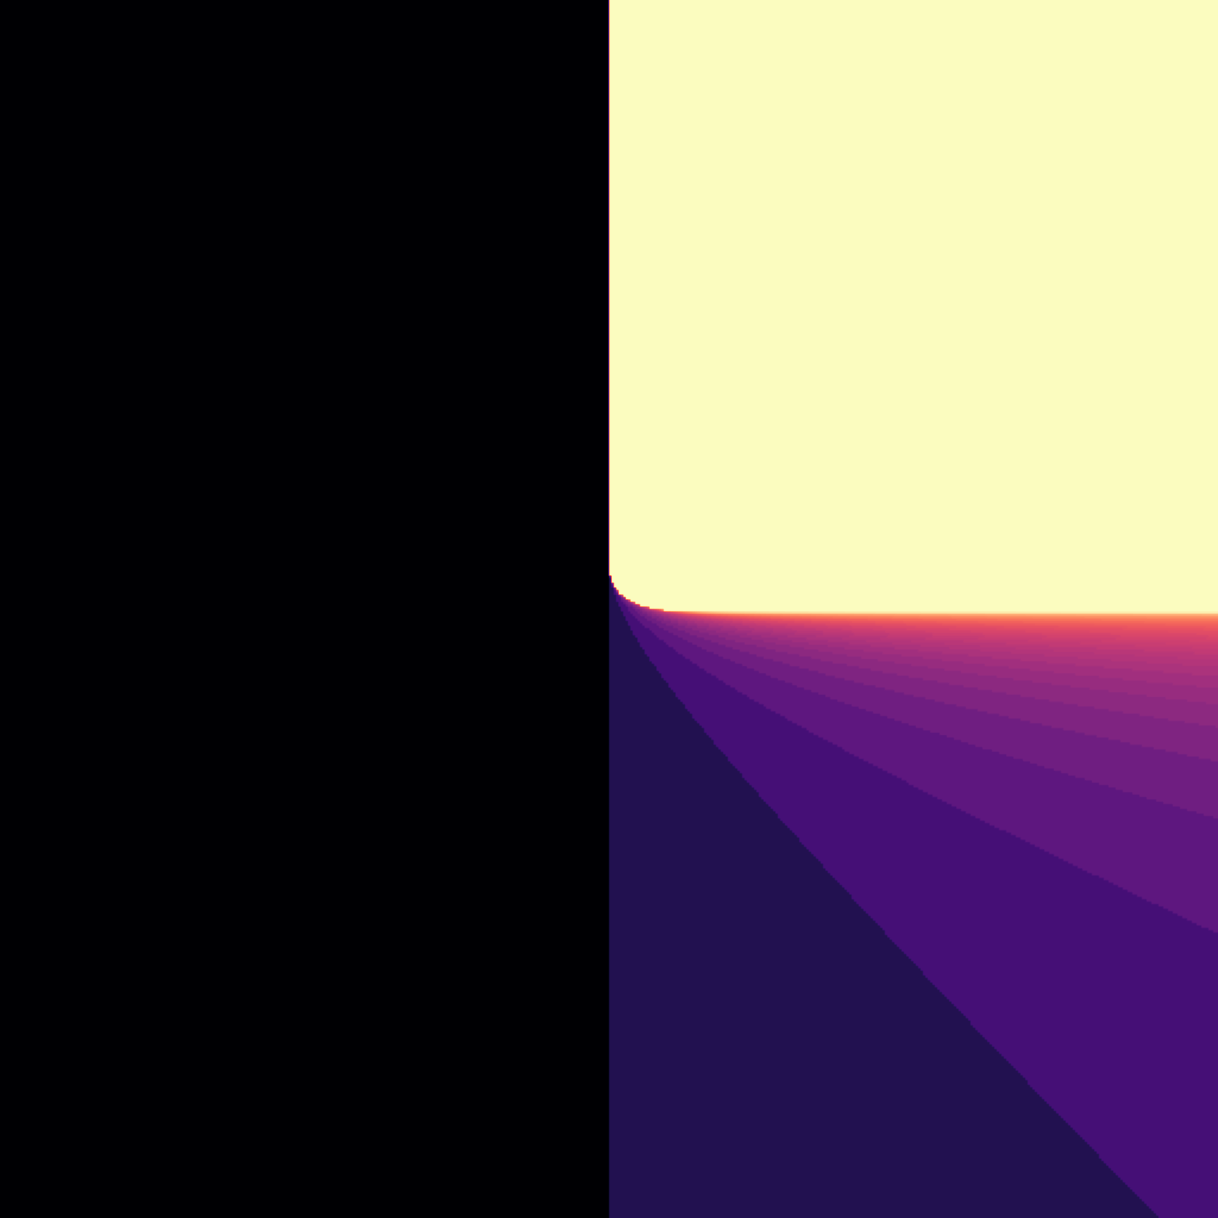
\includegraphics[interpolate=true,width=4.060000in,height=4.060000in]{single-neuron-impulse-response-img0.png}}%
\end{pgfscope}%
\begin{pgfscope}%
\pgfsetbuttcap%
\pgfsetroundjoin%
\definecolor{currentfill}{rgb}{0.000000,0.000000,0.000000}%
\pgfsetfillcolor{currentfill}%
\pgfsetlinewidth{0.803000pt}%
\definecolor{currentstroke}{rgb}{0.000000,0.000000,0.000000}%
\pgfsetstrokecolor{currentstroke}%
\pgfsetdash{}{0pt}%
\pgfsys@defobject{currentmarker}{\pgfqpoint{0.000000in}{-0.048611in}}{\pgfqpoint{0.000000in}{0.000000in}}{%
\pgfpathmoveto{\pgfqpoint{0.000000in}{0.000000in}}%
\pgfpathlineto{\pgfqpoint{0.000000in}{-0.048611in}}%
\pgfusepath{stroke,fill}%
}%
\begin{pgfscope}%
\pgfsys@transformshift{0.982003in}{0.920945in}%
\pgfsys@useobject{currentmarker}{}%
\end{pgfscope}%
\end{pgfscope}%
\begin{pgfscope}%
\definecolor{textcolor}{rgb}{0.000000,0.000000,0.000000}%
\pgfsetstrokecolor{textcolor}%
\pgfsetfillcolor{textcolor}%
\pgftext[x=0.982003in,y=0.823723in,,top]{\color{textcolor}{\rmfamily\fontsize{8.000000}{9.600000}\selectfont\catcode`\^=\active\def^{\ifmmode\sp\else\^{}\fi}\catcode`\%=\active\def%{\%}$\mathdefault{0}$}}%
\end{pgfscope}%
\begin{pgfscope}%
\pgfsetbuttcap%
\pgfsetroundjoin%
\definecolor{currentfill}{rgb}{0.000000,0.000000,0.000000}%
\pgfsetfillcolor{currentfill}%
\pgfsetlinewidth{0.803000pt}%
\definecolor{currentstroke}{rgb}{0.000000,0.000000,0.000000}%
\pgfsetstrokecolor{currentstroke}%
\pgfsetdash{}{0pt}%
\pgfsys@defobject{currentmarker}{\pgfqpoint{0.000000in}{-0.048611in}}{\pgfqpoint{0.000000in}{0.000000in}}{%
\pgfpathmoveto{\pgfqpoint{0.000000in}{0.000000in}}%
\pgfpathlineto{\pgfqpoint{0.000000in}{-0.048611in}}%
\pgfusepath{stroke,fill}%
}%
\begin{pgfscope}%
\pgfsys@transformshift{1.793889in}{0.920945in}%
\pgfsys@useobject{currentmarker}{}%
\end{pgfscope}%
\end{pgfscope}%
\begin{pgfscope}%
\definecolor{textcolor}{rgb}{0.000000,0.000000,0.000000}%
\pgfsetstrokecolor{textcolor}%
\pgfsetfillcolor{textcolor}%
\pgftext[x=1.793889in,y=0.823723in,,top]{\color{textcolor}{\rmfamily\fontsize{8.000000}{9.600000}\selectfont\catcode`\^=\active\def^{\ifmmode\sp\else\^{}\fi}\catcode`\%=\active\def%{\%}$\mathdefault{2}$}}%
\end{pgfscope}%
\begin{pgfscope}%
\pgfsetbuttcap%
\pgfsetroundjoin%
\definecolor{currentfill}{rgb}{0.000000,0.000000,0.000000}%
\pgfsetfillcolor{currentfill}%
\pgfsetlinewidth{0.803000pt}%
\definecolor{currentstroke}{rgb}{0.000000,0.000000,0.000000}%
\pgfsetstrokecolor{currentstroke}%
\pgfsetdash{}{0pt}%
\pgfsys@defobject{currentmarker}{\pgfqpoint{0.000000in}{-0.048611in}}{\pgfqpoint{0.000000in}{0.000000in}}{%
\pgfpathmoveto{\pgfqpoint{0.000000in}{0.000000in}}%
\pgfpathlineto{\pgfqpoint{0.000000in}{-0.048611in}}%
\pgfusepath{stroke,fill}%
}%
\begin{pgfscope}%
\pgfsys@transformshift{2.605775in}{0.920945in}%
\pgfsys@useobject{currentmarker}{}%
\end{pgfscope}%
\end{pgfscope}%
\begin{pgfscope}%
\definecolor{textcolor}{rgb}{0.000000,0.000000,0.000000}%
\pgfsetstrokecolor{textcolor}%
\pgfsetfillcolor{textcolor}%
\pgftext[x=2.605775in,y=0.823723in,,top]{\color{textcolor}{\rmfamily\fontsize{8.000000}{9.600000}\selectfont\catcode`\^=\active\def^{\ifmmode\sp\else\^{}\fi}\catcode`\%=\active\def%{\%}$\mathdefault{4}$}}%
\end{pgfscope}%
\begin{pgfscope}%
\pgfsetbuttcap%
\pgfsetroundjoin%
\definecolor{currentfill}{rgb}{0.000000,0.000000,0.000000}%
\pgfsetfillcolor{currentfill}%
\pgfsetlinewidth{0.803000pt}%
\definecolor{currentstroke}{rgb}{0.000000,0.000000,0.000000}%
\pgfsetstrokecolor{currentstroke}%
\pgfsetdash{}{0pt}%
\pgfsys@defobject{currentmarker}{\pgfqpoint{0.000000in}{-0.048611in}}{\pgfqpoint{0.000000in}{0.000000in}}{%
\pgfpathmoveto{\pgfqpoint{0.000000in}{0.000000in}}%
\pgfpathlineto{\pgfqpoint{0.000000in}{-0.048611in}}%
\pgfusepath{stroke,fill}%
}%
\begin{pgfscope}%
\pgfsys@transformshift{3.417660in}{0.920945in}%
\pgfsys@useobject{currentmarker}{}%
\end{pgfscope}%
\end{pgfscope}%
\begin{pgfscope}%
\definecolor{textcolor}{rgb}{0.000000,0.000000,0.000000}%
\pgfsetstrokecolor{textcolor}%
\pgfsetfillcolor{textcolor}%
\pgftext[x=3.417660in,y=0.823723in,,top]{\color{textcolor}{\rmfamily\fontsize{8.000000}{9.600000}\selectfont\catcode`\^=\active\def^{\ifmmode\sp\else\^{}\fi}\catcode`\%=\active\def%{\%}$\mathdefault{6}$}}%
\end{pgfscope}%
\begin{pgfscope}%
\pgfsetbuttcap%
\pgfsetroundjoin%
\definecolor{currentfill}{rgb}{0.000000,0.000000,0.000000}%
\pgfsetfillcolor{currentfill}%
\pgfsetlinewidth{0.803000pt}%
\definecolor{currentstroke}{rgb}{0.000000,0.000000,0.000000}%
\pgfsetstrokecolor{currentstroke}%
\pgfsetdash{}{0pt}%
\pgfsys@defobject{currentmarker}{\pgfqpoint{0.000000in}{-0.048611in}}{\pgfqpoint{0.000000in}{0.000000in}}{%
\pgfpathmoveto{\pgfqpoint{0.000000in}{0.000000in}}%
\pgfpathlineto{\pgfqpoint{0.000000in}{-0.048611in}}%
\pgfusepath{stroke,fill}%
}%
\begin{pgfscope}%
\pgfsys@transformshift{4.229546in}{0.920945in}%
\pgfsys@useobject{currentmarker}{}%
\end{pgfscope}%
\end{pgfscope}%
\begin{pgfscope}%
\definecolor{textcolor}{rgb}{0.000000,0.000000,0.000000}%
\pgfsetstrokecolor{textcolor}%
\pgfsetfillcolor{textcolor}%
\pgftext[x=4.229546in,y=0.823723in,,top]{\color{textcolor}{\rmfamily\fontsize{8.000000}{9.600000}\selectfont\catcode`\^=\active\def^{\ifmmode\sp\else\^{}\fi}\catcode`\%=\active\def%{\%}$\mathdefault{8}$}}%
\end{pgfscope}%
\begin{pgfscope}%
\definecolor{textcolor}{rgb}{0.000000,0.000000,0.000000}%
\pgfsetstrokecolor{textcolor}%
\pgfsetfillcolor{textcolor}%
\pgftext[x=2.605775in,y=0.660637in,,top]{\color{textcolor}{\rmfamily\fontsize{10.000000}{12.000000}\selectfont\catcode`\^=\active\def^{\ifmmode\sp\else\^{}\fi}\catcode`\%=\active\def%{\%}$w^f$}}%
\end{pgfscope}%
\begin{pgfscope}%
\pgfsetbuttcap%
\pgfsetroundjoin%
\definecolor{currentfill}{rgb}{0.000000,0.000000,0.000000}%
\pgfsetfillcolor{currentfill}%
\pgfsetlinewidth{0.803000pt}%
\definecolor{currentstroke}{rgb}{0.000000,0.000000,0.000000}%
\pgfsetstrokecolor{currentstroke}%
\pgfsetdash{}{0pt}%
\pgfsys@defobject{currentmarker}{\pgfqpoint{-0.048611in}{0.000000in}}{\pgfqpoint{-0.000000in}{0.000000in}}{%
\pgfpathmoveto{\pgfqpoint{-0.000000in}{0.000000in}}%
\pgfpathlineto{\pgfqpoint{-0.048611in}{0.000000in}}%
\pgfusepath{stroke,fill}%
}%
\begin{pgfscope}%
\pgfsys@transformshift{0.576061in}{1.245700in}%
\pgfsys@useobject{currentmarker}{}%
\end{pgfscope}%
\end{pgfscope}%
\begin{pgfscope}%
\definecolor{textcolor}{rgb}{0.000000,0.000000,0.000000}%
\pgfsetstrokecolor{textcolor}%
\pgfsetfillcolor{textcolor}%
\pgftext[x=0.327987in, y=1.203490in, left, base]{\color{textcolor}{\rmfamily\fontsize{8.000000}{9.600000}\selectfont\catcode`\^=\active\def^{\ifmmode\sp\else\^{}\fi}\catcode`\%=\active\def%{\%}$\mathdefault{\ensuremath{-}2}$}}%
\end{pgfscope}%
\begin{pgfscope}%
\pgfsetbuttcap%
\pgfsetroundjoin%
\definecolor{currentfill}{rgb}{0.000000,0.000000,0.000000}%
\pgfsetfillcolor{currentfill}%
\pgfsetlinewidth{0.803000pt}%
\definecolor{currentstroke}{rgb}{0.000000,0.000000,0.000000}%
\pgfsetstrokecolor{currentstroke}%
\pgfsetdash{}{0pt}%
\pgfsys@defobject{currentmarker}{\pgfqpoint{-0.048611in}{0.000000in}}{\pgfqpoint{-0.000000in}{0.000000in}}{%
\pgfpathmoveto{\pgfqpoint{-0.000000in}{0.000000in}}%
\pgfpathlineto{\pgfqpoint{-0.048611in}{0.000000in}}%
\pgfusepath{stroke,fill}%
}%
\begin{pgfscope}%
\pgfsys@transformshift{0.576061in}{2.057585in}%
\pgfsys@useobject{currentmarker}{}%
\end{pgfscope}%
\end{pgfscope}%
\begin{pgfscope}%
\definecolor{textcolor}{rgb}{0.000000,0.000000,0.000000}%
\pgfsetstrokecolor{textcolor}%
\pgfsetfillcolor{textcolor}%
\pgftext[x=0.419810in, y=2.015376in, left, base]{\color{textcolor}{\rmfamily\fontsize{8.000000}{9.600000}\selectfont\catcode`\^=\active\def^{\ifmmode\sp\else\^{}\fi}\catcode`\%=\active\def%{\%}$\mathdefault{0}$}}%
\end{pgfscope}%
\begin{pgfscope}%
\pgfsetbuttcap%
\pgfsetroundjoin%
\definecolor{currentfill}{rgb}{0.000000,0.000000,0.000000}%
\pgfsetfillcolor{currentfill}%
\pgfsetlinewidth{0.803000pt}%
\definecolor{currentstroke}{rgb}{0.000000,0.000000,0.000000}%
\pgfsetstrokecolor{currentstroke}%
\pgfsetdash{}{0pt}%
\pgfsys@defobject{currentmarker}{\pgfqpoint{-0.048611in}{0.000000in}}{\pgfqpoint{-0.000000in}{0.000000in}}{%
\pgfpathmoveto{\pgfqpoint{-0.000000in}{0.000000in}}%
\pgfpathlineto{\pgfqpoint{-0.048611in}{0.000000in}}%
\pgfusepath{stroke,fill}%
}%
\begin{pgfscope}%
\pgfsys@transformshift{0.576061in}{2.869471in}%
\pgfsys@useobject{currentmarker}{}%
\end{pgfscope}%
\end{pgfscope}%
\begin{pgfscope}%
\definecolor{textcolor}{rgb}{0.000000,0.000000,0.000000}%
\pgfsetstrokecolor{textcolor}%
\pgfsetfillcolor{textcolor}%
\pgftext[x=0.419810in, y=2.827262in, left, base]{\color{textcolor}{\rmfamily\fontsize{8.000000}{9.600000}\selectfont\catcode`\^=\active\def^{\ifmmode\sp\else\^{}\fi}\catcode`\%=\active\def%{\%}$\mathdefault{2}$}}%
\end{pgfscope}%
\begin{pgfscope}%
\pgfsetbuttcap%
\pgfsetroundjoin%
\definecolor{currentfill}{rgb}{0.000000,0.000000,0.000000}%
\pgfsetfillcolor{currentfill}%
\pgfsetlinewidth{0.803000pt}%
\definecolor{currentstroke}{rgb}{0.000000,0.000000,0.000000}%
\pgfsetstrokecolor{currentstroke}%
\pgfsetdash{}{0pt}%
\pgfsys@defobject{currentmarker}{\pgfqpoint{-0.048611in}{0.000000in}}{\pgfqpoint{-0.000000in}{0.000000in}}{%
\pgfpathmoveto{\pgfqpoint{-0.000000in}{0.000000in}}%
\pgfpathlineto{\pgfqpoint{-0.048611in}{0.000000in}}%
\pgfusepath{stroke,fill}%
}%
\begin{pgfscope}%
\pgfsys@transformshift{0.576061in}{3.681357in}%
\pgfsys@useobject{currentmarker}{}%
\end{pgfscope}%
\end{pgfscope}%
\begin{pgfscope}%
\definecolor{textcolor}{rgb}{0.000000,0.000000,0.000000}%
\pgfsetstrokecolor{textcolor}%
\pgfsetfillcolor{textcolor}%
\pgftext[x=0.419810in, y=3.639147in, left, base]{\color{textcolor}{\rmfamily\fontsize{8.000000}{9.600000}\selectfont\catcode`\^=\active\def^{\ifmmode\sp\else\^{}\fi}\catcode`\%=\active\def%{\%}$\mathdefault{4}$}}%
\end{pgfscope}%
\begin{pgfscope}%
\pgfsetbuttcap%
\pgfsetroundjoin%
\definecolor{currentfill}{rgb}{0.000000,0.000000,0.000000}%
\pgfsetfillcolor{currentfill}%
\pgfsetlinewidth{0.803000pt}%
\definecolor{currentstroke}{rgb}{0.000000,0.000000,0.000000}%
\pgfsetstrokecolor{currentstroke}%
\pgfsetdash{}{0pt}%
\pgfsys@defobject{currentmarker}{\pgfqpoint{-0.048611in}{0.000000in}}{\pgfqpoint{-0.000000in}{0.000000in}}{%
\pgfpathmoveto{\pgfqpoint{-0.000000in}{0.000000in}}%
\pgfpathlineto{\pgfqpoint{-0.048611in}{0.000000in}}%
\pgfusepath{stroke,fill}%
}%
\begin{pgfscope}%
\pgfsys@transformshift{0.576061in}{4.493242in}%
\pgfsys@useobject{currentmarker}{}%
\end{pgfscope}%
\end{pgfscope}%
\begin{pgfscope}%
\definecolor{textcolor}{rgb}{0.000000,0.000000,0.000000}%
\pgfsetstrokecolor{textcolor}%
\pgfsetfillcolor{textcolor}%
\pgftext[x=0.419810in, y=4.451033in, left, base]{\color{textcolor}{\rmfamily\fontsize{8.000000}{9.600000}\selectfont\catcode`\^=\active\def^{\ifmmode\sp\else\^{}\fi}\catcode`\%=\active\def%{\%}$\mathdefault{6}$}}%
\end{pgfscope}%
\begin{pgfscope}%
\definecolor{textcolor}{rgb}{0.000000,0.000000,0.000000}%
\pgfsetstrokecolor{textcolor}%
\pgfsetfillcolor{textcolor}%
\pgftext[x=0.272432in,y=2.950659in,,bottom,rotate=90.000000]{\color{textcolor}{\rmfamily\fontsize{10.000000}{12.000000}\selectfont\catcode`\^=\active\def^{\ifmmode\sp\else\^{}\fi}\catcode`\%=\active\def%{\%}$w^r$}}%
\end{pgfscope}%
\begin{pgfscope}%
\pgfsetrectcap%
\pgfsetmiterjoin%
\pgfsetlinewidth{0.803000pt}%
\definecolor{currentstroke}{rgb}{0.000000,0.000000,0.000000}%
\pgfsetstrokecolor{currentstroke}%
\pgfsetdash{}{0pt}%
\pgfpathmoveto{\pgfqpoint{0.576061in}{0.920945in}}%
\pgfpathlineto{\pgfqpoint{0.576061in}{4.980374in}}%
\pgfusepath{stroke}%
\end{pgfscope}%
\begin{pgfscope}%
\pgfsetrectcap%
\pgfsetmiterjoin%
\pgfsetlinewidth{0.803000pt}%
\definecolor{currentstroke}{rgb}{0.000000,0.000000,0.000000}%
\pgfsetstrokecolor{currentstroke}%
\pgfsetdash{}{0pt}%
\pgfpathmoveto{\pgfqpoint{4.635489in}{0.920945in}}%
\pgfpathlineto{\pgfqpoint{4.635489in}{4.980374in}}%
\pgfusepath{stroke}%
\end{pgfscope}%
\begin{pgfscope}%
\pgfsetrectcap%
\pgfsetmiterjoin%
\pgfsetlinewidth{0.803000pt}%
\definecolor{currentstroke}{rgb}{0.000000,0.000000,0.000000}%
\pgfsetstrokecolor{currentstroke}%
\pgfsetdash{}{0pt}%
\pgfpathmoveto{\pgfqpoint{0.576061in}{0.920945in}}%
\pgfpathlineto{\pgfqpoint{4.635489in}{0.920945in}}%
\pgfusepath{stroke}%
\end{pgfscope}%
\begin{pgfscope}%
\pgfsetrectcap%
\pgfsetmiterjoin%
\pgfsetlinewidth{0.803000pt}%
\definecolor{currentstroke}{rgb}{0.000000,0.000000,0.000000}%
\pgfsetstrokecolor{currentstroke}%
\pgfsetdash{}{0pt}%
\pgfpathmoveto{\pgfqpoint{0.576061in}{4.980374in}}%
\pgfpathlineto{\pgfqpoint{4.635489in}{4.980374in}}%
\pgfusepath{stroke}%
\end{pgfscope}%
\begin{pgfscope}%
\pgfsetbuttcap%
\pgfsetmiterjoin%
\definecolor{currentfill}{rgb}{1.000000,1.000000,1.000000}%
\pgfsetfillcolor{currentfill}%
\pgfsetlinewidth{0.000000pt}%
\definecolor{currentstroke}{rgb}{0.000000,0.000000,0.000000}%
\pgfsetstrokecolor{currentstroke}%
\pgfsetstrokeopacity{0.000000}%
\pgfsetdash{}{0pt}%
\pgfpathmoveto{\pgfqpoint{4.685489in}{0.920945in}}%
\pgfpathlineto{\pgfqpoint{4.888460in}{0.920945in}}%
\pgfpathlineto{\pgfqpoint{4.888460in}{4.980374in}}%
\pgfpathlineto{\pgfqpoint{4.685489in}{4.980374in}}%
\pgfpathlineto{\pgfqpoint{4.685489in}{0.920945in}}%
\pgfpathclose%
\pgfusepath{fill}%
\end{pgfscope}%
\begin{pgfscope}%
\pgfsys@transformshift{4.686667in}{0.920945in}%
\pgftext[left,bottom]{
\includegraphics[interpolate=true,width=0.203333in,height=4.060000in]{single-neuron-impulse-response-img1.png}}%
\end{pgfscope}%
\begin{pgfscope}%
\pgfsetbuttcap%
\pgfsetroundjoin%
\definecolor{currentfill}{rgb}{0.000000,0.000000,0.000000}%
\pgfsetfillcolor{currentfill}%
\pgfsetlinewidth{0.803000pt}%
\definecolor{currentstroke}{rgb}{0.000000,0.000000,0.000000}%
\pgfsetstrokecolor{currentstroke}%
\pgfsetdash{}{0pt}%
\pgfsys@defobject{currentmarker}{\pgfqpoint{0.000000in}{0.000000in}}{\pgfqpoint{0.048611in}{0.000000in}}{%
\pgfpathmoveto{\pgfqpoint{0.000000in}{0.000000in}}%
\pgfpathlineto{\pgfqpoint{0.048611in}{0.000000in}}%
\pgfusepath{stroke,fill}%
}%
\begin{pgfscope}%
\pgfsys@transformshift{4.888460in}{0.920945in}%
\pgfsys@useobject{currentmarker}{}%
\end{pgfscope}%
\end{pgfscope}%
\begin{pgfscope}%
\definecolor{textcolor}{rgb}{0.000000,0.000000,0.000000}%
\pgfsetstrokecolor{textcolor}%
\pgfsetfillcolor{textcolor}%
\pgftext[x=4.985683in, y=0.878736in, left, base]{\color{textcolor}{\rmfamily\fontsize{8.000000}{9.600000}\selectfont\catcode`\^=\active\def^{\ifmmode\sp\else\^{}\fi}\catcode`\%=\active\def%{\%}0.00}}%
\end{pgfscope}%
\begin{pgfscope}%
\pgfsetbuttcap%
\pgfsetroundjoin%
\definecolor{currentfill}{rgb}{0.000000,0.000000,0.000000}%
\pgfsetfillcolor{currentfill}%
\pgfsetlinewidth{0.803000pt}%
\definecolor{currentstroke}{rgb}{0.000000,0.000000,0.000000}%
\pgfsetstrokecolor{currentstroke}%
\pgfsetdash{}{0pt}%
\pgfsys@defobject{currentmarker}{\pgfqpoint{0.000000in}{0.000000in}}{\pgfqpoint{0.048611in}{0.000000in}}{%
\pgfpathmoveto{\pgfqpoint{0.000000in}{0.000000in}}%
\pgfpathlineto{\pgfqpoint{0.048611in}{0.000000in}}%
\pgfusepath{stroke,fill}%
}%
\begin{pgfscope}%
\pgfsys@transformshift{4.888460in}{1.371993in}%
\pgfsys@useobject{currentmarker}{}%
\end{pgfscope}%
\end{pgfscope}%
\begin{pgfscope}%
\definecolor{textcolor}{rgb}{0.000000,0.000000,0.000000}%
\pgfsetstrokecolor{textcolor}%
\pgfsetfillcolor{textcolor}%
\pgftext[x=4.985683in, y=1.329784in, left, base]{\color{textcolor}{\rmfamily\fontsize{8.000000}{9.600000}\selectfont\catcode`\^=\active\def^{\ifmmode\sp\else\^{}\fi}\catcode`\%=\active\def%{\%}0.72}}%
\end{pgfscope}%
\begin{pgfscope}%
\pgfsetbuttcap%
\pgfsetroundjoin%
\definecolor{currentfill}{rgb}{0.000000,0.000000,0.000000}%
\pgfsetfillcolor{currentfill}%
\pgfsetlinewidth{0.803000pt}%
\definecolor{currentstroke}{rgb}{0.000000,0.000000,0.000000}%
\pgfsetstrokecolor{currentstroke}%
\pgfsetdash{}{0pt}%
\pgfsys@defobject{currentmarker}{\pgfqpoint{0.000000in}{0.000000in}}{\pgfqpoint{0.048611in}{0.000000in}}{%
\pgfpathmoveto{\pgfqpoint{0.000000in}{0.000000in}}%
\pgfpathlineto{\pgfqpoint{0.048611in}{0.000000in}}%
\pgfusepath{stroke,fill}%
}%
\begin{pgfscope}%
\pgfsys@transformshift{4.888460in}{1.823041in}%
\pgfsys@useobject{currentmarker}{}%
\end{pgfscope}%
\end{pgfscope}%
\begin{pgfscope}%
\definecolor{textcolor}{rgb}{0.000000,0.000000,0.000000}%
\pgfsetstrokecolor{textcolor}%
\pgfsetfillcolor{textcolor}%
\pgftext[x=4.985683in, y=1.780831in, left, base]{\color{textcolor}{\rmfamily\fontsize{8.000000}{9.600000}\selectfont\catcode`\^=\active\def^{\ifmmode\sp\else\^{}\fi}\catcode`\%=\active\def%{\%}1.94}}%
\end{pgfscope}%
\begin{pgfscope}%
\pgfsetbuttcap%
\pgfsetroundjoin%
\definecolor{currentfill}{rgb}{0.000000,0.000000,0.000000}%
\pgfsetfillcolor{currentfill}%
\pgfsetlinewidth{0.803000pt}%
\definecolor{currentstroke}{rgb}{0.000000,0.000000,0.000000}%
\pgfsetstrokecolor{currentstroke}%
\pgfsetdash{}{0pt}%
\pgfsys@defobject{currentmarker}{\pgfqpoint{0.000000in}{0.000000in}}{\pgfqpoint{0.048611in}{0.000000in}}{%
\pgfpathmoveto{\pgfqpoint{0.000000in}{0.000000in}}%
\pgfpathlineto{\pgfqpoint{0.048611in}{0.000000in}}%
\pgfusepath{stroke,fill}%
}%
\begin{pgfscope}%
\pgfsys@transformshift{4.888460in}{2.274088in}%
\pgfsys@useobject{currentmarker}{}%
\end{pgfscope}%
\end{pgfscope}%
\begin{pgfscope}%
\definecolor{textcolor}{rgb}{0.000000,0.000000,0.000000}%
\pgfsetstrokecolor{textcolor}%
\pgfsetfillcolor{textcolor}%
\pgftext[x=4.985683in, y=2.231879in, left, base]{\color{textcolor}{\rmfamily\fontsize{8.000000}{9.600000}\selectfont\catcode`\^=\active\def^{\ifmmode\sp\else\^{}\fi}\catcode`\%=\active\def%{\%}4.05}}%
\end{pgfscope}%
\begin{pgfscope}%
\pgfsetbuttcap%
\pgfsetroundjoin%
\definecolor{currentfill}{rgb}{0.000000,0.000000,0.000000}%
\pgfsetfillcolor{currentfill}%
\pgfsetlinewidth{0.803000pt}%
\definecolor{currentstroke}{rgb}{0.000000,0.000000,0.000000}%
\pgfsetstrokecolor{currentstroke}%
\pgfsetdash{}{0pt}%
\pgfsys@defobject{currentmarker}{\pgfqpoint{0.000000in}{0.000000in}}{\pgfqpoint{0.048611in}{0.000000in}}{%
\pgfpathmoveto{\pgfqpoint{0.000000in}{0.000000in}}%
\pgfpathlineto{\pgfqpoint{0.048611in}{0.000000in}}%
\pgfusepath{stroke,fill}%
}%
\begin{pgfscope}%
\pgfsys@transformshift{4.888460in}{2.725136in}%
\pgfsys@useobject{currentmarker}{}%
\end{pgfscope}%
\end{pgfscope}%
\begin{pgfscope}%
\definecolor{textcolor}{rgb}{0.000000,0.000000,0.000000}%
\pgfsetstrokecolor{textcolor}%
\pgfsetfillcolor{textcolor}%
\pgftext[x=4.985683in, y=2.682926in, left, base]{\color{textcolor}{\rmfamily\fontsize{8.000000}{9.600000}\selectfont\catcode`\^=\active\def^{\ifmmode\sp\else\^{}\fi}\catcode`\%=\active\def%{\%}7.67}}%
\end{pgfscope}%
\begin{pgfscope}%
\pgfsetbuttcap%
\pgfsetroundjoin%
\definecolor{currentfill}{rgb}{0.000000,0.000000,0.000000}%
\pgfsetfillcolor{currentfill}%
\pgfsetlinewidth{0.803000pt}%
\definecolor{currentstroke}{rgb}{0.000000,0.000000,0.000000}%
\pgfsetstrokecolor{currentstroke}%
\pgfsetdash{}{0pt}%
\pgfsys@defobject{currentmarker}{\pgfqpoint{0.000000in}{0.000000in}}{\pgfqpoint{0.048611in}{0.000000in}}{%
\pgfpathmoveto{\pgfqpoint{0.000000in}{0.000000in}}%
\pgfpathlineto{\pgfqpoint{0.048611in}{0.000000in}}%
\pgfusepath{stroke,fill}%
}%
\begin{pgfscope}%
\pgfsys@transformshift{4.888460in}{3.176183in}%
\pgfsys@useobject{currentmarker}{}%
\end{pgfscope}%
\end{pgfscope}%
\begin{pgfscope}%
\definecolor{textcolor}{rgb}{0.000000,0.000000,0.000000}%
\pgfsetstrokecolor{textcolor}%
\pgfsetfillcolor{textcolor}%
\pgftext[x=4.985683in, y=3.133974in, left, base]{\color{textcolor}{\rmfamily\fontsize{8.000000}{9.600000}\selectfont\catcode`\^=\active\def^{\ifmmode\sp\else\^{}\fi}\catcode`\%=\active\def%{\%}13.88}}%
\end{pgfscope}%
\begin{pgfscope}%
\pgfsetbuttcap%
\pgfsetroundjoin%
\definecolor{currentfill}{rgb}{0.000000,0.000000,0.000000}%
\pgfsetfillcolor{currentfill}%
\pgfsetlinewidth{0.803000pt}%
\definecolor{currentstroke}{rgb}{0.000000,0.000000,0.000000}%
\pgfsetstrokecolor{currentstroke}%
\pgfsetdash{}{0pt}%
\pgfsys@defobject{currentmarker}{\pgfqpoint{0.000000in}{0.000000in}}{\pgfqpoint{0.048611in}{0.000000in}}{%
\pgfpathmoveto{\pgfqpoint{0.000000in}{0.000000in}}%
\pgfpathlineto{\pgfqpoint{0.048611in}{0.000000in}}%
\pgfusepath{stroke,fill}%
}%
\begin{pgfscope}%
\pgfsys@transformshift{4.888460in}{3.627231in}%
\pgfsys@useobject{currentmarker}{}%
\end{pgfscope}%
\end{pgfscope}%
\begin{pgfscope}%
\definecolor{textcolor}{rgb}{0.000000,0.000000,0.000000}%
\pgfsetstrokecolor{textcolor}%
\pgfsetfillcolor{textcolor}%
\pgftext[x=4.985683in, y=3.585022in, left, base]{\color{textcolor}{\rmfamily\fontsize{8.000000}{9.600000}\selectfont\catcode`\^=\active\def^{\ifmmode\sp\else\^{}\fi}\catcode`\%=\active\def%{\%}24.53}}%
\end{pgfscope}%
\begin{pgfscope}%
\pgfsetbuttcap%
\pgfsetroundjoin%
\definecolor{currentfill}{rgb}{0.000000,0.000000,0.000000}%
\pgfsetfillcolor{currentfill}%
\pgfsetlinewidth{0.803000pt}%
\definecolor{currentstroke}{rgb}{0.000000,0.000000,0.000000}%
\pgfsetstrokecolor{currentstroke}%
\pgfsetdash{}{0pt}%
\pgfsys@defobject{currentmarker}{\pgfqpoint{0.000000in}{0.000000in}}{\pgfqpoint{0.048611in}{0.000000in}}{%
\pgfpathmoveto{\pgfqpoint{0.000000in}{0.000000in}}%
\pgfpathlineto{\pgfqpoint{0.048611in}{0.000000in}}%
\pgfusepath{stroke,fill}%
}%
\begin{pgfscope}%
\pgfsys@transformshift{4.888460in}{4.078278in}%
\pgfsys@useobject{currentmarker}{}%
\end{pgfscope}%
\end{pgfscope}%
\begin{pgfscope}%
\definecolor{textcolor}{rgb}{0.000000,0.000000,0.000000}%
\pgfsetstrokecolor{textcolor}%
\pgfsetfillcolor{textcolor}%
\pgftext[x=4.985683in, y=4.036069in, left, base]{\color{textcolor}{\rmfamily\fontsize{8.000000}{9.600000}\selectfont\catcode`\^=\active\def^{\ifmmode\sp\else\^{}\fi}\catcode`\%=\active\def%{\%}42.81}}%
\end{pgfscope}%
\begin{pgfscope}%
\pgfsetbuttcap%
\pgfsetroundjoin%
\definecolor{currentfill}{rgb}{0.000000,0.000000,0.000000}%
\pgfsetfillcolor{currentfill}%
\pgfsetlinewidth{0.803000pt}%
\definecolor{currentstroke}{rgb}{0.000000,0.000000,0.000000}%
\pgfsetstrokecolor{currentstroke}%
\pgfsetdash{}{0pt}%
\pgfsys@defobject{currentmarker}{\pgfqpoint{0.000000in}{0.000000in}}{\pgfqpoint{0.048611in}{0.000000in}}{%
\pgfpathmoveto{\pgfqpoint{0.000000in}{0.000000in}}%
\pgfpathlineto{\pgfqpoint{0.048611in}{0.000000in}}%
\pgfusepath{stroke,fill}%
}%
\begin{pgfscope}%
\pgfsys@transformshift{4.888460in}{4.529326in}%
\pgfsys@useobject{currentmarker}{}%
\end{pgfscope}%
\end{pgfscope}%
\begin{pgfscope}%
\definecolor{textcolor}{rgb}{0.000000,0.000000,0.000000}%
\pgfsetstrokecolor{textcolor}%
\pgfsetfillcolor{textcolor}%
\pgftext[x=4.985683in, y=4.487117in, left, base]{\color{textcolor}{\rmfamily\fontsize{8.000000}{9.600000}\selectfont\catcode`\^=\active\def^{\ifmmode\sp\else\^{}\fi}\catcode`\%=\active\def%{\%}74.18}}%
\end{pgfscope}%
\begin{pgfscope}%
\pgfsetbuttcap%
\pgfsetroundjoin%
\definecolor{currentfill}{rgb}{0.000000,0.000000,0.000000}%
\pgfsetfillcolor{currentfill}%
\pgfsetlinewidth{0.803000pt}%
\definecolor{currentstroke}{rgb}{0.000000,0.000000,0.000000}%
\pgfsetstrokecolor{currentstroke}%
\pgfsetdash{}{0pt}%
\pgfsys@defobject{currentmarker}{\pgfqpoint{0.000000in}{0.000000in}}{\pgfqpoint{0.048611in}{0.000000in}}{%
\pgfpathmoveto{\pgfqpoint{0.000000in}{0.000000in}}%
\pgfpathlineto{\pgfqpoint{0.048611in}{0.000000in}}%
\pgfusepath{stroke,fill}%
}%
\begin{pgfscope}%
\pgfsys@transformshift{4.888460in}{4.980374in}%
\pgfsys@useobject{currentmarker}{}%
\end{pgfscope}%
\end{pgfscope}%
\begin{pgfscope}%
\definecolor{textcolor}{rgb}{0.000000,0.000000,0.000000}%
\pgfsetstrokecolor{textcolor}%
\pgfsetfillcolor{textcolor}%
\pgftext[x=4.985683in, y=4.938164in, left, base]{\color{textcolor}{\rmfamily\fontsize{8.000000}{9.600000}\selectfont\catcode`\^=\active\def^{\ifmmode\sp\else\^{}\fi}\catcode`\%=\active\def%{\%}128.00}}%
\end{pgfscope}%
\begin{pgfscope}%
\definecolor{textcolor}{rgb}{0.000000,0.000000,0.000000}%
\pgfsetstrokecolor{textcolor}%
\pgfsetfillcolor{textcolor}%
\pgftext[x=5.430018in,y=2.950659in,,top,rotate=90.000000]{\color{textcolor}{\rmfamily\fontsize{10.000000}{12.000000}\selectfont\catcode`\^=\active\def^{\ifmmode\sp\else\^{}\fi}\catcode`\%=\active\def%{\%}Number of emitted spikes}}%
\end{pgfscope}%
\begin{pgfscope}%
\pgfsetrectcap%
\pgfsetmiterjoin%
\pgfsetlinewidth{0.803000pt}%
\definecolor{currentstroke}{rgb}{0.000000,0.000000,0.000000}%
\pgfsetstrokecolor{currentstroke}%
\pgfsetdash{}{0pt}%
\pgfpathmoveto{\pgfqpoint{4.685489in}{0.920945in}}%
\pgfpathlineto{\pgfqpoint{4.786975in}{0.920945in}}%
\pgfpathlineto{\pgfqpoint{4.888460in}{0.920945in}}%
\pgfpathlineto{\pgfqpoint{4.888460in}{4.980374in}}%
\pgfpathlineto{\pgfqpoint{4.786975in}{4.980374in}}%
\pgfpathlineto{\pgfqpoint{4.685489in}{4.980374in}}%
\pgfpathlineto{\pgfqpoint{4.685489in}{0.920945in}}%
\pgfpathclose%
\pgfusepath{stroke}%
\end{pgfscope}%
\end{pgfpicture}%
\makeatother%
\endgroup%

  \caption{Number of emitted spikes of a LIF neuron in response to a single spike as a function of the feedforward weight $w^r$ and the recurrent weight $w^f$.}
  \label{impulse-response-figure}
\end{figure}

\subsection{Membrane dynamics in different regimes}
\begin{figure}[H]
  \centering
  %% Creator: Matplotlib, PGF backend
%%
%% To include the figure in your LaTeX document, write
%%   \input{<filename>.pgf}
%%
%% Make sure the required packages are loaded in your preamble
%%   \usepackage{pgf}
%%
%% Also ensure that all the required font packages are loaded; for instance,
%% the lmodern package is sometimes necessary when using math font.
%%   \usepackage{lmodern}
%%
%% Figures using additional raster images can only be included by \input if
%% they are in the same directory as the main LaTeX file. For loading figures
%% from other directories you can use the `import` package
%%   \usepackage{import}
%%
%% and then include the figures with
%%   \import{<path to file>}{<filename>.pgf}
%%
%% Matplotlib used the following preamble
%%   \def\mathdefault#1{#1}
%%   \everymath=\expandafter{\the\everymath\displaystyle}
%%   
%%   \usepackage{fontspec}
%%   \setmainfont{DejaVuSerif.ttf}[Path=\detokenize{/home/peter/recurrent-lif-layer-private/venv/lib/python3.10/site-packages/matplotlib/mpl-data/fonts/ttf/}]
%%   \setsansfont{DejaVuSans.ttf}[Path=\detokenize{/home/peter/recurrent-lif-layer-private/venv/lib/python3.10/site-packages/matplotlib/mpl-data/fonts/ttf/}]
%%   \setmonofont{DejaVuSansMono.ttf}[Path=\detokenize{/home/peter/recurrent-lif-layer-private/venv/lib/python3.10/site-packages/matplotlib/mpl-data/fonts/ttf/}]
%%   \makeatletter\@ifpackageloaded{underscore}{}{\usepackage[strings]{underscore}}\makeatother
%%
\begingroup%
\makeatletter%
\begin{pgfpicture}%
\pgfpathrectangle{\pgfpointorigin}{\pgfqpoint{6.267717in}{6.267717in}}%
\pgfusepath{use as bounding box, clip}%
\begin{pgfscope}%
\pgfsetbuttcap%
\pgfsetmiterjoin%
\definecolor{currentfill}{rgb}{1.000000,1.000000,1.000000}%
\pgfsetfillcolor{currentfill}%
\pgfsetlinewidth{0.000000pt}%
\definecolor{currentstroke}{rgb}{1.000000,1.000000,1.000000}%
\pgfsetstrokecolor{currentstroke}%
\pgfsetdash{}{0pt}%
\pgfpathmoveto{\pgfqpoint{0.000000in}{0.000000in}}%
\pgfpathlineto{\pgfqpoint{6.267717in}{0.000000in}}%
\pgfpathlineto{\pgfqpoint{6.267717in}{6.267717in}}%
\pgfpathlineto{\pgfqpoint{0.000000in}{6.267717in}}%
\pgfpathlineto{\pgfqpoint{0.000000in}{0.000000in}}%
\pgfpathclose%
\pgfusepath{fill}%
\end{pgfscope}%
\begin{pgfscope}%
\pgfsetbuttcap%
\pgfsetmiterjoin%
\definecolor{currentfill}{rgb}{1.000000,1.000000,1.000000}%
\pgfsetfillcolor{currentfill}%
\pgfsetlinewidth{0.000000pt}%
\definecolor{currentstroke}{rgb}{0.000000,0.000000,0.000000}%
\pgfsetstrokecolor{currentstroke}%
\pgfsetstrokeopacity{0.000000}%
\pgfsetdash{}{0pt}%
\pgfpathmoveto{\pgfqpoint{0.488989in}{4.326092in}}%
\pgfpathlineto{\pgfqpoint{6.117717in}{4.326092in}}%
\pgfpathlineto{\pgfqpoint{6.117717in}{5.909851in}}%
\pgfpathlineto{\pgfqpoint{0.488989in}{5.909851in}}%
\pgfpathlineto{\pgfqpoint{0.488989in}{4.326092in}}%
\pgfpathclose%
\pgfusepath{fill}%
\end{pgfscope}%
\begin{pgfscope}%
\pgfsetbuttcap%
\pgfsetroundjoin%
\definecolor{currentfill}{rgb}{0.000000,0.000000,0.000000}%
\pgfsetfillcolor{currentfill}%
\pgfsetlinewidth{0.803000pt}%
\definecolor{currentstroke}{rgb}{0.000000,0.000000,0.000000}%
\pgfsetstrokecolor{currentstroke}%
\pgfsetdash{}{0pt}%
\pgfsys@defobject{currentmarker}{\pgfqpoint{0.000000in}{-0.048611in}}{\pgfqpoint{0.000000in}{0.000000in}}{%
\pgfpathmoveto{\pgfqpoint{0.000000in}{0.000000in}}%
\pgfpathlineto{\pgfqpoint{0.000000in}{-0.048611in}}%
\pgfusepath{stroke,fill}%
}%
\begin{pgfscope}%
\pgfsys@transformshift{0.744060in}{4.326092in}%
\pgfsys@useobject{currentmarker}{}%
\end{pgfscope}%
\end{pgfscope}%
\begin{pgfscope}%
\pgfsetbuttcap%
\pgfsetroundjoin%
\definecolor{currentfill}{rgb}{0.000000,0.000000,0.000000}%
\pgfsetfillcolor{currentfill}%
\pgfsetlinewidth{0.803000pt}%
\definecolor{currentstroke}{rgb}{0.000000,0.000000,0.000000}%
\pgfsetstrokecolor{currentstroke}%
\pgfsetdash{}{0pt}%
\pgfsys@defobject{currentmarker}{\pgfqpoint{0.000000in}{-0.048611in}}{\pgfqpoint{0.000000in}{0.000000in}}{%
\pgfpathmoveto{\pgfqpoint{0.000000in}{0.000000in}}%
\pgfpathlineto{\pgfqpoint{0.000000in}{-0.048611in}}%
\pgfusepath{stroke,fill}%
}%
\begin{pgfscope}%
\pgfsys@transformshift{1.426176in}{4.326092in}%
\pgfsys@useobject{currentmarker}{}%
\end{pgfscope}%
\end{pgfscope}%
\begin{pgfscope}%
\pgfsetbuttcap%
\pgfsetroundjoin%
\definecolor{currentfill}{rgb}{0.000000,0.000000,0.000000}%
\pgfsetfillcolor{currentfill}%
\pgfsetlinewidth{0.803000pt}%
\definecolor{currentstroke}{rgb}{0.000000,0.000000,0.000000}%
\pgfsetstrokecolor{currentstroke}%
\pgfsetdash{}{0pt}%
\pgfsys@defobject{currentmarker}{\pgfqpoint{0.000000in}{-0.048611in}}{\pgfqpoint{0.000000in}{0.000000in}}{%
\pgfpathmoveto{\pgfqpoint{0.000000in}{0.000000in}}%
\pgfpathlineto{\pgfqpoint{0.000000in}{-0.048611in}}%
\pgfusepath{stroke,fill}%
}%
\begin{pgfscope}%
\pgfsys@transformshift{2.108292in}{4.326092in}%
\pgfsys@useobject{currentmarker}{}%
\end{pgfscope}%
\end{pgfscope}%
\begin{pgfscope}%
\pgfsetbuttcap%
\pgfsetroundjoin%
\definecolor{currentfill}{rgb}{0.000000,0.000000,0.000000}%
\pgfsetfillcolor{currentfill}%
\pgfsetlinewidth{0.803000pt}%
\definecolor{currentstroke}{rgb}{0.000000,0.000000,0.000000}%
\pgfsetstrokecolor{currentstroke}%
\pgfsetdash{}{0pt}%
\pgfsys@defobject{currentmarker}{\pgfqpoint{0.000000in}{-0.048611in}}{\pgfqpoint{0.000000in}{0.000000in}}{%
\pgfpathmoveto{\pgfqpoint{0.000000in}{0.000000in}}%
\pgfpathlineto{\pgfqpoint{0.000000in}{-0.048611in}}%
\pgfusepath{stroke,fill}%
}%
\begin{pgfscope}%
\pgfsys@transformshift{2.790408in}{4.326092in}%
\pgfsys@useobject{currentmarker}{}%
\end{pgfscope}%
\end{pgfscope}%
\begin{pgfscope}%
\pgfsetbuttcap%
\pgfsetroundjoin%
\definecolor{currentfill}{rgb}{0.000000,0.000000,0.000000}%
\pgfsetfillcolor{currentfill}%
\pgfsetlinewidth{0.803000pt}%
\definecolor{currentstroke}{rgb}{0.000000,0.000000,0.000000}%
\pgfsetstrokecolor{currentstroke}%
\pgfsetdash{}{0pt}%
\pgfsys@defobject{currentmarker}{\pgfqpoint{0.000000in}{-0.048611in}}{\pgfqpoint{0.000000in}{0.000000in}}{%
\pgfpathmoveto{\pgfqpoint{0.000000in}{0.000000in}}%
\pgfpathlineto{\pgfqpoint{0.000000in}{-0.048611in}}%
\pgfusepath{stroke,fill}%
}%
\begin{pgfscope}%
\pgfsys@transformshift{3.472524in}{4.326092in}%
\pgfsys@useobject{currentmarker}{}%
\end{pgfscope}%
\end{pgfscope}%
\begin{pgfscope}%
\pgfsetbuttcap%
\pgfsetroundjoin%
\definecolor{currentfill}{rgb}{0.000000,0.000000,0.000000}%
\pgfsetfillcolor{currentfill}%
\pgfsetlinewidth{0.803000pt}%
\definecolor{currentstroke}{rgb}{0.000000,0.000000,0.000000}%
\pgfsetstrokecolor{currentstroke}%
\pgfsetdash{}{0pt}%
\pgfsys@defobject{currentmarker}{\pgfqpoint{0.000000in}{-0.048611in}}{\pgfqpoint{0.000000in}{0.000000in}}{%
\pgfpathmoveto{\pgfqpoint{0.000000in}{0.000000in}}%
\pgfpathlineto{\pgfqpoint{0.000000in}{-0.048611in}}%
\pgfusepath{stroke,fill}%
}%
\begin{pgfscope}%
\pgfsys@transformshift{4.154640in}{4.326092in}%
\pgfsys@useobject{currentmarker}{}%
\end{pgfscope}%
\end{pgfscope}%
\begin{pgfscope}%
\pgfsetbuttcap%
\pgfsetroundjoin%
\definecolor{currentfill}{rgb}{0.000000,0.000000,0.000000}%
\pgfsetfillcolor{currentfill}%
\pgfsetlinewidth{0.803000pt}%
\definecolor{currentstroke}{rgb}{0.000000,0.000000,0.000000}%
\pgfsetstrokecolor{currentstroke}%
\pgfsetdash{}{0pt}%
\pgfsys@defobject{currentmarker}{\pgfqpoint{0.000000in}{-0.048611in}}{\pgfqpoint{0.000000in}{0.000000in}}{%
\pgfpathmoveto{\pgfqpoint{0.000000in}{0.000000in}}%
\pgfpathlineto{\pgfqpoint{0.000000in}{-0.048611in}}%
\pgfusepath{stroke,fill}%
}%
\begin{pgfscope}%
\pgfsys@transformshift{4.836756in}{4.326092in}%
\pgfsys@useobject{currentmarker}{}%
\end{pgfscope}%
\end{pgfscope}%
\begin{pgfscope}%
\pgfsetbuttcap%
\pgfsetroundjoin%
\definecolor{currentfill}{rgb}{0.000000,0.000000,0.000000}%
\pgfsetfillcolor{currentfill}%
\pgfsetlinewidth{0.803000pt}%
\definecolor{currentstroke}{rgb}{0.000000,0.000000,0.000000}%
\pgfsetstrokecolor{currentstroke}%
\pgfsetdash{}{0pt}%
\pgfsys@defobject{currentmarker}{\pgfqpoint{0.000000in}{-0.048611in}}{\pgfqpoint{0.000000in}{0.000000in}}{%
\pgfpathmoveto{\pgfqpoint{0.000000in}{0.000000in}}%
\pgfpathlineto{\pgfqpoint{0.000000in}{-0.048611in}}%
\pgfusepath{stroke,fill}%
}%
\begin{pgfscope}%
\pgfsys@transformshift{5.518872in}{4.326092in}%
\pgfsys@useobject{currentmarker}{}%
\end{pgfscope}%
\end{pgfscope}%
\begin{pgfscope}%
\pgfsetbuttcap%
\pgfsetroundjoin%
\definecolor{currentfill}{rgb}{0.000000,0.000000,0.000000}%
\pgfsetfillcolor{currentfill}%
\pgfsetlinewidth{0.803000pt}%
\definecolor{currentstroke}{rgb}{0.000000,0.000000,0.000000}%
\pgfsetstrokecolor{currentstroke}%
\pgfsetdash{}{0pt}%
\pgfsys@defobject{currentmarker}{\pgfqpoint{-0.048611in}{0.000000in}}{\pgfqpoint{-0.000000in}{0.000000in}}{%
\pgfpathmoveto{\pgfqpoint{-0.000000in}{0.000000in}}%
\pgfpathlineto{\pgfqpoint{-0.048611in}{0.000000in}}%
\pgfusepath{stroke,fill}%
}%
\begin{pgfscope}%
\pgfsys@transformshift{0.488989in}{4.398081in}%
\pgfsys@useobject{currentmarker}{}%
\end{pgfscope}%
\end{pgfscope}%
\begin{pgfscope}%
\definecolor{textcolor}{rgb}{0.000000,0.000000,0.000000}%
\pgfsetstrokecolor{textcolor}%
\pgfsetfillcolor{textcolor}%
\pgftext[x=0.240916in, y=4.355871in, left, base]{\color{textcolor}{\rmfamily\fontsize{8.000000}{9.600000}\selectfont\catcode`\^=\active\def^{\ifmmode\sp\else\^{}\fi}\catcode`\%=\active\def%{\%}$\mathdefault{0.0}$}}%
\end{pgfscope}%
\begin{pgfscope}%
\pgfsetbuttcap%
\pgfsetroundjoin%
\definecolor{currentfill}{rgb}{0.000000,0.000000,0.000000}%
\pgfsetfillcolor{currentfill}%
\pgfsetlinewidth{0.803000pt}%
\definecolor{currentstroke}{rgb}{0.000000,0.000000,0.000000}%
\pgfsetstrokecolor{currentstroke}%
\pgfsetdash{}{0pt}%
\pgfsys@defobject{currentmarker}{\pgfqpoint{-0.048611in}{0.000000in}}{\pgfqpoint{-0.000000in}{0.000000in}}{%
\pgfpathmoveto{\pgfqpoint{-0.000000in}{0.000000in}}%
\pgfpathlineto{\pgfqpoint{-0.048611in}{0.000000in}}%
\pgfusepath{stroke,fill}%
}%
\begin{pgfscope}%
\pgfsys@transformshift{0.488989in}{4.686037in}%
\pgfsys@useobject{currentmarker}{}%
\end{pgfscope}%
\end{pgfscope}%
\begin{pgfscope}%
\definecolor{textcolor}{rgb}{0.000000,0.000000,0.000000}%
\pgfsetstrokecolor{textcolor}%
\pgfsetfillcolor{textcolor}%
\pgftext[x=0.240916in, y=4.643828in, left, base]{\color{textcolor}{\rmfamily\fontsize{8.000000}{9.600000}\selectfont\catcode`\^=\active\def^{\ifmmode\sp\else\^{}\fi}\catcode`\%=\active\def%{\%}$\mathdefault{0.2}$}}%
\end{pgfscope}%
\begin{pgfscope}%
\pgfsetbuttcap%
\pgfsetroundjoin%
\definecolor{currentfill}{rgb}{0.000000,0.000000,0.000000}%
\pgfsetfillcolor{currentfill}%
\pgfsetlinewidth{0.803000pt}%
\definecolor{currentstroke}{rgb}{0.000000,0.000000,0.000000}%
\pgfsetstrokecolor{currentstroke}%
\pgfsetdash{}{0pt}%
\pgfsys@defobject{currentmarker}{\pgfqpoint{-0.048611in}{0.000000in}}{\pgfqpoint{-0.000000in}{0.000000in}}{%
\pgfpathmoveto{\pgfqpoint{-0.000000in}{0.000000in}}%
\pgfpathlineto{\pgfqpoint{-0.048611in}{0.000000in}}%
\pgfusepath{stroke,fill}%
}%
\begin{pgfscope}%
\pgfsys@transformshift{0.488989in}{4.973993in}%
\pgfsys@useobject{currentmarker}{}%
\end{pgfscope}%
\end{pgfscope}%
\begin{pgfscope}%
\definecolor{textcolor}{rgb}{0.000000,0.000000,0.000000}%
\pgfsetstrokecolor{textcolor}%
\pgfsetfillcolor{textcolor}%
\pgftext[x=0.240916in, y=4.931784in, left, base]{\color{textcolor}{\rmfamily\fontsize{8.000000}{9.600000}\selectfont\catcode`\^=\active\def^{\ifmmode\sp\else\^{}\fi}\catcode`\%=\active\def%{\%}$\mathdefault{0.4}$}}%
\end{pgfscope}%
\begin{pgfscope}%
\pgfsetbuttcap%
\pgfsetroundjoin%
\definecolor{currentfill}{rgb}{0.000000,0.000000,0.000000}%
\pgfsetfillcolor{currentfill}%
\pgfsetlinewidth{0.803000pt}%
\definecolor{currentstroke}{rgb}{0.000000,0.000000,0.000000}%
\pgfsetstrokecolor{currentstroke}%
\pgfsetdash{}{0pt}%
\pgfsys@defobject{currentmarker}{\pgfqpoint{-0.048611in}{0.000000in}}{\pgfqpoint{-0.000000in}{0.000000in}}{%
\pgfpathmoveto{\pgfqpoint{-0.000000in}{0.000000in}}%
\pgfpathlineto{\pgfqpoint{-0.048611in}{0.000000in}}%
\pgfusepath{stroke,fill}%
}%
\begin{pgfscope}%
\pgfsys@transformshift{0.488989in}{5.261949in}%
\pgfsys@useobject{currentmarker}{}%
\end{pgfscope}%
\end{pgfscope}%
\begin{pgfscope}%
\definecolor{textcolor}{rgb}{0.000000,0.000000,0.000000}%
\pgfsetstrokecolor{textcolor}%
\pgfsetfillcolor{textcolor}%
\pgftext[x=0.240916in, y=5.219740in, left, base]{\color{textcolor}{\rmfamily\fontsize{8.000000}{9.600000}\selectfont\catcode`\^=\active\def^{\ifmmode\sp\else\^{}\fi}\catcode`\%=\active\def%{\%}$\mathdefault{0.6}$}}%
\end{pgfscope}%
\begin{pgfscope}%
\pgfsetbuttcap%
\pgfsetroundjoin%
\definecolor{currentfill}{rgb}{0.000000,0.000000,0.000000}%
\pgfsetfillcolor{currentfill}%
\pgfsetlinewidth{0.803000pt}%
\definecolor{currentstroke}{rgb}{0.000000,0.000000,0.000000}%
\pgfsetstrokecolor{currentstroke}%
\pgfsetdash{}{0pt}%
\pgfsys@defobject{currentmarker}{\pgfqpoint{-0.048611in}{0.000000in}}{\pgfqpoint{-0.000000in}{0.000000in}}{%
\pgfpathmoveto{\pgfqpoint{-0.000000in}{0.000000in}}%
\pgfpathlineto{\pgfqpoint{-0.048611in}{0.000000in}}%
\pgfusepath{stroke,fill}%
}%
\begin{pgfscope}%
\pgfsys@transformshift{0.488989in}{5.549905in}%
\pgfsys@useobject{currentmarker}{}%
\end{pgfscope}%
\end{pgfscope}%
\begin{pgfscope}%
\definecolor{textcolor}{rgb}{0.000000,0.000000,0.000000}%
\pgfsetstrokecolor{textcolor}%
\pgfsetfillcolor{textcolor}%
\pgftext[x=0.240916in, y=5.507696in, left, base]{\color{textcolor}{\rmfamily\fontsize{8.000000}{9.600000}\selectfont\catcode`\^=\active\def^{\ifmmode\sp\else\^{}\fi}\catcode`\%=\active\def%{\%}$\mathdefault{0.8}$}}%
\end{pgfscope}%
\begin{pgfscope}%
\pgfsetbuttcap%
\pgfsetroundjoin%
\definecolor{currentfill}{rgb}{0.000000,0.000000,0.000000}%
\pgfsetfillcolor{currentfill}%
\pgfsetlinewidth{0.803000pt}%
\definecolor{currentstroke}{rgb}{0.000000,0.000000,0.000000}%
\pgfsetstrokecolor{currentstroke}%
\pgfsetdash{}{0pt}%
\pgfsys@defobject{currentmarker}{\pgfqpoint{-0.048611in}{0.000000in}}{\pgfqpoint{-0.000000in}{0.000000in}}{%
\pgfpathmoveto{\pgfqpoint{-0.000000in}{0.000000in}}%
\pgfpathlineto{\pgfqpoint{-0.048611in}{0.000000in}}%
\pgfusepath{stroke,fill}%
}%
\begin{pgfscope}%
\pgfsys@transformshift{0.488989in}{5.837862in}%
\pgfsys@useobject{currentmarker}{}%
\end{pgfscope}%
\end{pgfscope}%
\begin{pgfscope}%
\definecolor{textcolor}{rgb}{0.000000,0.000000,0.000000}%
\pgfsetstrokecolor{textcolor}%
\pgfsetfillcolor{textcolor}%
\pgftext[x=0.240916in, y=5.795652in, left, base]{\color{textcolor}{\rmfamily\fontsize{8.000000}{9.600000}\selectfont\catcode`\^=\active\def^{\ifmmode\sp\else\^{}\fi}\catcode`\%=\active\def%{\%}$\mathdefault{1.0}$}}%
\end{pgfscope}%
\begin{pgfscope}%
\pgfpathrectangle{\pgfqpoint{0.488989in}{4.326092in}}{\pgfqpoint{5.628728in}{1.583759in}}%
\pgfusepath{clip}%
\pgfsetrectcap%
\pgfsetroundjoin%
\pgfsetlinewidth{1.505625pt}%
\definecolor{currentstroke}{rgb}{0.121569,0.466667,0.705882}%
\pgfsetstrokecolor{currentstroke}%
\pgfsetstrokeopacity{0.800000}%
\pgfsetdash{}{0pt}%
\pgfpathmoveto{\pgfqpoint{0.744840in}{4.398081in}}%
\pgfpathlineto{\pgfqpoint{0.763939in}{4.468301in}}%
\pgfpathlineto{\pgfqpoint{0.783039in}{4.535607in}}%
\pgfpathlineto{\pgfqpoint{0.802138in}{4.600091in}}%
\pgfpathlineto{\pgfqpoint{0.821237in}{4.661845in}}%
\pgfpathlineto{\pgfqpoint{0.840336in}{4.720959in}}%
\pgfpathlineto{\pgfqpoint{0.859436in}{4.777517in}}%
\pgfpathlineto{\pgfqpoint{0.877171in}{4.827820in}}%
\pgfpathlineto{\pgfqpoint{0.894906in}{4.876056in}}%
\pgfpathlineto{\pgfqpoint{0.912641in}{4.922289in}}%
\pgfpathlineto{\pgfqpoint{0.930376in}{4.966580in}}%
\pgfpathlineto{\pgfqpoint{0.948111in}{5.008989in}}%
\pgfpathlineto{\pgfqpoint{0.965846in}{5.049572in}}%
\pgfpathlineto{\pgfqpoint{0.983581in}{5.088388in}}%
\pgfpathlineto{\pgfqpoint{1.001316in}{5.125490in}}%
\pgfpathlineto{\pgfqpoint{1.019051in}{5.160932in}}%
\pgfpathlineto{\pgfqpoint{1.036786in}{5.194765in}}%
\pgfpathlineto{\pgfqpoint{1.054521in}{5.227040in}}%
\pgfpathlineto{\pgfqpoint{1.072256in}{5.257806in}}%
\pgfpathlineto{\pgfqpoint{1.089991in}{5.287110in}}%
\pgfpathlineto{\pgfqpoint{1.107726in}{5.314999in}}%
\pgfpathlineto{\pgfqpoint{1.125461in}{5.341516in}}%
\pgfpathlineto{\pgfqpoint{1.143196in}{5.366707in}}%
\pgfpathlineto{\pgfqpoint{1.160931in}{5.390613in}}%
\pgfpathlineto{\pgfqpoint{1.178666in}{5.413276in}}%
\pgfpathlineto{\pgfqpoint{1.196401in}{5.434736in}}%
\pgfpathlineto{\pgfqpoint{1.214136in}{5.455031in}}%
\pgfpathlineto{\pgfqpoint{1.231871in}{5.474199in}}%
\pgfpathlineto{\pgfqpoint{1.249606in}{5.492278in}}%
\pgfpathlineto{\pgfqpoint{1.267341in}{5.509302in}}%
\pgfpathlineto{\pgfqpoint{1.285076in}{5.525307in}}%
\pgfpathlineto{\pgfqpoint{1.302811in}{5.540326in}}%
\pgfpathlineto{\pgfqpoint{1.320546in}{5.554391in}}%
\pgfpathlineto{\pgfqpoint{1.338281in}{5.567536in}}%
\pgfpathlineto{\pgfqpoint{1.356016in}{5.579790in}}%
\pgfpathlineto{\pgfqpoint{1.373751in}{5.591184in}}%
\pgfpathlineto{\pgfqpoint{1.376479in}{5.602226in}}%
\pgfpathlineto{\pgfqpoint{1.394215in}{5.677600in}}%
\pgfpathlineto{\pgfqpoint{1.411950in}{5.749666in}}%
\pgfpathlineto{\pgfqpoint{1.429685in}{5.818528in}}%
\pgfpathlineto{\pgfqpoint{1.435141in}{5.837862in}}%
\pgfpathlineto{\pgfqpoint{1.436506in}{5.117971in}}%
\pgfpathlineto{\pgfqpoint{3.679303in}{5.117971in}}%
\pgfpathlineto{\pgfqpoint{3.679303in}{5.117971in}}%
\pgfusepath{stroke}%
\end{pgfscope}%
\begin{pgfscope}%
\pgfpathrectangle{\pgfqpoint{0.488989in}{4.326092in}}{\pgfqpoint{5.628728in}{1.583759in}}%
\pgfusepath{clip}%
\pgfsetbuttcap%
\pgfsetroundjoin%
\pgfsetlinewidth{1.505625pt}%
\definecolor{currentstroke}{rgb}{0.501961,0.501961,0.501961}%
\pgfsetstrokecolor{currentstroke}%
\pgfsetstrokeopacity{0.200000}%
\pgfsetdash{{5.550000pt}{2.400000pt}}{0.000000pt}%
\pgfpathmoveto{\pgfqpoint{3.588634in}{4.326092in}}%
\pgfpathlineto{\pgfqpoint{3.588634in}{5.909851in}}%
\pgfusepath{stroke}%
\end{pgfscope}%
\begin{pgfscope}%
\pgfpathrectangle{\pgfqpoint{0.488989in}{4.326092in}}{\pgfqpoint{5.628728in}{1.583759in}}%
\pgfusepath{clip}%
\pgfsetbuttcap%
\pgfsetroundjoin%
\pgfsetlinewidth{1.505625pt}%
\definecolor{currentstroke}{rgb}{0.501961,0.501961,0.501961}%
\pgfsetstrokecolor{currentstroke}%
\pgfsetstrokeopacity{0.200000}%
\pgfsetdash{{5.550000pt}{2.400000pt}}{0.000000pt}%
\pgfpathmoveto{\pgfqpoint{5.657508in}{4.326092in}}%
\pgfpathlineto{\pgfqpoint{5.657508in}{5.909851in}}%
\pgfusepath{stroke}%
\end{pgfscope}%
\begin{pgfscope}%
\pgfpathrectangle{\pgfqpoint{0.488989in}{4.326092in}}{\pgfqpoint{5.628728in}{1.583759in}}%
\pgfusepath{clip}%
\pgfsetbuttcap%
\pgfsetroundjoin%
\pgfsetlinewidth{1.505625pt}%
\definecolor{currentstroke}{rgb}{0.501961,0.501961,0.501961}%
\pgfsetstrokecolor{currentstroke}%
\pgfsetstrokeopacity{0.200000}%
\pgfsetdash{{5.550000pt}{2.400000pt}}{0.000000pt}%
\pgfpathmoveto{\pgfqpoint{0.744840in}{4.326092in}}%
\pgfpathlineto{\pgfqpoint{0.744840in}{5.909851in}}%
\pgfusepath{stroke}%
\end{pgfscope}%
\begin{pgfscope}%
\pgfpathrectangle{\pgfqpoint{0.488989in}{4.326092in}}{\pgfqpoint{5.628728in}{1.583759in}}%
\pgfusepath{clip}%
\pgfsetbuttcap%
\pgfsetroundjoin%
\pgfsetlinewidth{1.505625pt}%
\definecolor{currentstroke}{rgb}{0.501961,0.501961,0.501961}%
\pgfsetstrokecolor{currentstroke}%
\pgfsetstrokeopacity{0.200000}%
\pgfsetdash{{5.550000pt}{2.400000pt}}{0.000000pt}%
\pgfpathmoveto{\pgfqpoint{2.806319in}{4.326092in}}%
\pgfpathlineto{\pgfqpoint{2.806319in}{5.909851in}}%
\pgfusepath{stroke}%
\end{pgfscope}%
\begin{pgfscope}%
\pgfpathrectangle{\pgfqpoint{0.488989in}{4.326092in}}{\pgfqpoint{5.628728in}{1.583759in}}%
\pgfusepath{clip}%
\pgfsetbuttcap%
\pgfsetroundjoin%
\pgfsetlinewidth{1.505625pt}%
\definecolor{currentstroke}{rgb}{0.501961,0.501961,0.501961}%
\pgfsetstrokecolor{currentstroke}%
\pgfsetstrokeopacity{0.200000}%
\pgfsetdash{{5.550000pt}{2.400000pt}}{0.000000pt}%
\pgfpathmoveto{\pgfqpoint{1.745105in}{4.326092in}}%
\pgfpathlineto{\pgfqpoint{1.745105in}{5.909851in}}%
\pgfusepath{stroke}%
\end{pgfscope}%
\begin{pgfscope}%
\pgfpathrectangle{\pgfqpoint{0.488989in}{4.326092in}}{\pgfqpoint{5.628728in}{1.583759in}}%
\pgfusepath{clip}%
\pgfsetbuttcap%
\pgfsetroundjoin%
\pgfsetlinewidth{1.505625pt}%
\definecolor{currentstroke}{rgb}{0.501961,0.501961,0.501961}%
\pgfsetstrokecolor{currentstroke}%
\pgfsetstrokeopacity{0.200000}%
\pgfsetdash{{5.550000pt}{2.400000pt}}{0.000000pt}%
\pgfpathmoveto{\pgfqpoint{1.373916in}{4.326092in}}%
\pgfpathlineto{\pgfqpoint{1.373916in}{5.909851in}}%
\pgfusepath{stroke}%
\end{pgfscope}%
\begin{pgfscope}%
\pgfpathrectangle{\pgfqpoint{0.488989in}{4.326092in}}{\pgfqpoint{5.628728in}{1.583759in}}%
\pgfusepath{clip}%
\pgfsetbuttcap%
\pgfsetroundjoin%
\pgfsetlinewidth{1.505625pt}%
\definecolor{currentstroke}{rgb}{0.501961,0.501961,0.501961}%
\pgfsetstrokecolor{currentstroke}%
\pgfsetstrokeopacity{0.200000}%
\pgfsetdash{{5.550000pt}{2.400000pt}}{0.000000pt}%
\pgfusepath{stroke}%
\end{pgfscope}%
\begin{pgfscope}%
\pgfpathrectangle{\pgfqpoint{0.488989in}{4.326092in}}{\pgfqpoint{5.628728in}{1.583759in}}%
\pgfusepath{clip}%
\pgfsetbuttcap%
\pgfsetroundjoin%
\pgfsetlinewidth{1.505625pt}%
\definecolor{currentstroke}{rgb}{0.501961,0.501961,0.501961}%
\pgfsetstrokecolor{currentstroke}%
\pgfsetstrokeopacity{0.200000}%
\pgfsetdash{{5.550000pt}{2.400000pt}}{0.000000pt}%
\pgfusepath{stroke}%
\end{pgfscope}%
\begin{pgfscope}%
\pgfpathrectangle{\pgfqpoint{0.488989in}{4.326092in}}{\pgfqpoint{5.628728in}{1.583759in}}%
\pgfusepath{clip}%
\pgfsetbuttcap%
\pgfsetroundjoin%
\definecolor{currentfill}{rgb}{0.121569,0.466667,0.705882}%
\pgfsetfillcolor{currentfill}%
\pgfsetlinewidth{1.003750pt}%
\definecolor{currentstroke}{rgb}{0.121569,0.466667,0.705882}%
\pgfsetstrokecolor{currentstroke}%
\pgfsetdash{}{0pt}%
\pgfsys@defobject{currentmarker}{\pgfqpoint{-0.020833in}{-0.020833in}}{\pgfqpoint{0.020833in}{0.020833in}}{%
\pgfpathmoveto{\pgfqpoint{0.000000in}{-0.020833in}}%
\pgfpathcurveto{\pgfqpoint{0.005525in}{-0.020833in}}{\pgfqpoint{0.010825in}{-0.018638in}}{\pgfqpoint{0.014731in}{-0.014731in}}%
\pgfpathcurveto{\pgfqpoint{0.018638in}{-0.010825in}}{\pgfqpoint{0.020833in}{-0.005525in}}{\pgfqpoint{0.020833in}{0.000000in}}%
\pgfpathcurveto{\pgfqpoint{0.020833in}{0.005525in}}{\pgfqpoint{0.018638in}{0.010825in}}{\pgfqpoint{0.014731in}{0.014731in}}%
\pgfpathcurveto{\pgfqpoint{0.010825in}{0.018638in}}{\pgfqpoint{0.005525in}{0.020833in}}{\pgfqpoint{0.000000in}{0.020833in}}%
\pgfpathcurveto{\pgfqpoint{-0.005525in}{0.020833in}}{\pgfqpoint{-0.010825in}{0.018638in}}{\pgfqpoint{-0.014731in}{0.014731in}}%
\pgfpathcurveto{\pgfqpoint{-0.018638in}{0.010825in}}{\pgfqpoint{-0.020833in}{0.005525in}}{\pgfqpoint{-0.020833in}{0.000000in}}%
\pgfpathcurveto{\pgfqpoint{-0.020833in}{-0.005525in}}{\pgfqpoint{-0.018638in}{-0.010825in}}{\pgfqpoint{-0.014731in}{-0.014731in}}%
\pgfpathcurveto{\pgfqpoint{-0.010825in}{-0.018638in}}{\pgfqpoint{-0.005525in}{-0.020833in}}{\pgfqpoint{0.000000in}{-0.020833in}}%
\pgfpathlineto{\pgfqpoint{0.000000in}{-0.020833in}}%
\pgfpathclose%
\pgfusepath{stroke,fill}%
}%
\begin{pgfscope}%
\pgfsys@transformshift{1.434755in}{5.837862in}%
\pgfsys@useobject{currentmarker}{}%
\end{pgfscope}%
\end{pgfscope}%
\begin{pgfscope}%
\pgfpathrectangle{\pgfqpoint{0.488989in}{4.326092in}}{\pgfqpoint{5.628728in}{1.583759in}}%
\pgfusepath{clip}%
\pgfsetrectcap%
\pgfsetroundjoin%
\pgfsetlinewidth{1.505625pt}%
\definecolor{currentstroke}{rgb}{0.839216,0.152941,0.156863}%
\pgfsetstrokecolor{currentstroke}%
\pgfsetstrokeopacity{0.800000}%
\pgfsetdash{}{0pt}%
\pgfpathmoveto{\pgfqpoint{0.744840in}{4.398081in}}%
\pgfpathlineto{\pgfqpoint{0.765304in}{4.426389in}}%
\pgfpathlineto{\pgfqpoint{0.785767in}{4.453440in}}%
\pgfpathlineto{\pgfqpoint{0.806231in}{4.479276in}}%
\pgfpathlineto{\pgfqpoint{0.826694in}{4.503939in}}%
\pgfpathlineto{\pgfqpoint{0.847158in}{4.527471in}}%
\pgfpathlineto{\pgfqpoint{0.867621in}{4.549910in}}%
\pgfpathlineto{\pgfqpoint{0.888084in}{4.571295in}}%
\pgfpathlineto{\pgfqpoint{0.908548in}{4.591663in}}%
\pgfpathlineto{\pgfqpoint{0.929011in}{4.611050in}}%
\pgfpathlineto{\pgfqpoint{0.950839in}{4.630686in}}%
\pgfpathlineto{\pgfqpoint{0.972667in}{4.649285in}}%
\pgfpathlineto{\pgfqpoint{0.994495in}{4.666888in}}%
\pgfpathlineto{\pgfqpoint{1.016322in}{4.683531in}}%
\pgfpathlineto{\pgfqpoint{1.038150in}{4.699251in}}%
\pgfpathlineto{\pgfqpoint{1.059978in}{4.714084in}}%
\pgfpathlineto{\pgfqpoint{1.081805in}{4.728064in}}%
\pgfpathlineto{\pgfqpoint{1.104997in}{4.742019in}}%
\pgfpathlineto{\pgfqpoint{1.128189in}{4.755087in}}%
\pgfpathlineto{\pgfqpoint{1.151381in}{4.767304in}}%
\pgfpathlineto{\pgfqpoint{1.174573in}{4.778706in}}%
\pgfpathlineto{\pgfqpoint{1.199129in}{4.789927in}}%
\pgfpathlineto{\pgfqpoint{1.223686in}{4.800312in}}%
\pgfpathlineto{\pgfqpoint{1.248242in}{4.809896in}}%
\pgfpathlineto{\pgfqpoint{1.272798in}{4.818717in}}%
\pgfpathlineto{\pgfqpoint{1.298718in}{4.827238in}}%
\pgfpathlineto{\pgfqpoint{1.324639in}{4.834986in}}%
\pgfpathlineto{\pgfqpoint{1.351923in}{4.842347in}}%
\pgfpathlineto{\pgfqpoint{1.373751in}{4.847677in}}%
\pgfpathlineto{\pgfqpoint{1.377844in}{4.854068in}}%
\pgfpathlineto{\pgfqpoint{1.396943in}{4.884499in}}%
\pgfpathlineto{\pgfqpoint{1.416042in}{4.913492in}}%
\pgfpathlineto{\pgfqpoint{1.435141in}{4.941094in}}%
\pgfpathlineto{\pgfqpoint{1.454241in}{4.967353in}}%
\pgfpathlineto{\pgfqpoint{1.473340in}{4.992313in}}%
\pgfpathlineto{\pgfqpoint{1.492439in}{5.016018in}}%
\pgfpathlineto{\pgfqpoint{1.511538in}{5.038512in}}%
\pgfpathlineto{\pgfqpoint{1.530638in}{5.059834in}}%
\pgfpathlineto{\pgfqpoint{1.549737in}{5.080025in}}%
\pgfpathlineto{\pgfqpoint{1.568836in}{5.099124in}}%
\pgfpathlineto{\pgfqpoint{1.587935in}{5.117168in}}%
\pgfpathlineto{\pgfqpoint{1.607035in}{5.134194in}}%
\pgfpathlineto{\pgfqpoint{1.626134in}{5.150238in}}%
\pgfpathlineto{\pgfqpoint{1.645233in}{5.165332in}}%
\pgfpathlineto{\pgfqpoint{1.664332in}{5.179512in}}%
\pgfpathlineto{\pgfqpoint{1.683432in}{5.192808in}}%
\pgfpathlineto{\pgfqpoint{1.702531in}{5.205252in}}%
\pgfpathlineto{\pgfqpoint{1.722994in}{5.217674in}}%
\pgfpathlineto{\pgfqpoint{1.743458in}{5.229189in}}%
\pgfpathlineto{\pgfqpoint{1.744822in}{5.229925in}}%
\pgfpathlineto{\pgfqpoint{1.748915in}{5.237557in}}%
\pgfpathlineto{\pgfqpoint{1.766650in}{5.271033in}}%
\pgfpathlineto{\pgfqpoint{1.784385in}{5.302939in}}%
\pgfpathlineto{\pgfqpoint{1.802120in}{5.333325in}}%
\pgfpathlineto{\pgfqpoint{1.819855in}{5.362238in}}%
\pgfpathlineto{\pgfqpoint{1.837590in}{5.389726in}}%
\pgfpathlineto{\pgfqpoint{1.855325in}{5.415834in}}%
\pgfpathlineto{\pgfqpoint{1.873060in}{5.440606in}}%
\pgfpathlineto{\pgfqpoint{1.890795in}{5.464085in}}%
\pgfpathlineto{\pgfqpoint{1.908530in}{5.486313in}}%
\pgfpathlineto{\pgfqpoint{1.926265in}{5.507329in}}%
\pgfpathlineto{\pgfqpoint{1.944000in}{5.527174in}}%
\pgfpathlineto{\pgfqpoint{1.961735in}{5.545886in}}%
\pgfpathlineto{\pgfqpoint{1.979470in}{5.563501in}}%
\pgfpathlineto{\pgfqpoint{1.997205in}{5.580057in}}%
\pgfpathlineto{\pgfqpoint{2.014940in}{5.595587in}}%
\pgfpathlineto{\pgfqpoint{2.032675in}{5.610126in}}%
\pgfpathlineto{\pgfqpoint{2.050410in}{5.623708in}}%
\pgfpathlineto{\pgfqpoint{2.068145in}{5.636363in}}%
\pgfpathlineto{\pgfqpoint{2.085880in}{5.648124in}}%
\pgfpathlineto{\pgfqpoint{2.103615in}{5.659021in}}%
\pgfpathlineto{\pgfqpoint{2.121350in}{5.669084in}}%
\pgfpathlineto{\pgfqpoint{2.139085in}{5.678339in}}%
\pgfpathlineto{\pgfqpoint{2.158184in}{5.687438in}}%
\pgfpathlineto{\pgfqpoint{2.177284in}{5.695667in}}%
\pgfpathlineto{\pgfqpoint{2.196383in}{5.703059in}}%
\pgfpathlineto{\pgfqpoint{2.215482in}{5.709647in}}%
\pgfpathlineto{\pgfqpoint{2.234581in}{5.715460in}}%
\pgfpathlineto{\pgfqpoint{2.253681in}{5.720528in}}%
\pgfpathlineto{\pgfqpoint{2.274144in}{5.725164in}}%
\pgfpathlineto{\pgfqpoint{2.294608in}{5.729013in}}%
\pgfpathlineto{\pgfqpoint{2.315071in}{5.732106in}}%
\pgfpathlineto{\pgfqpoint{2.335535in}{5.734477in}}%
\pgfpathlineto{\pgfqpoint{2.357362in}{5.736243in}}%
\pgfpathlineto{\pgfqpoint{2.379190in}{5.737257in}}%
\pgfpathlineto{\pgfqpoint{2.401018in}{5.737554in}}%
\pgfpathlineto{\pgfqpoint{2.424210in}{5.737122in}}%
\pgfpathlineto{\pgfqpoint{2.447402in}{5.735957in}}%
\pgfpathlineto{\pgfqpoint{2.471958in}{5.733965in}}%
\pgfpathlineto{\pgfqpoint{2.496514in}{5.731236in}}%
\pgfpathlineto{\pgfqpoint{2.522434in}{5.727599in}}%
\pgfpathlineto{\pgfqpoint{2.548355in}{5.723230in}}%
\pgfpathlineto{\pgfqpoint{2.575639in}{5.717889in}}%
\pgfpathlineto{\pgfqpoint{2.604288in}{5.711514in}}%
\pgfpathlineto{\pgfqpoint{2.634301in}{5.704050in}}%
\pgfpathlineto{\pgfqpoint{2.665679in}{5.695448in}}%
\pgfpathlineto{\pgfqpoint{2.698420in}{5.685672in}}%
\pgfpathlineto{\pgfqpoint{2.732526in}{5.674689in}}%
\pgfpathlineto{\pgfqpoint{2.767996in}{5.662480in}}%
\pgfpathlineto{\pgfqpoint{2.806195in}{5.648518in}}%
\pgfpathlineto{\pgfqpoint{2.808923in}{5.651020in}}%
\pgfpathlineto{\pgfqpoint{2.826658in}{5.668720in}}%
\pgfpathlineto{\pgfqpoint{2.844393in}{5.685322in}}%
\pgfpathlineto{\pgfqpoint{2.862128in}{5.700863in}}%
\pgfpathlineto{\pgfqpoint{2.879863in}{5.715377in}}%
\pgfpathlineto{\pgfqpoint{2.897598in}{5.728899in}}%
\pgfpathlineto{\pgfqpoint{2.915333in}{5.741463in}}%
\pgfpathlineto{\pgfqpoint{2.933068in}{5.753101in}}%
\pgfpathlineto{\pgfqpoint{2.950803in}{5.763845in}}%
\pgfpathlineto{\pgfqpoint{2.968538in}{5.773725in}}%
\pgfpathlineto{\pgfqpoint{2.986273in}{5.782771in}}%
\pgfpathlineto{\pgfqpoint{3.004008in}{5.791012in}}%
\pgfpathlineto{\pgfqpoint{3.021743in}{5.798476in}}%
\pgfpathlineto{\pgfqpoint{3.040842in}{5.805677in}}%
\pgfpathlineto{\pgfqpoint{3.059942in}{5.812041in}}%
\pgfpathlineto{\pgfqpoint{3.079041in}{5.817601in}}%
\pgfpathlineto{\pgfqpoint{3.098140in}{5.822387in}}%
\pgfpathlineto{\pgfqpoint{3.117239in}{5.826429in}}%
\pgfpathlineto{\pgfqpoint{3.137703in}{5.829969in}}%
\pgfpathlineto{\pgfqpoint{3.158166in}{5.832722in}}%
\pgfpathlineto{\pgfqpoint{3.178630in}{5.834723in}}%
\pgfpathlineto{\pgfqpoint{3.199093in}{5.836003in}}%
\pgfpathlineto{\pgfqpoint{3.220921in}{5.836611in}}%
\pgfpathlineto{\pgfqpoint{3.242749in}{5.836470in}}%
\pgfpathlineto{\pgfqpoint{3.264576in}{5.835618in}}%
\pgfpathlineto{\pgfqpoint{3.287768in}{5.833969in}}%
\pgfpathlineto{\pgfqpoint{3.310960in}{5.831593in}}%
\pgfpathlineto{\pgfqpoint{3.335517in}{5.828326in}}%
\pgfpathlineto{\pgfqpoint{3.360073in}{5.824329in}}%
\pgfpathlineto{\pgfqpoint{3.385993in}{5.819363in}}%
\pgfpathlineto{\pgfqpoint{3.413278in}{5.813356in}}%
\pgfpathlineto{\pgfqpoint{3.440562in}{5.806600in}}%
\pgfpathlineto{\pgfqpoint{3.469211in}{5.798753in}}%
\pgfpathlineto{\pgfqpoint{3.499224in}{5.789763in}}%
\pgfpathlineto{\pgfqpoint{3.530602in}{5.779586in}}%
\pgfpathlineto{\pgfqpoint{3.563343in}{5.768185in}}%
\pgfpathlineto{\pgfqpoint{3.589264in}{5.758959in}}%
\pgfpathlineto{\pgfqpoint{3.605634in}{5.775432in}}%
\pgfpathlineto{\pgfqpoint{3.622005in}{5.790933in}}%
\pgfpathlineto{\pgfqpoint{3.638376in}{5.805492in}}%
\pgfpathlineto{\pgfqpoint{3.654747in}{5.819138in}}%
\pgfpathlineto{\pgfqpoint{3.672482in}{5.832924in}}%
\pgfpathlineto{\pgfqpoint{3.679303in}{5.837862in}}%
\pgfpathlineto{\pgfqpoint{3.679303in}{5.837862in}}%
\pgfusepath{stroke}%
\end{pgfscope}%
\begin{pgfscope}%
\pgfpathrectangle{\pgfqpoint{0.488989in}{4.326092in}}{\pgfqpoint{5.628728in}{1.583759in}}%
\pgfusepath{clip}%
\pgfsetbuttcap%
\pgfsetroundjoin%
\pgfsetlinewidth{1.505625pt}%
\definecolor{currentstroke}{rgb}{0.501961,0.501961,0.501961}%
\pgfsetstrokecolor{currentstroke}%
\pgfsetstrokeopacity{0.200000}%
\pgfsetdash{{5.550000pt}{2.400000pt}}{0.000000pt}%
\pgfpathmoveto{\pgfqpoint{3.588634in}{4.326092in}}%
\pgfpathlineto{\pgfqpoint{3.588634in}{5.909851in}}%
\pgfusepath{stroke}%
\end{pgfscope}%
\begin{pgfscope}%
\pgfpathrectangle{\pgfqpoint{0.488989in}{4.326092in}}{\pgfqpoint{5.628728in}{1.583759in}}%
\pgfusepath{clip}%
\pgfsetbuttcap%
\pgfsetroundjoin%
\pgfsetlinewidth{1.505625pt}%
\definecolor{currentstroke}{rgb}{0.501961,0.501961,0.501961}%
\pgfsetstrokecolor{currentstroke}%
\pgfsetstrokeopacity{0.200000}%
\pgfsetdash{{5.550000pt}{2.400000pt}}{0.000000pt}%
\pgfpathmoveto{\pgfqpoint{5.657508in}{4.326092in}}%
\pgfpathlineto{\pgfqpoint{5.657508in}{5.909851in}}%
\pgfusepath{stroke}%
\end{pgfscope}%
\begin{pgfscope}%
\pgfpathrectangle{\pgfqpoint{0.488989in}{4.326092in}}{\pgfqpoint{5.628728in}{1.583759in}}%
\pgfusepath{clip}%
\pgfsetbuttcap%
\pgfsetroundjoin%
\pgfsetlinewidth{1.505625pt}%
\definecolor{currentstroke}{rgb}{0.501961,0.501961,0.501961}%
\pgfsetstrokecolor{currentstroke}%
\pgfsetstrokeopacity{0.200000}%
\pgfsetdash{{5.550000pt}{2.400000pt}}{0.000000pt}%
\pgfpathmoveto{\pgfqpoint{0.744840in}{4.326092in}}%
\pgfpathlineto{\pgfqpoint{0.744840in}{5.909851in}}%
\pgfusepath{stroke}%
\end{pgfscope}%
\begin{pgfscope}%
\pgfpathrectangle{\pgfqpoint{0.488989in}{4.326092in}}{\pgfqpoint{5.628728in}{1.583759in}}%
\pgfusepath{clip}%
\pgfsetbuttcap%
\pgfsetroundjoin%
\pgfsetlinewidth{1.505625pt}%
\definecolor{currentstroke}{rgb}{0.501961,0.501961,0.501961}%
\pgfsetstrokecolor{currentstroke}%
\pgfsetstrokeopacity{0.200000}%
\pgfsetdash{{5.550000pt}{2.400000pt}}{0.000000pt}%
\pgfpathmoveto{\pgfqpoint{2.806319in}{4.326092in}}%
\pgfpathlineto{\pgfqpoint{2.806319in}{5.909851in}}%
\pgfusepath{stroke}%
\end{pgfscope}%
\begin{pgfscope}%
\pgfpathrectangle{\pgfqpoint{0.488989in}{4.326092in}}{\pgfqpoint{5.628728in}{1.583759in}}%
\pgfusepath{clip}%
\pgfsetbuttcap%
\pgfsetroundjoin%
\pgfsetlinewidth{1.505625pt}%
\definecolor{currentstroke}{rgb}{0.501961,0.501961,0.501961}%
\pgfsetstrokecolor{currentstroke}%
\pgfsetstrokeopacity{0.200000}%
\pgfsetdash{{5.550000pt}{2.400000pt}}{0.000000pt}%
\pgfpathmoveto{\pgfqpoint{1.745105in}{4.326092in}}%
\pgfpathlineto{\pgfqpoint{1.745105in}{5.909851in}}%
\pgfusepath{stroke}%
\end{pgfscope}%
\begin{pgfscope}%
\pgfpathrectangle{\pgfqpoint{0.488989in}{4.326092in}}{\pgfqpoint{5.628728in}{1.583759in}}%
\pgfusepath{clip}%
\pgfsetbuttcap%
\pgfsetroundjoin%
\pgfsetlinewidth{1.505625pt}%
\definecolor{currentstroke}{rgb}{0.501961,0.501961,0.501961}%
\pgfsetstrokecolor{currentstroke}%
\pgfsetstrokeopacity{0.200000}%
\pgfsetdash{{5.550000pt}{2.400000pt}}{0.000000pt}%
\pgfpathmoveto{\pgfqpoint{1.373916in}{4.326092in}}%
\pgfpathlineto{\pgfqpoint{1.373916in}{5.909851in}}%
\pgfusepath{stroke}%
\end{pgfscope}%
\begin{pgfscope}%
\pgfpathrectangle{\pgfqpoint{0.488989in}{4.326092in}}{\pgfqpoint{5.628728in}{1.583759in}}%
\pgfusepath{clip}%
\pgfsetbuttcap%
\pgfsetroundjoin%
\pgfsetlinewidth{1.505625pt}%
\definecolor{currentstroke}{rgb}{0.501961,0.501961,0.501961}%
\pgfsetstrokecolor{currentstroke}%
\pgfsetstrokeopacity{0.200000}%
\pgfsetdash{{5.550000pt}{2.400000pt}}{0.000000pt}%
\pgfusepath{stroke}%
\end{pgfscope}%
\begin{pgfscope}%
\pgfpathrectangle{\pgfqpoint{0.488989in}{4.326092in}}{\pgfqpoint{5.628728in}{1.583759in}}%
\pgfusepath{clip}%
\pgfsetbuttcap%
\pgfsetroundjoin%
\pgfsetlinewidth{1.505625pt}%
\definecolor{currentstroke}{rgb}{0.501961,0.501961,0.501961}%
\pgfsetstrokecolor{currentstroke}%
\pgfsetstrokeopacity{0.200000}%
\pgfsetdash{{5.550000pt}{2.400000pt}}{0.000000pt}%
\pgfusepath{stroke}%
\end{pgfscope}%
\begin{pgfscope}%
\pgfpathrectangle{\pgfqpoint{0.488989in}{4.326092in}}{\pgfqpoint{5.628728in}{1.583759in}}%
\pgfusepath{clip}%
\pgfsetbuttcap%
\pgfsetroundjoin%
\definecolor{currentfill}{rgb}{0.839216,0.152941,0.156863}%
\pgfsetfillcolor{currentfill}%
\pgfsetlinewidth{1.003750pt}%
\definecolor{currentstroke}{rgb}{0.839216,0.152941,0.156863}%
\pgfsetstrokecolor{currentstroke}%
\pgfsetdash{}{0pt}%
\pgfsys@defobject{currentmarker}{\pgfqpoint{-0.020833in}{-0.020833in}}{\pgfqpoint{0.020833in}{0.020833in}}{%
\pgfpathmoveto{\pgfqpoint{0.000000in}{-0.020833in}}%
\pgfpathcurveto{\pgfqpoint{0.005525in}{-0.020833in}}{\pgfqpoint{0.010825in}{-0.018638in}}{\pgfqpoint{0.014731in}{-0.014731in}}%
\pgfpathcurveto{\pgfqpoint{0.018638in}{-0.010825in}}{\pgfqpoint{0.020833in}{-0.005525in}}{\pgfqpoint{0.020833in}{0.000000in}}%
\pgfpathcurveto{\pgfqpoint{0.020833in}{0.005525in}}{\pgfqpoint{0.018638in}{0.010825in}}{\pgfqpoint{0.014731in}{0.014731in}}%
\pgfpathcurveto{\pgfqpoint{0.010825in}{0.018638in}}{\pgfqpoint{0.005525in}{0.020833in}}{\pgfqpoint{0.000000in}{0.020833in}}%
\pgfpathcurveto{\pgfqpoint{-0.005525in}{0.020833in}}{\pgfqpoint{-0.010825in}{0.018638in}}{\pgfqpoint{-0.014731in}{0.014731in}}%
\pgfpathcurveto{\pgfqpoint{-0.018638in}{0.010825in}}{\pgfqpoint{-0.020833in}{0.005525in}}{\pgfqpoint{-0.020833in}{0.000000in}}%
\pgfpathcurveto{\pgfqpoint{-0.020833in}{-0.005525in}}{\pgfqpoint{-0.018638in}{-0.010825in}}{\pgfqpoint{-0.014731in}{-0.014731in}}%
\pgfpathcurveto{\pgfqpoint{-0.010825in}{-0.018638in}}{\pgfqpoint{-0.005525in}{-0.020833in}}{\pgfqpoint{0.000000in}{-0.020833in}}%
\pgfpathlineto{\pgfqpoint{0.000000in}{-0.020833in}}%
\pgfpathclose%
\pgfusepath{stroke,fill}%
}%
\begin{pgfscope}%
\pgfsys@transformshift{3.678338in}{5.837862in}%
\pgfsys@useobject{currentmarker}{}%
\end{pgfscope}%
\end{pgfscope}%
\begin{pgfscope}%
\pgfpathrectangle{\pgfqpoint{0.488989in}{4.326092in}}{\pgfqpoint{5.628728in}{1.583759in}}%
\pgfusepath{clip}%
\pgfsetrectcap%
\pgfsetroundjoin%
\pgfsetlinewidth{1.505625pt}%
\definecolor{currentstroke}{rgb}{0.172549,0.627451,0.172549}%
\pgfsetstrokecolor{currentstroke}%
\pgfsetstrokeopacity{0.800000}%
\pgfsetdash{}{0pt}%
\pgfpathmoveto{\pgfqpoint{0.744840in}{4.398081in}}%
\pgfpathlineto{\pgfqpoint{0.763939in}{4.433455in}}%
\pgfpathlineto{\pgfqpoint{0.783039in}{4.467361in}}%
\pgfpathlineto{\pgfqpoint{0.802138in}{4.499846in}}%
\pgfpathlineto{\pgfqpoint{0.821237in}{4.530956in}}%
\pgfpathlineto{\pgfqpoint{0.840336in}{4.560735in}}%
\pgfpathlineto{\pgfqpoint{0.859436in}{4.589227in}}%
\pgfpathlineto{\pgfqpoint{0.878535in}{4.616474in}}%
\pgfpathlineto{\pgfqpoint{0.897634in}{4.642516in}}%
\pgfpathlineto{\pgfqpoint{0.918098in}{4.669127in}}%
\pgfpathlineto{\pgfqpoint{0.938561in}{4.694447in}}%
\pgfpathlineto{\pgfqpoint{0.959025in}{4.718523in}}%
\pgfpathlineto{\pgfqpoint{0.979488in}{4.741399in}}%
\pgfpathlineto{\pgfqpoint{0.999951in}{4.763117in}}%
\pgfpathlineto{\pgfqpoint{1.020415in}{4.783718in}}%
\pgfpathlineto{\pgfqpoint{1.040878in}{4.803244in}}%
\pgfpathlineto{\pgfqpoint{1.061342in}{4.821731in}}%
\pgfpathlineto{\pgfqpoint{1.081805in}{4.839219in}}%
\pgfpathlineto{\pgfqpoint{1.102269in}{4.855744in}}%
\pgfpathlineto{\pgfqpoint{1.122732in}{4.871340in}}%
\pgfpathlineto{\pgfqpoint{1.143196in}{4.886041in}}%
\pgfpathlineto{\pgfqpoint{1.163659in}{4.899881in}}%
\pgfpathlineto{\pgfqpoint{1.185487in}{4.913730in}}%
\pgfpathlineto{\pgfqpoint{1.207315in}{4.926671in}}%
\pgfpathlineto{\pgfqpoint{1.229142in}{4.938742in}}%
\pgfpathlineto{\pgfqpoint{1.250970in}{4.949977in}}%
\pgfpathlineto{\pgfqpoint{1.272798in}{4.960410in}}%
\pgfpathlineto{\pgfqpoint{1.295990in}{4.970652in}}%
\pgfpathlineto{\pgfqpoint{1.319182in}{4.980061in}}%
\pgfpathlineto{\pgfqpoint{1.342374in}{4.988675in}}%
\pgfpathlineto{\pgfqpoint{1.365566in}{4.996528in}}%
\pgfpathlineto{\pgfqpoint{1.373751in}{4.999125in}}%
\pgfpathlineto{\pgfqpoint{1.376479in}{5.004687in}}%
\pgfpathlineto{\pgfqpoint{1.394215in}{5.042658in}}%
\pgfpathlineto{\pgfqpoint{1.411950in}{5.078963in}}%
\pgfpathlineto{\pgfqpoint{1.429685in}{5.113653in}}%
\pgfpathlineto{\pgfqpoint{1.447420in}{5.146779in}}%
\pgfpathlineto{\pgfqpoint{1.465155in}{5.178390in}}%
\pgfpathlineto{\pgfqpoint{1.482890in}{5.208533in}}%
\pgfpathlineto{\pgfqpoint{1.500625in}{5.237255in}}%
\pgfpathlineto{\pgfqpoint{1.518360in}{5.264600in}}%
\pgfpathlineto{\pgfqpoint{1.536095in}{5.290612in}}%
\pgfpathlineto{\pgfqpoint{1.553830in}{5.315333in}}%
\pgfpathlineto{\pgfqpoint{1.571565in}{5.338804in}}%
\pgfpathlineto{\pgfqpoint{1.589300in}{5.361066in}}%
\pgfpathlineto{\pgfqpoint{1.607035in}{5.382157in}}%
\pgfpathlineto{\pgfqpoint{1.624770in}{5.402115in}}%
\pgfpathlineto{\pgfqpoint{1.642505in}{5.420977in}}%
\pgfpathlineto{\pgfqpoint{1.660240in}{5.438778in}}%
\pgfpathlineto{\pgfqpoint{1.677975in}{5.455553in}}%
\pgfpathlineto{\pgfqpoint{1.695710in}{5.471337in}}%
\pgfpathlineto{\pgfqpoint{1.713445in}{5.486161in}}%
\pgfpathlineto{\pgfqpoint{1.731180in}{5.500057in}}%
\pgfpathlineto{\pgfqpoint{1.744822in}{5.510134in}}%
\pgfpathlineto{\pgfqpoint{1.748915in}{5.520337in}}%
\pgfpathlineto{\pgfqpoint{1.766650in}{5.565089in}}%
\pgfpathlineto{\pgfqpoint{1.784385in}{5.607743in}}%
\pgfpathlineto{\pgfqpoint{1.802120in}{5.648364in}}%
\pgfpathlineto{\pgfqpoint{1.819855in}{5.687018in}}%
\pgfpathlineto{\pgfqpoint{1.836226in}{5.721005in}}%
\pgfpathlineto{\pgfqpoint{1.852596in}{5.753416in}}%
\pgfpathlineto{\pgfqpoint{1.868967in}{5.784297in}}%
\pgfpathlineto{\pgfqpoint{1.885338in}{5.813695in}}%
\pgfpathlineto{\pgfqpoint{1.898980in}{5.837091in}}%
\pgfpathlineto{\pgfqpoint{1.900345in}{5.837862in}}%
\pgfpathlineto{\pgfqpoint{1.901709in}{5.117971in}}%
\pgfpathlineto{\pgfqpoint{3.679303in}{5.117971in}}%
\pgfpathlineto{\pgfqpoint{3.679303in}{5.117971in}}%
\pgfusepath{stroke}%
\end{pgfscope}%
\begin{pgfscope}%
\pgfpathrectangle{\pgfqpoint{0.488989in}{4.326092in}}{\pgfqpoint{5.628728in}{1.583759in}}%
\pgfusepath{clip}%
\pgfsetbuttcap%
\pgfsetroundjoin%
\pgfsetlinewidth{1.505625pt}%
\definecolor{currentstroke}{rgb}{0.501961,0.501961,0.501961}%
\pgfsetstrokecolor{currentstroke}%
\pgfsetstrokeopacity{0.200000}%
\pgfsetdash{{5.550000pt}{2.400000pt}}{0.000000pt}%
\pgfpathmoveto{\pgfqpoint{3.588634in}{4.326092in}}%
\pgfpathlineto{\pgfqpoint{3.588634in}{5.909851in}}%
\pgfusepath{stroke}%
\end{pgfscope}%
\begin{pgfscope}%
\pgfpathrectangle{\pgfqpoint{0.488989in}{4.326092in}}{\pgfqpoint{5.628728in}{1.583759in}}%
\pgfusepath{clip}%
\pgfsetbuttcap%
\pgfsetroundjoin%
\pgfsetlinewidth{1.505625pt}%
\definecolor{currentstroke}{rgb}{0.501961,0.501961,0.501961}%
\pgfsetstrokecolor{currentstroke}%
\pgfsetstrokeopacity{0.200000}%
\pgfsetdash{{5.550000pt}{2.400000pt}}{0.000000pt}%
\pgfpathmoveto{\pgfqpoint{5.657508in}{4.326092in}}%
\pgfpathlineto{\pgfqpoint{5.657508in}{5.909851in}}%
\pgfusepath{stroke}%
\end{pgfscope}%
\begin{pgfscope}%
\pgfpathrectangle{\pgfqpoint{0.488989in}{4.326092in}}{\pgfqpoint{5.628728in}{1.583759in}}%
\pgfusepath{clip}%
\pgfsetbuttcap%
\pgfsetroundjoin%
\pgfsetlinewidth{1.505625pt}%
\definecolor{currentstroke}{rgb}{0.501961,0.501961,0.501961}%
\pgfsetstrokecolor{currentstroke}%
\pgfsetstrokeopacity{0.200000}%
\pgfsetdash{{5.550000pt}{2.400000pt}}{0.000000pt}%
\pgfpathmoveto{\pgfqpoint{0.744840in}{4.326092in}}%
\pgfpathlineto{\pgfqpoint{0.744840in}{5.909851in}}%
\pgfusepath{stroke}%
\end{pgfscope}%
\begin{pgfscope}%
\pgfpathrectangle{\pgfqpoint{0.488989in}{4.326092in}}{\pgfqpoint{5.628728in}{1.583759in}}%
\pgfusepath{clip}%
\pgfsetbuttcap%
\pgfsetroundjoin%
\pgfsetlinewidth{1.505625pt}%
\definecolor{currentstroke}{rgb}{0.501961,0.501961,0.501961}%
\pgfsetstrokecolor{currentstroke}%
\pgfsetstrokeopacity{0.200000}%
\pgfsetdash{{5.550000pt}{2.400000pt}}{0.000000pt}%
\pgfpathmoveto{\pgfqpoint{2.806319in}{4.326092in}}%
\pgfpathlineto{\pgfqpoint{2.806319in}{5.909851in}}%
\pgfusepath{stroke}%
\end{pgfscope}%
\begin{pgfscope}%
\pgfpathrectangle{\pgfqpoint{0.488989in}{4.326092in}}{\pgfqpoint{5.628728in}{1.583759in}}%
\pgfusepath{clip}%
\pgfsetbuttcap%
\pgfsetroundjoin%
\pgfsetlinewidth{1.505625pt}%
\definecolor{currentstroke}{rgb}{0.501961,0.501961,0.501961}%
\pgfsetstrokecolor{currentstroke}%
\pgfsetstrokeopacity{0.200000}%
\pgfsetdash{{5.550000pt}{2.400000pt}}{0.000000pt}%
\pgfpathmoveto{\pgfqpoint{1.745105in}{4.326092in}}%
\pgfpathlineto{\pgfqpoint{1.745105in}{5.909851in}}%
\pgfusepath{stroke}%
\end{pgfscope}%
\begin{pgfscope}%
\pgfpathrectangle{\pgfqpoint{0.488989in}{4.326092in}}{\pgfqpoint{5.628728in}{1.583759in}}%
\pgfusepath{clip}%
\pgfsetbuttcap%
\pgfsetroundjoin%
\pgfsetlinewidth{1.505625pt}%
\definecolor{currentstroke}{rgb}{0.501961,0.501961,0.501961}%
\pgfsetstrokecolor{currentstroke}%
\pgfsetstrokeopacity{0.200000}%
\pgfsetdash{{5.550000pt}{2.400000pt}}{0.000000pt}%
\pgfpathmoveto{\pgfqpoint{1.373916in}{4.326092in}}%
\pgfpathlineto{\pgfqpoint{1.373916in}{5.909851in}}%
\pgfusepath{stroke}%
\end{pgfscope}%
\begin{pgfscope}%
\pgfpathrectangle{\pgfqpoint{0.488989in}{4.326092in}}{\pgfqpoint{5.628728in}{1.583759in}}%
\pgfusepath{clip}%
\pgfsetbuttcap%
\pgfsetroundjoin%
\pgfsetlinewidth{1.505625pt}%
\definecolor{currentstroke}{rgb}{0.501961,0.501961,0.501961}%
\pgfsetstrokecolor{currentstroke}%
\pgfsetstrokeopacity{0.200000}%
\pgfsetdash{{5.550000pt}{2.400000pt}}{0.000000pt}%
\pgfusepath{stroke}%
\end{pgfscope}%
\begin{pgfscope}%
\pgfpathrectangle{\pgfqpoint{0.488989in}{4.326092in}}{\pgfqpoint{5.628728in}{1.583759in}}%
\pgfusepath{clip}%
\pgfsetbuttcap%
\pgfsetroundjoin%
\pgfsetlinewidth{1.505625pt}%
\definecolor{currentstroke}{rgb}{0.501961,0.501961,0.501961}%
\pgfsetstrokecolor{currentstroke}%
\pgfsetstrokeopacity{0.200000}%
\pgfsetdash{{5.550000pt}{2.400000pt}}{0.000000pt}%
\pgfusepath{stroke}%
\end{pgfscope}%
\begin{pgfscope}%
\pgfpathrectangle{\pgfqpoint{0.488989in}{4.326092in}}{\pgfqpoint{5.628728in}{1.583759in}}%
\pgfusepath{clip}%
\pgfsetbuttcap%
\pgfsetroundjoin%
\definecolor{currentfill}{rgb}{0.172549,0.627451,0.172549}%
\pgfsetfillcolor{currentfill}%
\pgfsetlinewidth{1.003750pt}%
\definecolor{currentstroke}{rgb}{0.172549,0.627451,0.172549}%
\pgfsetstrokecolor{currentstroke}%
\pgfsetdash{}{0pt}%
\pgfsys@defobject{currentmarker}{\pgfqpoint{-0.020833in}{-0.020833in}}{\pgfqpoint{0.020833in}{0.020833in}}{%
\pgfpathmoveto{\pgfqpoint{0.000000in}{-0.020833in}}%
\pgfpathcurveto{\pgfqpoint{0.005525in}{-0.020833in}}{\pgfqpoint{0.010825in}{-0.018638in}}{\pgfqpoint{0.014731in}{-0.014731in}}%
\pgfpathcurveto{\pgfqpoint{0.018638in}{-0.010825in}}{\pgfqpoint{0.020833in}{-0.005525in}}{\pgfqpoint{0.020833in}{0.000000in}}%
\pgfpathcurveto{\pgfqpoint{0.020833in}{0.005525in}}{\pgfqpoint{0.018638in}{0.010825in}}{\pgfqpoint{0.014731in}{0.014731in}}%
\pgfpathcurveto{\pgfqpoint{0.010825in}{0.018638in}}{\pgfqpoint{0.005525in}{0.020833in}}{\pgfqpoint{0.000000in}{0.020833in}}%
\pgfpathcurveto{\pgfqpoint{-0.005525in}{0.020833in}}{\pgfqpoint{-0.010825in}{0.018638in}}{\pgfqpoint{-0.014731in}{0.014731in}}%
\pgfpathcurveto{\pgfqpoint{-0.018638in}{0.010825in}}{\pgfqpoint{-0.020833in}{0.005525in}}{\pgfqpoint{-0.020833in}{0.000000in}}%
\pgfpathcurveto{\pgfqpoint{-0.020833in}{-0.005525in}}{\pgfqpoint{-0.018638in}{-0.010825in}}{\pgfqpoint{-0.014731in}{-0.014731in}}%
\pgfpathcurveto{\pgfqpoint{-0.010825in}{-0.018638in}}{\pgfqpoint{-0.005525in}{-0.020833in}}{\pgfqpoint{0.000000in}{-0.020833in}}%
\pgfpathlineto{\pgfqpoint{0.000000in}{-0.020833in}}%
\pgfpathclose%
\pgfusepath{stroke,fill}%
}%
\begin{pgfscope}%
\pgfsys@transformshift{1.899448in}{5.837862in}%
\pgfsys@useobject{currentmarker}{}%
\end{pgfscope}%
\end{pgfscope}%
\begin{pgfscope}%
\pgfsetrectcap%
\pgfsetmiterjoin%
\pgfsetlinewidth{0.803000pt}%
\definecolor{currentstroke}{rgb}{0.000000,0.000000,0.000000}%
\pgfsetstrokecolor{currentstroke}%
\pgfsetdash{}{0pt}%
\pgfpathmoveto{\pgfqpoint{0.488989in}{4.326092in}}%
\pgfpathlineto{\pgfqpoint{0.488989in}{5.909851in}}%
\pgfusepath{stroke}%
\end{pgfscope}%
\begin{pgfscope}%
\pgfsetrectcap%
\pgfsetmiterjoin%
\pgfsetlinewidth{0.803000pt}%
\definecolor{currentstroke}{rgb}{0.000000,0.000000,0.000000}%
\pgfsetstrokecolor{currentstroke}%
\pgfsetdash{}{0pt}%
\pgfpathmoveto{\pgfqpoint{6.117717in}{4.326092in}}%
\pgfpathlineto{\pgfqpoint{6.117717in}{5.909851in}}%
\pgfusepath{stroke}%
\end{pgfscope}%
\begin{pgfscope}%
\pgfsetrectcap%
\pgfsetmiterjoin%
\pgfsetlinewidth{0.803000pt}%
\definecolor{currentstroke}{rgb}{0.000000,0.000000,0.000000}%
\pgfsetstrokecolor{currentstroke}%
\pgfsetdash{}{0pt}%
\pgfpathmoveto{\pgfqpoint{0.488989in}{4.326092in}}%
\pgfpathlineto{\pgfqpoint{6.117717in}{4.326092in}}%
\pgfusepath{stroke}%
\end{pgfscope}%
\begin{pgfscope}%
\pgfsetrectcap%
\pgfsetmiterjoin%
\pgfsetlinewidth{0.803000pt}%
\definecolor{currentstroke}{rgb}{0.000000,0.000000,0.000000}%
\pgfsetstrokecolor{currentstroke}%
\pgfsetdash{}{0pt}%
\pgfpathmoveto{\pgfqpoint{0.488989in}{5.909851in}}%
\pgfpathlineto{\pgfqpoint{6.117717in}{5.909851in}}%
\pgfusepath{stroke}%
\end{pgfscope}%
\begin{pgfscope}%
\definecolor{textcolor}{rgb}{0.000000,0.000000,0.000000}%
\pgfsetstrokecolor{textcolor}%
\pgfsetfillcolor{textcolor}%
\pgftext[x=3.303353in,y=5.993184in,,base]{\color{textcolor}{\rmfamily\fontsize{12.000000}{14.400000}\selectfont\catcode`\^=\active\def^{\ifmmode\sp\else\^{}\fi}\catcode`\%=\active\def%{\%}a) Single-spike without recurrence}}%
\end{pgfscope}%
\begin{pgfscope}%
\pgfsetbuttcap%
\pgfsetmiterjoin%
\definecolor{currentfill}{rgb}{1.000000,1.000000,1.000000}%
\pgfsetfillcolor{currentfill}%
\pgfsetlinewidth{0.000000pt}%
\definecolor{currentstroke}{rgb}{0.000000,0.000000,0.000000}%
\pgfsetstrokecolor{currentstroke}%
\pgfsetstrokeopacity{0.000000}%
\pgfsetdash{}{0pt}%
\pgfpathmoveto{\pgfqpoint{0.488989in}{2.335855in}}%
\pgfpathlineto{\pgfqpoint{6.117717in}{2.335855in}}%
\pgfpathlineto{\pgfqpoint{6.117717in}{3.919614in}}%
\pgfpathlineto{\pgfqpoint{0.488989in}{3.919614in}}%
\pgfpathlineto{\pgfqpoint{0.488989in}{2.335855in}}%
\pgfpathclose%
\pgfusepath{fill}%
\end{pgfscope}%
\begin{pgfscope}%
\pgfsetbuttcap%
\pgfsetroundjoin%
\definecolor{currentfill}{rgb}{0.000000,0.000000,0.000000}%
\pgfsetfillcolor{currentfill}%
\pgfsetlinewidth{0.803000pt}%
\definecolor{currentstroke}{rgb}{0.000000,0.000000,0.000000}%
\pgfsetstrokecolor{currentstroke}%
\pgfsetdash{}{0pt}%
\pgfsys@defobject{currentmarker}{\pgfqpoint{0.000000in}{-0.048611in}}{\pgfqpoint{0.000000in}{0.000000in}}{%
\pgfpathmoveto{\pgfqpoint{0.000000in}{0.000000in}}%
\pgfpathlineto{\pgfqpoint{0.000000in}{-0.048611in}}%
\pgfusepath{stroke,fill}%
}%
\begin{pgfscope}%
\pgfsys@transformshift{0.744060in}{2.335855in}%
\pgfsys@useobject{currentmarker}{}%
\end{pgfscope}%
\end{pgfscope}%
\begin{pgfscope}%
\pgfsetbuttcap%
\pgfsetroundjoin%
\definecolor{currentfill}{rgb}{0.000000,0.000000,0.000000}%
\pgfsetfillcolor{currentfill}%
\pgfsetlinewidth{0.803000pt}%
\definecolor{currentstroke}{rgb}{0.000000,0.000000,0.000000}%
\pgfsetstrokecolor{currentstroke}%
\pgfsetdash{}{0pt}%
\pgfsys@defobject{currentmarker}{\pgfqpoint{0.000000in}{-0.048611in}}{\pgfqpoint{0.000000in}{0.000000in}}{%
\pgfpathmoveto{\pgfqpoint{0.000000in}{0.000000in}}%
\pgfpathlineto{\pgfqpoint{0.000000in}{-0.048611in}}%
\pgfusepath{stroke,fill}%
}%
\begin{pgfscope}%
\pgfsys@transformshift{1.426176in}{2.335855in}%
\pgfsys@useobject{currentmarker}{}%
\end{pgfscope}%
\end{pgfscope}%
\begin{pgfscope}%
\pgfsetbuttcap%
\pgfsetroundjoin%
\definecolor{currentfill}{rgb}{0.000000,0.000000,0.000000}%
\pgfsetfillcolor{currentfill}%
\pgfsetlinewidth{0.803000pt}%
\definecolor{currentstroke}{rgb}{0.000000,0.000000,0.000000}%
\pgfsetstrokecolor{currentstroke}%
\pgfsetdash{}{0pt}%
\pgfsys@defobject{currentmarker}{\pgfqpoint{0.000000in}{-0.048611in}}{\pgfqpoint{0.000000in}{0.000000in}}{%
\pgfpathmoveto{\pgfqpoint{0.000000in}{0.000000in}}%
\pgfpathlineto{\pgfqpoint{0.000000in}{-0.048611in}}%
\pgfusepath{stroke,fill}%
}%
\begin{pgfscope}%
\pgfsys@transformshift{2.108292in}{2.335855in}%
\pgfsys@useobject{currentmarker}{}%
\end{pgfscope}%
\end{pgfscope}%
\begin{pgfscope}%
\pgfsetbuttcap%
\pgfsetroundjoin%
\definecolor{currentfill}{rgb}{0.000000,0.000000,0.000000}%
\pgfsetfillcolor{currentfill}%
\pgfsetlinewidth{0.803000pt}%
\definecolor{currentstroke}{rgb}{0.000000,0.000000,0.000000}%
\pgfsetstrokecolor{currentstroke}%
\pgfsetdash{}{0pt}%
\pgfsys@defobject{currentmarker}{\pgfqpoint{0.000000in}{-0.048611in}}{\pgfqpoint{0.000000in}{0.000000in}}{%
\pgfpathmoveto{\pgfqpoint{0.000000in}{0.000000in}}%
\pgfpathlineto{\pgfqpoint{0.000000in}{-0.048611in}}%
\pgfusepath{stroke,fill}%
}%
\begin{pgfscope}%
\pgfsys@transformshift{2.790408in}{2.335855in}%
\pgfsys@useobject{currentmarker}{}%
\end{pgfscope}%
\end{pgfscope}%
\begin{pgfscope}%
\pgfsetbuttcap%
\pgfsetroundjoin%
\definecolor{currentfill}{rgb}{0.000000,0.000000,0.000000}%
\pgfsetfillcolor{currentfill}%
\pgfsetlinewidth{0.803000pt}%
\definecolor{currentstroke}{rgb}{0.000000,0.000000,0.000000}%
\pgfsetstrokecolor{currentstroke}%
\pgfsetdash{}{0pt}%
\pgfsys@defobject{currentmarker}{\pgfqpoint{0.000000in}{-0.048611in}}{\pgfqpoint{0.000000in}{0.000000in}}{%
\pgfpathmoveto{\pgfqpoint{0.000000in}{0.000000in}}%
\pgfpathlineto{\pgfqpoint{0.000000in}{-0.048611in}}%
\pgfusepath{stroke,fill}%
}%
\begin{pgfscope}%
\pgfsys@transformshift{3.472524in}{2.335855in}%
\pgfsys@useobject{currentmarker}{}%
\end{pgfscope}%
\end{pgfscope}%
\begin{pgfscope}%
\pgfsetbuttcap%
\pgfsetroundjoin%
\definecolor{currentfill}{rgb}{0.000000,0.000000,0.000000}%
\pgfsetfillcolor{currentfill}%
\pgfsetlinewidth{0.803000pt}%
\definecolor{currentstroke}{rgb}{0.000000,0.000000,0.000000}%
\pgfsetstrokecolor{currentstroke}%
\pgfsetdash{}{0pt}%
\pgfsys@defobject{currentmarker}{\pgfqpoint{0.000000in}{-0.048611in}}{\pgfqpoint{0.000000in}{0.000000in}}{%
\pgfpathmoveto{\pgfqpoint{0.000000in}{0.000000in}}%
\pgfpathlineto{\pgfqpoint{0.000000in}{-0.048611in}}%
\pgfusepath{stroke,fill}%
}%
\begin{pgfscope}%
\pgfsys@transformshift{4.154640in}{2.335855in}%
\pgfsys@useobject{currentmarker}{}%
\end{pgfscope}%
\end{pgfscope}%
\begin{pgfscope}%
\pgfsetbuttcap%
\pgfsetroundjoin%
\definecolor{currentfill}{rgb}{0.000000,0.000000,0.000000}%
\pgfsetfillcolor{currentfill}%
\pgfsetlinewidth{0.803000pt}%
\definecolor{currentstroke}{rgb}{0.000000,0.000000,0.000000}%
\pgfsetstrokecolor{currentstroke}%
\pgfsetdash{}{0pt}%
\pgfsys@defobject{currentmarker}{\pgfqpoint{0.000000in}{-0.048611in}}{\pgfqpoint{0.000000in}{0.000000in}}{%
\pgfpathmoveto{\pgfqpoint{0.000000in}{0.000000in}}%
\pgfpathlineto{\pgfqpoint{0.000000in}{-0.048611in}}%
\pgfusepath{stroke,fill}%
}%
\begin{pgfscope}%
\pgfsys@transformshift{4.836756in}{2.335855in}%
\pgfsys@useobject{currentmarker}{}%
\end{pgfscope}%
\end{pgfscope}%
\begin{pgfscope}%
\pgfsetbuttcap%
\pgfsetroundjoin%
\definecolor{currentfill}{rgb}{0.000000,0.000000,0.000000}%
\pgfsetfillcolor{currentfill}%
\pgfsetlinewidth{0.803000pt}%
\definecolor{currentstroke}{rgb}{0.000000,0.000000,0.000000}%
\pgfsetstrokecolor{currentstroke}%
\pgfsetdash{}{0pt}%
\pgfsys@defobject{currentmarker}{\pgfqpoint{0.000000in}{-0.048611in}}{\pgfqpoint{0.000000in}{0.000000in}}{%
\pgfpathmoveto{\pgfqpoint{0.000000in}{0.000000in}}%
\pgfpathlineto{\pgfqpoint{0.000000in}{-0.048611in}}%
\pgfusepath{stroke,fill}%
}%
\begin{pgfscope}%
\pgfsys@transformshift{5.518872in}{2.335855in}%
\pgfsys@useobject{currentmarker}{}%
\end{pgfscope}%
\end{pgfscope}%
\begin{pgfscope}%
\pgfsetbuttcap%
\pgfsetroundjoin%
\definecolor{currentfill}{rgb}{0.000000,0.000000,0.000000}%
\pgfsetfillcolor{currentfill}%
\pgfsetlinewidth{0.803000pt}%
\definecolor{currentstroke}{rgb}{0.000000,0.000000,0.000000}%
\pgfsetstrokecolor{currentstroke}%
\pgfsetdash{}{0pt}%
\pgfsys@defobject{currentmarker}{\pgfqpoint{-0.048611in}{0.000000in}}{\pgfqpoint{-0.000000in}{0.000000in}}{%
\pgfpathmoveto{\pgfqpoint{-0.000000in}{0.000000in}}%
\pgfpathlineto{\pgfqpoint{-0.048611in}{0.000000in}}%
\pgfusepath{stroke,fill}%
}%
\begin{pgfscope}%
\pgfsys@transformshift{0.488989in}{2.407844in}%
\pgfsys@useobject{currentmarker}{}%
\end{pgfscope}%
\end{pgfscope}%
\begin{pgfscope}%
\definecolor{textcolor}{rgb}{0.000000,0.000000,0.000000}%
\pgfsetstrokecolor{textcolor}%
\pgfsetfillcolor{textcolor}%
\pgftext[x=0.240916in, y=2.365635in, left, base]{\color{textcolor}{\rmfamily\fontsize{8.000000}{9.600000}\selectfont\catcode`\^=\active\def^{\ifmmode\sp\else\^{}\fi}\catcode`\%=\active\def%{\%}$\mathdefault{0.0}$}}%
\end{pgfscope}%
\begin{pgfscope}%
\pgfsetbuttcap%
\pgfsetroundjoin%
\definecolor{currentfill}{rgb}{0.000000,0.000000,0.000000}%
\pgfsetfillcolor{currentfill}%
\pgfsetlinewidth{0.803000pt}%
\definecolor{currentstroke}{rgb}{0.000000,0.000000,0.000000}%
\pgfsetstrokecolor{currentstroke}%
\pgfsetdash{}{0pt}%
\pgfsys@defobject{currentmarker}{\pgfqpoint{-0.048611in}{0.000000in}}{\pgfqpoint{-0.000000in}{0.000000in}}{%
\pgfpathmoveto{\pgfqpoint{-0.000000in}{0.000000in}}%
\pgfpathlineto{\pgfqpoint{-0.048611in}{0.000000in}}%
\pgfusepath{stroke,fill}%
}%
\begin{pgfscope}%
\pgfsys@transformshift{0.488989in}{2.695800in}%
\pgfsys@useobject{currentmarker}{}%
\end{pgfscope}%
\end{pgfscope}%
\begin{pgfscope}%
\definecolor{textcolor}{rgb}{0.000000,0.000000,0.000000}%
\pgfsetstrokecolor{textcolor}%
\pgfsetfillcolor{textcolor}%
\pgftext[x=0.240916in, y=2.653591in, left, base]{\color{textcolor}{\rmfamily\fontsize{8.000000}{9.600000}\selectfont\catcode`\^=\active\def^{\ifmmode\sp\else\^{}\fi}\catcode`\%=\active\def%{\%}$\mathdefault{0.2}$}}%
\end{pgfscope}%
\begin{pgfscope}%
\pgfsetbuttcap%
\pgfsetroundjoin%
\definecolor{currentfill}{rgb}{0.000000,0.000000,0.000000}%
\pgfsetfillcolor{currentfill}%
\pgfsetlinewidth{0.803000pt}%
\definecolor{currentstroke}{rgb}{0.000000,0.000000,0.000000}%
\pgfsetstrokecolor{currentstroke}%
\pgfsetdash{}{0pt}%
\pgfsys@defobject{currentmarker}{\pgfqpoint{-0.048611in}{0.000000in}}{\pgfqpoint{-0.000000in}{0.000000in}}{%
\pgfpathmoveto{\pgfqpoint{-0.000000in}{0.000000in}}%
\pgfpathlineto{\pgfqpoint{-0.048611in}{0.000000in}}%
\pgfusepath{stroke,fill}%
}%
\begin{pgfscope}%
\pgfsys@transformshift{0.488989in}{2.983757in}%
\pgfsys@useobject{currentmarker}{}%
\end{pgfscope}%
\end{pgfscope}%
\begin{pgfscope}%
\definecolor{textcolor}{rgb}{0.000000,0.000000,0.000000}%
\pgfsetstrokecolor{textcolor}%
\pgfsetfillcolor{textcolor}%
\pgftext[x=0.240916in, y=2.941547in, left, base]{\color{textcolor}{\rmfamily\fontsize{8.000000}{9.600000}\selectfont\catcode`\^=\active\def^{\ifmmode\sp\else\^{}\fi}\catcode`\%=\active\def%{\%}$\mathdefault{0.4}$}}%
\end{pgfscope}%
\begin{pgfscope}%
\pgfsetbuttcap%
\pgfsetroundjoin%
\definecolor{currentfill}{rgb}{0.000000,0.000000,0.000000}%
\pgfsetfillcolor{currentfill}%
\pgfsetlinewidth{0.803000pt}%
\definecolor{currentstroke}{rgb}{0.000000,0.000000,0.000000}%
\pgfsetstrokecolor{currentstroke}%
\pgfsetdash{}{0pt}%
\pgfsys@defobject{currentmarker}{\pgfqpoint{-0.048611in}{0.000000in}}{\pgfqpoint{-0.000000in}{0.000000in}}{%
\pgfpathmoveto{\pgfqpoint{-0.000000in}{0.000000in}}%
\pgfpathlineto{\pgfqpoint{-0.048611in}{0.000000in}}%
\pgfusepath{stroke,fill}%
}%
\begin{pgfscope}%
\pgfsys@transformshift{0.488989in}{3.271713in}%
\pgfsys@useobject{currentmarker}{}%
\end{pgfscope}%
\end{pgfscope}%
\begin{pgfscope}%
\definecolor{textcolor}{rgb}{0.000000,0.000000,0.000000}%
\pgfsetstrokecolor{textcolor}%
\pgfsetfillcolor{textcolor}%
\pgftext[x=0.240916in, y=3.229503in, left, base]{\color{textcolor}{\rmfamily\fontsize{8.000000}{9.600000}\selectfont\catcode`\^=\active\def^{\ifmmode\sp\else\^{}\fi}\catcode`\%=\active\def%{\%}$\mathdefault{0.6}$}}%
\end{pgfscope}%
\begin{pgfscope}%
\pgfsetbuttcap%
\pgfsetroundjoin%
\definecolor{currentfill}{rgb}{0.000000,0.000000,0.000000}%
\pgfsetfillcolor{currentfill}%
\pgfsetlinewidth{0.803000pt}%
\definecolor{currentstroke}{rgb}{0.000000,0.000000,0.000000}%
\pgfsetstrokecolor{currentstroke}%
\pgfsetdash{}{0pt}%
\pgfsys@defobject{currentmarker}{\pgfqpoint{-0.048611in}{0.000000in}}{\pgfqpoint{-0.000000in}{0.000000in}}{%
\pgfpathmoveto{\pgfqpoint{-0.000000in}{0.000000in}}%
\pgfpathlineto{\pgfqpoint{-0.048611in}{0.000000in}}%
\pgfusepath{stroke,fill}%
}%
\begin{pgfscope}%
\pgfsys@transformshift{0.488989in}{3.559669in}%
\pgfsys@useobject{currentmarker}{}%
\end{pgfscope}%
\end{pgfscope}%
\begin{pgfscope}%
\definecolor{textcolor}{rgb}{0.000000,0.000000,0.000000}%
\pgfsetstrokecolor{textcolor}%
\pgfsetfillcolor{textcolor}%
\pgftext[x=0.240916in, y=3.517460in, left, base]{\color{textcolor}{\rmfamily\fontsize{8.000000}{9.600000}\selectfont\catcode`\^=\active\def^{\ifmmode\sp\else\^{}\fi}\catcode`\%=\active\def%{\%}$\mathdefault{0.8}$}}%
\end{pgfscope}%
\begin{pgfscope}%
\pgfsetbuttcap%
\pgfsetroundjoin%
\definecolor{currentfill}{rgb}{0.000000,0.000000,0.000000}%
\pgfsetfillcolor{currentfill}%
\pgfsetlinewidth{0.803000pt}%
\definecolor{currentstroke}{rgb}{0.000000,0.000000,0.000000}%
\pgfsetstrokecolor{currentstroke}%
\pgfsetdash{}{0pt}%
\pgfsys@defobject{currentmarker}{\pgfqpoint{-0.048611in}{0.000000in}}{\pgfqpoint{-0.000000in}{0.000000in}}{%
\pgfpathmoveto{\pgfqpoint{-0.000000in}{0.000000in}}%
\pgfpathlineto{\pgfqpoint{-0.048611in}{0.000000in}}%
\pgfusepath{stroke,fill}%
}%
\begin{pgfscope}%
\pgfsys@transformshift{0.488989in}{3.847625in}%
\pgfsys@useobject{currentmarker}{}%
\end{pgfscope}%
\end{pgfscope}%
\begin{pgfscope}%
\definecolor{textcolor}{rgb}{0.000000,0.000000,0.000000}%
\pgfsetstrokecolor{textcolor}%
\pgfsetfillcolor{textcolor}%
\pgftext[x=0.240916in, y=3.805416in, left, base]{\color{textcolor}{\rmfamily\fontsize{8.000000}{9.600000}\selectfont\catcode`\^=\active\def^{\ifmmode\sp\else\^{}\fi}\catcode`\%=\active\def%{\%}$\mathdefault{1.0}$}}%
\end{pgfscope}%
\begin{pgfscope}%
\pgfpathrectangle{\pgfqpoint{0.488989in}{2.335855in}}{\pgfqpoint{5.628728in}{1.583759in}}%
\pgfusepath{clip}%
\pgfsetrectcap%
\pgfsetroundjoin%
\pgfsetlinewidth{1.505625pt}%
\definecolor{currentstroke}{rgb}{0.121569,0.466667,0.705882}%
\pgfsetstrokecolor{currentstroke}%
\pgfsetstrokeopacity{0.800000}%
\pgfsetdash{}{0pt}%
\pgfpathmoveto{\pgfqpoint{0.744840in}{2.407844in}}%
\pgfpathlineto{\pgfqpoint{0.763939in}{2.478065in}}%
\pgfpathlineto{\pgfqpoint{0.783039in}{2.545370in}}%
\pgfpathlineto{\pgfqpoint{0.802138in}{2.609854in}}%
\pgfpathlineto{\pgfqpoint{0.821237in}{2.671609in}}%
\pgfpathlineto{\pgfqpoint{0.840336in}{2.730722in}}%
\pgfpathlineto{\pgfqpoint{0.859436in}{2.787280in}}%
\pgfpathlineto{\pgfqpoint{0.877171in}{2.837583in}}%
\pgfpathlineto{\pgfqpoint{0.894906in}{2.885820in}}%
\pgfpathlineto{\pgfqpoint{0.912641in}{2.932053in}}%
\pgfpathlineto{\pgfqpoint{0.930376in}{2.976344in}}%
\pgfpathlineto{\pgfqpoint{0.948111in}{3.018752in}}%
\pgfpathlineto{\pgfqpoint{0.965846in}{3.059336in}}%
\pgfpathlineto{\pgfqpoint{0.983581in}{3.098152in}}%
\pgfpathlineto{\pgfqpoint{1.001316in}{3.135254in}}%
\pgfpathlineto{\pgfqpoint{1.019051in}{3.170695in}}%
\pgfpathlineto{\pgfqpoint{1.036786in}{3.204529in}}%
\pgfpathlineto{\pgfqpoint{1.054521in}{3.236804in}}%
\pgfpathlineto{\pgfqpoint{1.072256in}{3.267570in}}%
\pgfpathlineto{\pgfqpoint{1.089991in}{3.296874in}}%
\pgfpathlineto{\pgfqpoint{1.107726in}{3.324762in}}%
\pgfpathlineto{\pgfqpoint{1.125461in}{3.351280in}}%
\pgfpathlineto{\pgfqpoint{1.143196in}{3.376471in}}%
\pgfpathlineto{\pgfqpoint{1.160931in}{3.400377in}}%
\pgfpathlineto{\pgfqpoint{1.178666in}{3.423040in}}%
\pgfpathlineto{\pgfqpoint{1.196401in}{3.444499in}}%
\pgfpathlineto{\pgfqpoint{1.214136in}{3.464794in}}%
\pgfpathlineto{\pgfqpoint{1.231871in}{3.483963in}}%
\pgfpathlineto{\pgfqpoint{1.249606in}{3.502041in}}%
\pgfpathlineto{\pgfqpoint{1.267341in}{3.519065in}}%
\pgfpathlineto{\pgfqpoint{1.285076in}{3.535070in}}%
\pgfpathlineto{\pgfqpoint{1.302811in}{3.550089in}}%
\pgfpathlineto{\pgfqpoint{1.320546in}{3.564155in}}%
\pgfpathlineto{\pgfqpoint{1.338281in}{3.577299in}}%
\pgfpathlineto{\pgfqpoint{1.356016in}{3.589554in}}%
\pgfpathlineto{\pgfqpoint{1.373751in}{3.600947in}}%
\pgfpathlineto{\pgfqpoint{1.376479in}{3.611989in}}%
\pgfpathlineto{\pgfqpoint{1.394215in}{3.687363in}}%
\pgfpathlineto{\pgfqpoint{1.411950in}{3.759430in}}%
\pgfpathlineto{\pgfqpoint{1.429685in}{3.828292in}}%
\pgfpathlineto{\pgfqpoint{1.435141in}{3.847625in}}%
\pgfpathlineto{\pgfqpoint{1.436506in}{3.127735in}}%
\pgfpathlineto{\pgfqpoint{1.570200in}{3.127735in}}%
\pgfpathlineto{\pgfqpoint{1.587935in}{3.186883in}}%
\pgfpathlineto{\pgfqpoint{1.605670in}{3.243511in}}%
\pgfpathlineto{\pgfqpoint{1.623405in}{3.297695in}}%
\pgfpathlineto{\pgfqpoint{1.641140in}{3.349512in}}%
\pgfpathlineto{\pgfqpoint{1.658876in}{3.399036in}}%
\pgfpathlineto{\pgfqpoint{1.676611in}{3.446336in}}%
\pgfpathlineto{\pgfqpoint{1.694346in}{3.491483in}}%
\pgfpathlineto{\pgfqpoint{1.712081in}{3.534543in}}%
\pgfpathlineto{\pgfqpoint{1.729816in}{3.575584in}}%
\pgfpathlineto{\pgfqpoint{1.744822in}{3.608779in}}%
\pgfpathlineto{\pgfqpoint{1.748915in}{3.632047in}}%
\pgfpathlineto{\pgfqpoint{1.766650in}{3.733844in}}%
\pgfpathlineto{\pgfqpoint{1.784385in}{3.831308in}}%
\pgfpathlineto{\pgfqpoint{1.787113in}{3.845927in}}%
\pgfpathlineto{\pgfqpoint{1.788478in}{3.847625in}}%
\pgfpathlineto{\pgfqpoint{1.789842in}{3.127735in}}%
\pgfpathlineto{\pgfqpoint{1.923536in}{3.127735in}}%
\pgfpathlineto{\pgfqpoint{1.941272in}{3.209483in}}%
\pgfpathlineto{\pgfqpoint{1.959007in}{3.287838in}}%
\pgfpathlineto{\pgfqpoint{1.976742in}{3.362905in}}%
\pgfpathlineto{\pgfqpoint{1.994477in}{3.434784in}}%
\pgfpathlineto{\pgfqpoint{2.012212in}{3.503573in}}%
\pgfpathlineto{\pgfqpoint{2.029947in}{3.569368in}}%
\pgfpathlineto{\pgfqpoint{2.047682in}{3.632262in}}%
\pgfpathlineto{\pgfqpoint{2.065417in}{3.692343in}}%
\pgfpathlineto{\pgfqpoint{2.083152in}{3.749701in}}%
\pgfpathlineto{\pgfqpoint{2.100887in}{3.804420in}}%
\pgfpathlineto{\pgfqpoint{2.114529in}{3.844769in}}%
\pgfpathlineto{\pgfqpoint{2.115893in}{3.847625in}}%
\pgfpathlineto{\pgfqpoint{2.117257in}{3.127735in}}%
\pgfpathlineto{\pgfqpoint{2.250952in}{3.127735in}}%
\pgfpathlineto{\pgfqpoint{2.268687in}{3.174774in}}%
\pgfpathlineto{\pgfqpoint{2.286422in}{3.219761in}}%
\pgfpathlineto{\pgfqpoint{2.304157in}{3.262757in}}%
\pgfpathlineto{\pgfqpoint{2.321892in}{3.303826in}}%
\pgfpathlineto{\pgfqpoint{2.339627in}{3.343027in}}%
\pgfpathlineto{\pgfqpoint{2.357362in}{3.380418in}}%
\pgfpathlineto{\pgfqpoint{2.375097in}{3.416057in}}%
\pgfpathlineto{\pgfqpoint{2.392832in}{3.449998in}}%
\pgfpathlineto{\pgfqpoint{2.410567in}{3.482296in}}%
\pgfpathlineto{\pgfqpoint{2.428302in}{3.513002in}}%
\pgfpathlineto{\pgfqpoint{2.446037in}{3.542167in}}%
\pgfpathlineto{\pgfqpoint{2.463772in}{3.569841in}}%
\pgfpathlineto{\pgfqpoint{2.481507in}{3.596071in}}%
\pgfpathlineto{\pgfqpoint{2.499242in}{3.620904in}}%
\pgfpathlineto{\pgfqpoint{2.516977in}{3.644385in}}%
\pgfpathlineto{\pgfqpoint{2.534712in}{3.666558in}}%
\pgfpathlineto{\pgfqpoint{2.552447in}{3.687465in}}%
\pgfpathlineto{\pgfqpoint{2.570182in}{3.707149in}}%
\pgfpathlineto{\pgfqpoint{2.587917in}{3.725649in}}%
\pgfpathlineto{\pgfqpoint{2.605652in}{3.743005in}}%
\pgfpathlineto{\pgfqpoint{2.623387in}{3.759254in}}%
\pgfpathlineto{\pgfqpoint{2.641122in}{3.774434in}}%
\pgfpathlineto{\pgfqpoint{2.658858in}{3.788580in}}%
\pgfpathlineto{\pgfqpoint{2.676593in}{3.801727in}}%
\pgfpathlineto{\pgfqpoint{2.694328in}{3.813910in}}%
\pgfpathlineto{\pgfqpoint{2.712063in}{3.825160in}}%
\pgfpathlineto{\pgfqpoint{2.729798in}{3.835510in}}%
\pgfpathlineto{\pgfqpoint{2.747533in}{3.844991in}}%
\pgfpathlineto{\pgfqpoint{2.752990in}{3.847625in}}%
\pgfpathlineto{\pgfqpoint{2.754354in}{3.127735in}}%
\pgfpathlineto{\pgfqpoint{2.888048in}{3.127735in}}%
\pgfpathlineto{\pgfqpoint{2.905783in}{3.198505in}}%
\pgfpathlineto{\pgfqpoint{2.923519in}{3.266306in}}%
\pgfpathlineto{\pgfqpoint{2.941254in}{3.331230in}}%
\pgfpathlineto{\pgfqpoint{2.958989in}{3.393364in}}%
\pgfpathlineto{\pgfqpoint{2.976724in}{3.452794in}}%
\pgfpathlineto{\pgfqpoint{2.994459in}{3.509606in}}%
\pgfpathlineto{\pgfqpoint{3.012194in}{3.563878in}}%
\pgfpathlineto{\pgfqpoint{3.029929in}{3.615692in}}%
\pgfpathlineto{\pgfqpoint{3.047664in}{3.665124in}}%
\pgfpathlineto{\pgfqpoint{3.065399in}{3.712248in}}%
\pgfpathlineto{\pgfqpoint{3.083134in}{3.757137in}}%
\pgfpathlineto{\pgfqpoint{3.099504in}{3.796651in}}%
\pgfpathlineto{\pgfqpoint{3.115875in}{3.834375in}}%
\pgfpathlineto{\pgfqpoint{3.121332in}{3.846561in}}%
\pgfpathlineto{\pgfqpoint{3.122696in}{3.847625in}}%
\pgfpathlineto{\pgfqpoint{3.124061in}{3.127735in}}%
\pgfpathlineto{\pgfqpoint{3.257755in}{3.127735in}}%
\pgfpathlineto{\pgfqpoint{3.275490in}{3.165003in}}%
\pgfpathlineto{\pgfqpoint{3.293225in}{3.200595in}}%
\pgfpathlineto{\pgfqpoint{3.310960in}{3.234563in}}%
\pgfpathlineto{\pgfqpoint{3.328695in}{3.266957in}}%
\pgfpathlineto{\pgfqpoint{3.346430in}{3.297828in}}%
\pgfpathlineto{\pgfqpoint{3.364165in}{3.327223in}}%
\pgfpathlineto{\pgfqpoint{3.381900in}{3.355189in}}%
\pgfpathlineto{\pgfqpoint{3.399635in}{3.381771in}}%
\pgfpathlineto{\pgfqpoint{3.417370in}{3.407013in}}%
\pgfpathlineto{\pgfqpoint{3.435105in}{3.430959in}}%
\pgfpathlineto{\pgfqpoint{3.452840in}{3.453650in}}%
\pgfpathlineto{\pgfqpoint{3.470576in}{3.475126in}}%
\pgfpathlineto{\pgfqpoint{3.488311in}{3.495427in}}%
\pgfpathlineto{\pgfqpoint{3.506046in}{3.514591in}}%
\pgfpathlineto{\pgfqpoint{3.523781in}{3.532655in}}%
\pgfpathlineto{\pgfqpoint{3.541516in}{3.549655in}}%
\pgfpathlineto{\pgfqpoint{3.559251in}{3.565626in}}%
\pgfpathlineto{\pgfqpoint{3.576986in}{3.580603in}}%
\pgfpathlineto{\pgfqpoint{3.587899in}{3.589340in}}%
\pgfpathlineto{\pgfqpoint{3.589264in}{3.591259in}}%
\pgfpathlineto{\pgfqpoint{3.606999in}{3.669859in}}%
\pgfpathlineto{\pgfqpoint{3.624734in}{3.745034in}}%
\pgfpathlineto{\pgfqpoint{3.642469in}{3.816890in}}%
\pgfpathlineto{\pgfqpoint{3.649290in}{3.843665in}}%
\pgfpathlineto{\pgfqpoint{3.650654in}{3.847625in}}%
\pgfpathlineto{\pgfqpoint{3.652018in}{3.127735in}}%
\pgfpathlineto{\pgfqpoint{3.785713in}{3.127735in}}%
\pgfpathlineto{\pgfqpoint{3.803448in}{3.188828in}}%
\pgfpathlineto{\pgfqpoint{3.821183in}{3.247325in}}%
\pgfpathlineto{\pgfqpoint{3.838918in}{3.303306in}}%
\pgfpathlineto{\pgfqpoint{3.856653in}{3.356850in}}%
\pgfpathlineto{\pgfqpoint{3.874388in}{3.408031in}}%
\pgfpathlineto{\pgfqpoint{3.892123in}{3.456922in}}%
\pgfpathlineto{\pgfqpoint{3.909858in}{3.503596in}}%
\pgfpathlineto{\pgfqpoint{3.927593in}{3.548122in}}%
\pgfpathlineto{\pgfqpoint{3.945328in}{3.590566in}}%
\pgfpathlineto{\pgfqpoint{3.963063in}{3.630995in}}%
\pgfpathlineto{\pgfqpoint{3.980798in}{3.669472in}}%
\pgfpathlineto{\pgfqpoint{3.998533in}{3.706059in}}%
\pgfpathlineto{\pgfqpoint{4.014904in}{3.738206in}}%
\pgfpathlineto{\pgfqpoint{4.031275in}{3.768841in}}%
\pgfpathlineto{\pgfqpoint{4.047646in}{3.798007in}}%
\pgfpathlineto{\pgfqpoint{4.064016in}{3.825748in}}%
\pgfpathlineto{\pgfqpoint{4.077659in}{3.847625in}}%
\pgfpathlineto{\pgfqpoint{4.079023in}{3.127735in}}%
\pgfpathlineto{\pgfqpoint{4.212718in}{3.127735in}}%
\pgfpathlineto{\pgfqpoint{4.230453in}{3.156077in}}%
\pgfpathlineto{\pgfqpoint{4.248188in}{3.183086in}}%
\pgfpathlineto{\pgfqpoint{4.265923in}{3.208806in}}%
\pgfpathlineto{\pgfqpoint{4.283658in}{3.233277in}}%
\pgfpathlineto{\pgfqpoint{4.301393in}{3.256537in}}%
\pgfpathlineto{\pgfqpoint{4.319128in}{3.278627in}}%
\pgfpathlineto{\pgfqpoint{4.336863in}{3.299583in}}%
\pgfpathlineto{\pgfqpoint{4.354598in}{3.319443in}}%
\pgfpathlineto{\pgfqpoint{4.372333in}{3.338240in}}%
\pgfpathlineto{\pgfqpoint{4.390068in}{3.356010in}}%
\pgfpathlineto{\pgfqpoint{4.407803in}{3.372786in}}%
\pgfpathlineto{\pgfqpoint{4.425538in}{3.388600in}}%
\pgfpathlineto{\pgfqpoint{4.443273in}{3.403485in}}%
\pgfpathlineto{\pgfqpoint{4.461008in}{3.417470in}}%
\pgfpathlineto{\pgfqpoint{4.480107in}{3.431559in}}%
\pgfpathlineto{\pgfqpoint{4.499206in}{3.444675in}}%
\pgfpathlineto{\pgfqpoint{4.518306in}{3.456855in}}%
\pgfpathlineto{\pgfqpoint{4.537405in}{3.468130in}}%
\pgfpathlineto{\pgfqpoint{4.556504in}{3.478535in}}%
\pgfpathlineto{\pgfqpoint{4.575603in}{3.488101in}}%
\pgfpathlineto{\pgfqpoint{4.594703in}{3.496859in}}%
\pgfpathlineto{\pgfqpoint{4.613802in}{3.504838in}}%
\pgfpathlineto{\pgfqpoint{4.634265in}{3.512557in}}%
\pgfpathlineto{\pgfqpoint{4.654729in}{3.519450in}}%
\pgfpathlineto{\pgfqpoint{4.675192in}{3.525550in}}%
\pgfpathlineto{\pgfqpoint{4.695656in}{3.530890in}}%
\pgfpathlineto{\pgfqpoint{4.716119in}{3.535502in}}%
\pgfpathlineto{\pgfqpoint{4.737947in}{3.539650in}}%
\pgfpathlineto{\pgfqpoint{4.759775in}{3.543039in}}%
\pgfpathlineto{\pgfqpoint{4.781602in}{3.545701in}}%
\pgfpathlineto{\pgfqpoint{4.804794in}{3.547771in}}%
\pgfpathlineto{\pgfqpoint{4.827986in}{3.549095in}}%
\pgfpathlineto{\pgfqpoint{4.852542in}{3.549725in}}%
\pgfpathlineto{\pgfqpoint{4.877099in}{3.549602in}}%
\pgfpathlineto{\pgfqpoint{4.903019in}{3.548698in}}%
\pgfpathlineto{\pgfqpoint{4.928939in}{3.547044in}}%
\pgfpathlineto{\pgfqpoint{4.956224in}{3.544539in}}%
\pgfpathlineto{\pgfqpoint{4.983509in}{3.541297in}}%
\pgfpathlineto{\pgfqpoint{5.012158in}{3.537150in}}%
\pgfpathlineto{\pgfqpoint{5.042171in}{3.532043in}}%
\pgfpathlineto{\pgfqpoint{5.073548in}{3.525927in}}%
\pgfpathlineto{\pgfqpoint{5.106290in}{3.518762in}}%
\pgfpathlineto{\pgfqpoint{5.140395in}{3.510516in}}%
\pgfpathlineto{\pgfqpoint{5.175865in}{3.501165in}}%
\pgfpathlineto{\pgfqpoint{5.212700in}{3.490693in}}%
\pgfpathlineto{\pgfqpoint{5.252262in}{3.478665in}}%
\pgfpathlineto{\pgfqpoint{5.294554in}{3.465011in}}%
\pgfpathlineto{\pgfqpoint{5.339573in}{3.449679in}}%
\pgfpathlineto{\pgfqpoint{5.388686in}{3.432142in}}%
\pgfpathlineto{\pgfqpoint{5.441891in}{3.412333in}}%
\pgfpathlineto{\pgfqpoint{5.500553in}{3.389692in}}%
\pgfpathlineto{\pgfqpoint{5.568764in}{3.362540in}}%
\pgfpathlineto{\pgfqpoint{5.650618in}{3.329121in}}%
\pgfpathlineto{\pgfqpoint{5.657439in}{3.326306in}}%
\pgfpathlineto{\pgfqpoint{5.660168in}{3.334542in}}%
\pgfpathlineto{\pgfqpoint{5.677903in}{3.392130in}}%
\pgfpathlineto{\pgfqpoint{5.695638in}{3.447189in}}%
\pgfpathlineto{\pgfqpoint{5.713373in}{3.499798in}}%
\pgfpathlineto{\pgfqpoint{5.731108in}{3.550033in}}%
\pgfpathlineto{\pgfqpoint{5.748843in}{3.597967in}}%
\pgfpathlineto{\pgfqpoint{5.766578in}{3.643674in}}%
\pgfpathlineto{\pgfqpoint{5.784313in}{3.687223in}}%
\pgfpathlineto{\pgfqpoint{5.802048in}{3.728682in}}%
\pgfpathlineto{\pgfqpoint{5.818419in}{3.765154in}}%
\pgfpathlineto{\pgfqpoint{5.834789in}{3.799952in}}%
\pgfpathlineto{\pgfqpoint{5.851160in}{3.833127in}}%
\pgfpathlineto{\pgfqpoint{5.857981in}{3.846481in}}%
\pgfpathlineto{\pgfqpoint{5.859346in}{3.847625in}}%
\pgfpathlineto{\pgfqpoint{5.859346in}{3.847625in}}%
\pgfusepath{stroke}%
\end{pgfscope}%
\begin{pgfscope}%
\pgfpathrectangle{\pgfqpoint{0.488989in}{2.335855in}}{\pgfqpoint{5.628728in}{1.583759in}}%
\pgfusepath{clip}%
\pgfsetbuttcap%
\pgfsetroundjoin%
\pgfsetlinewidth{1.505625pt}%
\definecolor{currentstroke}{rgb}{0.501961,0.501961,0.501961}%
\pgfsetstrokecolor{currentstroke}%
\pgfsetstrokeopacity{0.200000}%
\pgfsetdash{{5.550000pt}{2.400000pt}}{0.000000pt}%
\pgfpathmoveto{\pgfqpoint{3.588634in}{2.335855in}}%
\pgfpathlineto{\pgfqpoint{3.588634in}{3.919614in}}%
\pgfusepath{stroke}%
\end{pgfscope}%
\begin{pgfscope}%
\pgfpathrectangle{\pgfqpoint{0.488989in}{2.335855in}}{\pgfqpoint{5.628728in}{1.583759in}}%
\pgfusepath{clip}%
\pgfsetbuttcap%
\pgfsetroundjoin%
\pgfsetlinewidth{1.505625pt}%
\definecolor{currentstroke}{rgb}{0.501961,0.501961,0.501961}%
\pgfsetstrokecolor{currentstroke}%
\pgfsetstrokeopacity{0.200000}%
\pgfsetdash{{5.550000pt}{2.400000pt}}{0.000000pt}%
\pgfpathmoveto{\pgfqpoint{5.657508in}{2.335855in}}%
\pgfpathlineto{\pgfqpoint{5.657508in}{3.919614in}}%
\pgfusepath{stroke}%
\end{pgfscope}%
\begin{pgfscope}%
\pgfpathrectangle{\pgfqpoint{0.488989in}{2.335855in}}{\pgfqpoint{5.628728in}{1.583759in}}%
\pgfusepath{clip}%
\pgfsetbuttcap%
\pgfsetroundjoin%
\pgfsetlinewidth{1.505625pt}%
\definecolor{currentstroke}{rgb}{0.501961,0.501961,0.501961}%
\pgfsetstrokecolor{currentstroke}%
\pgfsetstrokeopacity{0.200000}%
\pgfsetdash{{5.550000pt}{2.400000pt}}{0.000000pt}%
\pgfpathmoveto{\pgfqpoint{0.744840in}{2.335855in}}%
\pgfpathlineto{\pgfqpoint{0.744840in}{3.919614in}}%
\pgfusepath{stroke}%
\end{pgfscope}%
\begin{pgfscope}%
\pgfpathrectangle{\pgfqpoint{0.488989in}{2.335855in}}{\pgfqpoint{5.628728in}{1.583759in}}%
\pgfusepath{clip}%
\pgfsetbuttcap%
\pgfsetroundjoin%
\pgfsetlinewidth{1.505625pt}%
\definecolor{currentstroke}{rgb}{0.501961,0.501961,0.501961}%
\pgfsetstrokecolor{currentstroke}%
\pgfsetstrokeopacity{0.200000}%
\pgfsetdash{{5.550000pt}{2.400000pt}}{0.000000pt}%
\pgfpathmoveto{\pgfqpoint{2.806319in}{2.335855in}}%
\pgfpathlineto{\pgfqpoint{2.806319in}{3.919614in}}%
\pgfusepath{stroke}%
\end{pgfscope}%
\begin{pgfscope}%
\pgfpathrectangle{\pgfqpoint{0.488989in}{2.335855in}}{\pgfqpoint{5.628728in}{1.583759in}}%
\pgfusepath{clip}%
\pgfsetbuttcap%
\pgfsetroundjoin%
\pgfsetlinewidth{1.505625pt}%
\definecolor{currentstroke}{rgb}{0.501961,0.501961,0.501961}%
\pgfsetstrokecolor{currentstroke}%
\pgfsetstrokeopacity{0.200000}%
\pgfsetdash{{5.550000pt}{2.400000pt}}{0.000000pt}%
\pgfpathmoveto{\pgfqpoint{1.745105in}{2.335855in}}%
\pgfpathlineto{\pgfqpoint{1.745105in}{3.919614in}}%
\pgfusepath{stroke}%
\end{pgfscope}%
\begin{pgfscope}%
\pgfpathrectangle{\pgfqpoint{0.488989in}{2.335855in}}{\pgfqpoint{5.628728in}{1.583759in}}%
\pgfusepath{clip}%
\pgfsetbuttcap%
\pgfsetroundjoin%
\pgfsetlinewidth{1.505625pt}%
\definecolor{currentstroke}{rgb}{0.501961,0.501961,0.501961}%
\pgfsetstrokecolor{currentstroke}%
\pgfsetstrokeopacity{0.200000}%
\pgfsetdash{{5.550000pt}{2.400000pt}}{0.000000pt}%
\pgfpathmoveto{\pgfqpoint{1.373916in}{2.335855in}}%
\pgfpathlineto{\pgfqpoint{1.373916in}{3.919614in}}%
\pgfusepath{stroke}%
\end{pgfscope}%
\begin{pgfscope}%
\pgfpathrectangle{\pgfqpoint{0.488989in}{2.335855in}}{\pgfqpoint{5.628728in}{1.583759in}}%
\pgfusepath{clip}%
\pgfsetbuttcap%
\pgfsetroundjoin%
\pgfsetlinewidth{1.505625pt}%
\definecolor{currentstroke}{rgb}{0.501961,0.501961,0.501961}%
\pgfsetstrokecolor{currentstroke}%
\pgfsetstrokeopacity{0.200000}%
\pgfsetdash{{5.550000pt}{2.400000pt}}{0.000000pt}%
\pgfusepath{stroke}%
\end{pgfscope}%
\begin{pgfscope}%
\pgfpathrectangle{\pgfqpoint{0.488989in}{2.335855in}}{\pgfqpoint{5.628728in}{1.583759in}}%
\pgfusepath{clip}%
\pgfsetbuttcap%
\pgfsetroundjoin%
\pgfsetlinewidth{1.505625pt}%
\definecolor{currentstroke}{rgb}{0.501961,0.501961,0.501961}%
\pgfsetstrokecolor{currentstroke}%
\pgfsetstrokeopacity{0.200000}%
\pgfsetdash{{5.550000pt}{2.400000pt}}{0.000000pt}%
\pgfusepath{stroke}%
\end{pgfscope}%
\begin{pgfscope}%
\pgfpathrectangle{\pgfqpoint{0.488989in}{2.335855in}}{\pgfqpoint{5.628728in}{1.583759in}}%
\pgfusepath{clip}%
\pgfsetbuttcap%
\pgfsetroundjoin%
\definecolor{currentfill}{rgb}{0.121569,0.466667,0.705882}%
\pgfsetfillcolor{currentfill}%
\pgfsetlinewidth{1.003750pt}%
\definecolor{currentstroke}{rgb}{0.121569,0.466667,0.705882}%
\pgfsetstrokecolor{currentstroke}%
\pgfsetdash{}{0pt}%
\pgfsys@defobject{currentmarker}{\pgfqpoint{-0.020833in}{-0.020833in}}{\pgfqpoint{0.020833in}{0.020833in}}{%
\pgfpathmoveto{\pgfqpoint{0.000000in}{-0.020833in}}%
\pgfpathcurveto{\pgfqpoint{0.005525in}{-0.020833in}}{\pgfqpoint{0.010825in}{-0.018638in}}{\pgfqpoint{0.014731in}{-0.014731in}}%
\pgfpathcurveto{\pgfqpoint{0.018638in}{-0.010825in}}{\pgfqpoint{0.020833in}{-0.005525in}}{\pgfqpoint{0.020833in}{0.000000in}}%
\pgfpathcurveto{\pgfqpoint{0.020833in}{0.005525in}}{\pgfqpoint{0.018638in}{0.010825in}}{\pgfqpoint{0.014731in}{0.014731in}}%
\pgfpathcurveto{\pgfqpoint{0.010825in}{0.018638in}}{\pgfqpoint{0.005525in}{0.020833in}}{\pgfqpoint{0.000000in}{0.020833in}}%
\pgfpathcurveto{\pgfqpoint{-0.005525in}{0.020833in}}{\pgfqpoint{-0.010825in}{0.018638in}}{\pgfqpoint{-0.014731in}{0.014731in}}%
\pgfpathcurveto{\pgfqpoint{-0.018638in}{0.010825in}}{\pgfqpoint{-0.020833in}{0.005525in}}{\pgfqpoint{-0.020833in}{0.000000in}}%
\pgfpathcurveto{\pgfqpoint{-0.020833in}{-0.005525in}}{\pgfqpoint{-0.018638in}{-0.010825in}}{\pgfqpoint{-0.014731in}{-0.014731in}}%
\pgfpathcurveto{\pgfqpoint{-0.010825in}{-0.018638in}}{\pgfqpoint{-0.005525in}{-0.020833in}}{\pgfqpoint{0.000000in}{-0.020833in}}%
\pgfpathlineto{\pgfqpoint{0.000000in}{-0.020833in}}%
\pgfpathclose%
\pgfusepath{stroke,fill}%
}%
\begin{pgfscope}%
\pgfsys@transformshift{1.434755in}{3.847625in}%
\pgfsys@useobject{currentmarker}{}%
\end{pgfscope}%
\end{pgfscope}%
\begin{pgfscope}%
\pgfpathrectangle{\pgfqpoint{0.488989in}{2.335855in}}{\pgfqpoint{5.628728in}{1.583759in}}%
\pgfusepath{clip}%
\pgfsetbuttcap%
\pgfsetroundjoin%
\definecolor{currentfill}{rgb}{0.121569,0.466667,0.705882}%
\pgfsetfillcolor{currentfill}%
\pgfsetlinewidth{1.003750pt}%
\definecolor{currentstroke}{rgb}{0.121569,0.466667,0.705882}%
\pgfsetstrokecolor{currentstroke}%
\pgfsetdash{}{0pt}%
\pgfsys@defobject{currentmarker}{\pgfqpoint{-0.020833in}{-0.020833in}}{\pgfqpoint{0.020833in}{0.020833in}}{%
\pgfpathmoveto{\pgfqpoint{0.000000in}{-0.020833in}}%
\pgfpathcurveto{\pgfqpoint{0.005525in}{-0.020833in}}{\pgfqpoint{0.010825in}{-0.018638in}}{\pgfqpoint{0.014731in}{-0.014731in}}%
\pgfpathcurveto{\pgfqpoint{0.018638in}{-0.010825in}}{\pgfqpoint{0.020833in}{-0.005525in}}{\pgfqpoint{0.020833in}{0.000000in}}%
\pgfpathcurveto{\pgfqpoint{0.020833in}{0.005525in}}{\pgfqpoint{0.018638in}{0.010825in}}{\pgfqpoint{0.014731in}{0.014731in}}%
\pgfpathcurveto{\pgfqpoint{0.010825in}{0.018638in}}{\pgfqpoint{0.005525in}{0.020833in}}{\pgfqpoint{0.000000in}{0.020833in}}%
\pgfpathcurveto{\pgfqpoint{-0.005525in}{0.020833in}}{\pgfqpoint{-0.010825in}{0.018638in}}{\pgfqpoint{-0.014731in}{0.014731in}}%
\pgfpathcurveto{\pgfqpoint{-0.018638in}{0.010825in}}{\pgfqpoint{-0.020833in}{0.005525in}}{\pgfqpoint{-0.020833in}{0.000000in}}%
\pgfpathcurveto{\pgfqpoint{-0.020833in}{-0.005525in}}{\pgfqpoint{-0.018638in}{-0.010825in}}{\pgfqpoint{-0.014731in}{-0.014731in}}%
\pgfpathcurveto{\pgfqpoint{-0.010825in}{-0.018638in}}{\pgfqpoint{-0.005525in}{-0.020833in}}{\pgfqpoint{0.000000in}{-0.020833in}}%
\pgfpathlineto{\pgfqpoint{0.000000in}{-0.020833in}}%
\pgfpathclose%
\pgfusepath{stroke,fill}%
}%
\begin{pgfscope}%
\pgfsys@transformshift{1.788002in}{3.847625in}%
\pgfsys@useobject{currentmarker}{}%
\end{pgfscope}%
\end{pgfscope}%
\begin{pgfscope}%
\pgfpathrectangle{\pgfqpoint{0.488989in}{2.335855in}}{\pgfqpoint{5.628728in}{1.583759in}}%
\pgfusepath{clip}%
\pgfsetbuttcap%
\pgfsetroundjoin%
\definecolor{currentfill}{rgb}{0.121569,0.466667,0.705882}%
\pgfsetfillcolor{currentfill}%
\pgfsetlinewidth{1.003750pt}%
\definecolor{currentstroke}{rgb}{0.121569,0.466667,0.705882}%
\pgfsetstrokecolor{currentstroke}%
\pgfsetdash{}{0pt}%
\pgfsys@defobject{currentmarker}{\pgfqpoint{-0.020833in}{-0.020833in}}{\pgfqpoint{0.020833in}{0.020833in}}{%
\pgfpathmoveto{\pgfqpoint{0.000000in}{-0.020833in}}%
\pgfpathcurveto{\pgfqpoint{0.005525in}{-0.020833in}}{\pgfqpoint{0.010825in}{-0.018638in}}{\pgfqpoint{0.014731in}{-0.014731in}}%
\pgfpathcurveto{\pgfqpoint{0.018638in}{-0.010825in}}{\pgfqpoint{0.020833in}{-0.005525in}}{\pgfqpoint{0.020833in}{0.000000in}}%
\pgfpathcurveto{\pgfqpoint{0.020833in}{0.005525in}}{\pgfqpoint{0.018638in}{0.010825in}}{\pgfqpoint{0.014731in}{0.014731in}}%
\pgfpathcurveto{\pgfqpoint{0.010825in}{0.018638in}}{\pgfqpoint{0.005525in}{0.020833in}}{\pgfqpoint{0.000000in}{0.020833in}}%
\pgfpathcurveto{\pgfqpoint{-0.005525in}{0.020833in}}{\pgfqpoint{-0.010825in}{0.018638in}}{\pgfqpoint{-0.014731in}{0.014731in}}%
\pgfpathcurveto{\pgfqpoint{-0.018638in}{0.010825in}}{\pgfqpoint{-0.020833in}{0.005525in}}{\pgfqpoint{-0.020833in}{0.000000in}}%
\pgfpathcurveto{\pgfqpoint{-0.020833in}{-0.005525in}}{\pgfqpoint{-0.018638in}{-0.010825in}}{\pgfqpoint{-0.014731in}{-0.014731in}}%
\pgfpathcurveto{\pgfqpoint{-0.010825in}{-0.018638in}}{\pgfqpoint{-0.005525in}{-0.020833in}}{\pgfqpoint{0.000000in}{-0.020833in}}%
\pgfpathlineto{\pgfqpoint{0.000000in}{-0.020833in}}%
\pgfpathclose%
\pgfusepath{stroke,fill}%
}%
\begin{pgfscope}%
\pgfsys@transformshift{2.116770in}{3.847625in}%
\pgfsys@useobject{currentmarker}{}%
\end{pgfscope}%
\end{pgfscope}%
\begin{pgfscope}%
\pgfpathrectangle{\pgfqpoint{0.488989in}{2.335855in}}{\pgfqpoint{5.628728in}{1.583759in}}%
\pgfusepath{clip}%
\pgfsetbuttcap%
\pgfsetroundjoin%
\definecolor{currentfill}{rgb}{0.121569,0.466667,0.705882}%
\pgfsetfillcolor{currentfill}%
\pgfsetlinewidth{1.003750pt}%
\definecolor{currentstroke}{rgb}{0.121569,0.466667,0.705882}%
\pgfsetstrokecolor{currentstroke}%
\pgfsetdash{}{0pt}%
\pgfsys@defobject{currentmarker}{\pgfqpoint{-0.020833in}{-0.020833in}}{\pgfqpoint{0.020833in}{0.020833in}}{%
\pgfpathmoveto{\pgfqpoint{0.000000in}{-0.020833in}}%
\pgfpathcurveto{\pgfqpoint{0.005525in}{-0.020833in}}{\pgfqpoint{0.010825in}{-0.018638in}}{\pgfqpoint{0.014731in}{-0.014731in}}%
\pgfpathcurveto{\pgfqpoint{0.018638in}{-0.010825in}}{\pgfqpoint{0.020833in}{-0.005525in}}{\pgfqpoint{0.020833in}{0.000000in}}%
\pgfpathcurveto{\pgfqpoint{0.020833in}{0.005525in}}{\pgfqpoint{0.018638in}{0.010825in}}{\pgfqpoint{0.014731in}{0.014731in}}%
\pgfpathcurveto{\pgfqpoint{0.010825in}{0.018638in}}{\pgfqpoint{0.005525in}{0.020833in}}{\pgfqpoint{0.000000in}{0.020833in}}%
\pgfpathcurveto{\pgfqpoint{-0.005525in}{0.020833in}}{\pgfqpoint{-0.010825in}{0.018638in}}{\pgfqpoint{-0.014731in}{0.014731in}}%
\pgfpathcurveto{\pgfqpoint{-0.018638in}{0.010825in}}{\pgfqpoint{-0.020833in}{0.005525in}}{\pgfqpoint{-0.020833in}{0.000000in}}%
\pgfpathcurveto{\pgfqpoint{-0.020833in}{-0.005525in}}{\pgfqpoint{-0.018638in}{-0.010825in}}{\pgfqpoint{-0.014731in}{-0.014731in}}%
\pgfpathcurveto{\pgfqpoint{-0.010825in}{-0.018638in}}{\pgfqpoint{-0.005525in}{-0.020833in}}{\pgfqpoint{0.000000in}{-0.020833in}}%
\pgfpathlineto{\pgfqpoint{0.000000in}{-0.020833in}}%
\pgfpathclose%
\pgfusepath{stroke,fill}%
}%
\begin{pgfscope}%
\pgfsys@transformshift{2.761360in}{3.847625in}%
\pgfsys@useobject{currentmarker}{}%
\end{pgfscope}%
\end{pgfscope}%
\begin{pgfscope}%
\pgfpathrectangle{\pgfqpoint{0.488989in}{2.335855in}}{\pgfqpoint{5.628728in}{1.583759in}}%
\pgfusepath{clip}%
\pgfsetbuttcap%
\pgfsetroundjoin%
\definecolor{currentfill}{rgb}{0.121569,0.466667,0.705882}%
\pgfsetfillcolor{currentfill}%
\pgfsetlinewidth{1.003750pt}%
\definecolor{currentstroke}{rgb}{0.121569,0.466667,0.705882}%
\pgfsetstrokecolor{currentstroke}%
\pgfsetdash{}{0pt}%
\pgfsys@defobject{currentmarker}{\pgfqpoint{-0.020833in}{-0.020833in}}{\pgfqpoint{0.020833in}{0.020833in}}{%
\pgfpathmoveto{\pgfqpoint{0.000000in}{-0.020833in}}%
\pgfpathcurveto{\pgfqpoint{0.005525in}{-0.020833in}}{\pgfqpoint{0.010825in}{-0.018638in}}{\pgfqpoint{0.014731in}{-0.014731in}}%
\pgfpathcurveto{\pgfqpoint{0.018638in}{-0.010825in}}{\pgfqpoint{0.020833in}{-0.005525in}}{\pgfqpoint{0.020833in}{0.000000in}}%
\pgfpathcurveto{\pgfqpoint{0.020833in}{0.005525in}}{\pgfqpoint{0.018638in}{0.010825in}}{\pgfqpoint{0.014731in}{0.014731in}}%
\pgfpathcurveto{\pgfqpoint{0.010825in}{0.018638in}}{\pgfqpoint{0.005525in}{0.020833in}}{\pgfqpoint{0.000000in}{0.020833in}}%
\pgfpathcurveto{\pgfqpoint{-0.005525in}{0.020833in}}{\pgfqpoint{-0.010825in}{0.018638in}}{\pgfqpoint{-0.014731in}{0.014731in}}%
\pgfpathcurveto{\pgfqpoint{-0.018638in}{0.010825in}}{\pgfqpoint{-0.020833in}{0.005525in}}{\pgfqpoint{-0.020833in}{0.000000in}}%
\pgfpathcurveto{\pgfqpoint{-0.020833in}{-0.005525in}}{\pgfqpoint{-0.018638in}{-0.010825in}}{\pgfqpoint{-0.014731in}{-0.014731in}}%
\pgfpathcurveto{\pgfqpoint{-0.010825in}{-0.018638in}}{\pgfqpoint{-0.005525in}{-0.020833in}}{\pgfqpoint{0.000000in}{-0.020833in}}%
\pgfpathlineto{\pgfqpoint{0.000000in}{-0.020833in}}%
\pgfpathclose%
\pgfusepath{stroke,fill}%
}%
\begin{pgfscope}%
\pgfsys@transformshift{3.137020in}{3.847625in}%
\pgfsys@useobject{currentmarker}{}%
\end{pgfscope}%
\end{pgfscope}%
\begin{pgfscope}%
\pgfpathrectangle{\pgfqpoint{0.488989in}{2.335855in}}{\pgfqpoint{5.628728in}{1.583759in}}%
\pgfusepath{clip}%
\pgfsetbuttcap%
\pgfsetroundjoin%
\definecolor{currentfill}{rgb}{0.121569,0.466667,0.705882}%
\pgfsetfillcolor{currentfill}%
\pgfsetlinewidth{1.003750pt}%
\definecolor{currentstroke}{rgb}{0.121569,0.466667,0.705882}%
\pgfsetstrokecolor{currentstroke}%
\pgfsetdash{}{0pt}%
\pgfsys@defobject{currentmarker}{\pgfqpoint{-0.020833in}{-0.020833in}}{\pgfqpoint{0.020833in}{0.020833in}}{%
\pgfpathmoveto{\pgfqpoint{0.000000in}{-0.020833in}}%
\pgfpathcurveto{\pgfqpoint{0.005525in}{-0.020833in}}{\pgfqpoint{0.010825in}{-0.018638in}}{\pgfqpoint{0.014731in}{-0.014731in}}%
\pgfpathcurveto{\pgfqpoint{0.018638in}{-0.010825in}}{\pgfqpoint{0.020833in}{-0.005525in}}{\pgfqpoint{0.020833in}{0.000000in}}%
\pgfpathcurveto{\pgfqpoint{0.020833in}{0.005525in}}{\pgfqpoint{0.018638in}{0.010825in}}{\pgfqpoint{0.014731in}{0.014731in}}%
\pgfpathcurveto{\pgfqpoint{0.010825in}{0.018638in}}{\pgfqpoint{0.005525in}{0.020833in}}{\pgfqpoint{0.000000in}{0.020833in}}%
\pgfpathcurveto{\pgfqpoint{-0.005525in}{0.020833in}}{\pgfqpoint{-0.010825in}{0.018638in}}{\pgfqpoint{-0.014731in}{0.014731in}}%
\pgfpathcurveto{\pgfqpoint{-0.018638in}{0.010825in}}{\pgfqpoint{-0.020833in}{0.005525in}}{\pgfqpoint{-0.020833in}{0.000000in}}%
\pgfpathcurveto{\pgfqpoint{-0.020833in}{-0.005525in}}{\pgfqpoint{-0.018638in}{-0.010825in}}{\pgfqpoint{-0.014731in}{-0.014731in}}%
\pgfpathcurveto{\pgfqpoint{-0.010825in}{-0.018638in}}{\pgfqpoint{-0.005525in}{-0.020833in}}{\pgfqpoint{0.000000in}{-0.020833in}}%
\pgfpathlineto{\pgfqpoint{0.000000in}{-0.020833in}}%
\pgfpathclose%
\pgfusepath{stroke,fill}%
}%
\begin{pgfscope}%
\pgfsys@transformshift{3.656419in}{3.847625in}%
\pgfsys@useobject{currentmarker}{}%
\end{pgfscope}%
\end{pgfscope}%
\begin{pgfscope}%
\pgfpathrectangle{\pgfqpoint{0.488989in}{2.335855in}}{\pgfqpoint{5.628728in}{1.583759in}}%
\pgfusepath{clip}%
\pgfsetbuttcap%
\pgfsetroundjoin%
\definecolor{currentfill}{rgb}{0.121569,0.466667,0.705882}%
\pgfsetfillcolor{currentfill}%
\pgfsetlinewidth{1.003750pt}%
\definecolor{currentstroke}{rgb}{0.121569,0.466667,0.705882}%
\pgfsetstrokecolor{currentstroke}%
\pgfsetdash{}{0pt}%
\pgfsys@defobject{currentmarker}{\pgfqpoint{-0.020833in}{-0.020833in}}{\pgfqpoint{0.020833in}{0.020833in}}{%
\pgfpathmoveto{\pgfqpoint{0.000000in}{-0.020833in}}%
\pgfpathcurveto{\pgfqpoint{0.005525in}{-0.020833in}}{\pgfqpoint{0.010825in}{-0.018638in}}{\pgfqpoint{0.014731in}{-0.014731in}}%
\pgfpathcurveto{\pgfqpoint{0.018638in}{-0.010825in}}{\pgfqpoint{0.020833in}{-0.005525in}}{\pgfqpoint{0.020833in}{0.000000in}}%
\pgfpathcurveto{\pgfqpoint{0.020833in}{0.005525in}}{\pgfqpoint{0.018638in}{0.010825in}}{\pgfqpoint{0.014731in}{0.014731in}}%
\pgfpathcurveto{\pgfqpoint{0.010825in}{0.018638in}}{\pgfqpoint{0.005525in}{0.020833in}}{\pgfqpoint{0.000000in}{0.020833in}}%
\pgfpathcurveto{\pgfqpoint{-0.005525in}{0.020833in}}{\pgfqpoint{-0.010825in}{0.018638in}}{\pgfqpoint{-0.014731in}{0.014731in}}%
\pgfpathcurveto{\pgfqpoint{-0.018638in}{0.010825in}}{\pgfqpoint{-0.020833in}{0.005525in}}{\pgfqpoint{-0.020833in}{0.000000in}}%
\pgfpathcurveto{\pgfqpoint{-0.020833in}{-0.005525in}}{\pgfqpoint{-0.018638in}{-0.010825in}}{\pgfqpoint{-0.014731in}{-0.014731in}}%
\pgfpathcurveto{\pgfqpoint{-0.010825in}{-0.018638in}}{\pgfqpoint{-0.005525in}{-0.020833in}}{\pgfqpoint{0.000000in}{-0.020833in}}%
\pgfpathlineto{\pgfqpoint{0.000000in}{-0.020833in}}%
\pgfpathclose%
\pgfusepath{stroke,fill}%
}%
\begin{pgfscope}%
\pgfsys@transformshift{4.090439in}{3.847625in}%
\pgfsys@useobject{currentmarker}{}%
\end{pgfscope}%
\end{pgfscope}%
\begin{pgfscope}%
\pgfpathrectangle{\pgfqpoint{0.488989in}{2.335855in}}{\pgfqpoint{5.628728in}{1.583759in}}%
\pgfusepath{clip}%
\pgfsetbuttcap%
\pgfsetroundjoin%
\definecolor{currentfill}{rgb}{0.121569,0.466667,0.705882}%
\pgfsetfillcolor{currentfill}%
\pgfsetlinewidth{1.003750pt}%
\definecolor{currentstroke}{rgb}{0.121569,0.466667,0.705882}%
\pgfsetstrokecolor{currentstroke}%
\pgfsetdash{}{0pt}%
\pgfsys@defobject{currentmarker}{\pgfqpoint{-0.020833in}{-0.020833in}}{\pgfqpoint{0.020833in}{0.020833in}}{%
\pgfpathmoveto{\pgfqpoint{0.000000in}{-0.020833in}}%
\pgfpathcurveto{\pgfqpoint{0.005525in}{-0.020833in}}{\pgfqpoint{0.010825in}{-0.018638in}}{\pgfqpoint{0.014731in}{-0.014731in}}%
\pgfpathcurveto{\pgfqpoint{0.018638in}{-0.010825in}}{\pgfqpoint{0.020833in}{-0.005525in}}{\pgfqpoint{0.020833in}{0.000000in}}%
\pgfpathcurveto{\pgfqpoint{0.020833in}{0.005525in}}{\pgfqpoint{0.018638in}{0.010825in}}{\pgfqpoint{0.014731in}{0.014731in}}%
\pgfpathcurveto{\pgfqpoint{0.010825in}{0.018638in}}{\pgfqpoint{0.005525in}{0.020833in}}{\pgfqpoint{0.000000in}{0.020833in}}%
\pgfpathcurveto{\pgfqpoint{-0.005525in}{0.020833in}}{\pgfqpoint{-0.010825in}{0.018638in}}{\pgfqpoint{-0.014731in}{0.014731in}}%
\pgfpathcurveto{\pgfqpoint{-0.018638in}{0.010825in}}{\pgfqpoint{-0.020833in}{0.005525in}}{\pgfqpoint{-0.020833in}{0.000000in}}%
\pgfpathcurveto{\pgfqpoint{-0.020833in}{-0.005525in}}{\pgfqpoint{-0.018638in}{-0.010825in}}{\pgfqpoint{-0.014731in}{-0.014731in}}%
\pgfpathcurveto{\pgfqpoint{-0.010825in}{-0.018638in}}{\pgfqpoint{-0.005525in}{-0.020833in}}{\pgfqpoint{0.000000in}{-0.020833in}}%
\pgfpathlineto{\pgfqpoint{0.000000in}{-0.020833in}}%
\pgfpathclose%
\pgfusepath{stroke,fill}%
}%
\begin{pgfscope}%
\pgfsys@transformshift{5.861866in}{3.847625in}%
\pgfsys@useobject{currentmarker}{}%
\end{pgfscope}%
\end{pgfscope}%
\begin{pgfscope}%
\pgfpathrectangle{\pgfqpoint{0.488989in}{2.335855in}}{\pgfqpoint{5.628728in}{1.583759in}}%
\pgfusepath{clip}%
\pgfsetrectcap%
\pgfsetroundjoin%
\pgfsetlinewidth{1.505625pt}%
\definecolor{currentstroke}{rgb}{0.839216,0.152941,0.156863}%
\pgfsetstrokecolor{currentstroke}%
\pgfsetstrokeopacity{0.800000}%
\pgfsetdash{}{0pt}%
\pgfpathmoveto{\pgfqpoint{0.744840in}{2.407844in}}%
\pgfpathlineto{\pgfqpoint{0.765304in}{2.436153in}}%
\pgfpathlineto{\pgfqpoint{0.785767in}{2.463204in}}%
\pgfpathlineto{\pgfqpoint{0.806231in}{2.489040in}}%
\pgfpathlineto{\pgfqpoint{0.826694in}{2.513703in}}%
\pgfpathlineto{\pgfqpoint{0.847158in}{2.537235in}}%
\pgfpathlineto{\pgfqpoint{0.867621in}{2.559674in}}%
\pgfpathlineto{\pgfqpoint{0.888084in}{2.581059in}}%
\pgfpathlineto{\pgfqpoint{0.908548in}{2.601427in}}%
\pgfpathlineto{\pgfqpoint{0.929011in}{2.620813in}}%
\pgfpathlineto{\pgfqpoint{0.950839in}{2.640449in}}%
\pgfpathlineto{\pgfqpoint{0.972667in}{2.659049in}}%
\pgfpathlineto{\pgfqpoint{0.994495in}{2.676651in}}%
\pgfpathlineto{\pgfqpoint{1.016322in}{2.693294in}}%
\pgfpathlineto{\pgfqpoint{1.038150in}{2.709014in}}%
\pgfpathlineto{\pgfqpoint{1.059978in}{2.723847in}}%
\pgfpathlineto{\pgfqpoint{1.081805in}{2.737827in}}%
\pgfpathlineto{\pgfqpoint{1.104997in}{2.751783in}}%
\pgfpathlineto{\pgfqpoint{1.128189in}{2.764851in}}%
\pgfpathlineto{\pgfqpoint{1.151381in}{2.777068in}}%
\pgfpathlineto{\pgfqpoint{1.174573in}{2.788470in}}%
\pgfpathlineto{\pgfqpoint{1.199129in}{2.799691in}}%
\pgfpathlineto{\pgfqpoint{1.223686in}{2.810075in}}%
\pgfpathlineto{\pgfqpoint{1.248242in}{2.819660in}}%
\pgfpathlineto{\pgfqpoint{1.272798in}{2.828481in}}%
\pgfpathlineto{\pgfqpoint{1.298718in}{2.837002in}}%
\pgfpathlineto{\pgfqpoint{1.324639in}{2.844749in}}%
\pgfpathlineto{\pgfqpoint{1.351923in}{2.852110in}}%
\pgfpathlineto{\pgfqpoint{1.373751in}{2.857440in}}%
\pgfpathlineto{\pgfqpoint{1.377844in}{2.863831in}}%
\pgfpathlineto{\pgfqpoint{1.396943in}{2.894262in}}%
\pgfpathlineto{\pgfqpoint{1.416042in}{2.923255in}}%
\pgfpathlineto{\pgfqpoint{1.435141in}{2.950858in}}%
\pgfpathlineto{\pgfqpoint{1.454241in}{2.977116in}}%
\pgfpathlineto{\pgfqpoint{1.473340in}{3.002077in}}%
\pgfpathlineto{\pgfqpoint{1.492439in}{3.025782in}}%
\pgfpathlineto{\pgfqpoint{1.511538in}{3.048275in}}%
\pgfpathlineto{\pgfqpoint{1.530638in}{3.069597in}}%
\pgfpathlineto{\pgfqpoint{1.549737in}{3.089789in}}%
\pgfpathlineto{\pgfqpoint{1.568836in}{3.108888in}}%
\pgfpathlineto{\pgfqpoint{1.587935in}{3.126932in}}%
\pgfpathlineto{\pgfqpoint{1.607035in}{3.143958in}}%
\pgfpathlineto{\pgfqpoint{1.626134in}{3.160001in}}%
\pgfpathlineto{\pgfqpoint{1.645233in}{3.175096in}}%
\pgfpathlineto{\pgfqpoint{1.664332in}{3.189275in}}%
\pgfpathlineto{\pgfqpoint{1.683432in}{3.202571in}}%
\pgfpathlineto{\pgfqpoint{1.702531in}{3.215015in}}%
\pgfpathlineto{\pgfqpoint{1.722994in}{3.227437in}}%
\pgfpathlineto{\pgfqpoint{1.743458in}{3.238952in}}%
\pgfpathlineto{\pgfqpoint{1.744822in}{3.239689in}}%
\pgfpathlineto{\pgfqpoint{1.748915in}{3.247320in}}%
\pgfpathlineto{\pgfqpoint{1.766650in}{3.280796in}}%
\pgfpathlineto{\pgfqpoint{1.784385in}{3.312702in}}%
\pgfpathlineto{\pgfqpoint{1.802120in}{3.343088in}}%
\pgfpathlineto{\pgfqpoint{1.819855in}{3.372002in}}%
\pgfpathlineto{\pgfqpoint{1.837590in}{3.399490in}}%
\pgfpathlineto{\pgfqpoint{1.855325in}{3.425598in}}%
\pgfpathlineto{\pgfqpoint{1.873060in}{3.450370in}}%
\pgfpathlineto{\pgfqpoint{1.890795in}{3.473849in}}%
\pgfpathlineto{\pgfqpoint{1.908530in}{3.496076in}}%
\pgfpathlineto{\pgfqpoint{1.926265in}{3.517093in}}%
\pgfpathlineto{\pgfqpoint{1.944000in}{3.536938in}}%
\pgfpathlineto{\pgfqpoint{1.961735in}{3.555649in}}%
\pgfpathlineto{\pgfqpoint{1.979470in}{3.573265in}}%
\pgfpathlineto{\pgfqpoint{1.997205in}{3.589820in}}%
\pgfpathlineto{\pgfqpoint{2.014940in}{3.605350in}}%
\pgfpathlineto{\pgfqpoint{2.032675in}{3.619890in}}%
\pgfpathlineto{\pgfqpoint{2.050410in}{3.633471in}}%
\pgfpathlineto{\pgfqpoint{2.068145in}{3.646127in}}%
\pgfpathlineto{\pgfqpoint{2.085880in}{3.657888in}}%
\pgfpathlineto{\pgfqpoint{2.103615in}{3.668785in}}%
\pgfpathlineto{\pgfqpoint{2.121350in}{3.678847in}}%
\pgfpathlineto{\pgfqpoint{2.139085in}{3.688103in}}%
\pgfpathlineto{\pgfqpoint{2.158184in}{3.697201in}}%
\pgfpathlineto{\pgfqpoint{2.177284in}{3.705430in}}%
\pgfpathlineto{\pgfqpoint{2.196383in}{3.712823in}}%
\pgfpathlineto{\pgfqpoint{2.215482in}{3.719410in}}%
\pgfpathlineto{\pgfqpoint{2.234581in}{3.725223in}}%
\pgfpathlineto{\pgfqpoint{2.253681in}{3.730292in}}%
\pgfpathlineto{\pgfqpoint{2.274144in}{3.734928in}}%
\pgfpathlineto{\pgfqpoint{2.294608in}{3.738776in}}%
\pgfpathlineto{\pgfqpoint{2.315071in}{3.741870in}}%
\pgfpathlineto{\pgfqpoint{2.335535in}{3.744240in}}%
\pgfpathlineto{\pgfqpoint{2.357362in}{3.746006in}}%
\pgfpathlineto{\pgfqpoint{2.379190in}{3.747020in}}%
\pgfpathlineto{\pgfqpoint{2.401018in}{3.747318in}}%
\pgfpathlineto{\pgfqpoint{2.424210in}{3.746886in}}%
\pgfpathlineto{\pgfqpoint{2.447402in}{3.745720in}}%
\pgfpathlineto{\pgfqpoint{2.471958in}{3.743729in}}%
\pgfpathlineto{\pgfqpoint{2.496514in}{3.740999in}}%
\pgfpathlineto{\pgfqpoint{2.522434in}{3.737362in}}%
\pgfpathlineto{\pgfqpoint{2.548355in}{3.732994in}}%
\pgfpathlineto{\pgfqpoint{2.575639in}{3.727653in}}%
\pgfpathlineto{\pgfqpoint{2.604288in}{3.721278in}}%
\pgfpathlineto{\pgfqpoint{2.634301in}{3.713813in}}%
\pgfpathlineto{\pgfqpoint{2.665679in}{3.705212in}}%
\pgfpathlineto{\pgfqpoint{2.698420in}{3.695435in}}%
\pgfpathlineto{\pgfqpoint{2.732526in}{3.684453in}}%
\pgfpathlineto{\pgfqpoint{2.767996in}{3.672243in}}%
\pgfpathlineto{\pgfqpoint{2.806195in}{3.658282in}}%
\pgfpathlineto{\pgfqpoint{2.808923in}{3.660783in}}%
\pgfpathlineto{\pgfqpoint{2.826658in}{3.678484in}}%
\pgfpathlineto{\pgfqpoint{2.844393in}{3.695086in}}%
\pgfpathlineto{\pgfqpoint{2.862128in}{3.710626in}}%
\pgfpathlineto{\pgfqpoint{2.879863in}{3.725140in}}%
\pgfpathlineto{\pgfqpoint{2.897598in}{3.738663in}}%
\pgfpathlineto{\pgfqpoint{2.915333in}{3.751226in}}%
\pgfpathlineto{\pgfqpoint{2.933068in}{3.762865in}}%
\pgfpathlineto{\pgfqpoint{2.950803in}{3.773608in}}%
\pgfpathlineto{\pgfqpoint{2.968538in}{3.783488in}}%
\pgfpathlineto{\pgfqpoint{2.986273in}{3.792535in}}%
\pgfpathlineto{\pgfqpoint{3.004008in}{3.800776in}}%
\pgfpathlineto{\pgfqpoint{3.021743in}{3.808240in}}%
\pgfpathlineto{\pgfqpoint{3.040842in}{3.815441in}}%
\pgfpathlineto{\pgfqpoint{3.059942in}{3.821805in}}%
\pgfpathlineto{\pgfqpoint{3.079041in}{3.827364in}}%
\pgfpathlineto{\pgfqpoint{3.098140in}{3.832151in}}%
\pgfpathlineto{\pgfqpoint{3.117239in}{3.836193in}}%
\pgfpathlineto{\pgfqpoint{3.137703in}{3.839732in}}%
\pgfpathlineto{\pgfqpoint{3.158166in}{3.842485in}}%
\pgfpathlineto{\pgfqpoint{3.178630in}{3.844486in}}%
\pgfpathlineto{\pgfqpoint{3.199093in}{3.845767in}}%
\pgfpathlineto{\pgfqpoint{3.220921in}{3.846374in}}%
\pgfpathlineto{\pgfqpoint{3.242749in}{3.846234in}}%
\pgfpathlineto{\pgfqpoint{3.264576in}{3.845381in}}%
\pgfpathlineto{\pgfqpoint{3.287768in}{3.843732in}}%
\pgfpathlineto{\pgfqpoint{3.310960in}{3.841356in}}%
\pgfpathlineto{\pgfqpoint{3.335517in}{3.838090in}}%
\pgfpathlineto{\pgfqpoint{3.360073in}{3.834093in}}%
\pgfpathlineto{\pgfqpoint{3.385993in}{3.829126in}}%
\pgfpathlineto{\pgfqpoint{3.413278in}{3.823119in}}%
\pgfpathlineto{\pgfqpoint{3.440562in}{3.816363in}}%
\pgfpathlineto{\pgfqpoint{3.469211in}{3.808516in}}%
\pgfpathlineto{\pgfqpoint{3.499224in}{3.799527in}}%
\pgfpathlineto{\pgfqpoint{3.530602in}{3.789349in}}%
\pgfpathlineto{\pgfqpoint{3.563343in}{3.777948in}}%
\pgfpathlineto{\pgfqpoint{3.589264in}{3.768723in}}%
\pgfpathlineto{\pgfqpoint{3.605634in}{3.785196in}}%
\pgfpathlineto{\pgfqpoint{3.622005in}{3.800697in}}%
\pgfpathlineto{\pgfqpoint{3.638376in}{3.815255in}}%
\pgfpathlineto{\pgfqpoint{3.654747in}{3.828901in}}%
\pgfpathlineto{\pgfqpoint{3.672482in}{3.842687in}}%
\pgfpathlineto{\pgfqpoint{3.679303in}{3.847625in}}%
\pgfpathlineto{\pgfqpoint{3.680667in}{3.127735in}}%
\pgfpathlineto{\pgfqpoint{3.814362in}{3.127735in}}%
\pgfpathlineto{\pgfqpoint{3.833461in}{3.145076in}}%
\pgfpathlineto{\pgfqpoint{3.852560in}{3.161422in}}%
\pgfpathlineto{\pgfqpoint{3.871660in}{3.176805in}}%
\pgfpathlineto{\pgfqpoint{3.890759in}{3.191261in}}%
\pgfpathlineto{\pgfqpoint{3.909858in}{3.204822in}}%
\pgfpathlineto{\pgfqpoint{3.928957in}{3.217519in}}%
\pgfpathlineto{\pgfqpoint{3.948057in}{3.229382in}}%
\pgfpathlineto{\pgfqpoint{3.968520in}{3.241203in}}%
\pgfpathlineto{\pgfqpoint{3.988984in}{3.252137in}}%
\pgfpathlineto{\pgfqpoint{4.009447in}{3.262218in}}%
\pgfpathlineto{\pgfqpoint{4.029911in}{3.271480in}}%
\pgfpathlineto{\pgfqpoint{4.050374in}{3.279954in}}%
\pgfpathlineto{\pgfqpoint{4.072202in}{3.288159in}}%
\pgfpathlineto{\pgfqpoint{4.094030in}{3.295541in}}%
\pgfpathlineto{\pgfqpoint{4.115857in}{3.302132in}}%
\pgfpathlineto{\pgfqpoint{4.137685in}{3.307968in}}%
\pgfpathlineto{\pgfqpoint{4.160877in}{3.313376in}}%
\pgfpathlineto{\pgfqpoint{4.184069in}{3.318005in}}%
\pgfpathlineto{\pgfqpoint{4.207261in}{3.321891in}}%
\pgfpathlineto{\pgfqpoint{4.231817in}{3.325235in}}%
\pgfpathlineto{\pgfqpoint{4.256373in}{3.327824in}}%
\pgfpathlineto{\pgfqpoint{4.282294in}{3.329780in}}%
\pgfpathlineto{\pgfqpoint{4.308214in}{3.330981in}}%
\pgfpathlineto{\pgfqpoint{4.335499in}{3.331474in}}%
\pgfpathlineto{\pgfqpoint{4.362783in}{3.331221in}}%
\pgfpathlineto{\pgfqpoint{4.391432in}{3.330201in}}%
\pgfpathlineto{\pgfqpoint{4.420081in}{3.328455in}}%
\pgfpathlineto{\pgfqpoint{4.450094in}{3.325896in}}%
\pgfpathlineto{\pgfqpoint{4.481471in}{3.322478in}}%
\pgfpathlineto{\pgfqpoint{4.514213in}{3.318158in}}%
\pgfpathlineto{\pgfqpoint{4.548319in}{3.312901in}}%
\pgfpathlineto{\pgfqpoint{4.583789in}{3.306683in}}%
\pgfpathlineto{\pgfqpoint{4.620623in}{3.299482in}}%
\pgfpathlineto{\pgfqpoint{4.660186in}{3.290984in}}%
\pgfpathlineto{\pgfqpoint{4.702477in}{3.281111in}}%
\pgfpathlineto{\pgfqpoint{4.746132in}{3.270159in}}%
\pgfpathlineto{\pgfqpoint{4.793880in}{3.257404in}}%
\pgfpathlineto{\pgfqpoint{4.845721in}{3.242762in}}%
\pgfpathlineto{\pgfqpoint{4.901655in}{3.226181in}}%
\pgfpathlineto{\pgfqpoint{4.964409in}{3.206789in}}%
\pgfpathlineto{\pgfqpoint{5.036714in}{3.183641in}}%
\pgfpathlineto{\pgfqpoint{5.124025in}{3.154876in}}%
\pgfpathlineto{\pgfqpoint{5.249534in}{3.112664in}}%
\pgfpathlineto{\pgfqpoint{5.485546in}{3.033209in}}%
\pgfpathlineto{\pgfqpoint{5.593320in}{2.997790in}}%
\pgfpathlineto{\pgfqpoint{5.657439in}{2.977143in}}%
\pgfpathlineto{\pgfqpoint{5.660168in}{2.979800in}}%
\pgfpathlineto{\pgfqpoint{5.679267in}{3.000034in}}%
\pgfpathlineto{\pgfqpoint{5.698366in}{3.019208in}}%
\pgfpathlineto{\pgfqpoint{5.717465in}{3.037359in}}%
\pgfpathlineto{\pgfqpoint{5.736565in}{3.054522in}}%
\pgfpathlineto{\pgfqpoint{5.755664in}{3.070730in}}%
\pgfpathlineto{\pgfqpoint{5.774763in}{3.086017in}}%
\pgfpathlineto{\pgfqpoint{5.793862in}{3.100416in}}%
\pgfpathlineto{\pgfqpoint{5.814326in}{3.114891in}}%
\pgfpathlineto{\pgfqpoint{5.834789in}{3.128418in}}%
\pgfpathlineto{\pgfqpoint{5.855253in}{3.141033in}}%
\pgfpathlineto{\pgfqpoint{5.859346in}{3.143450in}}%
\pgfpathlineto{\pgfqpoint{5.859346in}{3.143450in}}%
\pgfusepath{stroke}%
\end{pgfscope}%
\begin{pgfscope}%
\pgfpathrectangle{\pgfqpoint{0.488989in}{2.335855in}}{\pgfqpoint{5.628728in}{1.583759in}}%
\pgfusepath{clip}%
\pgfsetbuttcap%
\pgfsetroundjoin%
\pgfsetlinewidth{1.505625pt}%
\definecolor{currentstroke}{rgb}{0.501961,0.501961,0.501961}%
\pgfsetstrokecolor{currentstroke}%
\pgfsetstrokeopacity{0.200000}%
\pgfsetdash{{5.550000pt}{2.400000pt}}{0.000000pt}%
\pgfpathmoveto{\pgfqpoint{3.588634in}{2.335855in}}%
\pgfpathlineto{\pgfqpoint{3.588634in}{3.919614in}}%
\pgfusepath{stroke}%
\end{pgfscope}%
\begin{pgfscope}%
\pgfpathrectangle{\pgfqpoint{0.488989in}{2.335855in}}{\pgfqpoint{5.628728in}{1.583759in}}%
\pgfusepath{clip}%
\pgfsetbuttcap%
\pgfsetroundjoin%
\pgfsetlinewidth{1.505625pt}%
\definecolor{currentstroke}{rgb}{0.501961,0.501961,0.501961}%
\pgfsetstrokecolor{currentstroke}%
\pgfsetstrokeopacity{0.200000}%
\pgfsetdash{{5.550000pt}{2.400000pt}}{0.000000pt}%
\pgfpathmoveto{\pgfqpoint{5.657508in}{2.335855in}}%
\pgfpathlineto{\pgfqpoint{5.657508in}{3.919614in}}%
\pgfusepath{stroke}%
\end{pgfscope}%
\begin{pgfscope}%
\pgfpathrectangle{\pgfqpoint{0.488989in}{2.335855in}}{\pgfqpoint{5.628728in}{1.583759in}}%
\pgfusepath{clip}%
\pgfsetbuttcap%
\pgfsetroundjoin%
\pgfsetlinewidth{1.505625pt}%
\definecolor{currentstroke}{rgb}{0.501961,0.501961,0.501961}%
\pgfsetstrokecolor{currentstroke}%
\pgfsetstrokeopacity{0.200000}%
\pgfsetdash{{5.550000pt}{2.400000pt}}{0.000000pt}%
\pgfpathmoveto{\pgfqpoint{0.744840in}{2.335855in}}%
\pgfpathlineto{\pgfqpoint{0.744840in}{3.919614in}}%
\pgfusepath{stroke}%
\end{pgfscope}%
\begin{pgfscope}%
\pgfpathrectangle{\pgfqpoint{0.488989in}{2.335855in}}{\pgfqpoint{5.628728in}{1.583759in}}%
\pgfusepath{clip}%
\pgfsetbuttcap%
\pgfsetroundjoin%
\pgfsetlinewidth{1.505625pt}%
\definecolor{currentstroke}{rgb}{0.501961,0.501961,0.501961}%
\pgfsetstrokecolor{currentstroke}%
\pgfsetstrokeopacity{0.200000}%
\pgfsetdash{{5.550000pt}{2.400000pt}}{0.000000pt}%
\pgfpathmoveto{\pgfqpoint{2.806319in}{2.335855in}}%
\pgfpathlineto{\pgfqpoint{2.806319in}{3.919614in}}%
\pgfusepath{stroke}%
\end{pgfscope}%
\begin{pgfscope}%
\pgfpathrectangle{\pgfqpoint{0.488989in}{2.335855in}}{\pgfqpoint{5.628728in}{1.583759in}}%
\pgfusepath{clip}%
\pgfsetbuttcap%
\pgfsetroundjoin%
\pgfsetlinewidth{1.505625pt}%
\definecolor{currentstroke}{rgb}{0.501961,0.501961,0.501961}%
\pgfsetstrokecolor{currentstroke}%
\pgfsetstrokeopacity{0.200000}%
\pgfsetdash{{5.550000pt}{2.400000pt}}{0.000000pt}%
\pgfpathmoveto{\pgfqpoint{1.745105in}{2.335855in}}%
\pgfpathlineto{\pgfqpoint{1.745105in}{3.919614in}}%
\pgfusepath{stroke}%
\end{pgfscope}%
\begin{pgfscope}%
\pgfpathrectangle{\pgfqpoint{0.488989in}{2.335855in}}{\pgfqpoint{5.628728in}{1.583759in}}%
\pgfusepath{clip}%
\pgfsetbuttcap%
\pgfsetroundjoin%
\pgfsetlinewidth{1.505625pt}%
\definecolor{currentstroke}{rgb}{0.501961,0.501961,0.501961}%
\pgfsetstrokecolor{currentstroke}%
\pgfsetstrokeopacity{0.200000}%
\pgfsetdash{{5.550000pt}{2.400000pt}}{0.000000pt}%
\pgfpathmoveto{\pgfqpoint{1.373916in}{2.335855in}}%
\pgfpathlineto{\pgfqpoint{1.373916in}{3.919614in}}%
\pgfusepath{stroke}%
\end{pgfscope}%
\begin{pgfscope}%
\pgfpathrectangle{\pgfqpoint{0.488989in}{2.335855in}}{\pgfqpoint{5.628728in}{1.583759in}}%
\pgfusepath{clip}%
\pgfsetbuttcap%
\pgfsetroundjoin%
\pgfsetlinewidth{1.505625pt}%
\definecolor{currentstroke}{rgb}{0.501961,0.501961,0.501961}%
\pgfsetstrokecolor{currentstroke}%
\pgfsetstrokeopacity{0.200000}%
\pgfsetdash{{5.550000pt}{2.400000pt}}{0.000000pt}%
\pgfusepath{stroke}%
\end{pgfscope}%
\begin{pgfscope}%
\pgfpathrectangle{\pgfqpoint{0.488989in}{2.335855in}}{\pgfqpoint{5.628728in}{1.583759in}}%
\pgfusepath{clip}%
\pgfsetbuttcap%
\pgfsetroundjoin%
\pgfsetlinewidth{1.505625pt}%
\definecolor{currentstroke}{rgb}{0.501961,0.501961,0.501961}%
\pgfsetstrokecolor{currentstroke}%
\pgfsetstrokeopacity{0.200000}%
\pgfsetdash{{5.550000pt}{2.400000pt}}{0.000000pt}%
\pgfusepath{stroke}%
\end{pgfscope}%
\begin{pgfscope}%
\pgfpathrectangle{\pgfqpoint{0.488989in}{2.335855in}}{\pgfqpoint{5.628728in}{1.583759in}}%
\pgfusepath{clip}%
\pgfsetbuttcap%
\pgfsetroundjoin%
\definecolor{currentfill}{rgb}{0.839216,0.152941,0.156863}%
\pgfsetfillcolor{currentfill}%
\pgfsetlinewidth{1.003750pt}%
\definecolor{currentstroke}{rgb}{0.839216,0.152941,0.156863}%
\pgfsetstrokecolor{currentstroke}%
\pgfsetdash{}{0pt}%
\pgfsys@defobject{currentmarker}{\pgfqpoint{-0.020833in}{-0.020833in}}{\pgfqpoint{0.020833in}{0.020833in}}{%
\pgfpathmoveto{\pgfqpoint{0.000000in}{-0.020833in}}%
\pgfpathcurveto{\pgfqpoint{0.005525in}{-0.020833in}}{\pgfqpoint{0.010825in}{-0.018638in}}{\pgfqpoint{0.014731in}{-0.014731in}}%
\pgfpathcurveto{\pgfqpoint{0.018638in}{-0.010825in}}{\pgfqpoint{0.020833in}{-0.005525in}}{\pgfqpoint{0.020833in}{0.000000in}}%
\pgfpathcurveto{\pgfqpoint{0.020833in}{0.005525in}}{\pgfqpoint{0.018638in}{0.010825in}}{\pgfqpoint{0.014731in}{0.014731in}}%
\pgfpathcurveto{\pgfqpoint{0.010825in}{0.018638in}}{\pgfqpoint{0.005525in}{0.020833in}}{\pgfqpoint{0.000000in}{0.020833in}}%
\pgfpathcurveto{\pgfqpoint{-0.005525in}{0.020833in}}{\pgfqpoint{-0.010825in}{0.018638in}}{\pgfqpoint{-0.014731in}{0.014731in}}%
\pgfpathcurveto{\pgfqpoint{-0.018638in}{0.010825in}}{\pgfqpoint{-0.020833in}{0.005525in}}{\pgfqpoint{-0.020833in}{0.000000in}}%
\pgfpathcurveto{\pgfqpoint{-0.020833in}{-0.005525in}}{\pgfqpoint{-0.018638in}{-0.010825in}}{\pgfqpoint{-0.014731in}{-0.014731in}}%
\pgfpathcurveto{\pgfqpoint{-0.010825in}{-0.018638in}}{\pgfqpoint{-0.005525in}{-0.020833in}}{\pgfqpoint{0.000000in}{-0.020833in}}%
\pgfpathlineto{\pgfqpoint{0.000000in}{-0.020833in}}%
\pgfpathclose%
\pgfusepath{stroke,fill}%
}%
\begin{pgfscope}%
\pgfsys@transformshift{3.678338in}{3.847625in}%
\pgfsys@useobject{currentmarker}{}%
\end{pgfscope}%
\end{pgfscope}%
\begin{pgfscope}%
\pgfpathrectangle{\pgfqpoint{0.488989in}{2.335855in}}{\pgfqpoint{5.628728in}{1.583759in}}%
\pgfusepath{clip}%
\pgfsetrectcap%
\pgfsetroundjoin%
\pgfsetlinewidth{1.505625pt}%
\definecolor{currentstroke}{rgb}{0.172549,0.627451,0.172549}%
\pgfsetstrokecolor{currentstroke}%
\pgfsetstrokeopacity{0.800000}%
\pgfsetdash{}{0pt}%
\pgfpathmoveto{\pgfqpoint{0.744840in}{2.407844in}}%
\pgfpathlineto{\pgfqpoint{0.763939in}{2.443219in}}%
\pgfpathlineto{\pgfqpoint{0.783039in}{2.477125in}}%
\pgfpathlineto{\pgfqpoint{0.802138in}{2.509610in}}%
\pgfpathlineto{\pgfqpoint{0.821237in}{2.540720in}}%
\pgfpathlineto{\pgfqpoint{0.840336in}{2.570499in}}%
\pgfpathlineto{\pgfqpoint{0.859436in}{2.598991in}}%
\pgfpathlineto{\pgfqpoint{0.878535in}{2.626238in}}%
\pgfpathlineto{\pgfqpoint{0.897634in}{2.652280in}}%
\pgfpathlineto{\pgfqpoint{0.918098in}{2.678890in}}%
\pgfpathlineto{\pgfqpoint{0.938561in}{2.704211in}}%
\pgfpathlineto{\pgfqpoint{0.959025in}{2.728287in}}%
\pgfpathlineto{\pgfqpoint{0.979488in}{2.751162in}}%
\pgfpathlineto{\pgfqpoint{0.999951in}{2.772880in}}%
\pgfpathlineto{\pgfqpoint{1.020415in}{2.793482in}}%
\pgfpathlineto{\pgfqpoint{1.040878in}{2.813007in}}%
\pgfpathlineto{\pgfqpoint{1.061342in}{2.831495in}}%
\pgfpathlineto{\pgfqpoint{1.081805in}{2.848983in}}%
\pgfpathlineto{\pgfqpoint{1.102269in}{2.865507in}}%
\pgfpathlineto{\pgfqpoint{1.122732in}{2.881103in}}%
\pgfpathlineto{\pgfqpoint{1.143196in}{2.895805in}}%
\pgfpathlineto{\pgfqpoint{1.163659in}{2.909645in}}%
\pgfpathlineto{\pgfqpoint{1.185487in}{2.923493in}}%
\pgfpathlineto{\pgfqpoint{1.207315in}{2.936435in}}%
\pgfpathlineto{\pgfqpoint{1.229142in}{2.948506in}}%
\pgfpathlineto{\pgfqpoint{1.250970in}{2.959741in}}%
\pgfpathlineto{\pgfqpoint{1.272798in}{2.970174in}}%
\pgfpathlineto{\pgfqpoint{1.295990in}{2.980415in}}%
\pgfpathlineto{\pgfqpoint{1.319182in}{2.989825in}}%
\pgfpathlineto{\pgfqpoint{1.342374in}{2.998439in}}%
\pgfpathlineto{\pgfqpoint{1.365566in}{3.006292in}}%
\pgfpathlineto{\pgfqpoint{1.373751in}{3.008888in}}%
\pgfpathlineto{\pgfqpoint{1.376479in}{3.014451in}}%
\pgfpathlineto{\pgfqpoint{1.394215in}{3.052422in}}%
\pgfpathlineto{\pgfqpoint{1.411950in}{3.088726in}}%
\pgfpathlineto{\pgfqpoint{1.429685in}{3.123416in}}%
\pgfpathlineto{\pgfqpoint{1.447420in}{3.156543in}}%
\pgfpathlineto{\pgfqpoint{1.465155in}{3.188154in}}%
\pgfpathlineto{\pgfqpoint{1.482890in}{3.218297in}}%
\pgfpathlineto{\pgfqpoint{1.500625in}{3.247019in}}%
\pgfpathlineto{\pgfqpoint{1.518360in}{3.274363in}}%
\pgfpathlineto{\pgfqpoint{1.536095in}{3.300375in}}%
\pgfpathlineto{\pgfqpoint{1.553830in}{3.325096in}}%
\pgfpathlineto{\pgfqpoint{1.571565in}{3.348567in}}%
\pgfpathlineto{\pgfqpoint{1.589300in}{3.370829in}}%
\pgfpathlineto{\pgfqpoint{1.607035in}{3.391920in}}%
\pgfpathlineto{\pgfqpoint{1.624770in}{3.411878in}}%
\pgfpathlineto{\pgfqpoint{1.642505in}{3.430740in}}%
\pgfpathlineto{\pgfqpoint{1.660240in}{3.448541in}}%
\pgfpathlineto{\pgfqpoint{1.677975in}{3.465317in}}%
\pgfpathlineto{\pgfqpoint{1.695710in}{3.481100in}}%
\pgfpathlineto{\pgfqpoint{1.713445in}{3.495924in}}%
\pgfpathlineto{\pgfqpoint{1.731180in}{3.509820in}}%
\pgfpathlineto{\pgfqpoint{1.744822in}{3.519898in}}%
\pgfpathlineto{\pgfqpoint{1.748915in}{3.530100in}}%
\pgfpathlineto{\pgfqpoint{1.766650in}{3.574853in}}%
\pgfpathlineto{\pgfqpoint{1.784385in}{3.617507in}}%
\pgfpathlineto{\pgfqpoint{1.802120in}{3.658128in}}%
\pgfpathlineto{\pgfqpoint{1.819855in}{3.696781in}}%
\pgfpathlineto{\pgfqpoint{1.836226in}{3.730768in}}%
\pgfpathlineto{\pgfqpoint{1.852596in}{3.763179in}}%
\pgfpathlineto{\pgfqpoint{1.868967in}{3.794061in}}%
\pgfpathlineto{\pgfqpoint{1.885338in}{3.823458in}}%
\pgfpathlineto{\pgfqpoint{1.898980in}{3.846855in}}%
\pgfpathlineto{\pgfqpoint{1.900345in}{3.847625in}}%
\pgfpathlineto{\pgfqpoint{1.901709in}{3.127735in}}%
\pgfpathlineto{\pgfqpoint{2.035404in}{3.127735in}}%
\pgfpathlineto{\pgfqpoint{2.053139in}{3.157365in}}%
\pgfpathlineto{\pgfqpoint{2.070874in}{3.185613in}}%
\pgfpathlineto{\pgfqpoint{2.088609in}{3.212524in}}%
\pgfpathlineto{\pgfqpoint{2.106344in}{3.238138in}}%
\pgfpathlineto{\pgfqpoint{2.124079in}{3.262497in}}%
\pgfpathlineto{\pgfqpoint{2.141814in}{3.285641in}}%
\pgfpathlineto{\pgfqpoint{2.159549in}{3.307609in}}%
\pgfpathlineto{\pgfqpoint{2.177284in}{3.328439in}}%
\pgfpathlineto{\pgfqpoint{2.195019in}{3.348166in}}%
\pgfpathlineto{\pgfqpoint{2.212754in}{3.366827in}}%
\pgfpathlineto{\pgfqpoint{2.230489in}{3.384457in}}%
\pgfpathlineto{\pgfqpoint{2.248224in}{3.401089in}}%
\pgfpathlineto{\pgfqpoint{2.265959in}{3.416755in}}%
\pgfpathlineto{\pgfqpoint{2.283694in}{3.431487in}}%
\pgfpathlineto{\pgfqpoint{2.301429in}{3.445317in}}%
\pgfpathlineto{\pgfqpoint{2.319164in}{3.458274in}}%
\pgfpathlineto{\pgfqpoint{2.338263in}{3.471285in}}%
\pgfpathlineto{\pgfqpoint{2.357362in}{3.483352in}}%
\pgfpathlineto{\pgfqpoint{2.376462in}{3.494510in}}%
\pgfpathlineto{\pgfqpoint{2.395561in}{3.504792in}}%
\pgfpathlineto{\pgfqpoint{2.414660in}{3.514230in}}%
\pgfpathlineto{\pgfqpoint{2.433759in}{3.522855in}}%
\pgfpathlineto{\pgfqpoint{2.452858in}{3.530698in}}%
\pgfpathlineto{\pgfqpoint{2.471958in}{3.537786in}}%
\pgfpathlineto{\pgfqpoint{2.492421in}{3.544577in}}%
\pgfpathlineto{\pgfqpoint{2.512885in}{3.550569in}}%
\pgfpathlineto{\pgfqpoint{2.533348in}{3.555795in}}%
\pgfpathlineto{\pgfqpoint{2.553812in}{3.560285in}}%
\pgfpathlineto{\pgfqpoint{2.575639in}{3.564299in}}%
\pgfpathlineto{\pgfqpoint{2.597467in}{3.567547in}}%
\pgfpathlineto{\pgfqpoint{2.619295in}{3.570063in}}%
\pgfpathlineto{\pgfqpoint{2.642487in}{3.571971in}}%
\pgfpathlineto{\pgfqpoint{2.665679in}{3.573128in}}%
\pgfpathlineto{\pgfqpoint{2.688871in}{3.573571in}}%
\pgfpathlineto{\pgfqpoint{2.713427in}{3.573300in}}%
\pgfpathlineto{\pgfqpoint{2.737983in}{3.572309in}}%
\pgfpathlineto{\pgfqpoint{2.763903in}{3.570523in}}%
\pgfpathlineto{\pgfqpoint{2.791188in}{3.567870in}}%
\pgfpathlineto{\pgfqpoint{2.806195in}{3.566089in}}%
\pgfpathlineto{\pgfqpoint{2.808923in}{3.570459in}}%
\pgfpathlineto{\pgfqpoint{2.826658in}{3.600739in}}%
\pgfpathlineto{\pgfqpoint{2.844393in}{3.629466in}}%
\pgfpathlineto{\pgfqpoint{2.862128in}{3.656690in}}%
\pgfpathlineto{\pgfqpoint{2.879863in}{3.682458in}}%
\pgfpathlineto{\pgfqpoint{2.896234in}{3.704993in}}%
\pgfpathlineto{\pgfqpoint{2.912605in}{3.726364in}}%
\pgfpathlineto{\pgfqpoint{2.928975in}{3.746606in}}%
\pgfpathlineto{\pgfqpoint{2.945346in}{3.765754in}}%
\pgfpathlineto{\pgfqpoint{2.961717in}{3.783841in}}%
\pgfpathlineto{\pgfqpoint{2.978088in}{3.800899in}}%
\pgfpathlineto{\pgfqpoint{2.994459in}{3.816960in}}%
\pgfpathlineto{\pgfqpoint{3.010829in}{3.832055in}}%
\pgfpathlineto{\pgfqpoint{3.027200in}{3.846212in}}%
\pgfpathlineto{\pgfqpoint{3.028564in}{3.847351in}}%
\pgfpathlineto{\pgfqpoint{3.029929in}{3.847625in}}%
\pgfpathlineto{\pgfqpoint{3.031293in}{3.127735in}}%
\pgfpathlineto{\pgfqpoint{3.164988in}{3.127735in}}%
\pgfpathlineto{\pgfqpoint{3.184087in}{3.146626in}}%
\pgfpathlineto{\pgfqpoint{3.203186in}{3.164458in}}%
\pgfpathlineto{\pgfqpoint{3.222285in}{3.181265in}}%
\pgfpathlineto{\pgfqpoint{3.241385in}{3.197084in}}%
\pgfpathlineto{\pgfqpoint{3.260484in}{3.211950in}}%
\pgfpathlineto{\pgfqpoint{3.279583in}{3.225895in}}%
\pgfpathlineto{\pgfqpoint{3.298682in}{3.238953in}}%
\pgfpathlineto{\pgfqpoint{3.317782in}{3.251155in}}%
\pgfpathlineto{\pgfqpoint{3.336881in}{3.262531in}}%
\pgfpathlineto{\pgfqpoint{3.357344in}{3.273837in}}%
\pgfpathlineto{\pgfqpoint{3.377808in}{3.284265in}}%
\pgfpathlineto{\pgfqpoint{3.398271in}{3.293848in}}%
\pgfpathlineto{\pgfqpoint{3.418735in}{3.302620in}}%
\pgfpathlineto{\pgfqpoint{3.439198in}{3.310612in}}%
\pgfpathlineto{\pgfqpoint{3.461026in}{3.318312in}}%
\pgfpathlineto{\pgfqpoint{3.482854in}{3.325196in}}%
\pgfpathlineto{\pgfqpoint{3.504681in}{3.331299in}}%
\pgfpathlineto{\pgfqpoint{3.526509in}{3.336654in}}%
\pgfpathlineto{\pgfqpoint{3.549701in}{3.341561in}}%
\pgfpathlineto{\pgfqpoint{3.572893in}{3.345698in}}%
\pgfpathlineto{\pgfqpoint{3.589264in}{3.348603in}}%
\pgfpathlineto{\pgfqpoint{3.606999in}{3.383748in}}%
\pgfpathlineto{\pgfqpoint{3.624734in}{3.417226in}}%
\pgfpathlineto{\pgfqpoint{3.642469in}{3.449088in}}%
\pgfpathlineto{\pgfqpoint{3.660204in}{3.479386in}}%
\pgfpathlineto{\pgfqpoint{3.677939in}{3.508170in}}%
\pgfpathlineto{\pgfqpoint{3.695674in}{3.535489in}}%
\pgfpathlineto{\pgfqpoint{3.713409in}{3.561389in}}%
\pgfpathlineto{\pgfqpoint{3.731144in}{3.585916in}}%
\pgfpathlineto{\pgfqpoint{3.748879in}{3.609114in}}%
\pgfpathlineto{\pgfqpoint{3.766614in}{3.631026in}}%
\pgfpathlineto{\pgfqpoint{3.784349in}{3.651695in}}%
\pgfpathlineto{\pgfqpoint{3.802084in}{3.671161in}}%
\pgfpathlineto{\pgfqpoint{3.819819in}{3.689464in}}%
\pgfpathlineto{\pgfqpoint{3.837554in}{3.706642in}}%
\pgfpathlineto{\pgfqpoint{3.855289in}{3.722732in}}%
\pgfpathlineto{\pgfqpoint{3.873024in}{3.737771in}}%
\pgfpathlineto{\pgfqpoint{3.890759in}{3.751794in}}%
\pgfpathlineto{\pgfqpoint{3.908494in}{3.764835in}}%
\pgfpathlineto{\pgfqpoint{3.926229in}{3.776928in}}%
\pgfpathlineto{\pgfqpoint{3.943964in}{3.788104in}}%
\pgfpathlineto{\pgfqpoint{3.961699in}{3.798395in}}%
\pgfpathlineto{\pgfqpoint{3.979434in}{3.807831in}}%
\pgfpathlineto{\pgfqpoint{3.997169in}{3.816443in}}%
\pgfpathlineto{\pgfqpoint{4.014904in}{3.824258in}}%
\pgfpathlineto{\pgfqpoint{4.032639in}{3.831304in}}%
\pgfpathlineto{\pgfqpoint{4.051738in}{3.838065in}}%
\pgfpathlineto{\pgfqpoint{4.070838in}{3.843998in}}%
\pgfpathlineto{\pgfqpoint{4.084480in}{3.847625in}}%
\pgfpathlineto{\pgfqpoint{4.085844in}{3.127735in}}%
\pgfpathlineto{\pgfqpoint{4.219539in}{3.127735in}}%
\pgfpathlineto{\pgfqpoint{4.240002in}{3.138613in}}%
\pgfpathlineto{\pgfqpoint{4.260466in}{3.148692in}}%
\pgfpathlineto{\pgfqpoint{4.282294in}{3.158594in}}%
\pgfpathlineto{\pgfqpoint{4.304121in}{3.167658in}}%
\pgfpathlineto{\pgfqpoint{4.325949in}{3.175917in}}%
\pgfpathlineto{\pgfqpoint{4.347777in}{3.183405in}}%
\pgfpathlineto{\pgfqpoint{4.370969in}{3.190552in}}%
\pgfpathlineto{\pgfqpoint{4.394161in}{3.196903in}}%
\pgfpathlineto{\pgfqpoint{4.417352in}{3.202493in}}%
\pgfpathlineto{\pgfqpoint{4.441909in}{3.207622in}}%
\pgfpathlineto{\pgfqpoint{4.466465in}{3.211977in}}%
\pgfpathlineto{\pgfqpoint{4.491021in}{3.215596in}}%
\pgfpathlineto{\pgfqpoint{4.516941in}{3.218657in}}%
\pgfpathlineto{\pgfqpoint{4.542862in}{3.220980in}}%
\pgfpathlineto{\pgfqpoint{4.570146in}{3.222670in}}%
\pgfpathlineto{\pgfqpoint{4.597431in}{3.223629in}}%
\pgfpathlineto{\pgfqpoint{4.626080in}{3.223895in}}%
\pgfpathlineto{\pgfqpoint{4.656093in}{3.223409in}}%
\pgfpathlineto{\pgfqpoint{4.686106in}{3.222190in}}%
\pgfpathlineto{\pgfqpoint{4.717483in}{3.220184in}}%
\pgfpathlineto{\pgfqpoint{4.750225in}{3.217349in}}%
\pgfpathlineto{\pgfqpoint{4.784331in}{3.213649in}}%
\pgfpathlineto{\pgfqpoint{4.819801in}{3.209056in}}%
\pgfpathlineto{\pgfqpoint{4.856635in}{3.203550in}}%
\pgfpathlineto{\pgfqpoint{4.896198in}{3.196873in}}%
\pgfpathlineto{\pgfqpoint{4.937125in}{3.189215in}}%
\pgfpathlineto{\pgfqpoint{4.980780in}{3.180293in}}%
\pgfpathlineto{\pgfqpoint{5.027164in}{3.170057in}}%
\pgfpathlineto{\pgfqpoint{5.077641in}{3.158146in}}%
\pgfpathlineto{\pgfqpoint{5.132210in}{3.144493in}}%
\pgfpathlineto{\pgfqpoint{5.192236in}{3.128697in}}%
\pgfpathlineto{\pgfqpoint{5.260448in}{3.109954in}}%
\pgfpathlineto{\pgfqpoint{5.339573in}{3.087413in}}%
\pgfpathlineto{\pgfqpoint{5.439162in}{3.058228in}}%
\pgfpathlineto{\pgfqpoint{5.616512in}{3.005312in}}%
\pgfpathlineto{\pgfqpoint{5.657439in}{2.993102in}}%
\pgfpathlineto{\pgfqpoint{5.660168in}{2.997006in}}%
\pgfpathlineto{\pgfqpoint{5.679267in}{3.026495in}}%
\pgfpathlineto{\pgfqpoint{5.698366in}{3.054533in}}%
\pgfpathlineto{\pgfqpoint{5.717465in}{3.081170in}}%
\pgfpathlineto{\pgfqpoint{5.736565in}{3.106453in}}%
\pgfpathlineto{\pgfqpoint{5.755664in}{3.130428in}}%
\pgfpathlineto{\pgfqpoint{5.774763in}{3.153139in}}%
\pgfpathlineto{\pgfqpoint{5.793862in}{3.174630in}}%
\pgfpathlineto{\pgfqpoint{5.812962in}{3.194943in}}%
\pgfpathlineto{\pgfqpoint{5.832061in}{3.214118in}}%
\pgfpathlineto{\pgfqpoint{5.851160in}{3.232195in}}%
\pgfpathlineto{\pgfqpoint{5.859346in}{3.239616in}}%
\pgfpathlineto{\pgfqpoint{5.859346in}{3.239616in}}%
\pgfusepath{stroke}%
\end{pgfscope}%
\begin{pgfscope}%
\pgfpathrectangle{\pgfqpoint{0.488989in}{2.335855in}}{\pgfqpoint{5.628728in}{1.583759in}}%
\pgfusepath{clip}%
\pgfsetbuttcap%
\pgfsetroundjoin%
\pgfsetlinewidth{1.505625pt}%
\definecolor{currentstroke}{rgb}{0.501961,0.501961,0.501961}%
\pgfsetstrokecolor{currentstroke}%
\pgfsetstrokeopacity{0.200000}%
\pgfsetdash{{5.550000pt}{2.400000pt}}{0.000000pt}%
\pgfpathmoveto{\pgfqpoint{3.588634in}{2.335855in}}%
\pgfpathlineto{\pgfqpoint{3.588634in}{3.919614in}}%
\pgfusepath{stroke}%
\end{pgfscope}%
\begin{pgfscope}%
\pgfpathrectangle{\pgfqpoint{0.488989in}{2.335855in}}{\pgfqpoint{5.628728in}{1.583759in}}%
\pgfusepath{clip}%
\pgfsetbuttcap%
\pgfsetroundjoin%
\pgfsetlinewidth{1.505625pt}%
\definecolor{currentstroke}{rgb}{0.501961,0.501961,0.501961}%
\pgfsetstrokecolor{currentstroke}%
\pgfsetstrokeopacity{0.200000}%
\pgfsetdash{{5.550000pt}{2.400000pt}}{0.000000pt}%
\pgfpathmoveto{\pgfqpoint{5.657508in}{2.335855in}}%
\pgfpathlineto{\pgfqpoint{5.657508in}{3.919614in}}%
\pgfusepath{stroke}%
\end{pgfscope}%
\begin{pgfscope}%
\pgfpathrectangle{\pgfqpoint{0.488989in}{2.335855in}}{\pgfqpoint{5.628728in}{1.583759in}}%
\pgfusepath{clip}%
\pgfsetbuttcap%
\pgfsetroundjoin%
\pgfsetlinewidth{1.505625pt}%
\definecolor{currentstroke}{rgb}{0.501961,0.501961,0.501961}%
\pgfsetstrokecolor{currentstroke}%
\pgfsetstrokeopacity{0.200000}%
\pgfsetdash{{5.550000pt}{2.400000pt}}{0.000000pt}%
\pgfpathmoveto{\pgfqpoint{0.744840in}{2.335855in}}%
\pgfpathlineto{\pgfqpoint{0.744840in}{3.919614in}}%
\pgfusepath{stroke}%
\end{pgfscope}%
\begin{pgfscope}%
\pgfpathrectangle{\pgfqpoint{0.488989in}{2.335855in}}{\pgfqpoint{5.628728in}{1.583759in}}%
\pgfusepath{clip}%
\pgfsetbuttcap%
\pgfsetroundjoin%
\pgfsetlinewidth{1.505625pt}%
\definecolor{currentstroke}{rgb}{0.501961,0.501961,0.501961}%
\pgfsetstrokecolor{currentstroke}%
\pgfsetstrokeopacity{0.200000}%
\pgfsetdash{{5.550000pt}{2.400000pt}}{0.000000pt}%
\pgfpathmoveto{\pgfqpoint{2.806319in}{2.335855in}}%
\pgfpathlineto{\pgfqpoint{2.806319in}{3.919614in}}%
\pgfusepath{stroke}%
\end{pgfscope}%
\begin{pgfscope}%
\pgfpathrectangle{\pgfqpoint{0.488989in}{2.335855in}}{\pgfqpoint{5.628728in}{1.583759in}}%
\pgfusepath{clip}%
\pgfsetbuttcap%
\pgfsetroundjoin%
\pgfsetlinewidth{1.505625pt}%
\definecolor{currentstroke}{rgb}{0.501961,0.501961,0.501961}%
\pgfsetstrokecolor{currentstroke}%
\pgfsetstrokeopacity{0.200000}%
\pgfsetdash{{5.550000pt}{2.400000pt}}{0.000000pt}%
\pgfpathmoveto{\pgfqpoint{1.745105in}{2.335855in}}%
\pgfpathlineto{\pgfqpoint{1.745105in}{3.919614in}}%
\pgfusepath{stroke}%
\end{pgfscope}%
\begin{pgfscope}%
\pgfpathrectangle{\pgfqpoint{0.488989in}{2.335855in}}{\pgfqpoint{5.628728in}{1.583759in}}%
\pgfusepath{clip}%
\pgfsetbuttcap%
\pgfsetroundjoin%
\pgfsetlinewidth{1.505625pt}%
\definecolor{currentstroke}{rgb}{0.501961,0.501961,0.501961}%
\pgfsetstrokecolor{currentstroke}%
\pgfsetstrokeopacity{0.200000}%
\pgfsetdash{{5.550000pt}{2.400000pt}}{0.000000pt}%
\pgfpathmoveto{\pgfqpoint{1.373916in}{2.335855in}}%
\pgfpathlineto{\pgfqpoint{1.373916in}{3.919614in}}%
\pgfusepath{stroke}%
\end{pgfscope}%
\begin{pgfscope}%
\pgfpathrectangle{\pgfqpoint{0.488989in}{2.335855in}}{\pgfqpoint{5.628728in}{1.583759in}}%
\pgfusepath{clip}%
\pgfsetbuttcap%
\pgfsetroundjoin%
\pgfsetlinewidth{1.505625pt}%
\definecolor{currentstroke}{rgb}{0.501961,0.501961,0.501961}%
\pgfsetstrokecolor{currentstroke}%
\pgfsetstrokeopacity{0.200000}%
\pgfsetdash{{5.550000pt}{2.400000pt}}{0.000000pt}%
\pgfusepath{stroke}%
\end{pgfscope}%
\begin{pgfscope}%
\pgfpathrectangle{\pgfqpoint{0.488989in}{2.335855in}}{\pgfqpoint{5.628728in}{1.583759in}}%
\pgfusepath{clip}%
\pgfsetbuttcap%
\pgfsetroundjoin%
\pgfsetlinewidth{1.505625pt}%
\definecolor{currentstroke}{rgb}{0.501961,0.501961,0.501961}%
\pgfsetstrokecolor{currentstroke}%
\pgfsetstrokeopacity{0.200000}%
\pgfsetdash{{5.550000pt}{2.400000pt}}{0.000000pt}%
\pgfusepath{stroke}%
\end{pgfscope}%
\begin{pgfscope}%
\pgfpathrectangle{\pgfqpoint{0.488989in}{2.335855in}}{\pgfqpoint{5.628728in}{1.583759in}}%
\pgfusepath{clip}%
\pgfsetbuttcap%
\pgfsetroundjoin%
\definecolor{currentfill}{rgb}{0.172549,0.627451,0.172549}%
\pgfsetfillcolor{currentfill}%
\pgfsetlinewidth{1.003750pt}%
\definecolor{currentstroke}{rgb}{0.172549,0.627451,0.172549}%
\pgfsetstrokecolor{currentstroke}%
\pgfsetdash{}{0pt}%
\pgfsys@defobject{currentmarker}{\pgfqpoint{-0.020833in}{-0.020833in}}{\pgfqpoint{0.020833in}{0.020833in}}{%
\pgfpathmoveto{\pgfqpoint{0.000000in}{-0.020833in}}%
\pgfpathcurveto{\pgfqpoint{0.005525in}{-0.020833in}}{\pgfqpoint{0.010825in}{-0.018638in}}{\pgfqpoint{0.014731in}{-0.014731in}}%
\pgfpathcurveto{\pgfqpoint{0.018638in}{-0.010825in}}{\pgfqpoint{0.020833in}{-0.005525in}}{\pgfqpoint{0.020833in}{0.000000in}}%
\pgfpathcurveto{\pgfqpoint{0.020833in}{0.005525in}}{\pgfqpoint{0.018638in}{0.010825in}}{\pgfqpoint{0.014731in}{0.014731in}}%
\pgfpathcurveto{\pgfqpoint{0.010825in}{0.018638in}}{\pgfqpoint{0.005525in}{0.020833in}}{\pgfqpoint{0.000000in}{0.020833in}}%
\pgfpathcurveto{\pgfqpoint{-0.005525in}{0.020833in}}{\pgfqpoint{-0.010825in}{0.018638in}}{\pgfqpoint{-0.014731in}{0.014731in}}%
\pgfpathcurveto{\pgfqpoint{-0.018638in}{0.010825in}}{\pgfqpoint{-0.020833in}{0.005525in}}{\pgfqpoint{-0.020833in}{0.000000in}}%
\pgfpathcurveto{\pgfqpoint{-0.020833in}{-0.005525in}}{\pgfqpoint{-0.018638in}{-0.010825in}}{\pgfqpoint{-0.014731in}{-0.014731in}}%
\pgfpathcurveto{\pgfqpoint{-0.010825in}{-0.018638in}}{\pgfqpoint{-0.005525in}{-0.020833in}}{\pgfqpoint{0.000000in}{-0.020833in}}%
\pgfpathlineto{\pgfqpoint{0.000000in}{-0.020833in}}%
\pgfpathclose%
\pgfusepath{stroke,fill}%
}%
\begin{pgfscope}%
\pgfsys@transformshift{1.899448in}{3.847625in}%
\pgfsys@useobject{currentmarker}{}%
\end{pgfscope}%
\end{pgfscope}%
\begin{pgfscope}%
\pgfpathrectangle{\pgfqpoint{0.488989in}{2.335855in}}{\pgfqpoint{5.628728in}{1.583759in}}%
\pgfusepath{clip}%
\pgfsetbuttcap%
\pgfsetroundjoin%
\definecolor{currentfill}{rgb}{0.172549,0.627451,0.172549}%
\pgfsetfillcolor{currentfill}%
\pgfsetlinewidth{1.003750pt}%
\definecolor{currentstroke}{rgb}{0.172549,0.627451,0.172549}%
\pgfsetstrokecolor{currentstroke}%
\pgfsetdash{}{0pt}%
\pgfsys@defobject{currentmarker}{\pgfqpoint{-0.020833in}{-0.020833in}}{\pgfqpoint{0.020833in}{0.020833in}}{%
\pgfpathmoveto{\pgfqpoint{0.000000in}{-0.020833in}}%
\pgfpathcurveto{\pgfqpoint{0.005525in}{-0.020833in}}{\pgfqpoint{0.010825in}{-0.018638in}}{\pgfqpoint{0.014731in}{-0.014731in}}%
\pgfpathcurveto{\pgfqpoint{0.018638in}{-0.010825in}}{\pgfqpoint{0.020833in}{-0.005525in}}{\pgfqpoint{0.020833in}{0.000000in}}%
\pgfpathcurveto{\pgfqpoint{0.020833in}{0.005525in}}{\pgfqpoint{0.018638in}{0.010825in}}{\pgfqpoint{0.014731in}{0.014731in}}%
\pgfpathcurveto{\pgfqpoint{0.010825in}{0.018638in}}{\pgfqpoint{0.005525in}{0.020833in}}{\pgfqpoint{0.000000in}{0.020833in}}%
\pgfpathcurveto{\pgfqpoint{-0.005525in}{0.020833in}}{\pgfqpoint{-0.010825in}{0.018638in}}{\pgfqpoint{-0.014731in}{0.014731in}}%
\pgfpathcurveto{\pgfqpoint{-0.018638in}{0.010825in}}{\pgfqpoint{-0.020833in}{0.005525in}}{\pgfqpoint{-0.020833in}{0.000000in}}%
\pgfpathcurveto{\pgfqpoint{-0.020833in}{-0.005525in}}{\pgfqpoint{-0.018638in}{-0.010825in}}{\pgfqpoint{-0.014731in}{-0.014731in}}%
\pgfpathcurveto{\pgfqpoint{-0.010825in}{-0.018638in}}{\pgfqpoint{-0.005525in}{-0.020833in}}{\pgfqpoint{0.000000in}{-0.020833in}}%
\pgfpathlineto{\pgfqpoint{0.000000in}{-0.020833in}}%
\pgfpathclose%
\pgfusepath{stroke,fill}%
}%
\begin{pgfscope}%
\pgfsys@transformshift{3.029159in}{3.847625in}%
\pgfsys@useobject{currentmarker}{}%
\end{pgfscope}%
\end{pgfscope}%
\begin{pgfscope}%
\pgfpathrectangle{\pgfqpoint{0.488989in}{2.335855in}}{\pgfqpoint{5.628728in}{1.583759in}}%
\pgfusepath{clip}%
\pgfsetbuttcap%
\pgfsetroundjoin%
\definecolor{currentfill}{rgb}{0.172549,0.627451,0.172549}%
\pgfsetfillcolor{currentfill}%
\pgfsetlinewidth{1.003750pt}%
\definecolor{currentstroke}{rgb}{0.172549,0.627451,0.172549}%
\pgfsetstrokecolor{currentstroke}%
\pgfsetdash{}{0pt}%
\pgfsys@defobject{currentmarker}{\pgfqpoint{-0.020833in}{-0.020833in}}{\pgfqpoint{0.020833in}{0.020833in}}{%
\pgfpathmoveto{\pgfqpoint{0.000000in}{-0.020833in}}%
\pgfpathcurveto{\pgfqpoint{0.005525in}{-0.020833in}}{\pgfqpoint{0.010825in}{-0.018638in}}{\pgfqpoint{0.014731in}{-0.014731in}}%
\pgfpathcurveto{\pgfqpoint{0.018638in}{-0.010825in}}{\pgfqpoint{0.020833in}{-0.005525in}}{\pgfqpoint{0.020833in}{0.000000in}}%
\pgfpathcurveto{\pgfqpoint{0.020833in}{0.005525in}}{\pgfqpoint{0.018638in}{0.010825in}}{\pgfqpoint{0.014731in}{0.014731in}}%
\pgfpathcurveto{\pgfqpoint{0.010825in}{0.018638in}}{\pgfqpoint{0.005525in}{0.020833in}}{\pgfqpoint{0.000000in}{0.020833in}}%
\pgfpathcurveto{\pgfqpoint{-0.005525in}{0.020833in}}{\pgfqpoint{-0.010825in}{0.018638in}}{\pgfqpoint{-0.014731in}{0.014731in}}%
\pgfpathcurveto{\pgfqpoint{-0.018638in}{0.010825in}}{\pgfqpoint{-0.020833in}{0.005525in}}{\pgfqpoint{-0.020833in}{0.000000in}}%
\pgfpathcurveto{\pgfqpoint{-0.020833in}{-0.005525in}}{\pgfqpoint{-0.018638in}{-0.010825in}}{\pgfqpoint{-0.014731in}{-0.014731in}}%
\pgfpathcurveto{\pgfqpoint{-0.010825in}{-0.018638in}}{\pgfqpoint{-0.005525in}{-0.020833in}}{\pgfqpoint{0.000000in}{-0.020833in}}%
\pgfpathlineto{\pgfqpoint{0.000000in}{-0.020833in}}%
\pgfpathclose%
\pgfusepath{stroke,fill}%
}%
\begin{pgfscope}%
\pgfsys@transformshift{4.083165in}{3.847625in}%
\pgfsys@useobject{currentmarker}{}%
\end{pgfscope}%
\end{pgfscope}%
\begin{pgfscope}%
\pgfsetrectcap%
\pgfsetmiterjoin%
\pgfsetlinewidth{0.803000pt}%
\definecolor{currentstroke}{rgb}{0.000000,0.000000,0.000000}%
\pgfsetstrokecolor{currentstroke}%
\pgfsetdash{}{0pt}%
\pgfpathmoveto{\pgfqpoint{0.488989in}{2.335855in}}%
\pgfpathlineto{\pgfqpoint{0.488989in}{3.919614in}}%
\pgfusepath{stroke}%
\end{pgfscope}%
\begin{pgfscope}%
\pgfsetrectcap%
\pgfsetmiterjoin%
\pgfsetlinewidth{0.803000pt}%
\definecolor{currentstroke}{rgb}{0.000000,0.000000,0.000000}%
\pgfsetstrokecolor{currentstroke}%
\pgfsetdash{}{0pt}%
\pgfpathmoveto{\pgfqpoint{6.117717in}{2.335855in}}%
\pgfpathlineto{\pgfqpoint{6.117717in}{3.919614in}}%
\pgfusepath{stroke}%
\end{pgfscope}%
\begin{pgfscope}%
\pgfsetrectcap%
\pgfsetmiterjoin%
\pgfsetlinewidth{0.803000pt}%
\definecolor{currentstroke}{rgb}{0.000000,0.000000,0.000000}%
\pgfsetstrokecolor{currentstroke}%
\pgfsetdash{}{0pt}%
\pgfpathmoveto{\pgfqpoint{0.488989in}{2.335855in}}%
\pgfpathlineto{\pgfqpoint{6.117717in}{2.335855in}}%
\pgfusepath{stroke}%
\end{pgfscope}%
\begin{pgfscope}%
\pgfsetrectcap%
\pgfsetmiterjoin%
\pgfsetlinewidth{0.803000pt}%
\definecolor{currentstroke}{rgb}{0.000000,0.000000,0.000000}%
\pgfsetstrokecolor{currentstroke}%
\pgfsetdash{}{0pt}%
\pgfpathmoveto{\pgfqpoint{0.488989in}{3.919614in}}%
\pgfpathlineto{\pgfqpoint{6.117717in}{3.919614in}}%
\pgfusepath{stroke}%
\end{pgfscope}%
\begin{pgfscope}%
\definecolor{textcolor}{rgb}{0.000000,0.000000,0.000000}%
\pgfsetstrokecolor{textcolor}%
\pgfsetfillcolor{textcolor}%
\pgftext[x=3.303353in,y=4.002947in,,base]{\color{textcolor}{\rmfamily\fontsize{12.000000}{14.400000}\selectfont\catcode`\^=\active\def^{\ifmmode\sp\else\^{}\fi}\catcode`\%=\active\def%{\%}b) Multi-spike without recurrence}}%
\end{pgfscope}%
\begin{pgfscope}%
\pgfsetbuttcap%
\pgfsetmiterjoin%
\definecolor{currentfill}{rgb}{1.000000,1.000000,1.000000}%
\pgfsetfillcolor{currentfill}%
\pgfsetlinewidth{0.000000pt}%
\definecolor{currentstroke}{rgb}{0.000000,0.000000,0.000000}%
\pgfsetstrokecolor{currentstroke}%
\pgfsetstrokeopacity{0.000000}%
\pgfsetdash{}{0pt}%
\pgfpathmoveto{\pgfqpoint{0.488989in}{0.345619in}}%
\pgfpathlineto{\pgfqpoint{6.117717in}{0.345619in}}%
\pgfpathlineto{\pgfqpoint{6.117717in}{1.929378in}}%
\pgfpathlineto{\pgfqpoint{0.488989in}{1.929378in}}%
\pgfpathlineto{\pgfqpoint{0.488989in}{0.345619in}}%
\pgfpathclose%
\pgfusepath{fill}%
\end{pgfscope}%
\begin{pgfscope}%
\pgfsetbuttcap%
\pgfsetroundjoin%
\definecolor{currentfill}{rgb}{0.000000,0.000000,0.000000}%
\pgfsetfillcolor{currentfill}%
\pgfsetlinewidth{0.803000pt}%
\definecolor{currentstroke}{rgb}{0.000000,0.000000,0.000000}%
\pgfsetstrokecolor{currentstroke}%
\pgfsetdash{}{0pt}%
\pgfsys@defobject{currentmarker}{\pgfqpoint{0.000000in}{-0.048611in}}{\pgfqpoint{0.000000in}{0.000000in}}{%
\pgfpathmoveto{\pgfqpoint{0.000000in}{0.000000in}}%
\pgfpathlineto{\pgfqpoint{0.000000in}{-0.048611in}}%
\pgfusepath{stroke,fill}%
}%
\begin{pgfscope}%
\pgfsys@transformshift{0.744060in}{0.345619in}%
\pgfsys@useobject{currentmarker}{}%
\end{pgfscope}%
\end{pgfscope}%
\begin{pgfscope}%
\definecolor{textcolor}{rgb}{0.000000,0.000000,0.000000}%
\pgfsetstrokecolor{textcolor}%
\pgfsetfillcolor{textcolor}%
\pgftext[x=0.744060in,y=0.248396in,,top]{\color{textcolor}{\rmfamily\fontsize{8.000000}{9.600000}\selectfont\catcode`\^=\active\def^{\ifmmode\sp\else\^{}\fi}\catcode`\%=\active\def%{\%}$\mathdefault{0}$}}%
\end{pgfscope}%
\begin{pgfscope}%
\pgfsetbuttcap%
\pgfsetroundjoin%
\definecolor{currentfill}{rgb}{0.000000,0.000000,0.000000}%
\pgfsetfillcolor{currentfill}%
\pgfsetlinewidth{0.803000pt}%
\definecolor{currentstroke}{rgb}{0.000000,0.000000,0.000000}%
\pgfsetstrokecolor{currentstroke}%
\pgfsetdash{}{0pt}%
\pgfsys@defobject{currentmarker}{\pgfqpoint{0.000000in}{-0.048611in}}{\pgfqpoint{0.000000in}{0.000000in}}{%
\pgfpathmoveto{\pgfqpoint{0.000000in}{0.000000in}}%
\pgfpathlineto{\pgfqpoint{0.000000in}{-0.048611in}}%
\pgfusepath{stroke,fill}%
}%
\begin{pgfscope}%
\pgfsys@transformshift{1.426176in}{0.345619in}%
\pgfsys@useobject{currentmarker}{}%
\end{pgfscope}%
\end{pgfscope}%
\begin{pgfscope}%
\definecolor{textcolor}{rgb}{0.000000,0.000000,0.000000}%
\pgfsetstrokecolor{textcolor}%
\pgfsetfillcolor{textcolor}%
\pgftext[x=1.426176in,y=0.248396in,,top]{\color{textcolor}{\rmfamily\fontsize{8.000000}{9.600000}\selectfont\catcode`\^=\active\def^{\ifmmode\sp\else\^{}\fi}\catcode`\%=\active\def%{\%}$\mathdefault{1}$}}%
\end{pgfscope}%
\begin{pgfscope}%
\pgfsetbuttcap%
\pgfsetroundjoin%
\definecolor{currentfill}{rgb}{0.000000,0.000000,0.000000}%
\pgfsetfillcolor{currentfill}%
\pgfsetlinewidth{0.803000pt}%
\definecolor{currentstroke}{rgb}{0.000000,0.000000,0.000000}%
\pgfsetstrokecolor{currentstroke}%
\pgfsetdash{}{0pt}%
\pgfsys@defobject{currentmarker}{\pgfqpoint{0.000000in}{-0.048611in}}{\pgfqpoint{0.000000in}{0.000000in}}{%
\pgfpathmoveto{\pgfqpoint{0.000000in}{0.000000in}}%
\pgfpathlineto{\pgfqpoint{0.000000in}{-0.048611in}}%
\pgfusepath{stroke,fill}%
}%
\begin{pgfscope}%
\pgfsys@transformshift{2.108292in}{0.345619in}%
\pgfsys@useobject{currentmarker}{}%
\end{pgfscope}%
\end{pgfscope}%
\begin{pgfscope}%
\definecolor{textcolor}{rgb}{0.000000,0.000000,0.000000}%
\pgfsetstrokecolor{textcolor}%
\pgfsetfillcolor{textcolor}%
\pgftext[x=2.108292in,y=0.248396in,,top]{\color{textcolor}{\rmfamily\fontsize{8.000000}{9.600000}\selectfont\catcode`\^=\active\def^{\ifmmode\sp\else\^{}\fi}\catcode`\%=\active\def%{\%}$\mathdefault{2}$}}%
\end{pgfscope}%
\begin{pgfscope}%
\pgfsetbuttcap%
\pgfsetroundjoin%
\definecolor{currentfill}{rgb}{0.000000,0.000000,0.000000}%
\pgfsetfillcolor{currentfill}%
\pgfsetlinewidth{0.803000pt}%
\definecolor{currentstroke}{rgb}{0.000000,0.000000,0.000000}%
\pgfsetstrokecolor{currentstroke}%
\pgfsetdash{}{0pt}%
\pgfsys@defobject{currentmarker}{\pgfqpoint{0.000000in}{-0.048611in}}{\pgfqpoint{0.000000in}{0.000000in}}{%
\pgfpathmoveto{\pgfqpoint{0.000000in}{0.000000in}}%
\pgfpathlineto{\pgfqpoint{0.000000in}{-0.048611in}}%
\pgfusepath{stroke,fill}%
}%
\begin{pgfscope}%
\pgfsys@transformshift{2.790408in}{0.345619in}%
\pgfsys@useobject{currentmarker}{}%
\end{pgfscope}%
\end{pgfscope}%
\begin{pgfscope}%
\definecolor{textcolor}{rgb}{0.000000,0.000000,0.000000}%
\pgfsetstrokecolor{textcolor}%
\pgfsetfillcolor{textcolor}%
\pgftext[x=2.790408in,y=0.248396in,,top]{\color{textcolor}{\rmfamily\fontsize{8.000000}{9.600000}\selectfont\catcode`\^=\active\def^{\ifmmode\sp\else\^{}\fi}\catcode`\%=\active\def%{\%}$\mathdefault{3}$}}%
\end{pgfscope}%
\begin{pgfscope}%
\pgfsetbuttcap%
\pgfsetroundjoin%
\definecolor{currentfill}{rgb}{0.000000,0.000000,0.000000}%
\pgfsetfillcolor{currentfill}%
\pgfsetlinewidth{0.803000pt}%
\definecolor{currentstroke}{rgb}{0.000000,0.000000,0.000000}%
\pgfsetstrokecolor{currentstroke}%
\pgfsetdash{}{0pt}%
\pgfsys@defobject{currentmarker}{\pgfqpoint{0.000000in}{-0.048611in}}{\pgfqpoint{0.000000in}{0.000000in}}{%
\pgfpathmoveto{\pgfqpoint{0.000000in}{0.000000in}}%
\pgfpathlineto{\pgfqpoint{0.000000in}{-0.048611in}}%
\pgfusepath{stroke,fill}%
}%
\begin{pgfscope}%
\pgfsys@transformshift{3.472524in}{0.345619in}%
\pgfsys@useobject{currentmarker}{}%
\end{pgfscope}%
\end{pgfscope}%
\begin{pgfscope}%
\definecolor{textcolor}{rgb}{0.000000,0.000000,0.000000}%
\pgfsetstrokecolor{textcolor}%
\pgfsetfillcolor{textcolor}%
\pgftext[x=3.472524in,y=0.248396in,,top]{\color{textcolor}{\rmfamily\fontsize{8.000000}{9.600000}\selectfont\catcode`\^=\active\def^{\ifmmode\sp\else\^{}\fi}\catcode`\%=\active\def%{\%}$\mathdefault{4}$}}%
\end{pgfscope}%
\begin{pgfscope}%
\pgfsetbuttcap%
\pgfsetroundjoin%
\definecolor{currentfill}{rgb}{0.000000,0.000000,0.000000}%
\pgfsetfillcolor{currentfill}%
\pgfsetlinewidth{0.803000pt}%
\definecolor{currentstroke}{rgb}{0.000000,0.000000,0.000000}%
\pgfsetstrokecolor{currentstroke}%
\pgfsetdash{}{0pt}%
\pgfsys@defobject{currentmarker}{\pgfqpoint{0.000000in}{-0.048611in}}{\pgfqpoint{0.000000in}{0.000000in}}{%
\pgfpathmoveto{\pgfqpoint{0.000000in}{0.000000in}}%
\pgfpathlineto{\pgfqpoint{0.000000in}{-0.048611in}}%
\pgfusepath{stroke,fill}%
}%
\begin{pgfscope}%
\pgfsys@transformshift{4.154640in}{0.345619in}%
\pgfsys@useobject{currentmarker}{}%
\end{pgfscope}%
\end{pgfscope}%
\begin{pgfscope}%
\definecolor{textcolor}{rgb}{0.000000,0.000000,0.000000}%
\pgfsetstrokecolor{textcolor}%
\pgfsetfillcolor{textcolor}%
\pgftext[x=4.154640in,y=0.248396in,,top]{\color{textcolor}{\rmfamily\fontsize{8.000000}{9.600000}\selectfont\catcode`\^=\active\def^{\ifmmode\sp\else\^{}\fi}\catcode`\%=\active\def%{\%}$\mathdefault{5}$}}%
\end{pgfscope}%
\begin{pgfscope}%
\pgfsetbuttcap%
\pgfsetroundjoin%
\definecolor{currentfill}{rgb}{0.000000,0.000000,0.000000}%
\pgfsetfillcolor{currentfill}%
\pgfsetlinewidth{0.803000pt}%
\definecolor{currentstroke}{rgb}{0.000000,0.000000,0.000000}%
\pgfsetstrokecolor{currentstroke}%
\pgfsetdash{}{0pt}%
\pgfsys@defobject{currentmarker}{\pgfqpoint{0.000000in}{-0.048611in}}{\pgfqpoint{0.000000in}{0.000000in}}{%
\pgfpathmoveto{\pgfqpoint{0.000000in}{0.000000in}}%
\pgfpathlineto{\pgfqpoint{0.000000in}{-0.048611in}}%
\pgfusepath{stroke,fill}%
}%
\begin{pgfscope}%
\pgfsys@transformshift{4.836756in}{0.345619in}%
\pgfsys@useobject{currentmarker}{}%
\end{pgfscope}%
\end{pgfscope}%
\begin{pgfscope}%
\definecolor{textcolor}{rgb}{0.000000,0.000000,0.000000}%
\pgfsetstrokecolor{textcolor}%
\pgfsetfillcolor{textcolor}%
\pgftext[x=4.836756in,y=0.248396in,,top]{\color{textcolor}{\rmfamily\fontsize{8.000000}{9.600000}\selectfont\catcode`\^=\active\def^{\ifmmode\sp\else\^{}\fi}\catcode`\%=\active\def%{\%}$\mathdefault{6}$}}%
\end{pgfscope}%
\begin{pgfscope}%
\pgfsetbuttcap%
\pgfsetroundjoin%
\definecolor{currentfill}{rgb}{0.000000,0.000000,0.000000}%
\pgfsetfillcolor{currentfill}%
\pgfsetlinewidth{0.803000pt}%
\definecolor{currentstroke}{rgb}{0.000000,0.000000,0.000000}%
\pgfsetstrokecolor{currentstroke}%
\pgfsetdash{}{0pt}%
\pgfsys@defobject{currentmarker}{\pgfqpoint{0.000000in}{-0.048611in}}{\pgfqpoint{0.000000in}{0.000000in}}{%
\pgfpathmoveto{\pgfqpoint{0.000000in}{0.000000in}}%
\pgfpathlineto{\pgfqpoint{0.000000in}{-0.048611in}}%
\pgfusepath{stroke,fill}%
}%
\begin{pgfscope}%
\pgfsys@transformshift{5.518872in}{0.345619in}%
\pgfsys@useobject{currentmarker}{}%
\end{pgfscope}%
\end{pgfscope}%
\begin{pgfscope}%
\definecolor{textcolor}{rgb}{0.000000,0.000000,0.000000}%
\pgfsetstrokecolor{textcolor}%
\pgfsetfillcolor{textcolor}%
\pgftext[x=5.518872in,y=0.248396in,,top]{\color{textcolor}{\rmfamily\fontsize{8.000000}{9.600000}\selectfont\catcode`\^=\active\def^{\ifmmode\sp\else\^{}\fi}\catcode`\%=\active\def%{\%}$\mathdefault{7}$}}%
\end{pgfscope}%
\begin{pgfscope}%
\pgfsetbuttcap%
\pgfsetroundjoin%
\definecolor{currentfill}{rgb}{0.000000,0.000000,0.000000}%
\pgfsetfillcolor{currentfill}%
\pgfsetlinewidth{0.803000pt}%
\definecolor{currentstroke}{rgb}{0.000000,0.000000,0.000000}%
\pgfsetstrokecolor{currentstroke}%
\pgfsetdash{}{0pt}%
\pgfsys@defobject{currentmarker}{\pgfqpoint{-0.048611in}{0.000000in}}{\pgfqpoint{-0.000000in}{0.000000in}}{%
\pgfpathmoveto{\pgfqpoint{-0.000000in}{0.000000in}}%
\pgfpathlineto{\pgfqpoint{-0.048611in}{0.000000in}}%
\pgfusepath{stroke,fill}%
}%
\begin{pgfscope}%
\pgfsys@transformshift{0.488989in}{0.481150in}%
\pgfsys@useobject{currentmarker}{}%
\end{pgfscope}%
\end{pgfscope}%
\begin{pgfscope}%
\definecolor{textcolor}{rgb}{0.000000,0.000000,0.000000}%
\pgfsetstrokecolor{textcolor}%
\pgfsetfillcolor{textcolor}%
\pgftext[x=0.149093in, y=0.438941in, left, base]{\color{textcolor}{\rmfamily\fontsize{8.000000}{9.600000}\selectfont\catcode`\^=\active\def^{\ifmmode\sp\else\^{}\fi}\catcode`\%=\active\def%{\%}$\mathdefault{\ensuremath{-}1.5}$}}%
\end{pgfscope}%
\begin{pgfscope}%
\pgfsetbuttcap%
\pgfsetroundjoin%
\definecolor{currentfill}{rgb}{0.000000,0.000000,0.000000}%
\pgfsetfillcolor{currentfill}%
\pgfsetlinewidth{0.803000pt}%
\definecolor{currentstroke}{rgb}{0.000000,0.000000,0.000000}%
\pgfsetstrokecolor{currentstroke}%
\pgfsetdash{}{0pt}%
\pgfsys@defobject{currentmarker}{\pgfqpoint{-0.048611in}{0.000000in}}{\pgfqpoint{-0.000000in}{0.000000in}}{%
\pgfpathmoveto{\pgfqpoint{-0.000000in}{0.000000in}}%
\pgfpathlineto{\pgfqpoint{-0.048611in}{0.000000in}}%
\pgfusepath{stroke,fill}%
}%
\begin{pgfscope}%
\pgfsys@transformshift{0.488989in}{0.756398in}%
\pgfsys@useobject{currentmarker}{}%
\end{pgfscope}%
\end{pgfscope}%
\begin{pgfscope}%
\definecolor{textcolor}{rgb}{0.000000,0.000000,0.000000}%
\pgfsetstrokecolor{textcolor}%
\pgfsetfillcolor{textcolor}%
\pgftext[x=0.149093in, y=0.714188in, left, base]{\color{textcolor}{\rmfamily\fontsize{8.000000}{9.600000}\selectfont\catcode`\^=\active\def^{\ifmmode\sp\else\^{}\fi}\catcode`\%=\active\def%{\%}$\mathdefault{\ensuremath{-}1.0}$}}%
\end{pgfscope}%
\begin{pgfscope}%
\pgfsetbuttcap%
\pgfsetroundjoin%
\definecolor{currentfill}{rgb}{0.000000,0.000000,0.000000}%
\pgfsetfillcolor{currentfill}%
\pgfsetlinewidth{0.803000pt}%
\definecolor{currentstroke}{rgb}{0.000000,0.000000,0.000000}%
\pgfsetstrokecolor{currentstroke}%
\pgfsetdash{}{0pt}%
\pgfsys@defobject{currentmarker}{\pgfqpoint{-0.048611in}{0.000000in}}{\pgfqpoint{-0.000000in}{0.000000in}}{%
\pgfpathmoveto{\pgfqpoint{-0.000000in}{0.000000in}}%
\pgfpathlineto{\pgfqpoint{-0.048611in}{0.000000in}}%
\pgfusepath{stroke,fill}%
}%
\begin{pgfscope}%
\pgfsys@transformshift{0.488989in}{1.031645in}%
\pgfsys@useobject{currentmarker}{}%
\end{pgfscope}%
\end{pgfscope}%
\begin{pgfscope}%
\definecolor{textcolor}{rgb}{0.000000,0.000000,0.000000}%
\pgfsetstrokecolor{textcolor}%
\pgfsetfillcolor{textcolor}%
\pgftext[x=0.149093in, y=0.989436in, left, base]{\color{textcolor}{\rmfamily\fontsize{8.000000}{9.600000}\selectfont\catcode`\^=\active\def^{\ifmmode\sp\else\^{}\fi}\catcode`\%=\active\def%{\%}$\mathdefault{\ensuremath{-}0.5}$}}%
\end{pgfscope}%
\begin{pgfscope}%
\pgfsetbuttcap%
\pgfsetroundjoin%
\definecolor{currentfill}{rgb}{0.000000,0.000000,0.000000}%
\pgfsetfillcolor{currentfill}%
\pgfsetlinewidth{0.803000pt}%
\definecolor{currentstroke}{rgb}{0.000000,0.000000,0.000000}%
\pgfsetstrokecolor{currentstroke}%
\pgfsetdash{}{0pt}%
\pgfsys@defobject{currentmarker}{\pgfqpoint{-0.048611in}{0.000000in}}{\pgfqpoint{-0.000000in}{0.000000in}}{%
\pgfpathmoveto{\pgfqpoint{-0.000000in}{0.000000in}}%
\pgfpathlineto{\pgfqpoint{-0.048611in}{0.000000in}}%
\pgfusepath{stroke,fill}%
}%
\begin{pgfscope}%
\pgfsys@transformshift{0.488989in}{1.306893in}%
\pgfsys@useobject{currentmarker}{}%
\end{pgfscope}%
\end{pgfscope}%
\begin{pgfscope}%
\definecolor{textcolor}{rgb}{0.000000,0.000000,0.000000}%
\pgfsetstrokecolor{textcolor}%
\pgfsetfillcolor{textcolor}%
\pgftext[x=0.240916in, y=1.264684in, left, base]{\color{textcolor}{\rmfamily\fontsize{8.000000}{9.600000}\selectfont\catcode`\^=\active\def^{\ifmmode\sp\else\^{}\fi}\catcode`\%=\active\def%{\%}$\mathdefault{0.0}$}}%
\end{pgfscope}%
\begin{pgfscope}%
\pgfsetbuttcap%
\pgfsetroundjoin%
\definecolor{currentfill}{rgb}{0.000000,0.000000,0.000000}%
\pgfsetfillcolor{currentfill}%
\pgfsetlinewidth{0.803000pt}%
\definecolor{currentstroke}{rgb}{0.000000,0.000000,0.000000}%
\pgfsetstrokecolor{currentstroke}%
\pgfsetdash{}{0pt}%
\pgfsys@defobject{currentmarker}{\pgfqpoint{-0.048611in}{0.000000in}}{\pgfqpoint{-0.000000in}{0.000000in}}{%
\pgfpathmoveto{\pgfqpoint{-0.000000in}{0.000000in}}%
\pgfpathlineto{\pgfqpoint{-0.048611in}{0.000000in}}%
\pgfusepath{stroke,fill}%
}%
\begin{pgfscope}%
\pgfsys@transformshift{0.488989in}{1.582141in}%
\pgfsys@useobject{currentmarker}{}%
\end{pgfscope}%
\end{pgfscope}%
\begin{pgfscope}%
\definecolor{textcolor}{rgb}{0.000000,0.000000,0.000000}%
\pgfsetstrokecolor{textcolor}%
\pgfsetfillcolor{textcolor}%
\pgftext[x=0.240916in, y=1.539932in, left, base]{\color{textcolor}{\rmfamily\fontsize{8.000000}{9.600000}\selectfont\catcode`\^=\active\def^{\ifmmode\sp\else\^{}\fi}\catcode`\%=\active\def%{\%}$\mathdefault{0.5}$}}%
\end{pgfscope}%
\begin{pgfscope}%
\pgfsetbuttcap%
\pgfsetroundjoin%
\definecolor{currentfill}{rgb}{0.000000,0.000000,0.000000}%
\pgfsetfillcolor{currentfill}%
\pgfsetlinewidth{0.803000pt}%
\definecolor{currentstroke}{rgb}{0.000000,0.000000,0.000000}%
\pgfsetstrokecolor{currentstroke}%
\pgfsetdash{}{0pt}%
\pgfsys@defobject{currentmarker}{\pgfqpoint{-0.048611in}{0.000000in}}{\pgfqpoint{-0.000000in}{0.000000in}}{%
\pgfpathmoveto{\pgfqpoint{-0.000000in}{0.000000in}}%
\pgfpathlineto{\pgfqpoint{-0.048611in}{0.000000in}}%
\pgfusepath{stroke,fill}%
}%
\begin{pgfscope}%
\pgfsys@transformshift{0.488989in}{1.857389in}%
\pgfsys@useobject{currentmarker}{}%
\end{pgfscope}%
\end{pgfscope}%
\begin{pgfscope}%
\definecolor{textcolor}{rgb}{0.000000,0.000000,0.000000}%
\pgfsetstrokecolor{textcolor}%
\pgfsetfillcolor{textcolor}%
\pgftext[x=0.240916in, y=1.815179in, left, base]{\color{textcolor}{\rmfamily\fontsize{8.000000}{9.600000}\selectfont\catcode`\^=\active\def^{\ifmmode\sp\else\^{}\fi}\catcode`\%=\active\def%{\%}$\mathdefault{1.0}$}}%
\end{pgfscope}%
\begin{pgfscope}%
\pgfpathrectangle{\pgfqpoint{0.488989in}{0.345619in}}{\pgfqpoint{5.628728in}{1.583759in}}%
\pgfusepath{clip}%
\pgfsetrectcap%
\pgfsetroundjoin%
\pgfsetlinewidth{1.505625pt}%
\definecolor{currentstroke}{rgb}{0.121569,0.466667,0.705882}%
\pgfsetstrokecolor{currentstroke}%
\pgfsetstrokeopacity{0.800000}%
\pgfsetdash{}{0pt}%
\pgfpathmoveto{\pgfqpoint{0.744840in}{1.306893in}}%
\pgfpathlineto{\pgfqpoint{0.765304in}{1.335616in}}%
\pgfpathlineto{\pgfqpoint{0.785767in}{1.363063in}}%
\pgfpathlineto{\pgfqpoint{0.806231in}{1.389277in}}%
\pgfpathlineto{\pgfqpoint{0.826694in}{1.414302in}}%
\pgfpathlineto{\pgfqpoint{0.847158in}{1.438178in}}%
\pgfpathlineto{\pgfqpoint{0.867621in}{1.460946in}}%
\pgfpathlineto{\pgfqpoint{0.888084in}{1.482644in}}%
\pgfpathlineto{\pgfqpoint{0.908548in}{1.503310in}}%
\pgfpathlineto{\pgfqpoint{0.929011in}{1.522980in}}%
\pgfpathlineto{\pgfqpoint{0.950839in}{1.542904in}}%
\pgfpathlineto{\pgfqpoint{0.972667in}{1.561776in}}%
\pgfpathlineto{\pgfqpoint{0.994495in}{1.579636in}}%
\pgfpathlineto{\pgfqpoint{1.016322in}{1.596523in}}%
\pgfpathlineto{\pgfqpoint{1.038150in}{1.612473in}}%
\pgfpathlineto{\pgfqpoint{1.059978in}{1.627523in}}%
\pgfpathlineto{\pgfqpoint{1.081805in}{1.641708in}}%
\pgfpathlineto{\pgfqpoint{1.104997in}{1.655868in}}%
\pgfpathlineto{\pgfqpoint{1.128189in}{1.669127in}}%
\pgfpathlineto{\pgfqpoint{1.151381in}{1.681523in}}%
\pgfpathlineto{\pgfqpoint{1.174573in}{1.693092in}}%
\pgfpathlineto{\pgfqpoint{1.197765in}{1.703867in}}%
\pgfpathlineto{\pgfqpoint{1.222321in}{1.714450in}}%
\pgfpathlineto{\pgfqpoint{1.246877in}{1.724219in}}%
\pgfpathlineto{\pgfqpoint{1.271434in}{1.733211in}}%
\pgfpathlineto{\pgfqpoint{1.297354in}{1.741899in}}%
\pgfpathlineto{\pgfqpoint{1.323274in}{1.749801in}}%
\pgfpathlineto{\pgfqpoint{1.349195in}{1.756953in}}%
\pgfpathlineto{\pgfqpoint{1.373751in}{1.763072in}}%
\pgfpathlineto{\pgfqpoint{1.377844in}{1.769557in}}%
\pgfpathlineto{\pgfqpoint{1.396943in}{1.800433in}}%
\pgfpathlineto{\pgfqpoint{1.416042in}{1.829851in}}%
\pgfpathlineto{\pgfqpoint{1.433777in}{1.855903in}}%
\pgfpathlineto{\pgfqpoint{1.435141in}{1.857389in}}%
\pgfpathlineto{\pgfqpoint{1.436506in}{1.582141in}}%
\pgfpathlineto{\pgfqpoint{1.570200in}{1.582141in}}%
\pgfpathlineto{\pgfqpoint{1.594757in}{1.594876in}}%
\pgfpathlineto{\pgfqpoint{1.619313in}{1.606760in}}%
\pgfpathlineto{\pgfqpoint{1.643869in}{1.617830in}}%
\pgfpathlineto{\pgfqpoint{1.668425in}{1.628122in}}%
\pgfpathlineto{\pgfqpoint{1.694346in}{1.638180in}}%
\pgfpathlineto{\pgfqpoint{1.720266in}{1.647448in}}%
\pgfpathlineto{\pgfqpoint{1.744822in}{1.655534in}}%
\pgfpathlineto{\pgfqpoint{1.748915in}{1.662344in}}%
\pgfpathlineto{\pgfqpoint{1.768014in}{1.694726in}}%
\pgfpathlineto{\pgfqpoint{1.787113in}{1.725627in}}%
\pgfpathlineto{\pgfqpoint{1.806213in}{1.755096in}}%
\pgfpathlineto{\pgfqpoint{1.825312in}{1.783181in}}%
\pgfpathlineto{\pgfqpoint{1.844411in}{1.809928in}}%
\pgfpathlineto{\pgfqpoint{1.863510in}{1.835382in}}%
\pgfpathlineto{\pgfqpoint{1.879881in}{1.856204in}}%
\pgfpathlineto{\pgfqpoint{1.881245in}{1.857389in}}%
\pgfpathlineto{\pgfqpoint{1.882610in}{1.582141in}}%
\pgfpathlineto{\pgfqpoint{2.016304in}{1.582141in}}%
\pgfpathlineto{\pgfqpoint{2.043589in}{1.592102in}}%
\pgfpathlineto{\pgfqpoint{2.070874in}{1.601261in}}%
\pgfpathlineto{\pgfqpoint{2.098158in}{1.609658in}}%
\pgfpathlineto{\pgfqpoint{2.126807in}{1.617697in}}%
\pgfpathlineto{\pgfqpoint{2.155456in}{1.624979in}}%
\pgfpathlineto{\pgfqpoint{2.185469in}{1.631840in}}%
\pgfpathlineto{\pgfqpoint{2.215482in}{1.637958in}}%
\pgfpathlineto{\pgfqpoint{2.246859in}{1.643606in}}%
\pgfpathlineto{\pgfqpoint{2.279601in}{1.648732in}}%
\pgfpathlineto{\pgfqpoint{2.312343in}{1.653121in}}%
\pgfpathlineto{\pgfqpoint{2.346448in}{1.656961in}}%
\pgfpathlineto{\pgfqpoint{2.381918in}{1.660213in}}%
\pgfpathlineto{\pgfqpoint{2.418753in}{1.662847in}}%
\pgfpathlineto{\pgfqpoint{2.456951in}{1.664836in}}%
\pgfpathlineto{\pgfqpoint{2.496514in}{1.666160in}}%
\pgfpathlineto{\pgfqpoint{2.538805in}{1.666815in}}%
\pgfpathlineto{\pgfqpoint{2.582461in}{1.666739in}}%
\pgfpathlineto{\pgfqpoint{2.628844in}{1.665896in}}%
\pgfpathlineto{\pgfqpoint{2.676593in}{1.664291in}}%
\pgfpathlineto{\pgfqpoint{2.728433in}{1.661791in}}%
\pgfpathlineto{\pgfqpoint{2.783003in}{1.658406in}}%
\pgfpathlineto{\pgfqpoint{2.806195in}{1.656757in}}%
\pgfpathlineto{\pgfqpoint{2.808923in}{1.660136in}}%
\pgfpathlineto{\pgfqpoint{2.828022in}{1.685376in}}%
\pgfpathlineto{\pgfqpoint{2.847122in}{1.709434in}}%
\pgfpathlineto{\pgfqpoint{2.866221in}{1.732347in}}%
\pgfpathlineto{\pgfqpoint{2.885320in}{1.754155in}}%
\pgfpathlineto{\pgfqpoint{2.904419in}{1.774894in}}%
\pgfpathlineto{\pgfqpoint{2.923519in}{1.794600in}}%
\pgfpathlineto{\pgfqpoint{2.942618in}{1.813309in}}%
\pgfpathlineto{\pgfqpoint{2.963081in}{1.832285in}}%
\pgfpathlineto{\pgfqpoint{2.983545in}{1.850195in}}%
\pgfpathlineto{\pgfqpoint{2.991730in}{1.857069in}}%
\pgfpathlineto{\pgfqpoint{2.993094in}{1.857389in}}%
\pgfpathlineto{\pgfqpoint{2.994459in}{1.582141in}}%
\pgfpathlineto{\pgfqpoint{3.136339in}{1.582467in}}%
\pgfpathlineto{\pgfqpoint{3.181358in}{1.583817in}}%
\pgfpathlineto{\pgfqpoint{3.229106in}{1.584484in}}%
\pgfpathlineto{\pgfqpoint{3.278219in}{1.584428in}}%
\pgfpathlineto{\pgfqpoint{3.330060in}{1.583637in}}%
\pgfpathlineto{\pgfqpoint{3.385993in}{1.582035in}}%
\pgfpathlineto{\pgfqpoint{3.446019in}{1.579556in}}%
\pgfpathlineto{\pgfqpoint{3.510138in}{1.576157in}}%
\pgfpathlineto{\pgfqpoint{3.579714in}{1.571722in}}%
\pgfpathlineto{\pgfqpoint{3.589264in}{1.571387in}}%
\pgfpathlineto{\pgfqpoint{3.608363in}{1.596847in}}%
\pgfpathlineto{\pgfqpoint{3.627462in}{1.621148in}}%
\pgfpathlineto{\pgfqpoint{3.646561in}{1.644330in}}%
\pgfpathlineto{\pgfqpoint{3.667025in}{1.667966in}}%
\pgfpathlineto{\pgfqpoint{3.687488in}{1.690404in}}%
\pgfpathlineto{\pgfqpoint{3.707952in}{1.711685in}}%
\pgfpathlineto{\pgfqpoint{3.728415in}{1.731852in}}%
\pgfpathlineto{\pgfqpoint{3.748879in}{1.750945in}}%
\pgfpathlineto{\pgfqpoint{3.769342in}{1.769002in}}%
\pgfpathlineto{\pgfqpoint{3.789806in}{1.786061in}}%
\pgfpathlineto{\pgfqpoint{3.810269in}{1.802159in}}%
\pgfpathlineto{\pgfqpoint{3.830733in}{1.817330in}}%
\pgfpathlineto{\pgfqpoint{3.851196in}{1.831609in}}%
\pgfpathlineto{\pgfqpoint{3.871660in}{1.845029in}}%
\pgfpathlineto{\pgfqpoint{3.890759in}{1.856808in}}%
\pgfpathlineto{\pgfqpoint{3.892123in}{1.857389in}}%
\pgfpathlineto{\pgfqpoint{3.892123in}{1.857389in}}%
\pgfusepath{stroke}%
\end{pgfscope}%
\begin{pgfscope}%
\pgfpathrectangle{\pgfqpoint{0.488989in}{0.345619in}}{\pgfqpoint{5.628728in}{1.583759in}}%
\pgfusepath{clip}%
\pgfsetbuttcap%
\pgfsetroundjoin%
\pgfsetlinewidth{1.505625pt}%
\definecolor{currentstroke}{rgb}{0.501961,0.501961,0.501961}%
\pgfsetstrokecolor{currentstroke}%
\pgfsetstrokeopacity{0.200000}%
\pgfsetdash{{5.550000pt}{2.400000pt}}{0.000000pt}%
\pgfpathmoveto{\pgfqpoint{3.588634in}{0.345619in}}%
\pgfpathlineto{\pgfqpoint{3.588634in}{1.929378in}}%
\pgfusepath{stroke}%
\end{pgfscope}%
\begin{pgfscope}%
\pgfpathrectangle{\pgfqpoint{0.488989in}{0.345619in}}{\pgfqpoint{5.628728in}{1.583759in}}%
\pgfusepath{clip}%
\pgfsetbuttcap%
\pgfsetroundjoin%
\pgfsetlinewidth{1.505625pt}%
\definecolor{currentstroke}{rgb}{0.501961,0.501961,0.501961}%
\pgfsetstrokecolor{currentstroke}%
\pgfsetstrokeopacity{0.200000}%
\pgfsetdash{{5.550000pt}{2.400000pt}}{0.000000pt}%
\pgfpathmoveto{\pgfqpoint{5.657508in}{0.345619in}}%
\pgfpathlineto{\pgfqpoint{5.657508in}{1.929378in}}%
\pgfusepath{stroke}%
\end{pgfscope}%
\begin{pgfscope}%
\pgfpathrectangle{\pgfqpoint{0.488989in}{0.345619in}}{\pgfqpoint{5.628728in}{1.583759in}}%
\pgfusepath{clip}%
\pgfsetbuttcap%
\pgfsetroundjoin%
\pgfsetlinewidth{1.505625pt}%
\definecolor{currentstroke}{rgb}{0.501961,0.501961,0.501961}%
\pgfsetstrokecolor{currentstroke}%
\pgfsetstrokeopacity{0.200000}%
\pgfsetdash{{5.550000pt}{2.400000pt}}{0.000000pt}%
\pgfpathmoveto{\pgfqpoint{0.744840in}{0.345619in}}%
\pgfpathlineto{\pgfqpoint{0.744840in}{1.929378in}}%
\pgfusepath{stroke}%
\end{pgfscope}%
\begin{pgfscope}%
\pgfpathrectangle{\pgfqpoint{0.488989in}{0.345619in}}{\pgfqpoint{5.628728in}{1.583759in}}%
\pgfusepath{clip}%
\pgfsetbuttcap%
\pgfsetroundjoin%
\pgfsetlinewidth{1.505625pt}%
\definecolor{currentstroke}{rgb}{0.501961,0.501961,0.501961}%
\pgfsetstrokecolor{currentstroke}%
\pgfsetstrokeopacity{0.200000}%
\pgfsetdash{{5.550000pt}{2.400000pt}}{0.000000pt}%
\pgfpathmoveto{\pgfqpoint{2.806319in}{0.345619in}}%
\pgfpathlineto{\pgfqpoint{2.806319in}{1.929378in}}%
\pgfusepath{stroke}%
\end{pgfscope}%
\begin{pgfscope}%
\pgfpathrectangle{\pgfqpoint{0.488989in}{0.345619in}}{\pgfqpoint{5.628728in}{1.583759in}}%
\pgfusepath{clip}%
\pgfsetbuttcap%
\pgfsetroundjoin%
\pgfsetlinewidth{1.505625pt}%
\definecolor{currentstroke}{rgb}{0.501961,0.501961,0.501961}%
\pgfsetstrokecolor{currentstroke}%
\pgfsetstrokeopacity{0.200000}%
\pgfsetdash{{5.550000pt}{2.400000pt}}{0.000000pt}%
\pgfpathmoveto{\pgfqpoint{1.745105in}{0.345619in}}%
\pgfpathlineto{\pgfqpoint{1.745105in}{1.929378in}}%
\pgfusepath{stroke}%
\end{pgfscope}%
\begin{pgfscope}%
\pgfpathrectangle{\pgfqpoint{0.488989in}{0.345619in}}{\pgfqpoint{5.628728in}{1.583759in}}%
\pgfusepath{clip}%
\pgfsetbuttcap%
\pgfsetroundjoin%
\pgfsetlinewidth{1.505625pt}%
\definecolor{currentstroke}{rgb}{0.501961,0.501961,0.501961}%
\pgfsetstrokecolor{currentstroke}%
\pgfsetstrokeopacity{0.200000}%
\pgfsetdash{{5.550000pt}{2.400000pt}}{0.000000pt}%
\pgfpathmoveto{\pgfqpoint{1.373916in}{0.345619in}}%
\pgfpathlineto{\pgfqpoint{1.373916in}{1.929378in}}%
\pgfusepath{stroke}%
\end{pgfscope}%
\begin{pgfscope}%
\pgfpathrectangle{\pgfqpoint{0.488989in}{0.345619in}}{\pgfqpoint{5.628728in}{1.583759in}}%
\pgfusepath{clip}%
\pgfsetbuttcap%
\pgfsetroundjoin%
\pgfsetlinewidth{1.505625pt}%
\definecolor{currentstroke}{rgb}{0.501961,0.501961,0.501961}%
\pgfsetstrokecolor{currentstroke}%
\pgfsetstrokeopacity{0.200000}%
\pgfsetdash{{5.550000pt}{2.400000pt}}{0.000000pt}%
\pgfusepath{stroke}%
\end{pgfscope}%
\begin{pgfscope}%
\pgfpathrectangle{\pgfqpoint{0.488989in}{0.345619in}}{\pgfqpoint{5.628728in}{1.583759in}}%
\pgfusepath{clip}%
\pgfsetbuttcap%
\pgfsetroundjoin%
\pgfsetlinewidth{1.505625pt}%
\definecolor{currentstroke}{rgb}{0.501961,0.501961,0.501961}%
\pgfsetstrokecolor{currentstroke}%
\pgfsetstrokeopacity{0.200000}%
\pgfsetdash{{5.550000pt}{2.400000pt}}{0.000000pt}%
\pgfusepath{stroke}%
\end{pgfscope}%
\begin{pgfscope}%
\pgfpathrectangle{\pgfqpoint{0.488989in}{0.345619in}}{\pgfqpoint{5.628728in}{1.583759in}}%
\pgfusepath{clip}%
\pgfsetbuttcap%
\pgfsetroundjoin%
\definecolor{currentfill}{rgb}{0.121569,0.466667,0.705882}%
\pgfsetfillcolor{currentfill}%
\pgfsetlinewidth{1.003750pt}%
\definecolor{currentstroke}{rgb}{0.121569,0.466667,0.705882}%
\pgfsetstrokecolor{currentstroke}%
\pgfsetdash{}{0pt}%
\pgfsys@defobject{currentmarker}{\pgfqpoint{-0.020833in}{-0.020833in}}{\pgfqpoint{0.020833in}{0.020833in}}{%
\pgfpathmoveto{\pgfqpoint{0.000000in}{-0.020833in}}%
\pgfpathcurveto{\pgfqpoint{0.005525in}{-0.020833in}}{\pgfqpoint{0.010825in}{-0.018638in}}{\pgfqpoint{0.014731in}{-0.014731in}}%
\pgfpathcurveto{\pgfqpoint{0.018638in}{-0.010825in}}{\pgfqpoint{0.020833in}{-0.005525in}}{\pgfqpoint{0.020833in}{0.000000in}}%
\pgfpathcurveto{\pgfqpoint{0.020833in}{0.005525in}}{\pgfqpoint{0.018638in}{0.010825in}}{\pgfqpoint{0.014731in}{0.014731in}}%
\pgfpathcurveto{\pgfqpoint{0.010825in}{0.018638in}}{\pgfqpoint{0.005525in}{0.020833in}}{\pgfqpoint{0.000000in}{0.020833in}}%
\pgfpathcurveto{\pgfqpoint{-0.005525in}{0.020833in}}{\pgfqpoint{-0.010825in}{0.018638in}}{\pgfqpoint{-0.014731in}{0.014731in}}%
\pgfpathcurveto{\pgfqpoint{-0.018638in}{0.010825in}}{\pgfqpoint{-0.020833in}{0.005525in}}{\pgfqpoint{-0.020833in}{0.000000in}}%
\pgfpathcurveto{\pgfqpoint{-0.020833in}{-0.005525in}}{\pgfqpoint{-0.018638in}{-0.010825in}}{\pgfqpoint{-0.014731in}{-0.014731in}}%
\pgfpathcurveto{\pgfqpoint{-0.010825in}{-0.018638in}}{\pgfqpoint{-0.005525in}{-0.020833in}}{\pgfqpoint{0.000000in}{-0.020833in}}%
\pgfpathlineto{\pgfqpoint{0.000000in}{-0.020833in}}%
\pgfpathclose%
\pgfusepath{stroke,fill}%
}%
\begin{pgfscope}%
\pgfsys@transformshift{1.434755in}{1.857389in}%
\pgfsys@useobject{currentmarker}{}%
\end{pgfscope}%
\end{pgfscope}%
\begin{pgfscope}%
\pgfpathrectangle{\pgfqpoint{0.488989in}{0.345619in}}{\pgfqpoint{5.628728in}{1.583759in}}%
\pgfusepath{clip}%
\pgfsetbuttcap%
\pgfsetroundjoin%
\definecolor{currentfill}{rgb}{0.121569,0.466667,0.705882}%
\pgfsetfillcolor{currentfill}%
\pgfsetlinewidth{1.003750pt}%
\definecolor{currentstroke}{rgb}{0.121569,0.466667,0.705882}%
\pgfsetstrokecolor{currentstroke}%
\pgfsetdash{}{0pt}%
\pgfsys@defobject{currentmarker}{\pgfqpoint{-0.020833in}{-0.020833in}}{\pgfqpoint{0.020833in}{0.020833in}}{%
\pgfpathmoveto{\pgfqpoint{0.000000in}{-0.020833in}}%
\pgfpathcurveto{\pgfqpoint{0.005525in}{-0.020833in}}{\pgfqpoint{0.010825in}{-0.018638in}}{\pgfqpoint{0.014731in}{-0.014731in}}%
\pgfpathcurveto{\pgfqpoint{0.018638in}{-0.010825in}}{\pgfqpoint{0.020833in}{-0.005525in}}{\pgfqpoint{0.020833in}{0.000000in}}%
\pgfpathcurveto{\pgfqpoint{0.020833in}{0.005525in}}{\pgfqpoint{0.018638in}{0.010825in}}{\pgfqpoint{0.014731in}{0.014731in}}%
\pgfpathcurveto{\pgfqpoint{0.010825in}{0.018638in}}{\pgfqpoint{0.005525in}{0.020833in}}{\pgfqpoint{0.000000in}{0.020833in}}%
\pgfpathcurveto{\pgfqpoint{-0.005525in}{0.020833in}}{\pgfqpoint{-0.010825in}{0.018638in}}{\pgfqpoint{-0.014731in}{0.014731in}}%
\pgfpathcurveto{\pgfqpoint{-0.018638in}{0.010825in}}{\pgfqpoint{-0.020833in}{0.005525in}}{\pgfqpoint{-0.020833in}{0.000000in}}%
\pgfpathcurveto{\pgfqpoint{-0.020833in}{-0.005525in}}{\pgfqpoint{-0.018638in}{-0.010825in}}{\pgfqpoint{-0.014731in}{-0.014731in}}%
\pgfpathcurveto{\pgfqpoint{-0.010825in}{-0.018638in}}{\pgfqpoint{-0.005525in}{-0.020833in}}{\pgfqpoint{0.000000in}{-0.020833in}}%
\pgfpathlineto{\pgfqpoint{0.000000in}{-0.020833in}}%
\pgfpathclose%
\pgfusepath{stroke,fill}%
}%
\begin{pgfscope}%
\pgfsys@transformshift{1.881152in}{1.857389in}%
\pgfsys@useobject{currentmarker}{}%
\end{pgfscope}%
\end{pgfscope}%
\begin{pgfscope}%
\pgfpathrectangle{\pgfqpoint{0.488989in}{0.345619in}}{\pgfqpoint{5.628728in}{1.583759in}}%
\pgfusepath{clip}%
\pgfsetbuttcap%
\pgfsetroundjoin%
\definecolor{currentfill}{rgb}{0.121569,0.466667,0.705882}%
\pgfsetfillcolor{currentfill}%
\pgfsetlinewidth{1.003750pt}%
\definecolor{currentstroke}{rgb}{0.121569,0.466667,0.705882}%
\pgfsetstrokecolor{currentstroke}%
\pgfsetdash{}{0pt}%
\pgfsys@defobject{currentmarker}{\pgfqpoint{-0.020833in}{-0.020833in}}{\pgfqpoint{0.020833in}{0.020833in}}{%
\pgfpathmoveto{\pgfqpoint{0.000000in}{-0.020833in}}%
\pgfpathcurveto{\pgfqpoint{0.005525in}{-0.020833in}}{\pgfqpoint{0.010825in}{-0.018638in}}{\pgfqpoint{0.014731in}{-0.014731in}}%
\pgfpathcurveto{\pgfqpoint{0.018638in}{-0.010825in}}{\pgfqpoint{0.020833in}{-0.005525in}}{\pgfqpoint{0.020833in}{0.000000in}}%
\pgfpathcurveto{\pgfqpoint{0.020833in}{0.005525in}}{\pgfqpoint{0.018638in}{0.010825in}}{\pgfqpoint{0.014731in}{0.014731in}}%
\pgfpathcurveto{\pgfqpoint{0.010825in}{0.018638in}}{\pgfqpoint{0.005525in}{0.020833in}}{\pgfqpoint{0.000000in}{0.020833in}}%
\pgfpathcurveto{\pgfqpoint{-0.005525in}{0.020833in}}{\pgfqpoint{-0.010825in}{0.018638in}}{\pgfqpoint{-0.014731in}{0.014731in}}%
\pgfpathcurveto{\pgfqpoint{-0.018638in}{0.010825in}}{\pgfqpoint{-0.020833in}{0.005525in}}{\pgfqpoint{-0.020833in}{0.000000in}}%
\pgfpathcurveto{\pgfqpoint{-0.020833in}{-0.005525in}}{\pgfqpoint{-0.018638in}{-0.010825in}}{\pgfqpoint{-0.014731in}{-0.014731in}}%
\pgfpathcurveto{\pgfqpoint{-0.010825in}{-0.018638in}}{\pgfqpoint{-0.005525in}{-0.020833in}}{\pgfqpoint{0.000000in}{-0.020833in}}%
\pgfpathlineto{\pgfqpoint{0.000000in}{-0.020833in}}%
\pgfpathclose%
\pgfusepath{stroke,fill}%
}%
\begin{pgfscope}%
\pgfsys@transformshift{2.992108in}{1.857389in}%
\pgfsys@useobject{currentmarker}{}%
\end{pgfscope}%
\end{pgfscope}%
\begin{pgfscope}%
\pgfpathrectangle{\pgfqpoint{0.488989in}{0.345619in}}{\pgfqpoint{5.628728in}{1.583759in}}%
\pgfusepath{clip}%
\pgfsetbuttcap%
\pgfsetroundjoin%
\definecolor{currentfill}{rgb}{0.121569,0.466667,0.705882}%
\pgfsetfillcolor{currentfill}%
\pgfsetlinewidth{1.003750pt}%
\definecolor{currentstroke}{rgb}{0.121569,0.466667,0.705882}%
\pgfsetstrokecolor{currentstroke}%
\pgfsetdash{}{0pt}%
\pgfsys@defobject{currentmarker}{\pgfqpoint{-0.020833in}{-0.020833in}}{\pgfqpoint{0.020833in}{0.020833in}}{%
\pgfpathmoveto{\pgfqpoint{0.000000in}{-0.020833in}}%
\pgfpathcurveto{\pgfqpoint{0.005525in}{-0.020833in}}{\pgfqpoint{0.010825in}{-0.018638in}}{\pgfqpoint{0.014731in}{-0.014731in}}%
\pgfpathcurveto{\pgfqpoint{0.018638in}{-0.010825in}}{\pgfqpoint{0.020833in}{-0.005525in}}{\pgfqpoint{0.020833in}{0.000000in}}%
\pgfpathcurveto{\pgfqpoint{0.020833in}{0.005525in}}{\pgfqpoint{0.018638in}{0.010825in}}{\pgfqpoint{0.014731in}{0.014731in}}%
\pgfpathcurveto{\pgfqpoint{0.010825in}{0.018638in}}{\pgfqpoint{0.005525in}{0.020833in}}{\pgfqpoint{0.000000in}{0.020833in}}%
\pgfpathcurveto{\pgfqpoint{-0.005525in}{0.020833in}}{\pgfqpoint{-0.010825in}{0.018638in}}{\pgfqpoint{-0.014731in}{0.014731in}}%
\pgfpathcurveto{\pgfqpoint{-0.018638in}{0.010825in}}{\pgfqpoint{-0.020833in}{0.005525in}}{\pgfqpoint{-0.020833in}{0.000000in}}%
\pgfpathcurveto{\pgfqpoint{-0.020833in}{-0.005525in}}{\pgfqpoint{-0.018638in}{-0.010825in}}{\pgfqpoint{-0.014731in}{-0.014731in}}%
\pgfpathcurveto{\pgfqpoint{-0.010825in}{-0.018638in}}{\pgfqpoint{-0.005525in}{-0.020833in}}{\pgfqpoint{0.000000in}{-0.020833in}}%
\pgfpathlineto{\pgfqpoint{0.000000in}{-0.020833in}}%
\pgfpathclose%
\pgfusepath{stroke,fill}%
}%
\begin{pgfscope}%
\pgfsys@transformshift{3.890316in}{1.857389in}%
\pgfsys@useobject{currentmarker}{}%
\end{pgfscope}%
\end{pgfscope}%
\begin{pgfscope}%
\pgfpathrectangle{\pgfqpoint{0.488989in}{0.345619in}}{\pgfqpoint{5.628728in}{1.583759in}}%
\pgfusepath{clip}%
\pgfsetrectcap%
\pgfsetroundjoin%
\pgfsetlinewidth{1.505625pt}%
\definecolor{currentstroke}{rgb}{0.839216,0.152941,0.156863}%
\pgfsetstrokecolor{currentstroke}%
\pgfsetstrokeopacity{0.800000}%
\pgfsetdash{}{0pt}%
\pgfpathmoveto{\pgfqpoint{0.744840in}{1.306893in}}%
\pgfpathlineto{\pgfqpoint{0.772125in}{1.321217in}}%
\pgfpathlineto{\pgfqpoint{0.799409in}{1.334696in}}%
\pgfpathlineto{\pgfqpoint{0.826694in}{1.347368in}}%
\pgfpathlineto{\pgfqpoint{0.855343in}{1.359846in}}%
\pgfpathlineto{\pgfqpoint{0.883992in}{1.371518in}}%
\pgfpathlineto{\pgfqpoint{0.914005in}{1.382922in}}%
\pgfpathlineto{\pgfqpoint{0.944018in}{1.393526in}}%
\pgfpathlineto{\pgfqpoint{0.975395in}{1.403802in}}%
\pgfpathlineto{\pgfqpoint{1.006773in}{1.413294in}}%
\pgfpathlineto{\pgfqpoint{1.039514in}{1.422409in}}%
\pgfpathlineto{\pgfqpoint{1.072256in}{1.430762in}}%
\pgfpathlineto{\pgfqpoint{1.106362in}{1.438700in}}%
\pgfpathlineto{\pgfqpoint{1.141832in}{1.446180in}}%
\pgfpathlineto{\pgfqpoint{1.178666in}{1.453162in}}%
\pgfpathlineto{\pgfqpoint{1.215500in}{1.459396in}}%
\pgfpathlineto{\pgfqpoint{1.253699in}{1.465124in}}%
\pgfpathlineto{\pgfqpoint{1.293261in}{1.470319in}}%
\pgfpathlineto{\pgfqpoint{1.334188in}{1.474962in}}%
\pgfpathlineto{\pgfqpoint{1.375115in}{1.479530in}}%
\pgfpathlineto{\pgfqpoint{1.398307in}{1.493683in}}%
\pgfpathlineto{\pgfqpoint{1.422863in}{1.507788in}}%
\pgfpathlineto{\pgfqpoint{1.435141in}{1.514513in}}%
\pgfpathlineto{\pgfqpoint{1.456969in}{1.489036in}}%
\pgfpathlineto{\pgfqpoint{1.478797in}{1.464662in}}%
\pgfpathlineto{\pgfqpoint{1.500625in}{1.441351in}}%
\pgfpathlineto{\pgfqpoint{1.522452in}{1.419066in}}%
\pgfpathlineto{\pgfqpoint{1.545644in}{1.396470in}}%
\pgfpathlineto{\pgfqpoint{1.568836in}{1.374947in}}%
\pgfpathlineto{\pgfqpoint{1.592028in}{1.354456in}}%
\pgfpathlineto{\pgfqpoint{1.615220in}{1.334957in}}%
\pgfpathlineto{\pgfqpoint{1.638412in}{1.316412in}}%
\pgfpathlineto{\pgfqpoint{1.661604in}{1.298783in}}%
\pgfpathlineto{\pgfqpoint{1.686160in}{1.281077in}}%
\pgfpathlineto{\pgfqpoint{1.710716in}{1.264318in}}%
\pgfpathlineto{\pgfqpoint{1.735272in}{1.248467in}}%
\pgfpathlineto{\pgfqpoint{1.744822in}{1.242540in}}%
\pgfpathlineto{\pgfqpoint{1.750279in}{1.242024in}}%
\pgfpathlineto{\pgfqpoint{1.808941in}{1.238214in}}%
\pgfpathlineto{\pgfqpoint{1.870331in}{1.234975in}}%
\pgfpathlineto{\pgfqpoint{1.881245in}{1.234473in}}%
\pgfpathlineto{\pgfqpoint{1.900345in}{1.201251in}}%
\pgfpathlineto{\pgfqpoint{1.919444in}{1.169436in}}%
\pgfpathlineto{\pgfqpoint{1.938543in}{1.138982in}}%
\pgfpathlineto{\pgfqpoint{1.957642in}{1.109846in}}%
\pgfpathlineto{\pgfqpoint{1.976742in}{1.081983in}}%
\pgfpathlineto{\pgfqpoint{1.995841in}{1.055353in}}%
\pgfpathlineto{\pgfqpoint{2.014940in}{1.029915in}}%
\pgfpathlineto{\pgfqpoint{2.034039in}{1.005629in}}%
\pgfpathlineto{\pgfqpoint{2.054503in}{0.980845in}}%
\pgfpathlineto{\pgfqpoint{2.074966in}{0.957294in}}%
\pgfpathlineto{\pgfqpoint{2.095430in}{0.934934in}}%
\pgfpathlineto{\pgfqpoint{2.115893in}{0.913721in}}%
\pgfpathlineto{\pgfqpoint{2.136357in}{0.893614in}}%
\pgfpathlineto{\pgfqpoint{2.156820in}{0.874574in}}%
\pgfpathlineto{\pgfqpoint{2.177284in}{0.856563in}}%
\pgfpathlineto{\pgfqpoint{2.197747in}{0.839541in}}%
\pgfpathlineto{\pgfqpoint{2.218211in}{0.823475in}}%
\pgfpathlineto{\pgfqpoint{2.238674in}{0.808328in}}%
\pgfpathlineto{\pgfqpoint{2.259138in}{0.794067in}}%
\pgfpathlineto{\pgfqpoint{2.279601in}{0.780659in}}%
\pgfpathlineto{\pgfqpoint{2.301429in}{0.767262in}}%
\pgfpathlineto{\pgfqpoint{2.323256in}{0.754763in}}%
\pgfpathlineto{\pgfqpoint{2.345084in}{0.743126in}}%
\pgfpathlineto{\pgfqpoint{2.366912in}{0.732315in}}%
\pgfpathlineto{\pgfqpoint{2.388740in}{0.722299in}}%
\pgfpathlineto{\pgfqpoint{2.411932in}{0.712490in}}%
\pgfpathlineto{\pgfqpoint{2.435123in}{0.703504in}}%
\pgfpathlineto{\pgfqpoint{2.458315in}{0.695305in}}%
\pgfpathlineto{\pgfqpoint{2.481507in}{0.687858in}}%
\pgfpathlineto{\pgfqpoint{2.506064in}{0.680757in}}%
\pgfpathlineto{\pgfqpoint{2.530620in}{0.674423in}}%
\pgfpathlineto{\pgfqpoint{2.556540in}{0.668531in}}%
\pgfpathlineto{\pgfqpoint{2.582461in}{0.663413in}}%
\pgfpathlineto{\pgfqpoint{2.608381in}{0.659031in}}%
\pgfpathlineto{\pgfqpoint{2.635666in}{0.655170in}}%
\pgfpathlineto{\pgfqpoint{2.662950in}{0.652041in}}%
\pgfpathlineto{\pgfqpoint{2.691599in}{0.649497in}}%
\pgfpathlineto{\pgfqpoint{2.721612in}{0.647601in}}%
\pgfpathlineto{\pgfqpoint{2.751625in}{0.646444in}}%
\pgfpathlineto{\pgfqpoint{2.783003in}{0.645974in}}%
\pgfpathlineto{\pgfqpoint{2.806195in}{0.646083in}}%
\pgfpathlineto{\pgfqpoint{2.811651in}{0.648975in}}%
\pgfpathlineto{\pgfqpoint{2.852578in}{0.671115in}}%
\pgfpathlineto{\pgfqpoint{2.894870in}{0.693141in}}%
\pgfpathlineto{\pgfqpoint{2.937161in}{0.714338in}}%
\pgfpathlineto{\pgfqpoint{2.980816in}{0.735384in}}%
\pgfpathlineto{\pgfqpoint{2.993094in}{0.741156in}}%
\pgfpathlineto{\pgfqpoint{3.012194in}{0.717615in}}%
\pgfpathlineto{\pgfqpoint{3.031293in}{0.695269in}}%
\pgfpathlineto{\pgfqpoint{3.050392in}{0.674076in}}%
\pgfpathlineto{\pgfqpoint{3.069491in}{0.653999in}}%
\pgfpathlineto{\pgfqpoint{3.088591in}{0.634997in}}%
\pgfpathlineto{\pgfqpoint{3.107690in}{0.617035in}}%
\pgfpathlineto{\pgfqpoint{3.126789in}{0.600077in}}%
\pgfpathlineto{\pgfqpoint{3.145888in}{0.584087in}}%
\pgfpathlineto{\pgfqpoint{3.164988in}{0.569033in}}%
\pgfpathlineto{\pgfqpoint{3.184087in}{0.554881in}}%
\pgfpathlineto{\pgfqpoint{3.203186in}{0.541600in}}%
\pgfpathlineto{\pgfqpoint{3.223650in}{0.528301in}}%
\pgfpathlineto{\pgfqpoint{3.244113in}{0.515931in}}%
\pgfpathlineto{\pgfqpoint{3.264576in}{0.504452in}}%
\pgfpathlineto{\pgfqpoint{3.285040in}{0.493832in}}%
\pgfpathlineto{\pgfqpoint{3.305503in}{0.484037in}}%
\pgfpathlineto{\pgfqpoint{3.325967in}{0.475035in}}%
\pgfpathlineto{\pgfqpoint{3.347795in}{0.466272in}}%
\pgfpathlineto{\pgfqpoint{3.369622in}{0.458340in}}%
\pgfpathlineto{\pgfqpoint{3.391450in}{0.451204in}}%
\pgfpathlineto{\pgfqpoint{3.413278in}{0.444830in}}%
\pgfpathlineto{\pgfqpoint{3.436470in}{0.438857in}}%
\pgfpathlineto{\pgfqpoint{3.459662in}{0.433669in}}%
\pgfpathlineto{\pgfqpoint{3.482854in}{0.429232in}}%
\pgfpathlineto{\pgfqpoint{3.507410in}{0.425312in}}%
\pgfpathlineto{\pgfqpoint{3.531966in}{0.422155in}}%
\pgfpathlineto{\pgfqpoint{3.556522in}{0.419721in}}%
\pgfpathlineto{\pgfqpoint{3.582443in}{0.417898in}}%
\pgfpathlineto{\pgfqpoint{3.589264in}{0.417663in}}%
\pgfpathlineto{\pgfqpoint{3.668389in}{0.456147in}}%
\pgfpathlineto{\pgfqpoint{3.743422in}{0.491814in}}%
\pgfpathlineto{\pgfqpoint{3.814362in}{0.524726in}}%
\pgfpathlineto{\pgfqpoint{3.883938in}{0.556190in}}%
\pgfpathlineto{\pgfqpoint{3.892123in}{0.559837in}}%
\pgfpathlineto{\pgfqpoint{3.892123in}{0.559837in}}%
\pgfusepath{stroke}%
\end{pgfscope}%
\begin{pgfscope}%
\pgfpathrectangle{\pgfqpoint{0.488989in}{0.345619in}}{\pgfqpoint{5.628728in}{1.583759in}}%
\pgfusepath{clip}%
\pgfsetbuttcap%
\pgfsetroundjoin%
\pgfsetlinewidth{1.505625pt}%
\definecolor{currentstroke}{rgb}{0.501961,0.501961,0.501961}%
\pgfsetstrokecolor{currentstroke}%
\pgfsetstrokeopacity{0.200000}%
\pgfsetdash{{5.550000pt}{2.400000pt}}{0.000000pt}%
\pgfpathmoveto{\pgfqpoint{3.588634in}{0.345619in}}%
\pgfpathlineto{\pgfqpoint{3.588634in}{1.929378in}}%
\pgfusepath{stroke}%
\end{pgfscope}%
\begin{pgfscope}%
\pgfpathrectangle{\pgfqpoint{0.488989in}{0.345619in}}{\pgfqpoint{5.628728in}{1.583759in}}%
\pgfusepath{clip}%
\pgfsetbuttcap%
\pgfsetroundjoin%
\pgfsetlinewidth{1.505625pt}%
\definecolor{currentstroke}{rgb}{0.501961,0.501961,0.501961}%
\pgfsetstrokecolor{currentstroke}%
\pgfsetstrokeopacity{0.200000}%
\pgfsetdash{{5.550000pt}{2.400000pt}}{0.000000pt}%
\pgfpathmoveto{\pgfqpoint{5.657508in}{0.345619in}}%
\pgfpathlineto{\pgfqpoint{5.657508in}{1.929378in}}%
\pgfusepath{stroke}%
\end{pgfscope}%
\begin{pgfscope}%
\pgfpathrectangle{\pgfqpoint{0.488989in}{0.345619in}}{\pgfqpoint{5.628728in}{1.583759in}}%
\pgfusepath{clip}%
\pgfsetbuttcap%
\pgfsetroundjoin%
\pgfsetlinewidth{1.505625pt}%
\definecolor{currentstroke}{rgb}{0.501961,0.501961,0.501961}%
\pgfsetstrokecolor{currentstroke}%
\pgfsetstrokeopacity{0.200000}%
\pgfsetdash{{5.550000pt}{2.400000pt}}{0.000000pt}%
\pgfpathmoveto{\pgfqpoint{0.744840in}{0.345619in}}%
\pgfpathlineto{\pgfqpoint{0.744840in}{1.929378in}}%
\pgfusepath{stroke}%
\end{pgfscope}%
\begin{pgfscope}%
\pgfpathrectangle{\pgfqpoint{0.488989in}{0.345619in}}{\pgfqpoint{5.628728in}{1.583759in}}%
\pgfusepath{clip}%
\pgfsetbuttcap%
\pgfsetroundjoin%
\pgfsetlinewidth{1.505625pt}%
\definecolor{currentstroke}{rgb}{0.501961,0.501961,0.501961}%
\pgfsetstrokecolor{currentstroke}%
\pgfsetstrokeopacity{0.200000}%
\pgfsetdash{{5.550000pt}{2.400000pt}}{0.000000pt}%
\pgfpathmoveto{\pgfqpoint{2.806319in}{0.345619in}}%
\pgfpathlineto{\pgfqpoint{2.806319in}{1.929378in}}%
\pgfusepath{stroke}%
\end{pgfscope}%
\begin{pgfscope}%
\pgfpathrectangle{\pgfqpoint{0.488989in}{0.345619in}}{\pgfqpoint{5.628728in}{1.583759in}}%
\pgfusepath{clip}%
\pgfsetbuttcap%
\pgfsetroundjoin%
\pgfsetlinewidth{1.505625pt}%
\definecolor{currentstroke}{rgb}{0.501961,0.501961,0.501961}%
\pgfsetstrokecolor{currentstroke}%
\pgfsetstrokeopacity{0.200000}%
\pgfsetdash{{5.550000pt}{2.400000pt}}{0.000000pt}%
\pgfpathmoveto{\pgfqpoint{1.745105in}{0.345619in}}%
\pgfpathlineto{\pgfqpoint{1.745105in}{1.929378in}}%
\pgfusepath{stroke}%
\end{pgfscope}%
\begin{pgfscope}%
\pgfpathrectangle{\pgfqpoint{0.488989in}{0.345619in}}{\pgfqpoint{5.628728in}{1.583759in}}%
\pgfusepath{clip}%
\pgfsetbuttcap%
\pgfsetroundjoin%
\pgfsetlinewidth{1.505625pt}%
\definecolor{currentstroke}{rgb}{0.501961,0.501961,0.501961}%
\pgfsetstrokecolor{currentstroke}%
\pgfsetstrokeopacity{0.200000}%
\pgfsetdash{{5.550000pt}{2.400000pt}}{0.000000pt}%
\pgfpathmoveto{\pgfqpoint{1.373916in}{0.345619in}}%
\pgfpathlineto{\pgfqpoint{1.373916in}{1.929378in}}%
\pgfusepath{stroke}%
\end{pgfscope}%
\begin{pgfscope}%
\pgfpathrectangle{\pgfqpoint{0.488989in}{0.345619in}}{\pgfqpoint{5.628728in}{1.583759in}}%
\pgfusepath{clip}%
\pgfsetbuttcap%
\pgfsetroundjoin%
\pgfsetlinewidth{1.505625pt}%
\definecolor{currentstroke}{rgb}{0.501961,0.501961,0.501961}%
\pgfsetstrokecolor{currentstroke}%
\pgfsetstrokeopacity{0.200000}%
\pgfsetdash{{5.550000pt}{2.400000pt}}{0.000000pt}%
\pgfusepath{stroke}%
\end{pgfscope}%
\begin{pgfscope}%
\pgfpathrectangle{\pgfqpoint{0.488989in}{0.345619in}}{\pgfqpoint{5.628728in}{1.583759in}}%
\pgfusepath{clip}%
\pgfsetbuttcap%
\pgfsetroundjoin%
\pgfsetlinewidth{1.505625pt}%
\definecolor{currentstroke}{rgb}{0.501961,0.501961,0.501961}%
\pgfsetstrokecolor{currentstroke}%
\pgfsetstrokeopacity{0.200000}%
\pgfsetdash{{5.550000pt}{2.400000pt}}{0.000000pt}%
\pgfusepath{stroke}%
\end{pgfscope}%
\begin{pgfscope}%
\pgfpathrectangle{\pgfqpoint{0.488989in}{0.345619in}}{\pgfqpoint{5.628728in}{1.583759in}}%
\pgfusepath{clip}%
\pgfsetrectcap%
\pgfsetroundjoin%
\pgfsetlinewidth{1.505625pt}%
\definecolor{currentstroke}{rgb}{0.172549,0.627451,0.172549}%
\pgfsetstrokecolor{currentstroke}%
\pgfsetstrokeopacity{0.800000}%
\pgfsetdash{}{0pt}%
\pgfpathmoveto{\pgfqpoint{0.744840in}{1.306893in}}%
\pgfpathlineto{\pgfqpoint{0.769396in}{1.324179in}}%
\pgfpathlineto{\pgfqpoint{0.793952in}{1.340545in}}%
\pgfpathlineto{\pgfqpoint{0.818509in}{1.356030in}}%
\pgfpathlineto{\pgfqpoint{0.843065in}{1.370670in}}%
\pgfpathlineto{\pgfqpoint{0.868985in}{1.385245in}}%
\pgfpathlineto{\pgfqpoint{0.894906in}{1.398958in}}%
\pgfpathlineto{\pgfqpoint{0.920826in}{1.411846in}}%
\pgfpathlineto{\pgfqpoint{0.948111in}{1.424562in}}%
\pgfpathlineto{\pgfqpoint{0.975395in}{1.436446in}}%
\pgfpathlineto{\pgfqpoint{1.002680in}{1.447538in}}%
\pgfpathlineto{\pgfqpoint{1.031329in}{1.458372in}}%
\pgfpathlineto{\pgfqpoint{1.059978in}{1.468415in}}%
\pgfpathlineto{\pgfqpoint{1.089991in}{1.478132in}}%
\pgfpathlineto{\pgfqpoint{1.120004in}{1.487067in}}%
\pgfpathlineto{\pgfqpoint{1.151381in}{1.495619in}}%
\pgfpathlineto{\pgfqpoint{1.182759in}{1.503407in}}%
\pgfpathlineto{\pgfqpoint{1.215500in}{1.510767in}}%
\pgfpathlineto{\pgfqpoint{1.249606in}{1.517650in}}%
\pgfpathlineto{\pgfqpoint{1.283712in}{1.523781in}}%
\pgfpathlineto{\pgfqpoint{1.319182in}{1.529412in}}%
\pgfpathlineto{\pgfqpoint{1.356016in}{1.534506in}}%
\pgfpathlineto{\pgfqpoint{1.373751in}{1.536700in}}%
\pgfpathlineto{\pgfqpoint{1.377844in}{1.539967in}}%
\pgfpathlineto{\pgfqpoint{1.399671in}{1.557683in}}%
\pgfpathlineto{\pgfqpoint{1.421499in}{1.574444in}}%
\pgfpathlineto{\pgfqpoint{1.435141in}{1.584450in}}%
\pgfpathlineto{\pgfqpoint{1.469247in}{1.589815in}}%
\pgfpathlineto{\pgfqpoint{1.504717in}{1.594623in}}%
\pgfpathlineto{\pgfqpoint{1.541552in}{1.598838in}}%
\pgfpathlineto{\pgfqpoint{1.579750in}{1.602432in}}%
\pgfpathlineto{\pgfqpoint{1.619313in}{1.605382in}}%
\pgfpathlineto{\pgfqpoint{1.660240in}{1.607669in}}%
\pgfpathlineto{\pgfqpoint{1.702531in}{1.609282in}}%
\pgfpathlineto{\pgfqpoint{1.744822in}{1.610198in}}%
\pgfpathlineto{\pgfqpoint{1.748915in}{1.613035in}}%
\pgfpathlineto{\pgfqpoint{1.770743in}{1.628505in}}%
\pgfpathlineto{\pgfqpoint{1.792570in}{1.643089in}}%
\pgfpathlineto{\pgfqpoint{1.814398in}{1.656821in}}%
\pgfpathlineto{\pgfqpoint{1.837590in}{1.670515in}}%
\pgfpathlineto{\pgfqpoint{1.860782in}{1.683324in}}%
\pgfpathlineto{\pgfqpoint{1.881245in}{1.693919in}}%
\pgfpathlineto{\pgfqpoint{1.931722in}{1.691020in}}%
\pgfpathlineto{\pgfqpoint{1.984927in}{1.687218in}}%
\pgfpathlineto{\pgfqpoint{2.042225in}{1.682374in}}%
\pgfpathlineto{\pgfqpoint{2.104979in}{1.676303in}}%
\pgfpathlineto{\pgfqpoint{2.173191in}{1.668940in}}%
\pgfpathlineto{\pgfqpoint{2.249588in}{1.659922in}}%
\pgfpathlineto{\pgfqpoint{2.336899in}{1.648839in}}%
\pgfpathlineto{\pgfqpoint{2.440580in}{1.634901in}}%
\pgfpathlineto{\pgfqpoint{2.579732in}{1.615388in}}%
\pgfpathlineto{\pgfqpoint{2.806195in}{1.583036in}}%
\pgfpathlineto{\pgfqpoint{2.810287in}{1.585237in}}%
\pgfpathlineto{\pgfqpoint{2.833479in}{1.598154in}}%
\pgfpathlineto{\pgfqpoint{2.858035in}{1.610952in}}%
\pgfpathlineto{\pgfqpoint{2.882592in}{1.622885in}}%
\pgfpathlineto{\pgfqpoint{2.907148in}{1.633992in}}%
\pgfpathlineto{\pgfqpoint{2.931704in}{1.644309in}}%
\pgfpathlineto{\pgfqpoint{2.957624in}{1.654380in}}%
\pgfpathlineto{\pgfqpoint{2.983545in}{1.663650in}}%
\pgfpathlineto{\pgfqpoint{2.993094in}{1.666870in}}%
\pgfpathlineto{\pgfqpoint{3.081769in}{1.647731in}}%
\pgfpathlineto{\pgfqpoint{3.169080in}{1.629644in}}%
\pgfpathlineto{\pgfqpoint{3.256391in}{1.612313in}}%
\pgfpathlineto{\pgfqpoint{3.343702in}{1.595734in}}%
\pgfpathlineto{\pgfqpoint{3.432377in}{1.579659in}}%
\pgfpathlineto{\pgfqpoint{3.521052in}{1.564339in}}%
\pgfpathlineto{\pgfqpoint{3.587899in}{1.553280in}}%
\pgfpathlineto{\pgfqpoint{3.589264in}{1.553223in}}%
\pgfpathlineto{\pgfqpoint{3.613820in}{1.566534in}}%
\pgfpathlineto{\pgfqpoint{3.638376in}{1.578982in}}%
\pgfpathlineto{\pgfqpoint{3.662932in}{1.590604in}}%
\pgfpathlineto{\pgfqpoint{3.687488in}{1.601436in}}%
\pgfpathlineto{\pgfqpoint{3.713409in}{1.612051in}}%
\pgfpathlineto{\pgfqpoint{3.739329in}{1.621864in}}%
\pgfpathlineto{\pgfqpoint{3.765250in}{1.630912in}}%
\pgfpathlineto{\pgfqpoint{3.792534in}{1.639650in}}%
\pgfpathlineto{\pgfqpoint{3.819819in}{1.647620in}}%
\pgfpathlineto{\pgfqpoint{3.848468in}{1.655205in}}%
\pgfpathlineto{\pgfqpoint{3.877117in}{1.662030in}}%
\pgfpathlineto{\pgfqpoint{3.892123in}{1.665315in}}%
\pgfpathlineto{\pgfqpoint{3.892123in}{1.665315in}}%
\pgfusepath{stroke}%
\end{pgfscope}%
\begin{pgfscope}%
\pgfpathrectangle{\pgfqpoint{0.488989in}{0.345619in}}{\pgfqpoint{5.628728in}{1.583759in}}%
\pgfusepath{clip}%
\pgfsetbuttcap%
\pgfsetroundjoin%
\pgfsetlinewidth{1.505625pt}%
\definecolor{currentstroke}{rgb}{0.501961,0.501961,0.501961}%
\pgfsetstrokecolor{currentstroke}%
\pgfsetstrokeopacity{0.200000}%
\pgfsetdash{{5.550000pt}{2.400000pt}}{0.000000pt}%
\pgfpathmoveto{\pgfqpoint{3.588634in}{0.345619in}}%
\pgfpathlineto{\pgfqpoint{3.588634in}{1.929378in}}%
\pgfusepath{stroke}%
\end{pgfscope}%
\begin{pgfscope}%
\pgfpathrectangle{\pgfqpoint{0.488989in}{0.345619in}}{\pgfqpoint{5.628728in}{1.583759in}}%
\pgfusepath{clip}%
\pgfsetbuttcap%
\pgfsetroundjoin%
\pgfsetlinewidth{1.505625pt}%
\definecolor{currentstroke}{rgb}{0.501961,0.501961,0.501961}%
\pgfsetstrokecolor{currentstroke}%
\pgfsetstrokeopacity{0.200000}%
\pgfsetdash{{5.550000pt}{2.400000pt}}{0.000000pt}%
\pgfpathmoveto{\pgfqpoint{5.657508in}{0.345619in}}%
\pgfpathlineto{\pgfqpoint{5.657508in}{1.929378in}}%
\pgfusepath{stroke}%
\end{pgfscope}%
\begin{pgfscope}%
\pgfpathrectangle{\pgfqpoint{0.488989in}{0.345619in}}{\pgfqpoint{5.628728in}{1.583759in}}%
\pgfusepath{clip}%
\pgfsetbuttcap%
\pgfsetroundjoin%
\pgfsetlinewidth{1.505625pt}%
\definecolor{currentstroke}{rgb}{0.501961,0.501961,0.501961}%
\pgfsetstrokecolor{currentstroke}%
\pgfsetstrokeopacity{0.200000}%
\pgfsetdash{{5.550000pt}{2.400000pt}}{0.000000pt}%
\pgfpathmoveto{\pgfqpoint{0.744840in}{0.345619in}}%
\pgfpathlineto{\pgfqpoint{0.744840in}{1.929378in}}%
\pgfusepath{stroke}%
\end{pgfscope}%
\begin{pgfscope}%
\pgfpathrectangle{\pgfqpoint{0.488989in}{0.345619in}}{\pgfqpoint{5.628728in}{1.583759in}}%
\pgfusepath{clip}%
\pgfsetbuttcap%
\pgfsetroundjoin%
\pgfsetlinewidth{1.505625pt}%
\definecolor{currentstroke}{rgb}{0.501961,0.501961,0.501961}%
\pgfsetstrokecolor{currentstroke}%
\pgfsetstrokeopacity{0.200000}%
\pgfsetdash{{5.550000pt}{2.400000pt}}{0.000000pt}%
\pgfpathmoveto{\pgfqpoint{2.806319in}{0.345619in}}%
\pgfpathlineto{\pgfqpoint{2.806319in}{1.929378in}}%
\pgfusepath{stroke}%
\end{pgfscope}%
\begin{pgfscope}%
\pgfpathrectangle{\pgfqpoint{0.488989in}{0.345619in}}{\pgfqpoint{5.628728in}{1.583759in}}%
\pgfusepath{clip}%
\pgfsetbuttcap%
\pgfsetroundjoin%
\pgfsetlinewidth{1.505625pt}%
\definecolor{currentstroke}{rgb}{0.501961,0.501961,0.501961}%
\pgfsetstrokecolor{currentstroke}%
\pgfsetstrokeopacity{0.200000}%
\pgfsetdash{{5.550000pt}{2.400000pt}}{0.000000pt}%
\pgfpathmoveto{\pgfqpoint{1.745105in}{0.345619in}}%
\pgfpathlineto{\pgfqpoint{1.745105in}{1.929378in}}%
\pgfusepath{stroke}%
\end{pgfscope}%
\begin{pgfscope}%
\pgfpathrectangle{\pgfqpoint{0.488989in}{0.345619in}}{\pgfqpoint{5.628728in}{1.583759in}}%
\pgfusepath{clip}%
\pgfsetbuttcap%
\pgfsetroundjoin%
\pgfsetlinewidth{1.505625pt}%
\definecolor{currentstroke}{rgb}{0.501961,0.501961,0.501961}%
\pgfsetstrokecolor{currentstroke}%
\pgfsetstrokeopacity{0.200000}%
\pgfsetdash{{5.550000pt}{2.400000pt}}{0.000000pt}%
\pgfpathmoveto{\pgfqpoint{1.373916in}{0.345619in}}%
\pgfpathlineto{\pgfqpoint{1.373916in}{1.929378in}}%
\pgfusepath{stroke}%
\end{pgfscope}%
\begin{pgfscope}%
\pgfpathrectangle{\pgfqpoint{0.488989in}{0.345619in}}{\pgfqpoint{5.628728in}{1.583759in}}%
\pgfusepath{clip}%
\pgfsetbuttcap%
\pgfsetroundjoin%
\pgfsetlinewidth{1.505625pt}%
\definecolor{currentstroke}{rgb}{0.501961,0.501961,0.501961}%
\pgfsetstrokecolor{currentstroke}%
\pgfsetstrokeopacity{0.200000}%
\pgfsetdash{{5.550000pt}{2.400000pt}}{0.000000pt}%
\pgfusepath{stroke}%
\end{pgfscope}%
\begin{pgfscope}%
\pgfpathrectangle{\pgfqpoint{0.488989in}{0.345619in}}{\pgfqpoint{5.628728in}{1.583759in}}%
\pgfusepath{clip}%
\pgfsetbuttcap%
\pgfsetroundjoin%
\pgfsetlinewidth{1.505625pt}%
\definecolor{currentstroke}{rgb}{0.501961,0.501961,0.501961}%
\pgfsetstrokecolor{currentstroke}%
\pgfsetstrokeopacity{0.200000}%
\pgfsetdash{{5.550000pt}{2.400000pt}}{0.000000pt}%
\pgfusepath{stroke}%
\end{pgfscope}%
\begin{pgfscope}%
\pgfsetrectcap%
\pgfsetmiterjoin%
\pgfsetlinewidth{0.803000pt}%
\definecolor{currentstroke}{rgb}{0.000000,0.000000,0.000000}%
\pgfsetstrokecolor{currentstroke}%
\pgfsetdash{}{0pt}%
\pgfpathmoveto{\pgfqpoint{0.488989in}{0.345619in}}%
\pgfpathlineto{\pgfqpoint{0.488989in}{1.929378in}}%
\pgfusepath{stroke}%
\end{pgfscope}%
\begin{pgfscope}%
\pgfsetrectcap%
\pgfsetmiterjoin%
\pgfsetlinewidth{0.803000pt}%
\definecolor{currentstroke}{rgb}{0.000000,0.000000,0.000000}%
\pgfsetstrokecolor{currentstroke}%
\pgfsetdash{}{0pt}%
\pgfpathmoveto{\pgfqpoint{6.117717in}{0.345619in}}%
\pgfpathlineto{\pgfqpoint{6.117717in}{1.929378in}}%
\pgfusepath{stroke}%
\end{pgfscope}%
\begin{pgfscope}%
\pgfsetrectcap%
\pgfsetmiterjoin%
\pgfsetlinewidth{0.803000pt}%
\definecolor{currentstroke}{rgb}{0.000000,0.000000,0.000000}%
\pgfsetstrokecolor{currentstroke}%
\pgfsetdash{}{0pt}%
\pgfpathmoveto{\pgfqpoint{0.488989in}{0.345619in}}%
\pgfpathlineto{\pgfqpoint{6.117717in}{0.345619in}}%
\pgfusepath{stroke}%
\end{pgfscope}%
\begin{pgfscope}%
\pgfsetrectcap%
\pgfsetmiterjoin%
\pgfsetlinewidth{0.803000pt}%
\definecolor{currentstroke}{rgb}{0.000000,0.000000,0.000000}%
\pgfsetstrokecolor{currentstroke}%
\pgfsetdash{}{0pt}%
\pgfpathmoveto{\pgfqpoint{0.488989in}{1.929378in}}%
\pgfpathlineto{\pgfqpoint{6.117717in}{1.929378in}}%
\pgfusepath{stroke}%
\end{pgfscope}%
\begin{pgfscope}%
\definecolor{textcolor}{rgb}{0.000000,0.000000,0.000000}%
\pgfsetstrokecolor{textcolor}%
\pgfsetfillcolor{textcolor}%
\pgftext[x=3.303353in,y=2.012711in,,base]{\color{textcolor}{\rmfamily\fontsize{12.000000}{14.400000}\selectfont\catcode`\^=\active\def^{\ifmmode\sp\else\^{}\fi}\catcode`\%=\active\def%{\%}c) Multi-spike with recurrence}}%
\end{pgfscope}%
\end{pgfpicture}%
\makeatother%
\endgroup%

  \caption{Membrane potentials of a 3-neuron SNN layer in response to the same stimulus for three different regimes. a) Neurons are allowed to fire only once, and the timing of the output spikes is not affected by previous output spikes. b) Neurons are allowed to fire arbitrarily many times, and the timing of the output spikes is not affected by previous output spikes. %% XXX up to a user-specified maximum
    c) Neurons are allowed to fire arbitrarily many times, and the output spikes are fed back into the synapses. In this case, the recurrent weights are highly inhibitory, which causes the first-firing neuron (blue) to inhibit the other neurons (red and green) from firing.}
  \label{regime-comparison-figure}
\end{figure}

\subsection{Training on MNIST in different regimes}
\begin{figure}[H]
  \centering
  %% Creator: Matplotlib, PGF backend
%%
%% To include the figure in your LaTeX document, write
%%   \input{<filename>.pgf}
%%
%% Make sure the required packages are loaded in your preamble
%%   \usepackage{pgf}
%%
%% Also ensure that all the required font packages are loaded; for instance,
%% the lmodern package is sometimes necessary when using math font.
%%   \usepackage{lmodern}
%%
%% Figures using additional raster images can only be included by \input if
%% they are in the same directory as the main LaTeX file. For loading figures
%% from other directories you can use the `import` package
%%   \usepackage{import}
%%
%% and then include the figures with
%%   \import{<path to file>}{<filename>.pgf}
%%
%% Matplotlib used the following preamble
%%   \def\mathdefault#1{#1}
%%   \everymath=\expandafter{\the\everymath\displaystyle}
%%   
%%   \usepackage{fontspec}
%%   \setmainfont{DejaVuSerif.ttf}[Path=\detokenize{/home/peter/recurrent-lif-layer/venv/lib/python3.10/site-packages/matplotlib/mpl-data/fonts/ttf/}]
%%   \setsansfont{DejaVuSans.ttf}[Path=\detokenize{/home/peter/recurrent-lif-layer/venv/lib/python3.10/site-packages/matplotlib/mpl-data/fonts/ttf/}]
%%   \setmonofont{DejaVuSansMono.ttf}[Path=\detokenize{/home/peter/recurrent-lif-layer/venv/lib/python3.10/site-packages/matplotlib/mpl-data/fonts/ttf/}]
%%   \makeatletter\@ifpackageloaded{underscore}{}{\usepackage[strings]{underscore}}\makeatother
%%
\begingroup%
\makeatletter%
\begin{pgfpicture}%
\pgfpathrectangle{\pgfpointorigin}{\pgfqpoint{6.267717in}{3.760630in}}%
\pgfusepath{use as bounding box, clip}%
\begin{pgfscope}%
\pgfsetbuttcap%
\pgfsetmiterjoin%
\definecolor{currentfill}{rgb}{1.000000,1.000000,1.000000}%
\pgfsetfillcolor{currentfill}%
\pgfsetlinewidth{0.000000pt}%
\definecolor{currentstroke}{rgb}{1.000000,1.000000,1.000000}%
\pgfsetstrokecolor{currentstroke}%
\pgfsetdash{}{0pt}%
\pgfpathmoveto{\pgfqpoint{0.000000in}{0.000000in}}%
\pgfpathlineto{\pgfqpoint{6.267717in}{0.000000in}}%
\pgfpathlineto{\pgfqpoint{6.267717in}{3.760630in}}%
\pgfpathlineto{\pgfqpoint{0.000000in}{3.760630in}}%
\pgfpathlineto{\pgfqpoint{0.000000in}{0.000000in}}%
\pgfpathclose%
\pgfusepath{fill}%
\end{pgfscope}%
\begin{pgfscope}%
\pgfsetbuttcap%
\pgfsetmiterjoin%
\definecolor{currentfill}{rgb}{1.000000,1.000000,1.000000}%
\pgfsetfillcolor{currentfill}%
\pgfsetlinewidth{0.000000pt}%
\definecolor{currentstroke}{rgb}{0.000000,0.000000,0.000000}%
\pgfsetstrokecolor{currentstroke}%
\pgfsetstrokeopacity{0.000000}%
\pgfsetdash{}{0pt}%
\pgfpathmoveto{\pgfqpoint{0.685603in}{2.046336in}}%
\pgfpathlineto{\pgfqpoint{2.231301in}{2.046336in}}%
\pgfpathlineto{\pgfqpoint{2.231301in}{3.222883in}}%
\pgfpathlineto{\pgfqpoint{0.685603in}{3.222883in}}%
\pgfpathlineto{\pgfqpoint{0.685603in}{2.046336in}}%
\pgfpathclose%
\pgfusepath{fill}%
\end{pgfscope}%
\begin{pgfscope}%
\pgfsetbuttcap%
\pgfsetroundjoin%
\definecolor{currentfill}{rgb}{0.000000,0.000000,0.000000}%
\pgfsetfillcolor{currentfill}%
\pgfsetlinewidth{0.803000pt}%
\definecolor{currentstroke}{rgb}{0.000000,0.000000,0.000000}%
\pgfsetstrokecolor{currentstroke}%
\pgfsetdash{}{0pt}%
\pgfsys@defobject{currentmarker}{\pgfqpoint{0.000000in}{-0.048611in}}{\pgfqpoint{0.000000in}{0.000000in}}{%
\pgfpathmoveto{\pgfqpoint{0.000000in}{0.000000in}}%
\pgfpathlineto{\pgfqpoint{0.000000in}{-0.048611in}}%
\pgfusepath{stroke,fill}%
}%
\begin{pgfscope}%
\pgfsys@transformshift{0.755862in}{2.046336in}%
\pgfsys@useobject{currentmarker}{}%
\end{pgfscope}%
\end{pgfscope}%
\begin{pgfscope}%
\definecolor{textcolor}{rgb}{0.000000,0.000000,0.000000}%
\pgfsetstrokecolor{textcolor}%
\pgfsetfillcolor{textcolor}%
\pgftext[x=0.755862in,y=1.949114in,,top]{\color{textcolor}{\rmfamily\fontsize{8.000000}{9.600000}\selectfont\catcode`\^=\active\def^{\ifmmode\sp\else\^{}\fi}\catcode`\%=\active\def%{\%}$\mathdefault{0}$}}%
\end{pgfscope}%
\begin{pgfscope}%
\pgfsetbuttcap%
\pgfsetroundjoin%
\definecolor{currentfill}{rgb}{0.000000,0.000000,0.000000}%
\pgfsetfillcolor{currentfill}%
\pgfsetlinewidth{0.803000pt}%
\definecolor{currentstroke}{rgb}{0.000000,0.000000,0.000000}%
\pgfsetstrokecolor{currentstroke}%
\pgfsetdash{}{0pt}%
\pgfsys@defobject{currentmarker}{\pgfqpoint{0.000000in}{-0.048611in}}{\pgfqpoint{0.000000in}{0.000000in}}{%
\pgfpathmoveto{\pgfqpoint{0.000000in}{0.000000in}}%
\pgfpathlineto{\pgfqpoint{0.000000in}{-0.048611in}}%
\pgfusepath{stroke,fill}%
}%
\begin{pgfscope}%
\pgfsys@transformshift{1.329405in}{2.046336in}%
\pgfsys@useobject{currentmarker}{}%
\end{pgfscope}%
\end{pgfscope}%
\begin{pgfscope}%
\definecolor{textcolor}{rgb}{0.000000,0.000000,0.000000}%
\pgfsetstrokecolor{textcolor}%
\pgfsetfillcolor{textcolor}%
\pgftext[x=1.329405in,y=1.949114in,,top]{\color{textcolor}{\rmfamily\fontsize{8.000000}{9.600000}\selectfont\catcode`\^=\active\def^{\ifmmode\sp\else\^{}\fi}\catcode`\%=\active\def%{\%}$\mathdefault{20}$}}%
\end{pgfscope}%
\begin{pgfscope}%
\pgfsetbuttcap%
\pgfsetroundjoin%
\definecolor{currentfill}{rgb}{0.000000,0.000000,0.000000}%
\pgfsetfillcolor{currentfill}%
\pgfsetlinewidth{0.803000pt}%
\definecolor{currentstroke}{rgb}{0.000000,0.000000,0.000000}%
\pgfsetstrokecolor{currentstroke}%
\pgfsetdash{}{0pt}%
\pgfsys@defobject{currentmarker}{\pgfqpoint{0.000000in}{-0.048611in}}{\pgfqpoint{0.000000in}{0.000000in}}{%
\pgfpathmoveto{\pgfqpoint{0.000000in}{0.000000in}}%
\pgfpathlineto{\pgfqpoint{0.000000in}{-0.048611in}}%
\pgfusepath{stroke,fill}%
}%
\begin{pgfscope}%
\pgfsys@transformshift{1.902948in}{2.046336in}%
\pgfsys@useobject{currentmarker}{}%
\end{pgfscope}%
\end{pgfscope}%
\begin{pgfscope}%
\definecolor{textcolor}{rgb}{0.000000,0.000000,0.000000}%
\pgfsetstrokecolor{textcolor}%
\pgfsetfillcolor{textcolor}%
\pgftext[x=1.902948in,y=1.949114in,,top]{\color{textcolor}{\rmfamily\fontsize{8.000000}{9.600000}\selectfont\catcode`\^=\active\def^{\ifmmode\sp\else\^{}\fi}\catcode`\%=\active\def%{\%}$\mathdefault{40}$}}%
\end{pgfscope}%
\begin{pgfscope}%
\pgfsetbuttcap%
\pgfsetroundjoin%
\definecolor{currentfill}{rgb}{0.000000,0.000000,0.000000}%
\pgfsetfillcolor{currentfill}%
\pgfsetlinewidth{0.803000pt}%
\definecolor{currentstroke}{rgb}{0.000000,0.000000,0.000000}%
\pgfsetstrokecolor{currentstroke}%
\pgfsetdash{}{0pt}%
\pgfsys@defobject{currentmarker}{\pgfqpoint{-0.048611in}{0.000000in}}{\pgfqpoint{-0.000000in}{0.000000in}}{%
\pgfpathmoveto{\pgfqpoint{-0.000000in}{0.000000in}}%
\pgfpathlineto{\pgfqpoint{-0.048611in}{0.000000in}}%
\pgfusepath{stroke,fill}%
}%
\begin{pgfscope}%
\pgfsys@transformshift{0.685603in}{2.285991in}%
\pgfsys@useobject{currentmarker}{}%
\end{pgfscope}%
\end{pgfscope}%
\begin{pgfscope}%
\definecolor{textcolor}{rgb}{0.000000,0.000000,0.000000}%
\pgfsetstrokecolor{textcolor}%
\pgfsetfillcolor{textcolor}%
\pgftext[x=0.437530in, y=2.243782in, left, base]{\color{textcolor}{\rmfamily\fontsize{8.000000}{9.600000}\selectfont\catcode`\^=\active\def^{\ifmmode\sp\else\^{}\fi}\catcode`\%=\active\def%{\%}$\mathdefault{0.4}$}}%
\end{pgfscope}%
\begin{pgfscope}%
\pgfsetbuttcap%
\pgfsetroundjoin%
\definecolor{currentfill}{rgb}{0.000000,0.000000,0.000000}%
\pgfsetfillcolor{currentfill}%
\pgfsetlinewidth{0.803000pt}%
\definecolor{currentstroke}{rgb}{0.000000,0.000000,0.000000}%
\pgfsetstrokecolor{currentstroke}%
\pgfsetdash{}{0pt}%
\pgfsys@defobject{currentmarker}{\pgfqpoint{-0.048611in}{0.000000in}}{\pgfqpoint{-0.000000in}{0.000000in}}{%
\pgfpathmoveto{\pgfqpoint{-0.000000in}{0.000000in}}%
\pgfpathlineto{\pgfqpoint{-0.048611in}{0.000000in}}%
\pgfusepath{stroke,fill}%
}%
\begin{pgfscope}%
\pgfsys@transformshift{0.685603in}{2.621443in}%
\pgfsys@useobject{currentmarker}{}%
\end{pgfscope}%
\end{pgfscope}%
\begin{pgfscope}%
\definecolor{textcolor}{rgb}{0.000000,0.000000,0.000000}%
\pgfsetstrokecolor{textcolor}%
\pgfsetfillcolor{textcolor}%
\pgftext[x=0.437530in, y=2.579234in, left, base]{\color{textcolor}{\rmfamily\fontsize{8.000000}{9.600000}\selectfont\catcode`\^=\active\def^{\ifmmode\sp\else\^{}\fi}\catcode`\%=\active\def%{\%}$\mathdefault{0.6}$}}%
\end{pgfscope}%
\begin{pgfscope}%
\pgfsetbuttcap%
\pgfsetroundjoin%
\definecolor{currentfill}{rgb}{0.000000,0.000000,0.000000}%
\pgfsetfillcolor{currentfill}%
\pgfsetlinewidth{0.803000pt}%
\definecolor{currentstroke}{rgb}{0.000000,0.000000,0.000000}%
\pgfsetstrokecolor{currentstroke}%
\pgfsetdash{}{0pt}%
\pgfsys@defobject{currentmarker}{\pgfqpoint{-0.048611in}{0.000000in}}{\pgfqpoint{-0.000000in}{0.000000in}}{%
\pgfpathmoveto{\pgfqpoint{-0.000000in}{0.000000in}}%
\pgfpathlineto{\pgfqpoint{-0.048611in}{0.000000in}}%
\pgfusepath{stroke,fill}%
}%
\begin{pgfscope}%
\pgfsys@transformshift{0.685603in}{2.956895in}%
\pgfsys@useobject{currentmarker}{}%
\end{pgfscope}%
\end{pgfscope}%
\begin{pgfscope}%
\definecolor{textcolor}{rgb}{0.000000,0.000000,0.000000}%
\pgfsetstrokecolor{textcolor}%
\pgfsetfillcolor{textcolor}%
\pgftext[x=0.437530in, y=2.914686in, left, base]{\color{textcolor}{\rmfamily\fontsize{8.000000}{9.600000}\selectfont\catcode`\^=\active\def^{\ifmmode\sp\else\^{}\fi}\catcode`\%=\active\def%{\%}$\mathdefault{0.8}$}}%
\end{pgfscope}%
\begin{pgfscope}%
\definecolor{textcolor}{rgb}{0.000000,0.000000,0.000000}%
\pgfsetstrokecolor{textcolor}%
\pgfsetfillcolor{textcolor}%
\pgftext[x=0.381974in,y=2.634609in,,bottom,rotate=90.000000]{\color{textcolor}{\rmfamily\fontsize{10.000000}{12.000000}\selectfont\catcode`\^=\active\def^{\ifmmode\sp\else\^{}\fi}\catcode`\%=\active\def%{\%}Validation accuracy}}%
\end{pgfscope}%
\begin{pgfscope}%
\pgfpathrectangle{\pgfqpoint{0.685603in}{2.046336in}}{\pgfqpoint{1.545698in}{1.176547in}}%
\pgfusepath{clip}%
\pgfsetrectcap%
\pgfsetroundjoin%
\pgfsetlinewidth{1.505625pt}%
\definecolor{currentstroke}{rgb}{0.121569,0.466667,0.705882}%
\pgfsetstrokecolor{currentstroke}%
\pgfsetdash{}{0pt}%
\pgfpathmoveto{\pgfqpoint{0.755862in}{2.099815in}}%
\pgfpathlineto{\pgfqpoint{0.784539in}{2.596284in}}%
\pgfpathlineto{\pgfqpoint{0.813216in}{2.793362in}}%
\pgfpathlineto{\pgfqpoint{0.841893in}{2.861459in}}%
\pgfpathlineto{\pgfqpoint{0.870571in}{2.925530in}}%
\pgfpathlineto{\pgfqpoint{0.899248in}{2.962933in}}%
\pgfpathlineto{\pgfqpoint{0.927925in}{2.982389in}}%
\pgfpathlineto{\pgfqpoint{0.956602in}{3.002516in}}%
\pgfpathlineto{\pgfqpoint{0.985279in}{3.015599in}}%
\pgfpathlineto{\pgfqpoint{1.013956in}{3.028011in}}%
\pgfpathlineto{\pgfqpoint{1.042634in}{3.035055in}}%
\pgfpathlineto{\pgfqpoint{1.071311in}{3.041932in}}%
\pgfpathlineto{\pgfqpoint{1.099988in}{3.050989in}}%
\pgfpathlineto{\pgfqpoint{1.128665in}{3.054008in}}%
\pgfpathlineto{\pgfqpoint{1.157342in}{3.056692in}}%
\pgfpathlineto{\pgfqpoint{1.186019in}{3.061053in}}%
\pgfpathlineto{\pgfqpoint{1.214696in}{3.075813in}}%
\pgfpathlineto{\pgfqpoint{1.243374in}{3.081515in}}%
\pgfpathlineto{\pgfqpoint{1.272051in}{3.082689in}}%
\pgfpathlineto{\pgfqpoint{1.300728in}{3.088057in}}%
\pgfpathlineto{\pgfqpoint{1.329405in}{3.086379in}}%
\pgfpathlineto{\pgfqpoint{1.358082in}{3.089398in}}%
\pgfpathlineto{\pgfqpoint{1.386759in}{3.094095in}}%
\pgfpathlineto{\pgfqpoint{1.415436in}{3.098623in}}%
\pgfpathlineto{\pgfqpoint{1.444114in}{3.099127in}}%
\pgfpathlineto{\pgfqpoint{1.472791in}{3.101642in}}%
\pgfpathlineto{\pgfqpoint{1.501468in}{3.105500in}}%
\pgfpathlineto{\pgfqpoint{1.530145in}{3.110029in}}%
\pgfpathlineto{\pgfqpoint{1.558822in}{3.109358in}}%
\pgfpathlineto{\pgfqpoint{1.587499in}{3.110364in}}%
\pgfpathlineto{\pgfqpoint{1.616176in}{3.113719in}}%
\pgfpathlineto{\pgfqpoint{1.644854in}{3.110867in}}%
\pgfpathlineto{\pgfqpoint{1.673531in}{3.116235in}}%
\pgfpathlineto{\pgfqpoint{1.702208in}{3.111035in}}%
\pgfpathlineto{\pgfqpoint{1.730885in}{3.111371in}}%
\pgfpathlineto{\pgfqpoint{1.759562in}{3.117576in}}%
\pgfpathlineto{\pgfqpoint{1.788239in}{3.116235in}}%
\pgfpathlineto{\pgfqpoint{1.816916in}{3.117409in}}%
\pgfpathlineto{\pgfqpoint{1.845594in}{3.117744in}}%
\pgfpathlineto{\pgfqpoint{1.874271in}{3.117409in}}%
\pgfpathlineto{\pgfqpoint{1.902948in}{3.117744in}}%
\pgfpathlineto{\pgfqpoint{1.931625in}{3.123950in}}%
\pgfpathlineto{\pgfqpoint{1.960302in}{3.122944in}}%
\pgfpathlineto{\pgfqpoint{1.988979in}{3.122608in}}%
\pgfpathlineto{\pgfqpoint{2.017657in}{3.123615in}}%
\pgfpathlineto{\pgfqpoint{2.046334in}{3.122776in}}%
\pgfpathlineto{\pgfqpoint{2.075011in}{3.123279in}}%
\pgfpathlineto{\pgfqpoint{2.103688in}{3.125124in}}%
\pgfpathlineto{\pgfqpoint{2.132365in}{3.125627in}}%
\pgfpathlineto{\pgfqpoint{2.161042in}{3.128311in}}%
\pgfusepath{stroke}%
\end{pgfscope}%
\begin{pgfscope}%
\pgfsetrectcap%
\pgfsetmiterjoin%
\pgfsetlinewidth{0.803000pt}%
\definecolor{currentstroke}{rgb}{0.000000,0.000000,0.000000}%
\pgfsetstrokecolor{currentstroke}%
\pgfsetdash{}{0pt}%
\pgfpathmoveto{\pgfqpoint{0.685603in}{2.046336in}}%
\pgfpathlineto{\pgfqpoint{0.685603in}{3.222883in}}%
\pgfusepath{stroke}%
\end{pgfscope}%
\begin{pgfscope}%
\pgfsetrectcap%
\pgfsetmiterjoin%
\pgfsetlinewidth{0.803000pt}%
\definecolor{currentstroke}{rgb}{0.000000,0.000000,0.000000}%
\pgfsetstrokecolor{currentstroke}%
\pgfsetdash{}{0pt}%
\pgfpathmoveto{\pgfqpoint{2.231301in}{2.046336in}}%
\pgfpathlineto{\pgfqpoint{2.231301in}{3.222883in}}%
\pgfusepath{stroke}%
\end{pgfscope}%
\begin{pgfscope}%
\pgfsetrectcap%
\pgfsetmiterjoin%
\pgfsetlinewidth{0.803000pt}%
\definecolor{currentstroke}{rgb}{0.000000,0.000000,0.000000}%
\pgfsetstrokecolor{currentstroke}%
\pgfsetdash{}{0pt}%
\pgfpathmoveto{\pgfqpoint{0.685603in}{2.046336in}}%
\pgfpathlineto{\pgfqpoint{2.231301in}{2.046336in}}%
\pgfusepath{stroke}%
\end{pgfscope}%
\begin{pgfscope}%
\pgfsetrectcap%
\pgfsetmiterjoin%
\pgfsetlinewidth{0.803000pt}%
\definecolor{currentstroke}{rgb}{0.000000,0.000000,0.000000}%
\pgfsetstrokecolor{currentstroke}%
\pgfsetdash{}{0pt}%
\pgfpathmoveto{\pgfqpoint{0.685603in}{3.222883in}}%
\pgfpathlineto{\pgfqpoint{2.231301in}{3.222883in}}%
\pgfusepath{stroke}%
\end{pgfscope}%
\begin{pgfscope}%
\definecolor{textcolor}{rgb}{0.000000,0.000000,0.000000}%
\pgfsetstrokecolor{textcolor}%
\pgfsetfillcolor{textcolor}%
\pgftext[x=0.832313in, y=3.495197in, left, base]{\color{textcolor}{\rmfamily\fontsize{12.000000}{14.400000}\selectfont\catcode`\^=\active\def^{\ifmmode\sp\else\^{}\fi}\catcode`\%=\active\def%{\%}a) Single-spike}}%
\end{pgfscope}%
\begin{pgfscope}%
\definecolor{textcolor}{rgb}{0.000000,0.000000,0.000000}%
\pgfsetstrokecolor{textcolor}%
\pgfsetfillcolor{textcolor}%
\pgftext[x=0.641354in, y=3.306216in, left, base]{\color{textcolor}{\rmfamily\fontsize{12.000000}{14.400000}\selectfont\catcode`\^=\active\def^{\ifmmode\sp\else\^{}\fi}\catcode`\%=\active\def%{\%}without recurrence}}%
\end{pgfscope}%
\begin{pgfscope}%
\pgfsetbuttcap%
\pgfsetmiterjoin%
\definecolor{currentfill}{rgb}{1.000000,1.000000,1.000000}%
\pgfsetfillcolor{currentfill}%
\pgfsetlinewidth{0.000000pt}%
\definecolor{currentstroke}{rgb}{0.000000,0.000000,0.000000}%
\pgfsetstrokecolor{currentstroke}%
\pgfsetstrokeopacity{0.000000}%
\pgfsetdash{}{0pt}%
\pgfpathmoveto{\pgfqpoint{2.628811in}{2.046336in}}%
\pgfpathlineto{\pgfqpoint{4.174509in}{2.046336in}}%
\pgfpathlineto{\pgfqpoint{4.174509in}{3.222883in}}%
\pgfpathlineto{\pgfqpoint{2.628811in}{3.222883in}}%
\pgfpathlineto{\pgfqpoint{2.628811in}{2.046336in}}%
\pgfpathclose%
\pgfusepath{fill}%
\end{pgfscope}%
\begin{pgfscope}%
\pgfsetbuttcap%
\pgfsetroundjoin%
\definecolor{currentfill}{rgb}{0.000000,0.000000,0.000000}%
\pgfsetfillcolor{currentfill}%
\pgfsetlinewidth{0.803000pt}%
\definecolor{currentstroke}{rgb}{0.000000,0.000000,0.000000}%
\pgfsetstrokecolor{currentstroke}%
\pgfsetdash{}{0pt}%
\pgfsys@defobject{currentmarker}{\pgfqpoint{0.000000in}{-0.048611in}}{\pgfqpoint{0.000000in}{0.000000in}}{%
\pgfpathmoveto{\pgfqpoint{0.000000in}{0.000000in}}%
\pgfpathlineto{\pgfqpoint{0.000000in}{-0.048611in}}%
\pgfusepath{stroke,fill}%
}%
\begin{pgfscope}%
\pgfsys@transformshift{2.699070in}{2.046336in}%
\pgfsys@useobject{currentmarker}{}%
\end{pgfscope}%
\end{pgfscope}%
\begin{pgfscope}%
\definecolor{textcolor}{rgb}{0.000000,0.000000,0.000000}%
\pgfsetstrokecolor{textcolor}%
\pgfsetfillcolor{textcolor}%
\pgftext[x=2.699070in,y=1.949114in,,top]{\color{textcolor}{\rmfamily\fontsize{8.000000}{9.600000}\selectfont\catcode`\^=\active\def^{\ifmmode\sp\else\^{}\fi}\catcode`\%=\active\def%{\%}$\mathdefault{0}$}}%
\end{pgfscope}%
\begin{pgfscope}%
\pgfsetbuttcap%
\pgfsetroundjoin%
\definecolor{currentfill}{rgb}{0.000000,0.000000,0.000000}%
\pgfsetfillcolor{currentfill}%
\pgfsetlinewidth{0.803000pt}%
\definecolor{currentstroke}{rgb}{0.000000,0.000000,0.000000}%
\pgfsetstrokecolor{currentstroke}%
\pgfsetdash{}{0pt}%
\pgfsys@defobject{currentmarker}{\pgfqpoint{0.000000in}{-0.048611in}}{\pgfqpoint{0.000000in}{0.000000in}}{%
\pgfpathmoveto{\pgfqpoint{0.000000in}{0.000000in}}%
\pgfpathlineto{\pgfqpoint{0.000000in}{-0.048611in}}%
\pgfusepath{stroke,fill}%
}%
\begin{pgfscope}%
\pgfsys@transformshift{3.272613in}{2.046336in}%
\pgfsys@useobject{currentmarker}{}%
\end{pgfscope}%
\end{pgfscope}%
\begin{pgfscope}%
\definecolor{textcolor}{rgb}{0.000000,0.000000,0.000000}%
\pgfsetstrokecolor{textcolor}%
\pgfsetfillcolor{textcolor}%
\pgftext[x=3.272613in,y=1.949114in,,top]{\color{textcolor}{\rmfamily\fontsize{8.000000}{9.600000}\selectfont\catcode`\^=\active\def^{\ifmmode\sp\else\^{}\fi}\catcode`\%=\active\def%{\%}$\mathdefault{20}$}}%
\end{pgfscope}%
\begin{pgfscope}%
\pgfsetbuttcap%
\pgfsetroundjoin%
\definecolor{currentfill}{rgb}{0.000000,0.000000,0.000000}%
\pgfsetfillcolor{currentfill}%
\pgfsetlinewidth{0.803000pt}%
\definecolor{currentstroke}{rgb}{0.000000,0.000000,0.000000}%
\pgfsetstrokecolor{currentstroke}%
\pgfsetdash{}{0pt}%
\pgfsys@defobject{currentmarker}{\pgfqpoint{0.000000in}{-0.048611in}}{\pgfqpoint{0.000000in}{0.000000in}}{%
\pgfpathmoveto{\pgfqpoint{0.000000in}{0.000000in}}%
\pgfpathlineto{\pgfqpoint{0.000000in}{-0.048611in}}%
\pgfusepath{stroke,fill}%
}%
\begin{pgfscope}%
\pgfsys@transformshift{3.846156in}{2.046336in}%
\pgfsys@useobject{currentmarker}{}%
\end{pgfscope}%
\end{pgfscope}%
\begin{pgfscope}%
\definecolor{textcolor}{rgb}{0.000000,0.000000,0.000000}%
\pgfsetstrokecolor{textcolor}%
\pgfsetfillcolor{textcolor}%
\pgftext[x=3.846156in,y=1.949114in,,top]{\color{textcolor}{\rmfamily\fontsize{8.000000}{9.600000}\selectfont\catcode`\^=\active\def^{\ifmmode\sp\else\^{}\fi}\catcode`\%=\active\def%{\%}$\mathdefault{40}$}}%
\end{pgfscope}%
\begin{pgfscope}%
\pgfsetbuttcap%
\pgfsetroundjoin%
\definecolor{currentfill}{rgb}{0.000000,0.000000,0.000000}%
\pgfsetfillcolor{currentfill}%
\pgfsetlinewidth{0.803000pt}%
\definecolor{currentstroke}{rgb}{0.000000,0.000000,0.000000}%
\pgfsetstrokecolor{currentstroke}%
\pgfsetdash{}{0pt}%
\pgfsys@defobject{currentmarker}{\pgfqpoint{-0.048611in}{0.000000in}}{\pgfqpoint{-0.000000in}{0.000000in}}{%
\pgfpathmoveto{\pgfqpoint{-0.000000in}{0.000000in}}%
\pgfpathlineto{\pgfqpoint{-0.048611in}{0.000000in}}%
\pgfusepath{stroke,fill}%
}%
\begin{pgfscope}%
\pgfsys@transformshift{2.628811in}{2.285991in}%
\pgfsys@useobject{currentmarker}{}%
\end{pgfscope}%
\end{pgfscope}%
\begin{pgfscope}%
\definecolor{textcolor}{rgb}{0.000000,0.000000,0.000000}%
\pgfsetstrokecolor{textcolor}%
\pgfsetfillcolor{textcolor}%
\pgftext[x=2.380738in, y=2.243782in, left, base]{\color{textcolor}{\rmfamily\fontsize{8.000000}{9.600000}\selectfont\catcode`\^=\active\def^{\ifmmode\sp\else\^{}\fi}\catcode`\%=\active\def%{\%}$\mathdefault{0.4}$}}%
\end{pgfscope}%
\begin{pgfscope}%
\pgfsetbuttcap%
\pgfsetroundjoin%
\definecolor{currentfill}{rgb}{0.000000,0.000000,0.000000}%
\pgfsetfillcolor{currentfill}%
\pgfsetlinewidth{0.803000pt}%
\definecolor{currentstroke}{rgb}{0.000000,0.000000,0.000000}%
\pgfsetstrokecolor{currentstroke}%
\pgfsetdash{}{0pt}%
\pgfsys@defobject{currentmarker}{\pgfqpoint{-0.048611in}{0.000000in}}{\pgfqpoint{-0.000000in}{0.000000in}}{%
\pgfpathmoveto{\pgfqpoint{-0.000000in}{0.000000in}}%
\pgfpathlineto{\pgfqpoint{-0.048611in}{0.000000in}}%
\pgfusepath{stroke,fill}%
}%
\begin{pgfscope}%
\pgfsys@transformshift{2.628811in}{2.621443in}%
\pgfsys@useobject{currentmarker}{}%
\end{pgfscope}%
\end{pgfscope}%
\begin{pgfscope}%
\definecolor{textcolor}{rgb}{0.000000,0.000000,0.000000}%
\pgfsetstrokecolor{textcolor}%
\pgfsetfillcolor{textcolor}%
\pgftext[x=2.380738in, y=2.579234in, left, base]{\color{textcolor}{\rmfamily\fontsize{8.000000}{9.600000}\selectfont\catcode`\^=\active\def^{\ifmmode\sp\else\^{}\fi}\catcode`\%=\active\def%{\%}$\mathdefault{0.6}$}}%
\end{pgfscope}%
\begin{pgfscope}%
\pgfsetbuttcap%
\pgfsetroundjoin%
\definecolor{currentfill}{rgb}{0.000000,0.000000,0.000000}%
\pgfsetfillcolor{currentfill}%
\pgfsetlinewidth{0.803000pt}%
\definecolor{currentstroke}{rgb}{0.000000,0.000000,0.000000}%
\pgfsetstrokecolor{currentstroke}%
\pgfsetdash{}{0pt}%
\pgfsys@defobject{currentmarker}{\pgfqpoint{-0.048611in}{0.000000in}}{\pgfqpoint{-0.000000in}{0.000000in}}{%
\pgfpathmoveto{\pgfqpoint{-0.000000in}{0.000000in}}%
\pgfpathlineto{\pgfqpoint{-0.048611in}{0.000000in}}%
\pgfusepath{stroke,fill}%
}%
\begin{pgfscope}%
\pgfsys@transformshift{2.628811in}{2.956895in}%
\pgfsys@useobject{currentmarker}{}%
\end{pgfscope}%
\end{pgfscope}%
\begin{pgfscope}%
\definecolor{textcolor}{rgb}{0.000000,0.000000,0.000000}%
\pgfsetstrokecolor{textcolor}%
\pgfsetfillcolor{textcolor}%
\pgftext[x=2.380738in, y=2.914686in, left, base]{\color{textcolor}{\rmfamily\fontsize{8.000000}{9.600000}\selectfont\catcode`\^=\active\def^{\ifmmode\sp\else\^{}\fi}\catcode`\%=\active\def%{\%}$\mathdefault{0.8}$}}%
\end{pgfscope}%
\begin{pgfscope}%
\pgfpathrectangle{\pgfqpoint{2.628811in}{2.046336in}}{\pgfqpoint{1.545698in}{1.176547in}}%
\pgfusepath{clip}%
\pgfsetrectcap%
\pgfsetroundjoin%
\pgfsetlinewidth{1.505625pt}%
\definecolor{currentstroke}{rgb}{0.121569,0.466667,0.705882}%
\pgfsetstrokecolor{currentstroke}%
\pgfsetdash{}{0pt}%
\pgfpathmoveto{\pgfqpoint{2.699070in}{2.099815in}}%
\pgfpathlineto{\pgfqpoint{2.727747in}{2.598968in}}%
\pgfpathlineto{\pgfqpoint{2.756424in}{2.817347in}}%
\pgfpathlineto{\pgfqpoint{2.785101in}{2.906577in}}%
\pgfpathlineto{\pgfqpoint{2.813778in}{2.953540in}}%
\pgfpathlineto{\pgfqpoint{2.842456in}{2.991950in}}%
\pgfpathlineto{\pgfqpoint{2.871133in}{3.018618in}}%
\pgfpathlineto{\pgfqpoint{2.899810in}{3.035726in}}%
\pgfpathlineto{\pgfqpoint{2.928487in}{3.046461in}}%
\pgfpathlineto{\pgfqpoint{2.957164in}{3.056189in}}%
\pgfpathlineto{\pgfqpoint{2.985841in}{3.069439in}}%
\pgfpathlineto{\pgfqpoint{3.014518in}{3.072123in}}%
\pgfpathlineto{\pgfqpoint{3.043196in}{3.081012in}}%
\pgfpathlineto{\pgfqpoint{3.071873in}{3.089231in}}%
\pgfpathlineto{\pgfqpoint{3.100550in}{3.097617in}}%
\pgfpathlineto{\pgfqpoint{3.129227in}{3.100804in}}%
\pgfpathlineto{\pgfqpoint{3.157904in}{3.109526in}}%
\pgfpathlineto{\pgfqpoint{3.186581in}{3.114054in}}%
\pgfpathlineto{\pgfqpoint{3.215259in}{3.118583in}}%
\pgfpathlineto{\pgfqpoint{3.243936in}{3.123615in}}%
\pgfpathlineto{\pgfqpoint{3.272613in}{3.126801in}}%
\pgfpathlineto{\pgfqpoint{3.301290in}{3.128311in}}%
\pgfpathlineto{\pgfqpoint{3.329967in}{3.130324in}}%
\pgfpathlineto{\pgfqpoint{3.358644in}{3.132336in}}%
\pgfpathlineto{\pgfqpoint{3.387321in}{3.136194in}}%
\pgfpathlineto{\pgfqpoint{3.415999in}{3.138374in}}%
\pgfpathlineto{\pgfqpoint{3.444676in}{3.141897in}}%
\pgfpathlineto{\pgfqpoint{3.473353in}{3.144580in}}%
\pgfpathlineto{\pgfqpoint{3.502030in}{3.144245in}}%
\pgfpathlineto{\pgfqpoint{3.530707in}{3.150786in}}%
\pgfpathlineto{\pgfqpoint{3.559384in}{3.149612in}}%
\pgfpathlineto{\pgfqpoint{3.588061in}{3.151457in}}%
\pgfpathlineto{\pgfqpoint{3.616739in}{3.153973in}}%
\pgfpathlineto{\pgfqpoint{3.645416in}{3.154308in}}%
\pgfpathlineto{\pgfqpoint{3.674093in}{3.155818in}}%
\pgfpathlineto{\pgfqpoint{3.702770in}{3.156321in}}%
\pgfpathlineto{\pgfqpoint{3.731447in}{3.158166in}}%
\pgfpathlineto{\pgfqpoint{3.760124in}{3.158334in}}%
\pgfpathlineto{\pgfqpoint{3.788801in}{3.159005in}}%
\pgfpathlineto{\pgfqpoint{3.817479in}{3.160347in}}%
\pgfpathlineto{\pgfqpoint{3.846156in}{3.159676in}}%
\pgfpathlineto{\pgfqpoint{3.874833in}{3.162191in}}%
\pgfpathlineto{\pgfqpoint{3.903510in}{3.164372in}}%
\pgfpathlineto{\pgfqpoint{3.932187in}{3.162527in}}%
\pgfpathlineto{\pgfqpoint{3.960864in}{3.163701in}}%
\pgfpathlineto{\pgfqpoint{3.989541in}{3.164204in}}%
\pgfpathlineto{\pgfqpoint{4.018219in}{3.165378in}}%
\pgfpathlineto{\pgfqpoint{4.046896in}{3.167056in}}%
\pgfpathlineto{\pgfqpoint{4.075573in}{3.168901in}}%
\pgfpathlineto{\pgfqpoint{4.104250in}{3.169404in}}%
\pgfusepath{stroke}%
\end{pgfscope}%
\begin{pgfscope}%
\pgfsetrectcap%
\pgfsetmiterjoin%
\pgfsetlinewidth{0.803000pt}%
\definecolor{currentstroke}{rgb}{0.000000,0.000000,0.000000}%
\pgfsetstrokecolor{currentstroke}%
\pgfsetdash{}{0pt}%
\pgfpathmoveto{\pgfqpoint{2.628811in}{2.046336in}}%
\pgfpathlineto{\pgfqpoint{2.628811in}{3.222883in}}%
\pgfusepath{stroke}%
\end{pgfscope}%
\begin{pgfscope}%
\pgfsetrectcap%
\pgfsetmiterjoin%
\pgfsetlinewidth{0.803000pt}%
\definecolor{currentstroke}{rgb}{0.000000,0.000000,0.000000}%
\pgfsetstrokecolor{currentstroke}%
\pgfsetdash{}{0pt}%
\pgfpathmoveto{\pgfqpoint{4.174509in}{2.046336in}}%
\pgfpathlineto{\pgfqpoint{4.174509in}{3.222883in}}%
\pgfusepath{stroke}%
\end{pgfscope}%
\begin{pgfscope}%
\pgfsetrectcap%
\pgfsetmiterjoin%
\pgfsetlinewidth{0.803000pt}%
\definecolor{currentstroke}{rgb}{0.000000,0.000000,0.000000}%
\pgfsetstrokecolor{currentstroke}%
\pgfsetdash{}{0pt}%
\pgfpathmoveto{\pgfqpoint{2.628811in}{2.046336in}}%
\pgfpathlineto{\pgfqpoint{4.174509in}{2.046336in}}%
\pgfusepath{stroke}%
\end{pgfscope}%
\begin{pgfscope}%
\pgfsetrectcap%
\pgfsetmiterjoin%
\pgfsetlinewidth{0.803000pt}%
\definecolor{currentstroke}{rgb}{0.000000,0.000000,0.000000}%
\pgfsetstrokecolor{currentstroke}%
\pgfsetdash{}{0pt}%
\pgfpathmoveto{\pgfqpoint{2.628811in}{3.222883in}}%
\pgfpathlineto{\pgfqpoint{4.174509in}{3.222883in}}%
\pgfusepath{stroke}%
\end{pgfscope}%
\begin{pgfscope}%
\definecolor{textcolor}{rgb}{0.000000,0.000000,0.000000}%
\pgfsetstrokecolor{textcolor}%
\pgfsetfillcolor{textcolor}%
\pgftext[x=2.812793in, y=3.492837in, left, base]{\color{textcolor}{\rmfamily\fontsize{12.000000}{14.400000}\selectfont\catcode`\^=\active\def^{\ifmmode\sp\else\^{}\fi}\catcode`\%=\active\def%{\%}b) Multi-spike}}%
\end{pgfscope}%
\begin{pgfscope}%
\definecolor{textcolor}{rgb}{0.000000,0.000000,0.000000}%
\pgfsetstrokecolor{textcolor}%
\pgfsetfillcolor{textcolor}%
\pgftext[x=2.584562in, y=3.306216in, left, base]{\color{textcolor}{\rmfamily\fontsize{12.000000}{14.400000}\selectfont\catcode`\^=\active\def^{\ifmmode\sp\else\^{}\fi}\catcode`\%=\active\def%{\%}without recurrence}}%
\end{pgfscope}%
\begin{pgfscope}%
\pgfsetbuttcap%
\pgfsetmiterjoin%
\definecolor{currentfill}{rgb}{1.000000,1.000000,1.000000}%
\pgfsetfillcolor{currentfill}%
\pgfsetlinewidth{0.000000pt}%
\definecolor{currentstroke}{rgb}{0.000000,0.000000,0.000000}%
\pgfsetstrokecolor{currentstroke}%
\pgfsetstrokeopacity{0.000000}%
\pgfsetdash{}{0pt}%
\pgfpathmoveto{\pgfqpoint{4.572019in}{2.046336in}}%
\pgfpathlineto{\pgfqpoint{6.117717in}{2.046336in}}%
\pgfpathlineto{\pgfqpoint{6.117717in}{3.222883in}}%
\pgfpathlineto{\pgfqpoint{4.572019in}{3.222883in}}%
\pgfpathlineto{\pgfqpoint{4.572019in}{2.046336in}}%
\pgfpathclose%
\pgfusepath{fill}%
\end{pgfscope}%
\begin{pgfscope}%
\pgfsetbuttcap%
\pgfsetroundjoin%
\definecolor{currentfill}{rgb}{0.000000,0.000000,0.000000}%
\pgfsetfillcolor{currentfill}%
\pgfsetlinewidth{0.803000pt}%
\definecolor{currentstroke}{rgb}{0.000000,0.000000,0.000000}%
\pgfsetstrokecolor{currentstroke}%
\pgfsetdash{}{0pt}%
\pgfsys@defobject{currentmarker}{\pgfqpoint{0.000000in}{-0.048611in}}{\pgfqpoint{0.000000in}{0.000000in}}{%
\pgfpathmoveto{\pgfqpoint{0.000000in}{0.000000in}}%
\pgfpathlineto{\pgfqpoint{0.000000in}{-0.048611in}}%
\pgfusepath{stroke,fill}%
}%
\begin{pgfscope}%
\pgfsys@transformshift{4.642278in}{2.046336in}%
\pgfsys@useobject{currentmarker}{}%
\end{pgfscope}%
\end{pgfscope}%
\begin{pgfscope}%
\definecolor{textcolor}{rgb}{0.000000,0.000000,0.000000}%
\pgfsetstrokecolor{textcolor}%
\pgfsetfillcolor{textcolor}%
\pgftext[x=4.642278in,y=1.949114in,,top]{\color{textcolor}{\rmfamily\fontsize{8.000000}{9.600000}\selectfont\catcode`\^=\active\def^{\ifmmode\sp\else\^{}\fi}\catcode`\%=\active\def%{\%}$\mathdefault{0}$}}%
\end{pgfscope}%
\begin{pgfscope}%
\pgfsetbuttcap%
\pgfsetroundjoin%
\definecolor{currentfill}{rgb}{0.000000,0.000000,0.000000}%
\pgfsetfillcolor{currentfill}%
\pgfsetlinewidth{0.803000pt}%
\definecolor{currentstroke}{rgb}{0.000000,0.000000,0.000000}%
\pgfsetstrokecolor{currentstroke}%
\pgfsetdash{}{0pt}%
\pgfsys@defobject{currentmarker}{\pgfqpoint{0.000000in}{-0.048611in}}{\pgfqpoint{0.000000in}{0.000000in}}{%
\pgfpathmoveto{\pgfqpoint{0.000000in}{0.000000in}}%
\pgfpathlineto{\pgfqpoint{0.000000in}{-0.048611in}}%
\pgfusepath{stroke,fill}%
}%
\begin{pgfscope}%
\pgfsys@transformshift{5.215821in}{2.046336in}%
\pgfsys@useobject{currentmarker}{}%
\end{pgfscope}%
\end{pgfscope}%
\begin{pgfscope}%
\definecolor{textcolor}{rgb}{0.000000,0.000000,0.000000}%
\pgfsetstrokecolor{textcolor}%
\pgfsetfillcolor{textcolor}%
\pgftext[x=5.215821in,y=1.949114in,,top]{\color{textcolor}{\rmfamily\fontsize{8.000000}{9.600000}\selectfont\catcode`\^=\active\def^{\ifmmode\sp\else\^{}\fi}\catcode`\%=\active\def%{\%}$\mathdefault{20}$}}%
\end{pgfscope}%
\begin{pgfscope}%
\pgfsetbuttcap%
\pgfsetroundjoin%
\definecolor{currentfill}{rgb}{0.000000,0.000000,0.000000}%
\pgfsetfillcolor{currentfill}%
\pgfsetlinewidth{0.803000pt}%
\definecolor{currentstroke}{rgb}{0.000000,0.000000,0.000000}%
\pgfsetstrokecolor{currentstroke}%
\pgfsetdash{}{0pt}%
\pgfsys@defobject{currentmarker}{\pgfqpoint{0.000000in}{-0.048611in}}{\pgfqpoint{0.000000in}{0.000000in}}{%
\pgfpathmoveto{\pgfqpoint{0.000000in}{0.000000in}}%
\pgfpathlineto{\pgfqpoint{0.000000in}{-0.048611in}}%
\pgfusepath{stroke,fill}%
}%
\begin{pgfscope}%
\pgfsys@transformshift{5.789364in}{2.046336in}%
\pgfsys@useobject{currentmarker}{}%
\end{pgfscope}%
\end{pgfscope}%
\begin{pgfscope}%
\definecolor{textcolor}{rgb}{0.000000,0.000000,0.000000}%
\pgfsetstrokecolor{textcolor}%
\pgfsetfillcolor{textcolor}%
\pgftext[x=5.789364in,y=1.949114in,,top]{\color{textcolor}{\rmfamily\fontsize{8.000000}{9.600000}\selectfont\catcode`\^=\active\def^{\ifmmode\sp\else\^{}\fi}\catcode`\%=\active\def%{\%}$\mathdefault{40}$}}%
\end{pgfscope}%
\begin{pgfscope}%
\pgfsetbuttcap%
\pgfsetroundjoin%
\definecolor{currentfill}{rgb}{0.000000,0.000000,0.000000}%
\pgfsetfillcolor{currentfill}%
\pgfsetlinewidth{0.803000pt}%
\definecolor{currentstroke}{rgb}{0.000000,0.000000,0.000000}%
\pgfsetstrokecolor{currentstroke}%
\pgfsetdash{}{0pt}%
\pgfsys@defobject{currentmarker}{\pgfqpoint{-0.048611in}{0.000000in}}{\pgfqpoint{-0.000000in}{0.000000in}}{%
\pgfpathmoveto{\pgfqpoint{-0.000000in}{0.000000in}}%
\pgfpathlineto{\pgfqpoint{-0.048611in}{0.000000in}}%
\pgfusepath{stroke,fill}%
}%
\begin{pgfscope}%
\pgfsys@transformshift{4.572019in}{2.285991in}%
\pgfsys@useobject{currentmarker}{}%
\end{pgfscope}%
\end{pgfscope}%
\begin{pgfscope}%
\definecolor{textcolor}{rgb}{0.000000,0.000000,0.000000}%
\pgfsetstrokecolor{textcolor}%
\pgfsetfillcolor{textcolor}%
\pgftext[x=4.323945in, y=2.243782in, left, base]{\color{textcolor}{\rmfamily\fontsize{8.000000}{9.600000}\selectfont\catcode`\^=\active\def^{\ifmmode\sp\else\^{}\fi}\catcode`\%=\active\def%{\%}$\mathdefault{0.4}$}}%
\end{pgfscope}%
\begin{pgfscope}%
\pgfsetbuttcap%
\pgfsetroundjoin%
\definecolor{currentfill}{rgb}{0.000000,0.000000,0.000000}%
\pgfsetfillcolor{currentfill}%
\pgfsetlinewidth{0.803000pt}%
\definecolor{currentstroke}{rgb}{0.000000,0.000000,0.000000}%
\pgfsetstrokecolor{currentstroke}%
\pgfsetdash{}{0pt}%
\pgfsys@defobject{currentmarker}{\pgfqpoint{-0.048611in}{0.000000in}}{\pgfqpoint{-0.000000in}{0.000000in}}{%
\pgfpathmoveto{\pgfqpoint{-0.000000in}{0.000000in}}%
\pgfpathlineto{\pgfqpoint{-0.048611in}{0.000000in}}%
\pgfusepath{stroke,fill}%
}%
\begin{pgfscope}%
\pgfsys@transformshift{4.572019in}{2.621443in}%
\pgfsys@useobject{currentmarker}{}%
\end{pgfscope}%
\end{pgfscope}%
\begin{pgfscope}%
\definecolor{textcolor}{rgb}{0.000000,0.000000,0.000000}%
\pgfsetstrokecolor{textcolor}%
\pgfsetfillcolor{textcolor}%
\pgftext[x=4.323945in, y=2.579234in, left, base]{\color{textcolor}{\rmfamily\fontsize{8.000000}{9.600000}\selectfont\catcode`\^=\active\def^{\ifmmode\sp\else\^{}\fi}\catcode`\%=\active\def%{\%}$\mathdefault{0.6}$}}%
\end{pgfscope}%
\begin{pgfscope}%
\pgfsetbuttcap%
\pgfsetroundjoin%
\definecolor{currentfill}{rgb}{0.000000,0.000000,0.000000}%
\pgfsetfillcolor{currentfill}%
\pgfsetlinewidth{0.803000pt}%
\definecolor{currentstroke}{rgb}{0.000000,0.000000,0.000000}%
\pgfsetstrokecolor{currentstroke}%
\pgfsetdash{}{0pt}%
\pgfsys@defobject{currentmarker}{\pgfqpoint{-0.048611in}{0.000000in}}{\pgfqpoint{-0.000000in}{0.000000in}}{%
\pgfpathmoveto{\pgfqpoint{-0.000000in}{0.000000in}}%
\pgfpathlineto{\pgfqpoint{-0.048611in}{0.000000in}}%
\pgfusepath{stroke,fill}%
}%
\begin{pgfscope}%
\pgfsys@transformshift{4.572019in}{2.956895in}%
\pgfsys@useobject{currentmarker}{}%
\end{pgfscope}%
\end{pgfscope}%
\begin{pgfscope}%
\definecolor{textcolor}{rgb}{0.000000,0.000000,0.000000}%
\pgfsetstrokecolor{textcolor}%
\pgfsetfillcolor{textcolor}%
\pgftext[x=4.323945in, y=2.914686in, left, base]{\color{textcolor}{\rmfamily\fontsize{8.000000}{9.600000}\selectfont\catcode`\^=\active\def^{\ifmmode\sp\else\^{}\fi}\catcode`\%=\active\def%{\%}$\mathdefault{0.8}$}}%
\end{pgfscope}%
\begin{pgfscope}%
\pgfpathrectangle{\pgfqpoint{4.572019in}{2.046336in}}{\pgfqpoint{1.545698in}{1.176547in}}%
\pgfusepath{clip}%
\pgfsetrectcap%
\pgfsetroundjoin%
\pgfsetlinewidth{1.505625pt}%
\definecolor{currentstroke}{rgb}{0.121569,0.466667,0.705882}%
\pgfsetstrokecolor{currentstroke}%
\pgfsetdash{}{0pt}%
\pgfpathmoveto{\pgfqpoint{4.642278in}{2.183678in}}%
\pgfpathlineto{\pgfqpoint{4.670955in}{2.768203in}}%
\pgfpathlineto{\pgfqpoint{4.699632in}{2.898191in}}%
\pgfpathlineto{\pgfqpoint{4.728309in}{2.939787in}}%
\pgfpathlineto{\pgfqpoint{4.756986in}{2.954882in}}%
\pgfpathlineto{\pgfqpoint{4.785663in}{2.981718in}}%
\pgfpathlineto{\pgfqpoint{4.814341in}{2.990608in}}%
\pgfpathlineto{\pgfqpoint{4.843018in}{2.998994in}}%
\pgfpathlineto{\pgfqpoint{4.871695in}{3.007045in}}%
\pgfpathlineto{\pgfqpoint{4.900372in}{3.019624in}}%
\pgfpathlineto{\pgfqpoint{4.929049in}{3.025327in}}%
\pgfpathlineto{\pgfqpoint{4.957726in}{3.029017in}}%
\pgfpathlineto{\pgfqpoint{4.986403in}{3.037907in}}%
\pgfpathlineto{\pgfqpoint{5.015081in}{3.040926in}}%
\pgfpathlineto{\pgfqpoint{5.043758in}{3.047467in}}%
\pgfpathlineto{\pgfqpoint{5.072435in}{3.052666in}}%
\pgfpathlineto{\pgfqpoint{5.101112in}{3.056189in}}%
\pgfpathlineto{\pgfqpoint{5.129789in}{3.054847in}}%
\pgfpathlineto{\pgfqpoint{5.158466in}{3.062898in}}%
\pgfpathlineto{\pgfqpoint{5.187143in}{3.067426in}}%
\pgfpathlineto{\pgfqpoint{5.215821in}{3.068097in}}%
\pgfpathlineto{\pgfqpoint{5.244498in}{3.070445in}}%
\pgfpathlineto{\pgfqpoint{5.273175in}{3.076316in}}%
\pgfpathlineto{\pgfqpoint{5.301852in}{3.078999in}}%
\pgfpathlineto{\pgfqpoint{5.330529in}{3.082689in}}%
\pgfpathlineto{\pgfqpoint{5.359206in}{3.085541in}}%
\pgfpathlineto{\pgfqpoint{5.387883in}{3.087050in}}%
\pgfpathlineto{\pgfqpoint{5.416561in}{3.089398in}}%
\pgfpathlineto{\pgfqpoint{5.445238in}{3.088895in}}%
\pgfpathlineto{\pgfqpoint{5.473915in}{3.091747in}}%
\pgfpathlineto{\pgfqpoint{5.502592in}{3.092417in}}%
\pgfpathlineto{\pgfqpoint{5.531269in}{3.089398in}}%
\pgfpathlineto{\pgfqpoint{5.559946in}{3.089902in}}%
\pgfpathlineto{\pgfqpoint{5.588624in}{3.095772in}}%
\pgfpathlineto{\pgfqpoint{5.617301in}{3.095101in}}%
\pgfpathlineto{\pgfqpoint{5.645978in}{3.098288in}}%
\pgfpathlineto{\pgfqpoint{5.674655in}{3.095940in}}%
\pgfpathlineto{\pgfqpoint{5.703332in}{3.097952in}}%
\pgfpathlineto{\pgfqpoint{5.732009in}{3.099462in}}%
\pgfpathlineto{\pgfqpoint{5.760686in}{3.099127in}}%
\pgfpathlineto{\pgfqpoint{5.789364in}{3.101810in}}%
\pgfpathlineto{\pgfqpoint{5.818041in}{3.105332in}}%
\pgfpathlineto{\pgfqpoint{5.846718in}{3.104494in}}%
\pgfpathlineto{\pgfqpoint{5.875395in}{3.105500in}}%
\pgfpathlineto{\pgfqpoint{5.904072in}{3.108687in}}%
\pgfpathlineto{\pgfqpoint{5.932749in}{3.112041in}}%
\pgfpathlineto{\pgfqpoint{5.961426in}{3.114054in}}%
\pgfpathlineto{\pgfqpoint{5.990104in}{3.113886in}}%
\pgfpathlineto{\pgfqpoint{6.018781in}{3.115899in}}%
\pgfpathlineto{\pgfqpoint{6.047458in}{3.117409in}}%
\pgfusepath{stroke}%
\end{pgfscope}%
\begin{pgfscope}%
\pgfsetrectcap%
\pgfsetmiterjoin%
\pgfsetlinewidth{0.803000pt}%
\definecolor{currentstroke}{rgb}{0.000000,0.000000,0.000000}%
\pgfsetstrokecolor{currentstroke}%
\pgfsetdash{}{0pt}%
\pgfpathmoveto{\pgfqpoint{4.572019in}{2.046336in}}%
\pgfpathlineto{\pgfqpoint{4.572019in}{3.222883in}}%
\pgfusepath{stroke}%
\end{pgfscope}%
\begin{pgfscope}%
\pgfsetrectcap%
\pgfsetmiterjoin%
\pgfsetlinewidth{0.803000pt}%
\definecolor{currentstroke}{rgb}{0.000000,0.000000,0.000000}%
\pgfsetstrokecolor{currentstroke}%
\pgfsetdash{}{0pt}%
\pgfpathmoveto{\pgfqpoint{6.117717in}{2.046336in}}%
\pgfpathlineto{\pgfqpoint{6.117717in}{3.222883in}}%
\pgfusepath{stroke}%
\end{pgfscope}%
\begin{pgfscope}%
\pgfsetrectcap%
\pgfsetmiterjoin%
\pgfsetlinewidth{0.803000pt}%
\definecolor{currentstroke}{rgb}{0.000000,0.000000,0.000000}%
\pgfsetstrokecolor{currentstroke}%
\pgfsetdash{}{0pt}%
\pgfpathmoveto{\pgfqpoint{4.572019in}{2.046336in}}%
\pgfpathlineto{\pgfqpoint{6.117717in}{2.046336in}}%
\pgfusepath{stroke}%
\end{pgfscope}%
\begin{pgfscope}%
\pgfsetrectcap%
\pgfsetmiterjoin%
\pgfsetlinewidth{0.803000pt}%
\definecolor{currentstroke}{rgb}{0.000000,0.000000,0.000000}%
\pgfsetstrokecolor{currentstroke}%
\pgfsetdash{}{0pt}%
\pgfpathmoveto{\pgfqpoint{4.572019in}{3.222883in}}%
\pgfpathlineto{\pgfqpoint{6.117717in}{3.222883in}}%
\pgfusepath{stroke}%
\end{pgfscope}%
\begin{pgfscope}%
\definecolor{textcolor}{rgb}{0.000000,0.000000,0.000000}%
\pgfsetstrokecolor{textcolor}%
\pgfsetfillcolor{textcolor}%
\pgftext[x=4.762674in, y=3.492837in, left, base]{\color{textcolor}{\rmfamily\fontsize{12.000000}{14.400000}\selectfont\catcode`\^=\active\def^{\ifmmode\sp\else\^{}\fi}\catcode`\%=\active\def%{\%}c) Multi-spike}}%
\end{pgfscope}%
\begin{pgfscope}%
\definecolor{textcolor}{rgb}{0.000000,0.000000,0.000000}%
\pgfsetstrokecolor{textcolor}%
\pgfsetfillcolor{textcolor}%
\pgftext[x=4.665099in, y=3.306216in, left, base]{\color{textcolor}{\rmfamily\fontsize{12.000000}{14.400000}\selectfont\catcode`\^=\active\def^{\ifmmode\sp\else\^{}\fi}\catcode`\%=\active\def%{\%}with recurrence}}%
\end{pgfscope}%
\begin{pgfscope}%
\pgfsetbuttcap%
\pgfsetmiterjoin%
\definecolor{currentfill}{rgb}{1.000000,1.000000,1.000000}%
\pgfsetfillcolor{currentfill}%
\pgfsetlinewidth{0.000000pt}%
\definecolor{currentstroke}{rgb}{0.000000,0.000000,0.000000}%
\pgfsetstrokecolor{currentstroke}%
\pgfsetstrokeopacity{0.000000}%
\pgfsetdash{}{0pt}%
\pgfpathmoveto{\pgfqpoint{0.685603in}{0.524170in}}%
\pgfpathlineto{\pgfqpoint{2.231301in}{0.524170in}}%
\pgfpathlineto{\pgfqpoint{2.231301in}{1.700717in}}%
\pgfpathlineto{\pgfqpoint{0.685603in}{1.700717in}}%
\pgfpathlineto{\pgfqpoint{0.685603in}{0.524170in}}%
\pgfpathclose%
\pgfusepath{fill}%
\end{pgfscope}%
\begin{pgfscope}%
\pgfsetbuttcap%
\pgfsetroundjoin%
\definecolor{currentfill}{rgb}{0.000000,0.000000,0.000000}%
\pgfsetfillcolor{currentfill}%
\pgfsetlinewidth{0.803000pt}%
\definecolor{currentstroke}{rgb}{0.000000,0.000000,0.000000}%
\pgfsetstrokecolor{currentstroke}%
\pgfsetdash{}{0pt}%
\pgfsys@defobject{currentmarker}{\pgfqpoint{0.000000in}{-0.048611in}}{\pgfqpoint{0.000000in}{0.000000in}}{%
\pgfpathmoveto{\pgfqpoint{0.000000in}{0.000000in}}%
\pgfpathlineto{\pgfqpoint{0.000000in}{-0.048611in}}%
\pgfusepath{stroke,fill}%
}%
\begin{pgfscope}%
\pgfsys@transformshift{0.755862in}{0.524170in}%
\pgfsys@useobject{currentmarker}{}%
\end{pgfscope}%
\end{pgfscope}%
\begin{pgfscope}%
\definecolor{textcolor}{rgb}{0.000000,0.000000,0.000000}%
\pgfsetstrokecolor{textcolor}%
\pgfsetfillcolor{textcolor}%
\pgftext[x=0.755862in,y=0.426948in,,top]{\color{textcolor}{\rmfamily\fontsize{8.000000}{9.600000}\selectfont\catcode`\^=\active\def^{\ifmmode\sp\else\^{}\fi}\catcode`\%=\active\def%{\%}$\mathdefault{0}$}}%
\end{pgfscope}%
\begin{pgfscope}%
\pgfsetbuttcap%
\pgfsetroundjoin%
\definecolor{currentfill}{rgb}{0.000000,0.000000,0.000000}%
\pgfsetfillcolor{currentfill}%
\pgfsetlinewidth{0.803000pt}%
\definecolor{currentstroke}{rgb}{0.000000,0.000000,0.000000}%
\pgfsetstrokecolor{currentstroke}%
\pgfsetdash{}{0pt}%
\pgfsys@defobject{currentmarker}{\pgfqpoint{0.000000in}{-0.048611in}}{\pgfqpoint{0.000000in}{0.000000in}}{%
\pgfpathmoveto{\pgfqpoint{0.000000in}{0.000000in}}%
\pgfpathlineto{\pgfqpoint{0.000000in}{-0.048611in}}%
\pgfusepath{stroke,fill}%
}%
\begin{pgfscope}%
\pgfsys@transformshift{1.329405in}{0.524170in}%
\pgfsys@useobject{currentmarker}{}%
\end{pgfscope}%
\end{pgfscope}%
\begin{pgfscope}%
\definecolor{textcolor}{rgb}{0.000000,0.000000,0.000000}%
\pgfsetstrokecolor{textcolor}%
\pgfsetfillcolor{textcolor}%
\pgftext[x=1.329405in,y=0.426948in,,top]{\color{textcolor}{\rmfamily\fontsize{8.000000}{9.600000}\selectfont\catcode`\^=\active\def^{\ifmmode\sp\else\^{}\fi}\catcode`\%=\active\def%{\%}$\mathdefault{20}$}}%
\end{pgfscope}%
\begin{pgfscope}%
\pgfsetbuttcap%
\pgfsetroundjoin%
\definecolor{currentfill}{rgb}{0.000000,0.000000,0.000000}%
\pgfsetfillcolor{currentfill}%
\pgfsetlinewidth{0.803000pt}%
\definecolor{currentstroke}{rgb}{0.000000,0.000000,0.000000}%
\pgfsetstrokecolor{currentstroke}%
\pgfsetdash{}{0pt}%
\pgfsys@defobject{currentmarker}{\pgfqpoint{0.000000in}{-0.048611in}}{\pgfqpoint{0.000000in}{0.000000in}}{%
\pgfpathmoveto{\pgfqpoint{0.000000in}{0.000000in}}%
\pgfpathlineto{\pgfqpoint{0.000000in}{-0.048611in}}%
\pgfusepath{stroke,fill}%
}%
\begin{pgfscope}%
\pgfsys@transformshift{1.902948in}{0.524170in}%
\pgfsys@useobject{currentmarker}{}%
\end{pgfscope}%
\end{pgfscope}%
\begin{pgfscope}%
\definecolor{textcolor}{rgb}{0.000000,0.000000,0.000000}%
\pgfsetstrokecolor{textcolor}%
\pgfsetfillcolor{textcolor}%
\pgftext[x=1.902948in,y=0.426948in,,top]{\color{textcolor}{\rmfamily\fontsize{8.000000}{9.600000}\selectfont\catcode`\^=\active\def^{\ifmmode\sp\else\^{}\fi}\catcode`\%=\active\def%{\%}$\mathdefault{40}$}}%
\end{pgfscope}%
\begin{pgfscope}%
\definecolor{textcolor}{rgb}{0.000000,0.000000,0.000000}%
\pgfsetstrokecolor{textcolor}%
\pgfsetfillcolor{textcolor}%
\pgftext[x=1.458452in,y=0.263862in,,top]{\color{textcolor}{\rmfamily\fontsize{10.000000}{12.000000}\selectfont\catcode`\^=\active\def^{\ifmmode\sp\else\^{}\fi}\catcode`\%=\active\def%{\%}Epochs}}%
\end{pgfscope}%
\begin{pgfscope}%
\pgfsetbuttcap%
\pgfsetroundjoin%
\definecolor{currentfill}{rgb}{0.000000,0.000000,0.000000}%
\pgfsetfillcolor{currentfill}%
\pgfsetlinewidth{0.803000pt}%
\definecolor{currentstroke}{rgb}{0.000000,0.000000,0.000000}%
\pgfsetstrokecolor{currentstroke}%
\pgfsetdash{}{0pt}%
\pgfsys@defobject{currentmarker}{\pgfqpoint{-0.048611in}{0.000000in}}{\pgfqpoint{-0.000000in}{0.000000in}}{%
\pgfpathmoveto{\pgfqpoint{-0.000000in}{0.000000in}}%
\pgfpathlineto{\pgfqpoint{-0.048611in}{0.000000in}}%
\pgfusepath{stroke,fill}%
}%
\begin{pgfscope}%
\pgfsys@transformshift{0.685603in}{0.645715in}%
\pgfsys@useobject{currentmarker}{}%
\end{pgfscope}%
\end{pgfscope}%
\begin{pgfscope}%
\definecolor{textcolor}{rgb}{0.000000,0.000000,0.000000}%
\pgfsetstrokecolor{textcolor}%
\pgfsetfillcolor{textcolor}%
\pgftext[x=0.470324in, y=0.603506in, left, base]{\color{textcolor}{\rmfamily\fontsize{8.000000}{9.600000}\selectfont\catcode`\^=\active\def^{\ifmmode\sp\else\^{}\fi}\catcode`\%=\active\def%{\%}$\mathdefault{34}$}}%
\end{pgfscope}%
\begin{pgfscope}%
\pgfsetbuttcap%
\pgfsetroundjoin%
\definecolor{currentfill}{rgb}{0.000000,0.000000,0.000000}%
\pgfsetfillcolor{currentfill}%
\pgfsetlinewidth{0.803000pt}%
\definecolor{currentstroke}{rgb}{0.000000,0.000000,0.000000}%
\pgfsetstrokecolor{currentstroke}%
\pgfsetdash{}{0pt}%
\pgfsys@defobject{currentmarker}{\pgfqpoint{-0.048611in}{0.000000in}}{\pgfqpoint{-0.000000in}{0.000000in}}{%
\pgfpathmoveto{\pgfqpoint{-0.000000in}{0.000000in}}%
\pgfpathlineto{\pgfqpoint{-0.048611in}{0.000000in}}%
\pgfusepath{stroke,fill}%
}%
\begin{pgfscope}%
\pgfsys@transformshift{0.685603in}{0.896096in}%
\pgfsys@useobject{currentmarker}{}%
\end{pgfscope}%
\end{pgfscope}%
\begin{pgfscope}%
\definecolor{textcolor}{rgb}{0.000000,0.000000,0.000000}%
\pgfsetstrokecolor{textcolor}%
\pgfsetfillcolor{textcolor}%
\pgftext[x=0.470324in, y=0.853887in, left, base]{\color{textcolor}{\rmfamily\fontsize{8.000000}{9.600000}\selectfont\catcode`\^=\active\def^{\ifmmode\sp\else\^{}\fi}\catcode`\%=\active\def%{\%}$\mathdefault{36}$}}%
\end{pgfscope}%
\begin{pgfscope}%
\pgfsetbuttcap%
\pgfsetroundjoin%
\definecolor{currentfill}{rgb}{0.000000,0.000000,0.000000}%
\pgfsetfillcolor{currentfill}%
\pgfsetlinewidth{0.803000pt}%
\definecolor{currentstroke}{rgb}{0.000000,0.000000,0.000000}%
\pgfsetstrokecolor{currentstroke}%
\pgfsetdash{}{0pt}%
\pgfsys@defobject{currentmarker}{\pgfqpoint{-0.048611in}{0.000000in}}{\pgfqpoint{-0.000000in}{0.000000in}}{%
\pgfpathmoveto{\pgfqpoint{-0.000000in}{0.000000in}}%
\pgfpathlineto{\pgfqpoint{-0.048611in}{0.000000in}}%
\pgfusepath{stroke,fill}%
}%
\begin{pgfscope}%
\pgfsys@transformshift{0.685603in}{1.146476in}%
\pgfsys@useobject{currentmarker}{}%
\end{pgfscope}%
\end{pgfscope}%
\begin{pgfscope}%
\definecolor{textcolor}{rgb}{0.000000,0.000000,0.000000}%
\pgfsetstrokecolor{textcolor}%
\pgfsetfillcolor{textcolor}%
\pgftext[x=0.470324in, y=1.104267in, left, base]{\color{textcolor}{\rmfamily\fontsize{8.000000}{9.600000}\selectfont\catcode`\^=\active\def^{\ifmmode\sp\else\^{}\fi}\catcode`\%=\active\def%{\%}$\mathdefault{38}$}}%
\end{pgfscope}%
\begin{pgfscope}%
\pgfsetbuttcap%
\pgfsetroundjoin%
\definecolor{currentfill}{rgb}{0.000000,0.000000,0.000000}%
\pgfsetfillcolor{currentfill}%
\pgfsetlinewidth{0.803000pt}%
\definecolor{currentstroke}{rgb}{0.000000,0.000000,0.000000}%
\pgfsetstrokecolor{currentstroke}%
\pgfsetdash{}{0pt}%
\pgfsys@defobject{currentmarker}{\pgfqpoint{-0.048611in}{0.000000in}}{\pgfqpoint{-0.000000in}{0.000000in}}{%
\pgfpathmoveto{\pgfqpoint{-0.000000in}{0.000000in}}%
\pgfpathlineto{\pgfqpoint{-0.048611in}{0.000000in}}%
\pgfusepath{stroke,fill}%
}%
\begin{pgfscope}%
\pgfsys@transformshift{0.685603in}{1.396857in}%
\pgfsys@useobject{currentmarker}{}%
\end{pgfscope}%
\end{pgfscope}%
\begin{pgfscope}%
\definecolor{textcolor}{rgb}{0.000000,0.000000,0.000000}%
\pgfsetstrokecolor{textcolor}%
\pgfsetfillcolor{textcolor}%
\pgftext[x=0.470324in, y=1.354648in, left, base]{\color{textcolor}{\rmfamily\fontsize{8.000000}{9.600000}\selectfont\catcode`\^=\active\def^{\ifmmode\sp\else\^{}\fi}\catcode`\%=\active\def%{\%}$\mathdefault{40}$}}%
\end{pgfscope}%
\begin{pgfscope}%
\pgfsetbuttcap%
\pgfsetroundjoin%
\definecolor{currentfill}{rgb}{0.000000,0.000000,0.000000}%
\pgfsetfillcolor{currentfill}%
\pgfsetlinewidth{0.803000pt}%
\definecolor{currentstroke}{rgb}{0.000000,0.000000,0.000000}%
\pgfsetstrokecolor{currentstroke}%
\pgfsetdash{}{0pt}%
\pgfsys@defobject{currentmarker}{\pgfqpoint{-0.048611in}{0.000000in}}{\pgfqpoint{-0.000000in}{0.000000in}}{%
\pgfpathmoveto{\pgfqpoint{-0.000000in}{0.000000in}}%
\pgfpathlineto{\pgfqpoint{-0.048611in}{0.000000in}}%
\pgfusepath{stroke,fill}%
}%
\begin{pgfscope}%
\pgfsys@transformshift{0.685603in}{1.647238in}%
\pgfsys@useobject{currentmarker}{}%
\end{pgfscope}%
\end{pgfscope}%
\begin{pgfscope}%
\definecolor{textcolor}{rgb}{0.000000,0.000000,0.000000}%
\pgfsetstrokecolor{textcolor}%
\pgfsetfillcolor{textcolor}%
\pgftext[x=0.470324in, y=1.605028in, left, base]{\color{textcolor}{\rmfamily\fontsize{8.000000}{9.600000}\selectfont\catcode`\^=\active\def^{\ifmmode\sp\else\^{}\fi}\catcode`\%=\active\def%{\%}$\mathdefault{42}$}}%
\end{pgfscope}%
\begin{pgfscope}%
\definecolor{textcolor}{rgb}{0.000000,0.000000,0.000000}%
\pgfsetstrokecolor{textcolor}%
\pgfsetfillcolor{textcolor}%
\pgftext[x=0.230361in, y=0.332651in, left, base,rotate=90.000000]{\color{textcolor}{\rmfamily\fontsize{10.000000}{12.000000}\selectfont\catcode`\^=\active\def^{\ifmmode\sp\else\^{}\fi}\catcode`\%=\active\def%{\%}Validation spike count}}%
\end{pgfscope}%
\begin{pgfscope}%
\definecolor{textcolor}{rgb}{0.000000,0.000000,0.000000}%
\pgfsetstrokecolor{textcolor}%
\pgfsetfillcolor{textcolor}%
\pgftext[x=0.385878in, y=0.512366in, left, base,rotate=90.000000]{\color{textcolor}{\rmfamily\fontsize{10.000000}{12.000000}\selectfont\catcode`\^=\active\def^{\ifmmode\sp\else\^{}\fi}\catcode`\%=\active\def%{\%}per classification}}%
\end{pgfscope}%
\begin{pgfscope}%
\pgfpathrectangle{\pgfqpoint{0.685603in}{0.524170in}}{\pgfqpoint{1.545698in}{1.176547in}}%
\pgfusepath{clip}%
\pgfsetrectcap%
\pgfsetroundjoin%
\pgfsetlinewidth{1.505625pt}%
\definecolor{currentstroke}{rgb}{0.121569,0.466667,0.705882}%
\pgfsetstrokecolor{currentstroke}%
\pgfsetdash{}{0pt}%
\pgfpathmoveto{\pgfqpoint{0.755862in}{1.647238in}}%
\pgfpathlineto{\pgfqpoint{0.784539in}{1.647238in}}%
\pgfpathlineto{\pgfqpoint{0.813216in}{1.647238in}}%
\pgfpathlineto{\pgfqpoint{0.841893in}{1.647238in}}%
\pgfpathlineto{\pgfqpoint{0.870571in}{1.647238in}}%
\pgfpathlineto{\pgfqpoint{0.899248in}{1.647112in}}%
\pgfpathlineto{\pgfqpoint{0.927925in}{1.644859in}}%
\pgfpathlineto{\pgfqpoint{0.956602in}{1.600755in}}%
\pgfpathlineto{\pgfqpoint{0.985279in}{1.594871in}}%
\pgfpathlineto{\pgfqpoint{1.013956in}{1.594445in}}%
\pgfpathlineto{\pgfqpoint{1.042634in}{1.592655in}}%
\pgfpathlineto{\pgfqpoint{1.071311in}{1.590213in}}%
\pgfpathlineto{\pgfqpoint{1.099988in}{1.567404in}}%
\pgfpathlineto{\pgfqpoint{1.128665in}{1.559917in}}%
\pgfpathlineto{\pgfqpoint{1.157342in}{1.556725in}}%
\pgfpathlineto{\pgfqpoint{1.186019in}{1.549289in}}%
\pgfpathlineto{\pgfqpoint{1.214696in}{1.537609in}}%
\pgfpathlineto{\pgfqpoint{1.243374in}{1.530285in}}%
\pgfpathlineto{\pgfqpoint{1.272051in}{1.529233in}}%
\pgfpathlineto{\pgfqpoint{1.300728in}{1.525828in}}%
\pgfpathlineto{\pgfqpoint{1.329405in}{1.527230in}}%
\pgfpathlineto{\pgfqpoint{1.358082in}{1.523262in}}%
\pgfpathlineto{\pgfqpoint{1.386759in}{1.519631in}}%
\pgfpathlineto{\pgfqpoint{1.415436in}{1.519168in}}%
\pgfpathlineto{\pgfqpoint{1.444114in}{1.511657in}}%
\pgfpathlineto{\pgfqpoint{1.472791in}{1.502054in}}%
\pgfpathlineto{\pgfqpoint{1.501468in}{1.497059in}}%
\pgfpathlineto{\pgfqpoint{1.530145in}{1.492240in}}%
\pgfpathlineto{\pgfqpoint{1.558822in}{1.490199in}}%
\pgfpathlineto{\pgfqpoint{1.587499in}{1.486881in}}%
\pgfpathlineto{\pgfqpoint{1.616176in}{1.482688in}}%
\pgfpathlineto{\pgfqpoint{1.644854in}{1.486155in}}%
\pgfpathlineto{\pgfqpoint{1.673531in}{1.486468in}}%
\pgfpathlineto{\pgfqpoint{1.702208in}{1.478606in}}%
\pgfpathlineto{\pgfqpoint{1.730885in}{1.479821in}}%
\pgfpathlineto{\pgfqpoint{1.759562in}{1.482938in}}%
\pgfpathlineto{\pgfqpoint{1.788239in}{1.476891in}}%
\pgfpathlineto{\pgfqpoint{1.816916in}{1.468478in}}%
\pgfpathlineto{\pgfqpoint{1.845594in}{1.466889in}}%
\pgfpathlineto{\pgfqpoint{1.874271in}{1.460629in}}%
\pgfpathlineto{\pgfqpoint{1.902948in}{1.454182in}}%
\pgfpathlineto{\pgfqpoint{1.931625in}{1.416374in}}%
\pgfpathlineto{\pgfqpoint{1.960302in}{1.462995in}}%
\pgfpathlineto{\pgfqpoint{1.988979in}{1.452291in}}%
\pgfpathlineto{\pgfqpoint{2.017657in}{1.449237in}}%
\pgfpathlineto{\pgfqpoint{2.046334in}{1.449637in}}%
\pgfpathlineto{\pgfqpoint{2.075011in}{1.450564in}}%
\pgfpathlineto{\pgfqpoint{2.103688in}{1.420130in}}%
\pgfpathlineto{\pgfqpoint{2.132365in}{1.452805in}}%
\pgfpathlineto{\pgfqpoint{2.161042in}{1.435103in}}%
\pgfusepath{stroke}%
\end{pgfscope}%
\begin{pgfscope}%
\pgfsetrectcap%
\pgfsetmiterjoin%
\pgfsetlinewidth{0.803000pt}%
\definecolor{currentstroke}{rgb}{0.000000,0.000000,0.000000}%
\pgfsetstrokecolor{currentstroke}%
\pgfsetdash{}{0pt}%
\pgfpathmoveto{\pgfqpoint{0.685603in}{0.524170in}}%
\pgfpathlineto{\pgfqpoint{0.685603in}{1.700717in}}%
\pgfusepath{stroke}%
\end{pgfscope}%
\begin{pgfscope}%
\pgfsetrectcap%
\pgfsetmiterjoin%
\pgfsetlinewidth{0.803000pt}%
\definecolor{currentstroke}{rgb}{0.000000,0.000000,0.000000}%
\pgfsetstrokecolor{currentstroke}%
\pgfsetdash{}{0pt}%
\pgfpathmoveto{\pgfqpoint{2.231301in}{0.524170in}}%
\pgfpathlineto{\pgfqpoint{2.231301in}{1.700717in}}%
\pgfusepath{stroke}%
\end{pgfscope}%
\begin{pgfscope}%
\pgfsetrectcap%
\pgfsetmiterjoin%
\pgfsetlinewidth{0.803000pt}%
\definecolor{currentstroke}{rgb}{0.000000,0.000000,0.000000}%
\pgfsetstrokecolor{currentstroke}%
\pgfsetdash{}{0pt}%
\pgfpathmoveto{\pgfqpoint{0.685603in}{0.524170in}}%
\pgfpathlineto{\pgfqpoint{2.231301in}{0.524170in}}%
\pgfusepath{stroke}%
\end{pgfscope}%
\begin{pgfscope}%
\pgfsetrectcap%
\pgfsetmiterjoin%
\pgfsetlinewidth{0.803000pt}%
\definecolor{currentstroke}{rgb}{0.000000,0.000000,0.000000}%
\pgfsetstrokecolor{currentstroke}%
\pgfsetdash{}{0pt}%
\pgfpathmoveto{\pgfqpoint{0.685603in}{1.700717in}}%
\pgfpathlineto{\pgfqpoint{2.231301in}{1.700717in}}%
\pgfusepath{stroke}%
\end{pgfscope}%
\begin{pgfscope}%
\pgfsetbuttcap%
\pgfsetmiterjoin%
\definecolor{currentfill}{rgb}{1.000000,1.000000,1.000000}%
\pgfsetfillcolor{currentfill}%
\pgfsetlinewidth{0.000000pt}%
\definecolor{currentstroke}{rgb}{0.000000,0.000000,0.000000}%
\pgfsetstrokecolor{currentstroke}%
\pgfsetstrokeopacity{0.000000}%
\pgfsetdash{}{0pt}%
\pgfpathmoveto{\pgfqpoint{2.628811in}{0.524170in}}%
\pgfpathlineto{\pgfqpoint{4.174509in}{0.524170in}}%
\pgfpathlineto{\pgfqpoint{4.174509in}{1.700717in}}%
\pgfpathlineto{\pgfqpoint{2.628811in}{1.700717in}}%
\pgfpathlineto{\pgfqpoint{2.628811in}{0.524170in}}%
\pgfpathclose%
\pgfusepath{fill}%
\end{pgfscope}%
\begin{pgfscope}%
\pgfsetbuttcap%
\pgfsetroundjoin%
\definecolor{currentfill}{rgb}{0.000000,0.000000,0.000000}%
\pgfsetfillcolor{currentfill}%
\pgfsetlinewidth{0.803000pt}%
\definecolor{currentstroke}{rgb}{0.000000,0.000000,0.000000}%
\pgfsetstrokecolor{currentstroke}%
\pgfsetdash{}{0pt}%
\pgfsys@defobject{currentmarker}{\pgfqpoint{0.000000in}{-0.048611in}}{\pgfqpoint{0.000000in}{0.000000in}}{%
\pgfpathmoveto{\pgfqpoint{0.000000in}{0.000000in}}%
\pgfpathlineto{\pgfqpoint{0.000000in}{-0.048611in}}%
\pgfusepath{stroke,fill}%
}%
\begin{pgfscope}%
\pgfsys@transformshift{2.699070in}{0.524170in}%
\pgfsys@useobject{currentmarker}{}%
\end{pgfscope}%
\end{pgfscope}%
\begin{pgfscope}%
\definecolor{textcolor}{rgb}{0.000000,0.000000,0.000000}%
\pgfsetstrokecolor{textcolor}%
\pgfsetfillcolor{textcolor}%
\pgftext[x=2.699070in,y=0.426948in,,top]{\color{textcolor}{\rmfamily\fontsize{8.000000}{9.600000}\selectfont\catcode`\^=\active\def^{\ifmmode\sp\else\^{}\fi}\catcode`\%=\active\def%{\%}$\mathdefault{0}$}}%
\end{pgfscope}%
\begin{pgfscope}%
\pgfsetbuttcap%
\pgfsetroundjoin%
\definecolor{currentfill}{rgb}{0.000000,0.000000,0.000000}%
\pgfsetfillcolor{currentfill}%
\pgfsetlinewidth{0.803000pt}%
\definecolor{currentstroke}{rgb}{0.000000,0.000000,0.000000}%
\pgfsetstrokecolor{currentstroke}%
\pgfsetdash{}{0pt}%
\pgfsys@defobject{currentmarker}{\pgfqpoint{0.000000in}{-0.048611in}}{\pgfqpoint{0.000000in}{0.000000in}}{%
\pgfpathmoveto{\pgfqpoint{0.000000in}{0.000000in}}%
\pgfpathlineto{\pgfqpoint{0.000000in}{-0.048611in}}%
\pgfusepath{stroke,fill}%
}%
\begin{pgfscope}%
\pgfsys@transformshift{3.272613in}{0.524170in}%
\pgfsys@useobject{currentmarker}{}%
\end{pgfscope}%
\end{pgfscope}%
\begin{pgfscope}%
\definecolor{textcolor}{rgb}{0.000000,0.000000,0.000000}%
\pgfsetstrokecolor{textcolor}%
\pgfsetfillcolor{textcolor}%
\pgftext[x=3.272613in,y=0.426948in,,top]{\color{textcolor}{\rmfamily\fontsize{8.000000}{9.600000}\selectfont\catcode`\^=\active\def^{\ifmmode\sp\else\^{}\fi}\catcode`\%=\active\def%{\%}$\mathdefault{20}$}}%
\end{pgfscope}%
\begin{pgfscope}%
\pgfsetbuttcap%
\pgfsetroundjoin%
\definecolor{currentfill}{rgb}{0.000000,0.000000,0.000000}%
\pgfsetfillcolor{currentfill}%
\pgfsetlinewidth{0.803000pt}%
\definecolor{currentstroke}{rgb}{0.000000,0.000000,0.000000}%
\pgfsetstrokecolor{currentstroke}%
\pgfsetdash{}{0pt}%
\pgfsys@defobject{currentmarker}{\pgfqpoint{0.000000in}{-0.048611in}}{\pgfqpoint{0.000000in}{0.000000in}}{%
\pgfpathmoveto{\pgfqpoint{0.000000in}{0.000000in}}%
\pgfpathlineto{\pgfqpoint{0.000000in}{-0.048611in}}%
\pgfusepath{stroke,fill}%
}%
\begin{pgfscope}%
\pgfsys@transformshift{3.846156in}{0.524170in}%
\pgfsys@useobject{currentmarker}{}%
\end{pgfscope}%
\end{pgfscope}%
\begin{pgfscope}%
\definecolor{textcolor}{rgb}{0.000000,0.000000,0.000000}%
\pgfsetstrokecolor{textcolor}%
\pgfsetfillcolor{textcolor}%
\pgftext[x=3.846156in,y=0.426948in,,top]{\color{textcolor}{\rmfamily\fontsize{8.000000}{9.600000}\selectfont\catcode`\^=\active\def^{\ifmmode\sp\else\^{}\fi}\catcode`\%=\active\def%{\%}$\mathdefault{40}$}}%
\end{pgfscope}%
\begin{pgfscope}%
\definecolor{textcolor}{rgb}{0.000000,0.000000,0.000000}%
\pgfsetstrokecolor{textcolor}%
\pgfsetfillcolor{textcolor}%
\pgftext[x=3.401660in,y=0.263862in,,top]{\color{textcolor}{\rmfamily\fontsize{10.000000}{12.000000}\selectfont\catcode`\^=\active\def^{\ifmmode\sp\else\^{}\fi}\catcode`\%=\active\def%{\%}Epochs}}%
\end{pgfscope}%
\begin{pgfscope}%
\pgfsetbuttcap%
\pgfsetroundjoin%
\definecolor{currentfill}{rgb}{0.000000,0.000000,0.000000}%
\pgfsetfillcolor{currentfill}%
\pgfsetlinewidth{0.803000pt}%
\definecolor{currentstroke}{rgb}{0.000000,0.000000,0.000000}%
\pgfsetstrokecolor{currentstroke}%
\pgfsetdash{}{0pt}%
\pgfsys@defobject{currentmarker}{\pgfqpoint{-0.048611in}{0.000000in}}{\pgfqpoint{-0.000000in}{0.000000in}}{%
\pgfpathmoveto{\pgfqpoint{-0.000000in}{0.000000in}}%
\pgfpathlineto{\pgfqpoint{-0.048611in}{0.000000in}}%
\pgfusepath{stroke,fill}%
}%
\begin{pgfscope}%
\pgfsys@transformshift{2.628811in}{0.645715in}%
\pgfsys@useobject{currentmarker}{}%
\end{pgfscope}%
\end{pgfscope}%
\begin{pgfscope}%
\definecolor{textcolor}{rgb}{0.000000,0.000000,0.000000}%
\pgfsetstrokecolor{textcolor}%
\pgfsetfillcolor{textcolor}%
\pgftext[x=2.413531in, y=0.603506in, left, base]{\color{textcolor}{\rmfamily\fontsize{8.000000}{9.600000}\selectfont\catcode`\^=\active\def^{\ifmmode\sp\else\^{}\fi}\catcode`\%=\active\def%{\%}$\mathdefault{34}$}}%
\end{pgfscope}%
\begin{pgfscope}%
\pgfsetbuttcap%
\pgfsetroundjoin%
\definecolor{currentfill}{rgb}{0.000000,0.000000,0.000000}%
\pgfsetfillcolor{currentfill}%
\pgfsetlinewidth{0.803000pt}%
\definecolor{currentstroke}{rgb}{0.000000,0.000000,0.000000}%
\pgfsetstrokecolor{currentstroke}%
\pgfsetdash{}{0pt}%
\pgfsys@defobject{currentmarker}{\pgfqpoint{-0.048611in}{0.000000in}}{\pgfqpoint{-0.000000in}{0.000000in}}{%
\pgfpathmoveto{\pgfqpoint{-0.000000in}{0.000000in}}%
\pgfpathlineto{\pgfqpoint{-0.048611in}{0.000000in}}%
\pgfusepath{stroke,fill}%
}%
\begin{pgfscope}%
\pgfsys@transformshift{2.628811in}{0.896096in}%
\pgfsys@useobject{currentmarker}{}%
\end{pgfscope}%
\end{pgfscope}%
\begin{pgfscope}%
\definecolor{textcolor}{rgb}{0.000000,0.000000,0.000000}%
\pgfsetstrokecolor{textcolor}%
\pgfsetfillcolor{textcolor}%
\pgftext[x=2.413531in, y=0.853887in, left, base]{\color{textcolor}{\rmfamily\fontsize{8.000000}{9.600000}\selectfont\catcode`\^=\active\def^{\ifmmode\sp\else\^{}\fi}\catcode`\%=\active\def%{\%}$\mathdefault{36}$}}%
\end{pgfscope}%
\begin{pgfscope}%
\pgfsetbuttcap%
\pgfsetroundjoin%
\definecolor{currentfill}{rgb}{0.000000,0.000000,0.000000}%
\pgfsetfillcolor{currentfill}%
\pgfsetlinewidth{0.803000pt}%
\definecolor{currentstroke}{rgb}{0.000000,0.000000,0.000000}%
\pgfsetstrokecolor{currentstroke}%
\pgfsetdash{}{0pt}%
\pgfsys@defobject{currentmarker}{\pgfqpoint{-0.048611in}{0.000000in}}{\pgfqpoint{-0.000000in}{0.000000in}}{%
\pgfpathmoveto{\pgfqpoint{-0.000000in}{0.000000in}}%
\pgfpathlineto{\pgfqpoint{-0.048611in}{0.000000in}}%
\pgfusepath{stroke,fill}%
}%
\begin{pgfscope}%
\pgfsys@transformshift{2.628811in}{1.146476in}%
\pgfsys@useobject{currentmarker}{}%
\end{pgfscope}%
\end{pgfscope}%
\begin{pgfscope}%
\definecolor{textcolor}{rgb}{0.000000,0.000000,0.000000}%
\pgfsetstrokecolor{textcolor}%
\pgfsetfillcolor{textcolor}%
\pgftext[x=2.413531in, y=1.104267in, left, base]{\color{textcolor}{\rmfamily\fontsize{8.000000}{9.600000}\selectfont\catcode`\^=\active\def^{\ifmmode\sp\else\^{}\fi}\catcode`\%=\active\def%{\%}$\mathdefault{38}$}}%
\end{pgfscope}%
\begin{pgfscope}%
\pgfsetbuttcap%
\pgfsetroundjoin%
\definecolor{currentfill}{rgb}{0.000000,0.000000,0.000000}%
\pgfsetfillcolor{currentfill}%
\pgfsetlinewidth{0.803000pt}%
\definecolor{currentstroke}{rgb}{0.000000,0.000000,0.000000}%
\pgfsetstrokecolor{currentstroke}%
\pgfsetdash{}{0pt}%
\pgfsys@defobject{currentmarker}{\pgfqpoint{-0.048611in}{0.000000in}}{\pgfqpoint{-0.000000in}{0.000000in}}{%
\pgfpathmoveto{\pgfqpoint{-0.000000in}{0.000000in}}%
\pgfpathlineto{\pgfqpoint{-0.048611in}{0.000000in}}%
\pgfusepath{stroke,fill}%
}%
\begin{pgfscope}%
\pgfsys@transformshift{2.628811in}{1.396857in}%
\pgfsys@useobject{currentmarker}{}%
\end{pgfscope}%
\end{pgfscope}%
\begin{pgfscope}%
\definecolor{textcolor}{rgb}{0.000000,0.000000,0.000000}%
\pgfsetstrokecolor{textcolor}%
\pgfsetfillcolor{textcolor}%
\pgftext[x=2.413531in, y=1.354648in, left, base]{\color{textcolor}{\rmfamily\fontsize{8.000000}{9.600000}\selectfont\catcode`\^=\active\def^{\ifmmode\sp\else\^{}\fi}\catcode`\%=\active\def%{\%}$\mathdefault{40}$}}%
\end{pgfscope}%
\begin{pgfscope}%
\pgfsetbuttcap%
\pgfsetroundjoin%
\definecolor{currentfill}{rgb}{0.000000,0.000000,0.000000}%
\pgfsetfillcolor{currentfill}%
\pgfsetlinewidth{0.803000pt}%
\definecolor{currentstroke}{rgb}{0.000000,0.000000,0.000000}%
\pgfsetstrokecolor{currentstroke}%
\pgfsetdash{}{0pt}%
\pgfsys@defobject{currentmarker}{\pgfqpoint{-0.048611in}{0.000000in}}{\pgfqpoint{-0.000000in}{0.000000in}}{%
\pgfpathmoveto{\pgfqpoint{-0.000000in}{0.000000in}}%
\pgfpathlineto{\pgfqpoint{-0.048611in}{0.000000in}}%
\pgfusepath{stroke,fill}%
}%
\begin{pgfscope}%
\pgfsys@transformshift{2.628811in}{1.647238in}%
\pgfsys@useobject{currentmarker}{}%
\end{pgfscope}%
\end{pgfscope}%
\begin{pgfscope}%
\definecolor{textcolor}{rgb}{0.000000,0.000000,0.000000}%
\pgfsetstrokecolor{textcolor}%
\pgfsetfillcolor{textcolor}%
\pgftext[x=2.413531in, y=1.605028in, left, base]{\color{textcolor}{\rmfamily\fontsize{8.000000}{9.600000}\selectfont\catcode`\^=\active\def^{\ifmmode\sp\else\^{}\fi}\catcode`\%=\active\def%{\%}$\mathdefault{42}$}}%
\end{pgfscope}%
\begin{pgfscope}%
\pgfpathrectangle{\pgfqpoint{2.628811in}{0.524170in}}{\pgfqpoint{1.545698in}{1.176547in}}%
\pgfusepath{clip}%
\pgfsetrectcap%
\pgfsetroundjoin%
\pgfsetlinewidth{1.505625pt}%
\definecolor{currentstroke}{rgb}{0.121569,0.466667,0.705882}%
\pgfsetstrokecolor{currentstroke}%
\pgfsetdash{}{0pt}%
\pgfpathmoveto{\pgfqpoint{2.699070in}{1.647238in}}%
\pgfpathlineto{\pgfqpoint{2.727747in}{1.647238in}}%
\pgfpathlineto{\pgfqpoint{2.756424in}{1.397420in}}%
\pgfpathlineto{\pgfqpoint{2.785101in}{1.172441in}}%
\pgfpathlineto{\pgfqpoint{2.813778in}{1.026945in}}%
\pgfpathlineto{\pgfqpoint{2.842456in}{0.945521in}}%
\pgfpathlineto{\pgfqpoint{2.871133in}{0.921710in}}%
\pgfpathlineto{\pgfqpoint{2.899810in}{0.858388in}}%
\pgfpathlineto{\pgfqpoint{2.928487in}{0.865474in}}%
\pgfpathlineto{\pgfqpoint{2.957164in}{0.843979in}}%
\pgfpathlineto{\pgfqpoint{2.985841in}{0.861418in}}%
\pgfpathlineto{\pgfqpoint{3.014518in}{0.901667in}}%
\pgfpathlineto{\pgfqpoint{3.043196in}{0.939124in}}%
\pgfpathlineto{\pgfqpoint{3.071873in}{0.996098in}}%
\pgfpathlineto{\pgfqpoint{3.100550in}{1.037373in}}%
\pgfpathlineto{\pgfqpoint{3.129227in}{1.053685in}}%
\pgfpathlineto{\pgfqpoint{3.157904in}{1.088000in}}%
\pgfpathlineto{\pgfqpoint{3.186581in}{1.141043in}}%
\pgfpathlineto{\pgfqpoint{3.215259in}{1.197141in}}%
\pgfpathlineto{\pgfqpoint{3.243936in}{1.155002in}}%
\pgfpathlineto{\pgfqpoint{3.272613in}{1.176935in}}%
\pgfpathlineto{\pgfqpoint{3.301290in}{1.207231in}}%
\pgfpathlineto{\pgfqpoint{3.329967in}{1.255592in}}%
\pgfpathlineto{\pgfqpoint{3.358644in}{1.243386in}}%
\pgfpathlineto{\pgfqpoint{3.387321in}{1.263292in}}%
\pgfpathlineto{\pgfqpoint{3.415999in}{1.282608in}}%
\pgfpathlineto{\pgfqpoint{3.444676in}{1.266922in}}%
\pgfpathlineto{\pgfqpoint{3.473353in}{1.248269in}}%
\pgfpathlineto{\pgfqpoint{3.502030in}{1.263191in}}%
\pgfpathlineto{\pgfqpoint{3.530707in}{1.254979in}}%
\pgfpathlineto{\pgfqpoint{3.559384in}{1.262378in}}%
\pgfpathlineto{\pgfqpoint{3.588061in}{1.234348in}}%
\pgfpathlineto{\pgfqpoint{3.616739in}{1.245715in}}%
\pgfpathlineto{\pgfqpoint{3.645416in}{1.221578in}}%
\pgfpathlineto{\pgfqpoint{3.674093in}{1.244989in}}%
\pgfpathlineto{\pgfqpoint{3.702770in}{1.253614in}}%
\pgfpathlineto{\pgfqpoint{3.731447in}{1.235675in}}%
\pgfpathlineto{\pgfqpoint{3.760124in}{1.249120in}}%
\pgfpathlineto{\pgfqpoint{3.788801in}{1.245189in}}%
\pgfpathlineto{\pgfqpoint{3.817479in}{1.228939in}}%
\pgfpathlineto{\pgfqpoint{3.846156in}{1.245915in}}%
\pgfpathlineto{\pgfqpoint{3.874833in}{1.237390in}}%
\pgfpathlineto{\pgfqpoint{3.903510in}{1.228013in}}%
\pgfpathlineto{\pgfqpoint{3.932187in}{1.225446in}}%
\pgfpathlineto{\pgfqpoint{3.960864in}{1.242547in}}%
\pgfpathlineto{\pgfqpoint{3.989541in}{1.218135in}}%
\pgfpathlineto{\pgfqpoint{4.018219in}{1.216258in}}%
\pgfpathlineto{\pgfqpoint{4.046896in}{1.233446in}}%
\pgfpathlineto{\pgfqpoint{4.075573in}{1.231130in}}%
\pgfpathlineto{\pgfqpoint{4.104250in}{1.220251in}}%
\pgfusepath{stroke}%
\end{pgfscope}%
\begin{pgfscope}%
\pgfsetrectcap%
\pgfsetmiterjoin%
\pgfsetlinewidth{0.803000pt}%
\definecolor{currentstroke}{rgb}{0.000000,0.000000,0.000000}%
\pgfsetstrokecolor{currentstroke}%
\pgfsetdash{}{0pt}%
\pgfpathmoveto{\pgfqpoint{2.628811in}{0.524170in}}%
\pgfpathlineto{\pgfqpoint{2.628811in}{1.700717in}}%
\pgfusepath{stroke}%
\end{pgfscope}%
\begin{pgfscope}%
\pgfsetrectcap%
\pgfsetmiterjoin%
\pgfsetlinewidth{0.803000pt}%
\definecolor{currentstroke}{rgb}{0.000000,0.000000,0.000000}%
\pgfsetstrokecolor{currentstroke}%
\pgfsetdash{}{0pt}%
\pgfpathmoveto{\pgfqpoint{4.174509in}{0.524170in}}%
\pgfpathlineto{\pgfqpoint{4.174509in}{1.700717in}}%
\pgfusepath{stroke}%
\end{pgfscope}%
\begin{pgfscope}%
\pgfsetrectcap%
\pgfsetmiterjoin%
\pgfsetlinewidth{0.803000pt}%
\definecolor{currentstroke}{rgb}{0.000000,0.000000,0.000000}%
\pgfsetstrokecolor{currentstroke}%
\pgfsetdash{}{0pt}%
\pgfpathmoveto{\pgfqpoint{2.628811in}{0.524170in}}%
\pgfpathlineto{\pgfqpoint{4.174509in}{0.524170in}}%
\pgfusepath{stroke}%
\end{pgfscope}%
\begin{pgfscope}%
\pgfsetrectcap%
\pgfsetmiterjoin%
\pgfsetlinewidth{0.803000pt}%
\definecolor{currentstroke}{rgb}{0.000000,0.000000,0.000000}%
\pgfsetstrokecolor{currentstroke}%
\pgfsetdash{}{0pt}%
\pgfpathmoveto{\pgfqpoint{2.628811in}{1.700717in}}%
\pgfpathlineto{\pgfqpoint{4.174509in}{1.700717in}}%
\pgfusepath{stroke}%
\end{pgfscope}%
\begin{pgfscope}%
\pgfsetbuttcap%
\pgfsetmiterjoin%
\definecolor{currentfill}{rgb}{1.000000,1.000000,1.000000}%
\pgfsetfillcolor{currentfill}%
\pgfsetlinewidth{0.000000pt}%
\definecolor{currentstroke}{rgb}{0.000000,0.000000,0.000000}%
\pgfsetstrokecolor{currentstroke}%
\pgfsetstrokeopacity{0.000000}%
\pgfsetdash{}{0pt}%
\pgfpathmoveto{\pgfqpoint{4.572019in}{0.524170in}}%
\pgfpathlineto{\pgfqpoint{6.117717in}{0.524170in}}%
\pgfpathlineto{\pgfqpoint{6.117717in}{1.700717in}}%
\pgfpathlineto{\pgfqpoint{4.572019in}{1.700717in}}%
\pgfpathlineto{\pgfqpoint{4.572019in}{0.524170in}}%
\pgfpathclose%
\pgfusepath{fill}%
\end{pgfscope}%
\begin{pgfscope}%
\pgfsetbuttcap%
\pgfsetroundjoin%
\definecolor{currentfill}{rgb}{0.000000,0.000000,0.000000}%
\pgfsetfillcolor{currentfill}%
\pgfsetlinewidth{0.803000pt}%
\definecolor{currentstroke}{rgb}{0.000000,0.000000,0.000000}%
\pgfsetstrokecolor{currentstroke}%
\pgfsetdash{}{0pt}%
\pgfsys@defobject{currentmarker}{\pgfqpoint{0.000000in}{-0.048611in}}{\pgfqpoint{0.000000in}{0.000000in}}{%
\pgfpathmoveto{\pgfqpoint{0.000000in}{0.000000in}}%
\pgfpathlineto{\pgfqpoint{0.000000in}{-0.048611in}}%
\pgfusepath{stroke,fill}%
}%
\begin{pgfscope}%
\pgfsys@transformshift{4.642278in}{0.524170in}%
\pgfsys@useobject{currentmarker}{}%
\end{pgfscope}%
\end{pgfscope}%
\begin{pgfscope}%
\definecolor{textcolor}{rgb}{0.000000,0.000000,0.000000}%
\pgfsetstrokecolor{textcolor}%
\pgfsetfillcolor{textcolor}%
\pgftext[x=4.642278in,y=0.426948in,,top]{\color{textcolor}{\rmfamily\fontsize{8.000000}{9.600000}\selectfont\catcode`\^=\active\def^{\ifmmode\sp\else\^{}\fi}\catcode`\%=\active\def%{\%}$\mathdefault{0}$}}%
\end{pgfscope}%
\begin{pgfscope}%
\pgfsetbuttcap%
\pgfsetroundjoin%
\definecolor{currentfill}{rgb}{0.000000,0.000000,0.000000}%
\pgfsetfillcolor{currentfill}%
\pgfsetlinewidth{0.803000pt}%
\definecolor{currentstroke}{rgb}{0.000000,0.000000,0.000000}%
\pgfsetstrokecolor{currentstroke}%
\pgfsetdash{}{0pt}%
\pgfsys@defobject{currentmarker}{\pgfqpoint{0.000000in}{-0.048611in}}{\pgfqpoint{0.000000in}{0.000000in}}{%
\pgfpathmoveto{\pgfqpoint{0.000000in}{0.000000in}}%
\pgfpathlineto{\pgfqpoint{0.000000in}{-0.048611in}}%
\pgfusepath{stroke,fill}%
}%
\begin{pgfscope}%
\pgfsys@transformshift{5.215821in}{0.524170in}%
\pgfsys@useobject{currentmarker}{}%
\end{pgfscope}%
\end{pgfscope}%
\begin{pgfscope}%
\definecolor{textcolor}{rgb}{0.000000,0.000000,0.000000}%
\pgfsetstrokecolor{textcolor}%
\pgfsetfillcolor{textcolor}%
\pgftext[x=5.215821in,y=0.426948in,,top]{\color{textcolor}{\rmfamily\fontsize{8.000000}{9.600000}\selectfont\catcode`\^=\active\def^{\ifmmode\sp\else\^{}\fi}\catcode`\%=\active\def%{\%}$\mathdefault{20}$}}%
\end{pgfscope}%
\begin{pgfscope}%
\pgfsetbuttcap%
\pgfsetroundjoin%
\definecolor{currentfill}{rgb}{0.000000,0.000000,0.000000}%
\pgfsetfillcolor{currentfill}%
\pgfsetlinewidth{0.803000pt}%
\definecolor{currentstroke}{rgb}{0.000000,0.000000,0.000000}%
\pgfsetstrokecolor{currentstroke}%
\pgfsetdash{}{0pt}%
\pgfsys@defobject{currentmarker}{\pgfqpoint{0.000000in}{-0.048611in}}{\pgfqpoint{0.000000in}{0.000000in}}{%
\pgfpathmoveto{\pgfqpoint{0.000000in}{0.000000in}}%
\pgfpathlineto{\pgfqpoint{0.000000in}{-0.048611in}}%
\pgfusepath{stroke,fill}%
}%
\begin{pgfscope}%
\pgfsys@transformshift{5.789364in}{0.524170in}%
\pgfsys@useobject{currentmarker}{}%
\end{pgfscope}%
\end{pgfscope}%
\begin{pgfscope}%
\definecolor{textcolor}{rgb}{0.000000,0.000000,0.000000}%
\pgfsetstrokecolor{textcolor}%
\pgfsetfillcolor{textcolor}%
\pgftext[x=5.789364in,y=0.426948in,,top]{\color{textcolor}{\rmfamily\fontsize{8.000000}{9.600000}\selectfont\catcode`\^=\active\def^{\ifmmode\sp\else\^{}\fi}\catcode`\%=\active\def%{\%}$\mathdefault{40}$}}%
\end{pgfscope}%
\begin{pgfscope}%
\definecolor{textcolor}{rgb}{0.000000,0.000000,0.000000}%
\pgfsetstrokecolor{textcolor}%
\pgfsetfillcolor{textcolor}%
\pgftext[x=5.344868in,y=0.263862in,,top]{\color{textcolor}{\rmfamily\fontsize{10.000000}{12.000000}\selectfont\catcode`\^=\active\def^{\ifmmode\sp\else\^{}\fi}\catcode`\%=\active\def%{\%}Epochs}}%
\end{pgfscope}%
\begin{pgfscope}%
\pgfsetbuttcap%
\pgfsetroundjoin%
\definecolor{currentfill}{rgb}{0.000000,0.000000,0.000000}%
\pgfsetfillcolor{currentfill}%
\pgfsetlinewidth{0.803000pt}%
\definecolor{currentstroke}{rgb}{0.000000,0.000000,0.000000}%
\pgfsetstrokecolor{currentstroke}%
\pgfsetdash{}{0pt}%
\pgfsys@defobject{currentmarker}{\pgfqpoint{-0.048611in}{0.000000in}}{\pgfqpoint{-0.000000in}{0.000000in}}{%
\pgfpathmoveto{\pgfqpoint{-0.000000in}{0.000000in}}%
\pgfpathlineto{\pgfqpoint{-0.048611in}{0.000000in}}%
\pgfusepath{stroke,fill}%
}%
\begin{pgfscope}%
\pgfsys@transformshift{4.572019in}{0.645715in}%
\pgfsys@useobject{currentmarker}{}%
\end{pgfscope}%
\end{pgfscope}%
\begin{pgfscope}%
\definecolor{textcolor}{rgb}{0.000000,0.000000,0.000000}%
\pgfsetstrokecolor{textcolor}%
\pgfsetfillcolor{textcolor}%
\pgftext[x=4.356739in, y=0.603506in, left, base]{\color{textcolor}{\rmfamily\fontsize{8.000000}{9.600000}\selectfont\catcode`\^=\active\def^{\ifmmode\sp\else\^{}\fi}\catcode`\%=\active\def%{\%}$\mathdefault{34}$}}%
\end{pgfscope}%
\begin{pgfscope}%
\pgfsetbuttcap%
\pgfsetroundjoin%
\definecolor{currentfill}{rgb}{0.000000,0.000000,0.000000}%
\pgfsetfillcolor{currentfill}%
\pgfsetlinewidth{0.803000pt}%
\definecolor{currentstroke}{rgb}{0.000000,0.000000,0.000000}%
\pgfsetstrokecolor{currentstroke}%
\pgfsetdash{}{0pt}%
\pgfsys@defobject{currentmarker}{\pgfqpoint{-0.048611in}{0.000000in}}{\pgfqpoint{-0.000000in}{0.000000in}}{%
\pgfpathmoveto{\pgfqpoint{-0.000000in}{0.000000in}}%
\pgfpathlineto{\pgfqpoint{-0.048611in}{0.000000in}}%
\pgfusepath{stroke,fill}%
}%
\begin{pgfscope}%
\pgfsys@transformshift{4.572019in}{0.896096in}%
\pgfsys@useobject{currentmarker}{}%
\end{pgfscope}%
\end{pgfscope}%
\begin{pgfscope}%
\definecolor{textcolor}{rgb}{0.000000,0.000000,0.000000}%
\pgfsetstrokecolor{textcolor}%
\pgfsetfillcolor{textcolor}%
\pgftext[x=4.356739in, y=0.853887in, left, base]{\color{textcolor}{\rmfamily\fontsize{8.000000}{9.600000}\selectfont\catcode`\^=\active\def^{\ifmmode\sp\else\^{}\fi}\catcode`\%=\active\def%{\%}$\mathdefault{36}$}}%
\end{pgfscope}%
\begin{pgfscope}%
\pgfsetbuttcap%
\pgfsetroundjoin%
\definecolor{currentfill}{rgb}{0.000000,0.000000,0.000000}%
\pgfsetfillcolor{currentfill}%
\pgfsetlinewidth{0.803000pt}%
\definecolor{currentstroke}{rgb}{0.000000,0.000000,0.000000}%
\pgfsetstrokecolor{currentstroke}%
\pgfsetdash{}{0pt}%
\pgfsys@defobject{currentmarker}{\pgfqpoint{-0.048611in}{0.000000in}}{\pgfqpoint{-0.000000in}{0.000000in}}{%
\pgfpathmoveto{\pgfqpoint{-0.000000in}{0.000000in}}%
\pgfpathlineto{\pgfqpoint{-0.048611in}{0.000000in}}%
\pgfusepath{stroke,fill}%
}%
\begin{pgfscope}%
\pgfsys@transformshift{4.572019in}{1.146476in}%
\pgfsys@useobject{currentmarker}{}%
\end{pgfscope}%
\end{pgfscope}%
\begin{pgfscope}%
\definecolor{textcolor}{rgb}{0.000000,0.000000,0.000000}%
\pgfsetstrokecolor{textcolor}%
\pgfsetfillcolor{textcolor}%
\pgftext[x=4.356739in, y=1.104267in, left, base]{\color{textcolor}{\rmfamily\fontsize{8.000000}{9.600000}\selectfont\catcode`\^=\active\def^{\ifmmode\sp\else\^{}\fi}\catcode`\%=\active\def%{\%}$\mathdefault{38}$}}%
\end{pgfscope}%
\begin{pgfscope}%
\pgfsetbuttcap%
\pgfsetroundjoin%
\definecolor{currentfill}{rgb}{0.000000,0.000000,0.000000}%
\pgfsetfillcolor{currentfill}%
\pgfsetlinewidth{0.803000pt}%
\definecolor{currentstroke}{rgb}{0.000000,0.000000,0.000000}%
\pgfsetstrokecolor{currentstroke}%
\pgfsetdash{}{0pt}%
\pgfsys@defobject{currentmarker}{\pgfqpoint{-0.048611in}{0.000000in}}{\pgfqpoint{-0.000000in}{0.000000in}}{%
\pgfpathmoveto{\pgfqpoint{-0.000000in}{0.000000in}}%
\pgfpathlineto{\pgfqpoint{-0.048611in}{0.000000in}}%
\pgfusepath{stroke,fill}%
}%
\begin{pgfscope}%
\pgfsys@transformshift{4.572019in}{1.396857in}%
\pgfsys@useobject{currentmarker}{}%
\end{pgfscope}%
\end{pgfscope}%
\begin{pgfscope}%
\definecolor{textcolor}{rgb}{0.000000,0.000000,0.000000}%
\pgfsetstrokecolor{textcolor}%
\pgfsetfillcolor{textcolor}%
\pgftext[x=4.356739in, y=1.354648in, left, base]{\color{textcolor}{\rmfamily\fontsize{8.000000}{9.600000}\selectfont\catcode`\^=\active\def^{\ifmmode\sp\else\^{}\fi}\catcode`\%=\active\def%{\%}$\mathdefault{40}$}}%
\end{pgfscope}%
\begin{pgfscope}%
\pgfsetbuttcap%
\pgfsetroundjoin%
\definecolor{currentfill}{rgb}{0.000000,0.000000,0.000000}%
\pgfsetfillcolor{currentfill}%
\pgfsetlinewidth{0.803000pt}%
\definecolor{currentstroke}{rgb}{0.000000,0.000000,0.000000}%
\pgfsetstrokecolor{currentstroke}%
\pgfsetdash{}{0pt}%
\pgfsys@defobject{currentmarker}{\pgfqpoint{-0.048611in}{0.000000in}}{\pgfqpoint{-0.000000in}{0.000000in}}{%
\pgfpathmoveto{\pgfqpoint{-0.000000in}{0.000000in}}%
\pgfpathlineto{\pgfqpoint{-0.048611in}{0.000000in}}%
\pgfusepath{stroke,fill}%
}%
\begin{pgfscope}%
\pgfsys@transformshift{4.572019in}{1.647238in}%
\pgfsys@useobject{currentmarker}{}%
\end{pgfscope}%
\end{pgfscope}%
\begin{pgfscope}%
\definecolor{textcolor}{rgb}{0.000000,0.000000,0.000000}%
\pgfsetstrokecolor{textcolor}%
\pgfsetfillcolor{textcolor}%
\pgftext[x=4.356739in, y=1.605028in, left, base]{\color{textcolor}{\rmfamily\fontsize{8.000000}{9.600000}\selectfont\catcode`\^=\active\def^{\ifmmode\sp\else\^{}\fi}\catcode`\%=\active\def%{\%}$\mathdefault{42}$}}%
\end{pgfscope}%
\begin{pgfscope}%
\pgfpathrectangle{\pgfqpoint{4.572019in}{0.524170in}}{\pgfqpoint{1.545698in}{1.176547in}}%
\pgfusepath{clip}%
\pgfsetrectcap%
\pgfsetroundjoin%
\pgfsetlinewidth{1.505625pt}%
\definecolor{currentstroke}{rgb}{0.121569,0.466667,0.705882}%
\pgfsetstrokecolor{currentstroke}%
\pgfsetdash{}{0pt}%
\pgfpathmoveto{\pgfqpoint{4.642278in}{1.647238in}}%
\pgfpathlineto{\pgfqpoint{4.670955in}{0.899551in}}%
\pgfpathlineto{\pgfqpoint{4.699632in}{0.725587in}}%
\pgfpathlineto{\pgfqpoint{4.728309in}{0.692536in}}%
\pgfpathlineto{\pgfqpoint{4.756986in}{0.664882in}}%
\pgfpathlineto{\pgfqpoint{4.785663in}{0.666046in}}%
\pgfpathlineto{\pgfqpoint{4.814341in}{0.656231in}}%
\pgfpathlineto{\pgfqpoint{4.843018in}{0.647981in}}%
\pgfpathlineto{\pgfqpoint{4.871695in}{0.637265in}}%
\pgfpathlineto{\pgfqpoint{4.900372in}{0.632145in}}%
\pgfpathlineto{\pgfqpoint{4.929049in}{0.628990in}}%
\pgfpathlineto{\pgfqpoint{4.957726in}{0.624896in}}%
\pgfpathlineto{\pgfqpoint{4.986403in}{0.621128in}}%
\pgfpathlineto{\pgfqpoint{5.015081in}{0.617986in}}%
\pgfpathlineto{\pgfqpoint{5.043758in}{0.616546in}}%
\pgfpathlineto{\pgfqpoint{5.072435in}{0.610562in}}%
\pgfpathlineto{\pgfqpoint{5.101112in}{0.611438in}}%
\pgfpathlineto{\pgfqpoint{5.129789in}{0.621353in}}%
\pgfpathlineto{\pgfqpoint{5.158466in}{0.623306in}}%
\pgfpathlineto{\pgfqpoint{5.187143in}{0.608484in}}%
\pgfpathlineto{\pgfqpoint{5.215821in}{0.604014in}}%
\pgfpathlineto{\pgfqpoint{5.244498in}{0.611551in}}%
\pgfpathlineto{\pgfqpoint{5.273175in}{0.606255in}}%
\pgfpathlineto{\pgfqpoint{5.301852in}{0.609848in}}%
\pgfpathlineto{\pgfqpoint{5.330529in}{0.599407in}}%
\pgfpathlineto{\pgfqpoint{5.359206in}{0.600484in}}%
\pgfpathlineto{\pgfqpoint{5.387883in}{0.611075in}}%
\pgfpathlineto{\pgfqpoint{5.416561in}{0.600046in}}%
\pgfpathlineto{\pgfqpoint{5.445238in}{0.587226in}}%
\pgfpathlineto{\pgfqpoint{5.473915in}{0.597630in}}%
\pgfpathlineto{\pgfqpoint{5.502592in}{0.587164in}}%
\pgfpathlineto{\pgfqpoint{5.531269in}{0.599620in}}%
\pgfpathlineto{\pgfqpoint{5.559946in}{0.592171in}}%
\pgfpathlineto{\pgfqpoint{5.588624in}{0.583733in}}%
\pgfpathlineto{\pgfqpoint{5.617301in}{0.580191in}}%
\pgfpathlineto{\pgfqpoint{5.645978in}{0.580541in}}%
\pgfpathlineto{\pgfqpoint{5.674655in}{0.583082in}}%
\pgfpathlineto{\pgfqpoint{5.703332in}{0.580216in}}%
\pgfpathlineto{\pgfqpoint{5.732009in}{0.583070in}}%
\pgfpathlineto{\pgfqpoint{5.760686in}{0.581280in}}%
\pgfpathlineto{\pgfqpoint{5.789364in}{0.579377in}}%
\pgfpathlineto{\pgfqpoint{5.818041in}{0.581906in}}%
\pgfpathlineto{\pgfqpoint{5.846718in}{0.584535in}}%
\pgfpathlineto{\pgfqpoint{5.875395in}{0.585924in}}%
\pgfpathlineto{\pgfqpoint{5.904072in}{0.582331in}}%
\pgfpathlineto{\pgfqpoint{5.932749in}{0.582281in}}%
\pgfpathlineto{\pgfqpoint{5.961426in}{0.579640in}}%
\pgfpathlineto{\pgfqpoint{5.990104in}{0.577649in}}%
\pgfpathlineto{\pgfqpoint{6.018781in}{0.578050in}}%
\pgfpathlineto{\pgfqpoint{6.047458in}{0.583358in}}%
\pgfusepath{stroke}%
\end{pgfscope}%
\begin{pgfscope}%
\pgfsetrectcap%
\pgfsetmiterjoin%
\pgfsetlinewidth{0.803000pt}%
\definecolor{currentstroke}{rgb}{0.000000,0.000000,0.000000}%
\pgfsetstrokecolor{currentstroke}%
\pgfsetdash{}{0pt}%
\pgfpathmoveto{\pgfqpoint{4.572019in}{0.524170in}}%
\pgfpathlineto{\pgfqpoint{4.572019in}{1.700717in}}%
\pgfusepath{stroke}%
\end{pgfscope}%
\begin{pgfscope}%
\pgfsetrectcap%
\pgfsetmiterjoin%
\pgfsetlinewidth{0.803000pt}%
\definecolor{currentstroke}{rgb}{0.000000,0.000000,0.000000}%
\pgfsetstrokecolor{currentstroke}%
\pgfsetdash{}{0pt}%
\pgfpathmoveto{\pgfqpoint{6.117717in}{0.524170in}}%
\pgfpathlineto{\pgfqpoint{6.117717in}{1.700717in}}%
\pgfusepath{stroke}%
\end{pgfscope}%
\begin{pgfscope}%
\pgfsetrectcap%
\pgfsetmiterjoin%
\pgfsetlinewidth{0.803000pt}%
\definecolor{currentstroke}{rgb}{0.000000,0.000000,0.000000}%
\pgfsetstrokecolor{currentstroke}%
\pgfsetdash{}{0pt}%
\pgfpathmoveto{\pgfqpoint{4.572019in}{0.524170in}}%
\pgfpathlineto{\pgfqpoint{6.117717in}{0.524170in}}%
\pgfusepath{stroke}%
\end{pgfscope}%
\begin{pgfscope}%
\pgfsetrectcap%
\pgfsetmiterjoin%
\pgfsetlinewidth{0.803000pt}%
\definecolor{currentstroke}{rgb}{0.000000,0.000000,0.000000}%
\pgfsetstrokecolor{currentstroke}%
\pgfsetdash{}{0pt}%
\pgfpathmoveto{\pgfqpoint{4.572019in}{1.700717in}}%
\pgfpathlineto{\pgfqpoint{6.117717in}{1.700717in}}%
\pgfusepath{stroke}%
\end{pgfscope}%
\end{pgfpicture}%
\makeatother%
\endgroup%

  \caption{Training a 256-32-10 fully connected SNN on MNIST for 50 epochs.}
  \label{training-comparison-figure}
\end{figure}

\end{document}
